%%%%%%%%%%%%%%%%%%%%%%%%%%% mainthesis.tex %%%%%%%%%%%%%%%%%%%%%%%%%%%
% Template for University of Maryland Thesis and Dissertation files  %
% Written by   Michael Jarret                                        %
%              Perimeter Institute of Theoretical Physics            %
%              Waterloo, Ontario, Canada                             %
%              June 25, 2017                                         %
% First version written Feb, 2016 while a student at                 %
%       Joint Center for Quantum Information and Computer Science    %
%       University of Maryland, College Park                         %
%       Feb, 2016                                                    %
% Modified: June 25, 2017 by Michael Jarret                          %
% Based upon: UMD Dissertation Template by Dorothea F Brosius        %
%             Institute for Electronics and Applied Physics          %
%             University of Maryland, College Park                   %
%             Version from June 2015                                 %
%%%%%%%%%%%%%%%%%%%%%%%%%%%%%%%%%%%%%%%%%%%%%%%%%%%%%%%%%%%%%%%%%%%%%%t

\documentclass[letterpaper,12pt]{umd-thesis}  
\usepackage{mathptmx} % This is a close match to Timesop New Roman, which is recommended by the grad school

% hyperref automatically hyperlinks references
\usepackage{hyperref,xcolor}

% graphics packages
\usepackage{graphicx,epstopdf}			

% path to graphics files
\graphicspath{{graphics/}} 

% Some math packages
\usepackage{amsmath,amsthm,amsfonts,amssymb,mathrsfs,dsfont,breqn} 

% Cleveref MUST come after ams packages if AMS packages are used.
\usepackage{cleveref}  

% Natbib citation package is probably most elegant
\usepackage[numbers,sort&compress]{natbib}


\usepackage{afterpage}
\usepackage{times}
\usepackage{enumitem}
\usepackage{subcaption}
\usepackage{amsmath}
\usepackage{mathrsfs}
\usepackage{mathtools}
\usepackage{pdflscape}
\usepackage{tabularx}
\usepackage{adjustbox}


\newenvironment{changemargin}[2]{%
  \begin{list}{}{%
    \setlength{\topsep}{0pt}%
    \setlength{\leftmargin}{#1}%
    \setlength{\rightmargin}{#2}%
    \setlength{\listparindent}{\parindent}%
    \setlength{\itemindent}{\parindent}%
    \setlength{\parsep}{\parskip}%
  }%
  \item[]}{\end{list}}

% These are my own custom latex commands, uncomment if unwanted
\usepackage{lipsum} % This is for testing.
\usepackage{stmaryrd}
\usepackage{thmtools,mathtools}
\usepackage{thm-restate}
\usepackage{bbm}

\makeatletter  % Allow the use of @ in command names
\long\def\@makecaption#1#2{%
  \vskip\abovecaptionskip
  \sbox\@tempboxa{{\captionfonts #1: #2}}%
  \ifdim \wd\@tempboxa >\hsize
    {\captionfonts #1: #2\par}
  \else
    \hbox to\hsize{\hfil\box\@tempboxa\hfil}%
  \fi
  \vskip\belowcaptionskip}
\makeatother   % Cancel the effect of \makeatletter

\newcommand{\Frac}[2]{\frac{\displaystyle #1}{\displaystyle #2}}
\newcommand{\vol}{\text{vol}}
\DeclarePairedDelimiter\expected{\langle}{\rangle}

\newtheorem{thm}{Theorem}
\newtheorem{lem}{Lemma}
\newtheorem{cor}{Corollary}
\newtheorem*{remark}{Remark}
\newtheorem{definition}{Definition}
\crefname{lem}{lemma}{lemmas}
\Crefname{lem}{Lemma}{Lemmas}
\crefname{thm}{theorem}{theorems}
\Crefname{thm}{Theorem}{Theorems}


\newcommand{\braket}[2]{\langle #1|#2\rangle}
\DeclarePairedDelimiter{\bra}{\langle}{\rvert}
\DeclarePairedDelimiter{\ket}{\rangle}{\lvert}

\renewcommand{\th}{^\mathrm{th}}
\newcommand{\tr}{\mathrm{Tr}}
\newcommand{\id}{\mathds{1}}
% Different font in captions
\newcommand{\captionfonts}{\small}

\DeclarePairedDelimiter\norm{\lVert}{\rVert}
\DeclarePairedDelimiter\abs{\lvert}{\rvert}

% Custom formatting options
\hypersetup{linktocpage, linkbordercolor=blue}  % Blue outlined hyperlinks in TOC

% This changes the numbering style to (chapter).(equation/thm/etc.) 
% Note that this is an amsmath command and depends upon the inclusion
% of the amsmath pacakage
\numberwithin{equation}{chapter}  
\numberwithin{thm}{chapter}
\numberwithin{lem}{chapter}
\numberwithin{cor}{chapter}
\numberwithin{definition}{chapter}

% Plain is the standard choice
\bibliographystyle{plain}

% Everything here is reasonably obvious
\title{Purity�Monitoring�Techniques�and�Electronic�Energy�Deposition�Properties�in�Liquid Xenon Time Projection Chambers}
\author{Jon Balajthy}
\department{Department of Physics}
\gradyear{2017}
\degree{Doctor of Philosophy}

% Your {advisor}[his department][his institution]
\principaladvisor{Professor Carter Hall}[University of Maryland] 

% Comment out if no co-advisor
%\coadvisor{Professor Alexey Gorshkov}[Department of Physics]
% Uncomment the following line if your co-advisor is your chair

% Uncomment the following line if someone other than your principal advisor or co-advisor is your chair and add his/her details
%\committeechair{}[Department of Computer Science]

% Add any additional committee members in alphabetical order below
% \reader{Name}[Department][Institution]. 
% They will not be automatically ordered 
% Department and Institution aren't implemented as of Feb. 2016.
%\secondreader{}
%\thirdreader{}[Department of Philosophy]
%\fourthreader{Reader Four}
%\fifthreader{Reader Five}
%\sixthreader{Reader Six}



% The options below should be self explanatory, uncomment as needed
% \coadvisorischair % Only use this if you did not add a committee chair
% \copyrightfalse
% \tablespagefalse
% \figurespagefalse
% \contentspagefalse
% \bibpagefalse

\begin{document}

% Type the abstract below
\begin{abstract}

\end{abstract} 

% This is the frontmatter and can include the preface, foreword, dedication, and acknowledgements. Any
% of these can be commented out if unwanted.
\begin{preliminary}

    \begin{preface}
        \lipsum[1]
    \end{preface}

    \begin{foreword}
        \lipsum[1]
    \end{foreword}


	\begin{dedication}
		
	\end{dedication}

	\begin{acknowledgements}	
		
	\end{acknowledgements}
%% if you need a "List of Symbols or Abbreviations" look into
% gatech-thesis-gloss.sty.
\end{preliminary}



%\begin{sciabstract}
%In recent decades, liquid xenon time projection chambers (TPCs) have placed the most stringent limits on the cross-section of particulate dark matter in the form of weakly interacting massive particles (WIMPs). One of the largest factors in the success of these detectors is the purity of the xenon used as the WIMP target material. It is therefore important for the outgassing of impurities from plastic internals of these detectors to be quantified and if necessary mitigated. 

%The LUX and LZ dark matter detectors use polyethylene (HDPE), Teflon (PTFE), and Viton in various parts that contact the target xenon. Measured values of the constants of permeation for suspect impurities such as krypton, argon, nitrogen, and methane can be used to predict impurity loads and optimize mitigation measures
%\end{sciabstract}


\chapter{Cosmology Overview}
\section{Standard Model of Cosmology}
The standard model (SM) ties together observations and theories of particle physics into a coherent and predictive picture that is well verified by experiment. In the same way, the standard model of cosmology ($\Lambda$-CDM) combines the observations of astronomers and cosmologists in the context of general relativity. Although the standard model paints a comprehensive picture of particles that have been observed, it accounts for only 4.9\%\cite{planck2015} of the mass-energy content of the $\Lambda$-CDM model. 

The $\Lambda$-CDM model is built on the foundation of the Robertson-Walker metric:
\begin{equation} \label{eq:rwmetric}
ds^2 = -c^2dt^2+a(t)^2 \left[ dr^2 +S_{\kappa}(r)d\Omega \right]
\end{equation}
\begin{equation}\label{eq:rwcurvature}
S_{\kappa}(r)=
\begin{cases}
R_0sinh(r/R_0) & \text{for } \kappa = 1 \\
r                        & \text{for } \kappa = 0 \\
R_0sin(r/R_0)   & \text{for } \kappa = -1
\end{cases}
\end{equation}
This metric assumes an isotropic and homogenous universe, but allows for both time dependent expansion and uniform curvature. The unitless ``scale factor'', $a(t)$, describes the expansion and contraction of the spatial part of the metric. The curvature of space is characterized by a radius of curvature $R_0$ and the parameter $\kappa$, which is 0 if the universe is flat and otherwise indicates the sign of the curvature.

The time-dependence in the scale factor can now be described to first and second order. The Friedmann equation is a solution to Einstein's field equations that relates the rate of change in the scale factor to the energy density of the universe, $\varepsilon$:
\begin{equation}\label{eq:friedmann}
H^2 \equiv \left( \frac{\dot{a}}{a} \right)^2 = \frac{8\pi G}{3c^2}\varepsilon - \frac{\kappa c^2}{R_{0}^{2}a^2},
\end{equation}
where $G$ is the gravitational constant. Equation \ref{eq:friedmann} also introduces the Hubble constant, $H$, which describes the expansion rate of the scale factor. The second order equation is obtained through an application of the first law of thermodynamics for an adiabatically expanding universe. This gives the fluid equation, which connects the change in energy density to pressure:
\begin{equation}\label{eq:fluid}
\dot{\varepsilon} + 3 \frac{\dot{a}}{a}(\varepsilon +P)=0 
\end{equation}
By combining equations \ref{eq:friedmann} and \ref{eq:fluid}, the acceleration equation is found:
\begin{equation}\label{eq:accel}
\frac{\ddot{a}}{a} =  -\frac{4\pi G}{3c^2}(\varepsilon+3P).
\end{equation}

In an empty universe where $\varepsilon$ is zero, the time evolution of the scale factor is trivial. The curvature can be either flat or negative, but a positive curvature would lead to a non-physical result in equation \ref{eq:friedmann}. In a flat, empty universe the scale factor would be static, and in a negatively curved universe, the scale factor would increase at a constant rate for all time. To describe the time-evolution of the scale factor in a universe where $\varepsilon \neq 0$, there is one further puzzle piece required. A universe can contain multiple component energy densities which will each contribute a unique pressure. The relation between the total energy density and pressure is given by the equation of state:
\begin{equation}
P= \sum_w w\varepsilon_w,
\end{equation}
where $w$ is a parameter specific to each component.

The total energy density is equal to the sum of the component densities, $\varepsilon_{w}$. These are often normalized to the critical density, $\varepsilon_{c} = \frac{3c^2}{8\pi G}H(t)^2$ and expressed as density parameters, $\Omega_{w}=\varepsilon_{w}/\varepsilon_{c}$. The components of interest in this universe are radiation (which includes relativistic matter), non-relativistic matter, and a contribution from the cosmological constant, $\Lambda$ (also referred to as dark energy), for which $w = 1/3, 0, -1$ respectively. Radiation and matter both act to slow down the expansion rate of the universe, while $\Lambda$ acts to accelerate it. This can be seen more clearly by examining the scale factor in the case of a universe with a single component energy density. The time dependences of the scale factor for single component universes are shown in Table \ref{table:energy components}.

\begin{table}[h!]
\begin{center}
  \begin{tabular}{ c | c  }
    Single Energy Component & $a(t)$ \\ \hline
    \hline
    Negative Curvature & $t/t_{0}$  \\ \hline
    Matter & $(\frac{t}{t_{0}})^{2/3}$  \\ \hline
    Radiation & $(\frac{t}{t_{0}})^{1/2}$  \\ \hline
    $\Lambda$ & $e^{H_{0}(t-t_{0})}$ \\
  \end{tabular}
\end{center}
\caption{Here is shown the time dependence of the scale factor, $a$, in various single energy component universes.}\label{table:energy components}
\end{table}

Matter, radiation, and $\Lambda$ themselves have different dependences on $a(t)$. Matter density is related to the number density of particles, so as $a(t)$ increases, $\varepsilon_{matter}$ will decrease like $1/a(t)^{3}$. In addition to it's dependence upon number density, $\varepsilon_{radiation}$ also has a dependence upon the frequency of the radiation. Since an increasing $a(t)$ stretches the radiation's wavelength, thereby decreasing its frequency, $\varepsilon_{radiation}$ will gain an additional factor of $1/a(t)$ in its time dependence, so $\varepsilon_{radiation}$ will decrease proportional to $1/a(t)^{4}$\cite{ryden}.

The most widely accepted and best supported model for the current universe has no curvature, is old enough that the radiation component has become negligible, and contains a comparable density of matter and $\Lambda$. This model is referred to as the $\Lambda$-CDM model. 

\section{The Cosmic Microwave Background}
The various parameters for the $\Lambda$-CDM model are best constrained by measurements of the cosmic microwave background by the Planck experiment, which constrains $\Omega_{matter}$ to $0.3089 \pm 0.0062$ and $\Omega_{\Lambda}$ to $0.6911 \pm 0.0062$\cite{planck2015}. The Planck experiment, along with its predecessors, aimed to create a detailed map of the cosmic microwave background. This background is a snapshot of the universe from only 350,000 years after the big bang.\cite{ryden} Before that time, the universe was hot enough that electrons could not bind to protons to form atoms, and the scattering rate of photons off of this plasma was high enough for them to thermalize into a blackbody spectrum. Once the scattering rate of high energy photons dropped below the expansion rate of the universe, electrons and protons began forming atoms, which in turn lowered the scattering rate even more. This caused the blackbody photons to rapidly become decoupled from the matter, thus preserving their blackbody spectrum. These photons are what today form the cosmic microwave background (CMB).

Due to random fluctuations, there were anisotropies in the primordial plasma, which tended to fall toward areas with higher densities. This caused the over-densities to become amplified until eventually the increased radiation pressure would overtake the force of gravity, causing the plasma to rebound and expand until the now falling pressure was overtaken the gravitational pull of the over-density. This process led to a ``ringing'' in the primordial plasma, which is referred to as baryon acoustic oscillations (BAO). BAO began at the end of the inflationary period and ended after the epoch of recombination, when photons decoupled from protons and electrons. 

BAO can be seen today as ripples in the CMB. These ripples can be most clearly seen in the angular correlation power spectrum of the CMB shown in Figure \ref{fig:powerspectrum}. The highest peak at $l \approx 200$, corresponds to about $1^{\circ}$, the angular scale at which the plasma had time to fall into its first compression before photon-decoupling. The second peak corresponds to the scale at which plasma had time to compress and rebound to its first rarefaction. The higher-$l$ peaks show this processes repeating itself, with odd numbered peaks corresponding to compressions and even numbered peaks corresponding to rarefactions. 

\begin{figure}[h!]
\centering
\includegraphics[width=150mm]{Figures/PLANCK_PS_TT}
\caption{Angular correlation power spectrum of the CMB as measured by the Planck experiment. The red line shows the best fit spectrum assuming the $\Lambda$-CDM model. \cite{planck2015}}
\label{fig:powerspectrum} 
\end{figure}


\section{Dark Matter}
There is one piece of the $\Lambda$-CDM puzzle that is conspicuous in its absence from the description so far. Cold Dark Matter (``CDM'' in ``$\Lambda$-CDM'') is one of the key elements of the model. Without a driving force external to the photon-baryon plasma, the baryon acoustic oscillations would decay exponentially. The prominence of the third peak relative to the first and second points to the need for an additional form of matter. This matter would be out of equilibrium with the plasma, and so would collapse into the primordial over-densities, but not experience a restorative pressure. As the baryons oscillate, this ``dark matter'' would continue to accumulate, strengthening the gravitational well. This matter would necessarily couple strongly to neither itself, nor the photons or baryons in the plasma. 


\subsection{Galaxy Clusters}
The evidence for dark matter from the CMB is relatively recent. Astronomers have been chasing the missing matter problem for almost a century. The first conclusive evidence for what is now know as dark matter came from Fritz Zwicky's observations of the velocity distribution of galaxies in the Coma Cluster in 1933\cite{zwicky}, although calculations by Jan Oort of stellar velocities in the Sombrero galaxy hinted that something was amiss a year earlier in 1932\cite{oort}. Assuming that the galactic velocities in the Coma cluster are in a stationary state, the virial theorem can be applied:
\begin{equation}\label{eq:virial1}
\bar{V}=-2\bar{K},
\end{equation}
where $\bar{V}$ is the average total potential energy of the system, and $\bar{K}$ is the average total kinetic energy of the system. Assuming a spherically symmetric system governed by Newtonian gravity, Zwicky then made the following approximations for his calculations:

\begin{equation}\label{eq:potential}
V \approx \frac{-3GM}{5R}
\end{equation}
\begin{equation}\label{eq:kinetic}
K \approx \frac{1}{2}M \bar{\bar{v}}^{2},
\end{equation}
where $M$ is the total mass of the cluster, and $\bar{\bar{v}}$ is the velocity of galaxies in the cluster, averaged over time and mass. Using observations of the doppler shift of the light coming from galaxies within the cluster, Zwicky was able to measure the component of the velocities along the line of sight. He then made the assumption that the velocities are isotropic in order to extrapolate to the overall distribution, $\bar{\bar{v}}=\bar{v}_{LS}$.

Using this method, Zwicky placed a conservative limit of $M > 4.5 \cdot 10^{13}_{\odot}$ on the mass of the Coma cluster. Comparing this result to the amount of light coming from the cluster, he found that the mass-to-light ratio was more than 100 times larger than typical values for local stellar systems. This was the first indication that a large percentage of matter in the universe is not luminous\cite{zwicky}.

\subsection{Galactic Rotation Curves}
Continuing from the early measurements of the spiral galaxies by Jan Oort, it was further observed that the other galaxy types also display strong evidence of containing dark matter\cite{persic}.  A spiral galaxy is well approximated by a flat disk. This makes it possible to measure its galactic rotation curve, or the orbital velocity as a function of radius. Measurements of galactic rotation curves provide some of the most clear and compelling evidence for both the existence and behavior of dark matter on galactic scales.

Measurement's of the luminosity of galaxies show that the density of visible matter tends to decrease exponentially with radius from the galactic center:
\begin{equation}\label{eq:luminosity}
I(R)=I_{0}e^{-R/R_{s}},
\end{equation}
where R is the radius from the galactic center, and $R_{S}$ is the a length scale specific to each galaxy. For the Milky Way $R_{S}$ is about 4 kpc\cite{ryden}. This exponential drop would lead rotation curves proportional to $1/\sqrt{R}$. In contradiction to this, spectroscopic measurements of stars near the galactic center and the H$\alpha$ line outside of the optical radius, show that the rotation curves of spiral galaxies tend to become flat at large radii\cite{rubin, persic}. Beginning with Vera Rubin in 1980 \cite{rubin} and continuing with Massimo Persic and Paolo Salucci \cite{persic} among others, researchers went on to characterize the rotational velocities of spiral galaxies by a ``universal rotation curve'' (URC). 

\begin{figure}[h!]
\centering
\includegraphics[width=150mm]{Figures/persic_salucci_urc}
\caption{URC (solid lines) fit to average rotation curves surveyed spiral galaxies. The subfigures show bins in luminosity each of which contain about 50 individual rotation curves. Also shown are the contributions from the luminous disk (dotted line) and dark halo (dashed line)\cite{persic}.}
\end{figure}



The URC has two components, one from the luminous, exponentially decreasing disk and the other from a ``dark halo'' which surrounds the galaxy. This dark halo can be thought of as a gas which permeates and surrounds the disk. As a function of $R/R_{opt}$, the mass and velocity contributions from this component are:
\begin{equation}\label{eq:halo_velocity}
V_{d}^{2}=V^{2}(R_{opt})(1-\beta)(1+a^{2}) \frac{x^{2}}{x^{2}+a^{2}},
\end{equation}
\begin{equation}\label{eq:halo_velocity}
M_{h}(x)=G^{-1}V^{2}(1)R_{opt}(1-\beta)(1+a^{2}) \frac{x^{3}}{x^{2}+a^{2}}.
\end{equation}
Both $\beta$, the fraction of disk mass inside of the optical radius, and a, the radius of the halo core are completely determined by the luminosity in this model. The URC fits the observed data very well (on average fitting errors are within 1\%).


More recently, models based on n-body simulations of cold dark matter have become more popular. The most well known of these is the Navarro-Frenk-White (NFW) model. These models produce good fits to high-luminosity galaxies such as the Milky Way, but tend to produce cusps at the galactic center and have trouble replicating the flat cores observed in dwarf galaxies. It is possible that this tension could be resolved by gravitational fluctuations or by substructure within the halo at the center of these dwarf galaxies, but the ``Cusp-Core'' problem remains an active area of study\cite{weber, navarro}.




\subsection{Modified Neutonian Dynamics}

The agreement between observation of galactic rotation curves and cluster dynamics is quite remarkable, however there is an alternate hypothesis to dark matter that fits the data equally well in many of these cases. Modified Newtonian Dynamics (MOND) postulates that the force of gravity as described by Newton and Einstein is incomplete. In 1983, Milgrom showed that an interpolating function, $\mu$, could be added to Newton's second law to describe the dynamics of galaxies and clusters without the need for dark matter.
\begin{equation}\label{eq:interp_func}
m_{g}\mu(a/a_{0})\vec{a}=\vec{F}
\end{equation}
This interpolating function would be $\approx 1$ at large accelerations, $a\gg a_{0}$, reproducing the classical equation of motion, but would approach $\mu{x}=x$ when $a\ll a_{0}$, where $a_{0}=2 \times 10^{-8} cm\cdot s^{-2}$ is a fundamental constant\cite{milgrom, bekenstein}. 

Following their initial paper in 1983, M. Milgrom and J. Bekenstein reformulated MOND as a classical, lagrangian based field theory, known as AQUAL. In 2004 Bekenstein again reformulated MOND in the context of general relativity. This new tensor-vector-scalar covariant theory is referred to as TeVeS\cite{bekenstein}. Both of these theories can produce good fits to galactic rotation data in many cases, but among other problems, neither can fully describe cluster dynamics without the addition of some dark matter\cite{bekenstein, chaichiana}.

\subsection{Gravitational Lensing}
One of the single most compelling pieces of evidence for dark matter, especially in relation to MOND theories, comes from gravitational lensing data of galactic cluster 1E 0657-56, more commonly known as the bullet cluster. This cluster consists of two subclusters that recently collided and passed through each other. One of these subclusters displays a distinct bow shock that enabled researchers to make a precise measurement of its Mach number, thereby also measuring its velocity. The measured Mach number, $3.2_{-0.6}^{+0.8}$ corresponds to a velocity of $4500_{-800}^{+1100}km/s$\cite{markevitch}. 

During the collision, the gas from the two subclusters would be expected to experience much stronger drag than the stellar matter. This expectation was confirmed by x-ray imaging data from Chandra, which showed that the gas was lagging behind the stars. Further comparison to a mass mapping using gravitational lensing reveals additional matter populations centered near the stellar matter, which are taken to be the dark matter halos of the two subclusters. Fitting a King mass profile ($\rho=\rho_{0}(1+r^{2}/r_{c}^{2})^{-3/2}$) to the lensing data, Markevitch et. al. calculated the density of the dark matter, and limited the self interaction cross section to $\sigma/m < 1 cm^{2} g^{-1}$\cite{markevitch}.

\begin{figure}[h!]
\centering
\includegraphics[width=150mm]{Figures/bullet}
\caption{Comparison of the location of dark matter, stellar matter, and x-ray gas in the bullet cluster. The mass density from lensing data, indicated by the solid black lines is imposed over optical (left) and x-ray (right) maps\cite{markevitch}.}
\end{figure}

\section{Dark Matter Candidates}
\subsection{Baryonic Dark Matter}
Now that the existence of cold dark matter has been well motivated, the next step is to investigate what it might be. A reasonable starting point is to look at types of matter that are already known to exist, and ask whether they could exist in high enough abundances to explain the observations of galaxy and cluster dynamics as well as angular correlations in the CMB.  

Within the standard model, the first place to look for dark matter is baryonic matter. It is possible, for instance, that the dark halo is, at least partially, composed of large structures of baryonic material such as brown dwarfs or planets. These massive compact halo objects (MaCHO's) should be observable through gravitational lensing. As a MaCHO passes between an observer on Earth and a background star, the light from that galaxy will be temporarily distorted through gravitational lensing. The EROS-2 experiment conducted a survey of the large Magellanic clouds and found insufficient lensing events to allow MaCHO's as a primary constituent of the Milky Way's dark halo\cite{macho}.

A more general constraint on baryonic dark matter comes from measurements of big bang nucleosynthesis (BBN). BBN refers to the epoch at which the temperature of the universe dropped below the binding energy of deuterium (2.22 MeV). This happened when the universe was about 5 minutes old. During this epoch, the primordial abundances of light nuclei are set as the protons and neutrons are allowed to combine into energetically favored favored states. The ratios of these abundances are highly dependent on $\eta$, the baryon-photon ratio, so the measurement of them, combined with constraints on the photon density from CMB measurements would give a precise value for the baryon density\cite{ryden}. Current measurements of D/H place the baryon density at $\Omega_{b} h^{2} = 0.02202 \pm 0.00046$ \cite{bbn}. This result is within $1\sigma$ of the measurement from the Planck experiment, and taking the reduced Hubble constant to be $h = 0.678$, it indicates that baryons make up only 4.8\% of the energy-density of the universe\cite{planck2015}.


\subsection{Neutrinos}
The remaining candidate for standard model dark matter is the neutrino. Before the CMB decoupled, neutrinos went through a similar process which left the universe filled with neutrinos that had been in thermal equilibrium with the extremely hot and dense early universe. From the annihilation cross-section, the number density of the cosmic neutrino background (CNB) can be calculated to be 3/11 that of CMB photons\cite{ryden},
\begin{equation}
n_{\nu}=3.36 \times 10^{8} \ m^{-3}.
\end{equation}
In order for the CNB to fit the mass density requirement for dark matter, the mass of neutrinos would have to be about $4 \ eV$.\cite{ryden}  Current constraints from Planck show that the combined mass of neutrinos is $< \ 0.23 \ eV$\cite{planck2015}, so neutrinos are not heavy enough to explain the majority  of observed dark matter.


\subsection{Axions}
Currently, the two most popular CDM candidates are Axions and WIMPs. Axions are particularly interesting because they were first theorized as part of a solution to the strong CP problem, and so could simultaneously solve two unsolved problems in physics. Charge-parity (CP) is only conserved by QCD if the vacuum angle, $\theta$, is 0. However,  $\theta$ should be able to take any value, so CP is not predicted to be conserved. Experimental measurements of the neutron electric dipole moment (nEDM) show that CP is, in fact, a good symmetry of QCD. The current limit on nEDM is about $2 \times 10^{-26} \ e \cdot cm$, which in turn limits $\theta$ to $\leq \ 10^{-9}$\cite{nedm,axion_DM}. This unexpectedly small value of $\theta$ points to a tension within QCD. To relieve this tension, R. Peccei and H. Quinn proposed a new spontaneously broken global symmetry, $U_{PQ}(1)$, and showed that if the Higgs potential for at least one quark is invariant under $U_{PQ}(1)$, then $\theta$ is guaranteed to relax to 0. The pseudo-Nambu-Goldstone boson that is associated with the spontaneous breaking of $U_{PQ}(1)$ is known as the axion \cite{peccei_quinn, axion_DM}.

The axion as a candidate for CDM is compelling in that it interacts only very weakly with standard model particles. Axions are expected to be have mass, but be light enough that those produced thermally in the big bang would be too hot to fill the role of CDM. However, populations of axions can be formed non-relativistically in the early universe through vacuum realignment and topological effects in string theory. Axion dark matter created through realignment would be expected to have a mass $m_{a} >6 \ \mu eV$, assuming the initial value of $\theta$ was of order unity. If the initial value of $\theta$ was much smaller than 1, the axion mass could be less than $6 \ \mu eV$\cite{axion_DM}.

Axion searches focus primarily on the tree-level axion-photon coupling, which has the Lagrangian term $\mathcal{L}_{a \gamma \gamma}=g_{a \gamma \gamma}a\mathbf{E \cdot B}$. In the core of a star, the conversion of photons to axions can compete with the production of photons and stream energy away from the core. This would reduce the pressure and causing the the star to compress and heat up, and in so doing, shorten the life of the star. Observations of horizontal branch stars limit the coupling constant for this process to  $g_{a \gamma \gamma}   <10^{-10} GeV^{-1}$, and the excludes axion mass in the range $10^{-3} eV < m_{a} < 2 eV$ \cite{axion_DM, axion_photon}.

In the laboratory, the conversion of axions to photons, and vice versa can be induced in a cavity containing a strong magnetic field. The CAST experiment at CERN used such a cavity to search for axions streaming from the sun. By adding a precisely tuned pressure of helium gas to the cavity, they maximized their sensitivity, and placed a limit of $g_{a \gamma \gamma} \ < \ 2.2 \times 10^{-10} \ GeV^{-1}$ for axions with mass $m_{a} \ < \ 0.4 \ eV$\cite{axion_DM,axion_photon}.
\begin{figure}[h!]
\centering
\includegraphics[width=150mm]{Figures/ADMX.png}
\caption{Long term projected limits of the ADMX and ADMX-HF experiments. \cite{ADMX}}
\label{fig:admx} 
\end{figure}

The previously cited limits are on axions that were formed in the cores of stars. These axions, if they existed, would not be able to fill the CDM role. Currently, the only experiment that would be sensitive to dark matter axions is the Axion Dark Matter Experiment (ADMX). This experiment aims to convert axions from the local dark halo into photons using a microwave resonant cavity permeated with a strong magnetic field. In this scenario, a DM axion would interact with a virtual photon from the magnetic field to convert into a real RF photon which can be detected. ADMX and it's sister experiment ADMX-HF are looking for axion dark matter in the mass range $2 \mu eV$ to $100 \mu eV$ and are expected to be able to probe most of the allowable axion CDM phase space\cite{axion_DM,ADMX}.





\subsection{WIMPs}
The other leading candidate for CDM is what is referred to as the Weakly Interacting Massive Particle, or WIMP. ``WIMP'' is a somewhat generic term for a massive particle that couples to standard model particles only through the weak nuclear force. This generic WIMP particle is usually denoted as $\chi$. Many extensions to the standard model, in particular supersymmetric models, include at least one flavor of WIMP. In the very early universe WIMPs will be in equilibrium with the primordial plasma. Just as with CMB photons and CNB neutrinos, once the temperature drops and the universe expands the number and temperature of WIMPs will fall out of equilibrium and the particles remaining will persist as a cosmic relic\cite{susyDM,wimp2}.

When the temperature of the universe is higher than the WIMP mass, $m_{\chi}$ (roughly 10  GeV to 1 TeV) both the WIMP number density, $n_{\chi}$, and temperature will be in thermal equilibrium. Once the temperature drops below the WIMP mass, the number density will fall out of equilibrium and will pick up a Boltzmann suppression factor of $e^{-m_{\chi}/T}$. Once the the scattering rate of cosmic WIMPs drops below expansion rate of the universe, $\chi$ particles will no longer be able to find each other to annihilate, and $n_{\chi}$ will freeze out, becoming the relic density that exists today\cite{wimp2}.

\begin{figure}[h!]
\centering
\includegraphics[width=150mm]{Figures/WIMP_relic_density.png}
\caption{WIMP number density in the early universe.The solid line corresponds to the cross section required to account for 100\% of CDM. The colored bands indicate variations by factors of 10, 100 and 1,000\cite{wimp2}.}
\label{fig:reldens} 
\end{figure}


This relic density is determined by the mass of $\chi$, as well as its self-annihilation cross section, $\sigma_{A}$, but is much more strongly dependent upon the cross section.\cite{susyDM,wimp2} If $\sigma_{A}$ is on the scale of the weak force, the density parameter for relic WIMPs will be on the order of what is required for $\Omega_{CDM}$. This is considered one of the most compelling reasons to consider WIMPs as CDM candidates, and has been referred to as the ``WIMP miracle''\cite{wimp1,wimp2, susyDM}.

The creation of the relic density is described by the Boltzmann equation:
\begin{equation}\label{eq:boltz}
\frac{dn_{\chi}}{dt} = -3Hn_{\chi}- \langle \sigma_{A}v \rangle (n_{\chi}^{2}-n_{eq}^{2}).
\end{equation}
In equation \ref{eq:boltz}, the first term on the right hand side is from the expansion of the universe, the $n_{\chi}^{2}$ term is from self annihilation, and the $n_{eq}^{2}$ is the creation of WIMPs from standard model particles.\cite{susyDM,wimp2} The value of $n_{eq}$ is what the number density of WIMPs would be in thermal equilibrium in a static universe. Equation \ref{eq:boltz} has no closed form solution and is solved numerically. There is, however, some insight that can be drawn from some rough analysis\cite{wimp1,wimp2}.

The equilibrium number density for non-relativistic dark matter is given by a simple Boltzmann distribution, $n_{\chi}=g_{\chi}\frac{m_{\chi} T}{2 \pi}e^{-m_{\chi}/T}$.\cite{wimp1} Freeze out will occur when the expansion rate of the universe, $H$, exceeds the annihilation rate of WIMPs, $\Gamma =  n_{\chi} \langle \sigma_{A}v \rangle $. In rough terms, the freeze out temperature can be defined as the temperature at  which $H$ and $\Gamma$ are equal.\cite{wimp1,wimp2}  In the early universe, it is appropriate to make the approximation $H \approx 1.66 g_{*}^{1/2}T^{2}$\cite{susyDM}. In this case the equation $H=\Gamma$ can be rewritten to give the WIMP density at freezeout:

\begin{equation}\label{eq}
n_{\chi,f}
\approx
g_{\chi}\frac{m_{\chi} T_{f}}{2 \pi}e^{-m_{\chi}/T_{f}} 
\approx 
\frac{1.66 g_{*}^{1/2}T_{f}^{2}}{\langle \sigma_{A}v \rangle }
\end{equation}

The ratio of $x_{f} \equiv m_{\chi}/T_{f}$ remains roughly constant between different WIMP models and has a value of about $1/20$. After freeze out, the ratio of $n_{\chi}$ to entropy density, $s$, is constant. In the early universe, $s \approx 0.4 g_{*}T^{3}$. Holding $(n_{\chi}/s)$ constant from freeze out to the present day yields the following expression for the current energy density, $n_{\chi,0}$:

\begin{equation}
n_{\chi,0} 
\approx
\frac{1.66 g_{*}^{1/2}T_{f}^{2}}{\langle \sigma_{A}v \rangle }
\cdot
\frac{s_{0}}{0.4 g_{*}T_{f}^{3}}
\end{equation} 

Taking the current entropy density to be $s_{0}=4000 cm^{-3}$ yields the following energy density for relic WIMPs:
\begin{equation}
\Omega_{\chi} h^{2}
\approx
\frac{3 \cdot 10^{-27} \ GeV \ cm^{3}}{\langle \sigma_{A}v \rangle}
\end{equation}

Plugging in a typical weak annihilation cross section of about $10^{-25} \ cm^{3} \ s^{-1}$ for $\langle \sigma_{A}v \rangle$ gives $\Omega_{\chi} h^{2} \approx 0.03 \ GeV \ s$ which is close enough to the expected value CDM, $\Omega_{CDM} h^{2} = 0.1188 \ GeV \ s$\cite{planck2015} to make WIMPs an extremely exciting candidate to explain much, if not all, of the non-baryonic dark matter in the universe\cite{susyDM,wimp2}.


\section{WIMP Direct Detection}
The relic density of WIMPs is determined by the cross-section for annihilation into standard model particles, a process which might be observed today by looking for high energy particles coming from high density regions of space such as galactic nuclei. The hypothetical interaction between WIMPs and standard model particles can also be run in two other directions. Production of WIMP dark matter from standard model particles can be searched for using modern particle colliders such as the LHC at CERN, and the scattering of relic dark matter can be probed for using large, low-background detectors. These three methods of detection are referred to as ``indirect detection'', ``production'', and ``direct detection'' respectively. Direct detection is of particular interest because it probes the existing relic dark matter background that is postulated by the $\Lambda$-CDM model.

\begin{figure}[h!]
\centering
\includegraphics[width=150mm]{Figures/WIMP_interaction.pdf}
\caption{Cartoon of the WIMP-standard model interaction. The green, red, and blue arrows indicate in which direction time is being run for production, scattering, and annihilation, respectively.}
\label{fig:WIMP_SM} 
\end{figure}

\subsection{Recoil spectrum}
Direct detection experiments look for the of scattering a standard model nucleus off of a dark matter particle from the galactic halo. The expected rate and energy spectrum of such an interaction can be estimated assuming you know the local density and velocity of the WIMP halo. In this section, we also make the assumptions of spin independence of the interaction, along with the elasticity of the recoil, although models which violate these assumptions do exist.

The WIMP halo is expected to have only a small amount of bulk rotation; that is it is expected to be more akin to a gravitationally bound ideal gas than an accretion disk. The the expected velocity of a WIMP in such a halo would then be equal to $\vec{v_{\chi}}+\vec{v_E}$, with $\vec{v_{\chi}}$ being the expected velocity of a WIMP particle inside the halo, and $\vec{v_E}$ is the orbital velocity of the earth around the galactic center. The sun's orbital velocity is $v_s=230$ km/s.

The velocity of a WIMP in the lab frame will be dominated by $v_s$, which is highly non-relativistic. This being the case, collisions between WIMPs and the target nuclei of earth-bound detectors can be well modeled by classical elastic scattering. The recoil spectrum for this type of event is given by:
\begin{equation} \label{eq:recoilspec}
\frac{dR}{dE_{r}}=\frac{R_{0}}{E_{0}r}e^{-E_{r}/E_{0}r},
\end{equation}
where $R$ is the event rate per unit mass, $E_{r}$ is the recoil energy, $R_{0}$ is the total event rate, and $E_{0}$ is the most common incident WIMP energy. In equation \ref{eq:recoilspec}, $r$ is a kinematic factor given by $4M_{\chi}M_{N}/(M_{\chi}+M_{N})^2$, where $M_{\chi}$ is the mass of the dark matter particle, and $M_{N}$ is the mass of the target nucleus. 

From measurements of the galactic rotation curve, the local dark matter density is expected to be approximately 0.2-0.4 GeV cm$^{-3}$, although could be as high as 0.7 GeV cm$^{-3}$ given a nonuniform halo density profile\cite{weber}. 


\subsection{Cross Section}
The last ingredient needed to calculate the expected interaction rate in a give experiment is the scattering cross section. The WIMP-nucleus scattering cross section will have some dependence on the momentum transfer, $q$, and can be written\cite{dmintro}:
\begin{equation}
\sigma(q)=\sigma_0F(q),
\end{equation}
where $\sigma_0$ is the energy independent, 0-momentum limit of the cross section, and $F(q)$ is an energy dependent form factor. The 0-momentum cross section can be broken into a spin dependent (SD) part and a spin independent (SI) part\cite{wimp_nucleon,dmintro}:
\begin{equation}\label{eq:sisd_cs}
\begin{split}
\sigma_{0,SI}=& \frac{4\mu_A^2}{\pi}[Zf_p+(A-Z)f_n]^2 \\
\sigma_{0,SD}=& \frac{32G_F^2\mu_A^2(J+1)}{\pi J}[a_p\langle S_p \rangle + a_n\langle S_n \rangle ]^2
\end{split}
\end{equation} 
Here, $f_{p,n}$ and $a_{p,n}$ are the SI and SD coupling constants of WIMPs to protons and neutrons, $\mu_A$ is the reduced mass of the interaction, $Z$ is the atomic number, $A$ is the atomic mass, $J$ is the nuclear spin, and $\langle S_{p,n} \rangle$ is the average spin of protons or neutrons in the nucleus. It is typically assumed that $f_p \approx f_n$, so the SI cross section reduces to:
\begin{equation}\label{eq:sics}
\sigma_{0,SI}= \frac{4\mu_A^2}{\pi}f_n^2A^2. 
\end{equation} 

The $\mu_A^2A^2$ dependence in equation \ref{eq:sics} is a result of the non-relativistic nature of the interaction leading the incident WIMP to scatter coherently off of the nucleus as a whole as opposed to the individual nucleons. This is an important result because it indicates a large benefit to using heavy nuclei as experimental target media. For instance, a detector which uses xenon as its target medium (A$\approx$131) will be over 10 times more sensitive to a 100 GeV WIMP than an argon based detector (A$\approx$40) with the same mass of target material. 

Another important result is that the SD cross section does not have the same $\mu_A^2A^2$ dependence, and in many nuclei the nucleon spins cancel entirely leaving that isotope insensitive to WIMP interactions. In the case of xenon, the only isotopes that have non-zero spin and a non-negligible natural abundance are $^{131}$Xe (J=3/2) and $^{129}$Xe (J=1/2), which together make up just under half of the natural xenon abundance. Since for xenon has an even number of protons, $\langle S_p \rangle$ is very close to zero (-0.009 for $^{131}$Xe and 0.028 for $^{129}$Xe). The neutron part of the SD cross section in $^{129}$Xe and $^{131}$Xe is about 2,000 and 400 times that of a single-neutron, respectively. We can compare this to the SI cross section of xenon, which is $>5\times 10^7$ times larger than the single-nucleon cross section. This suppression of the SD cross section in comparison with the SI cross section has led to much less stringent limits on spin independent interactions than on spin dependent interactions as can be seen in the results from the LUX detector in figure \ref{fig:wimplimits}.
\begin{figure*}
        \centering
        \begin{subfigure}[b]{0.475\textwidth}
            \centering
            \includegraphics[width=\textwidth]{Figures/WIMP_nucleon.pdf}
            \caption{} 
            \label{fig:wimplimits_si}
        \end{subfigure}
        \hfill
        \vskip\baselineskip
        \begin{subfigure}[b]{0.475\textwidth}   
            \centering 
            \includegraphics[width=\textwidth]{Figures/WIMP_neutron.pdf}
            \caption{}   
            \label{fig:wimplimits_sdn}
        \end{subfigure}
        \quad
        \begin{subfigure}[b]{0.475\textwidth}   
            \centering 
            \includegraphics[width=\textwidth]{Figures/WIMP_proton.pdf}
            \caption{}
            \label{fig:wimplimits_sdp}
        \end{subfigure}
        \caption{Limits on the SI single-nucleon (a), SD single neutron (b), and SD single proton (c) cross sections. This limits were take from the LUX experiment's full exposure (332 days). The SI limit is roughly 5 orders of magnitude better than the SD neutron limit, which itself is about 2 orders of magnitude better than the SD proton limit. The solid black lines show the experimentally measured limits, and the green and yellow regions show the 1- and 2-$\sigma$ expectations. Figures were taken from \cite{lux_2017} and \cite{lux_sd}.}
        \label{fig:wimplimits}
    \end{figure*}


\section{Thesis Outline}

\chapter{The LUX and LZ experiments}
Currently the most stringent limits on WIMP mass and cross section are set by the Large Underground Xenon (LUX) detector. The LUX-ZEPLIN (LZ) detector will be the successor to LUX and will have roughly 200 times greater sensitivity than LUX. LUX and LZ are two-phase xenon time-projection chambers (TPC's) designed to detect relic WIMPs in the local galactic halo scattering off of the target xenon nuclei. 

If a WIMP interacts with one of the target atoms, it will deposit energy in the form of freed electrons, light, and heat. Two arrays of photo-multiplier tubes (PMT's) at the top and bottom of the detector detect the light emitted from this interaction as primary scintillation (S1). The electrons are drifted through an electric field to the top of the liquid where they are extracted and cause secondary scintillation light (S2) which is also detected by the PMT's. The x-y position of this event can be reconstructed mapping the relative signals from the S2 in the top PMT array. The depth of the event is given by the time separation between the S1 and S2. The relative size of the S1 and S2 will be different depending on whether the interaction was with the xenon nucleus or an orbital electron. A WIMP will interact coherently with the nucleus, so it is 132 times more likely to interact with a xenon nucleus than with an electron. Since most of the background events in LUX are from gammas and betas, which interact with the orbital electrons, the ratio of S2 to S1 can be used to efficiently discriminate between background and signal.

\begin{figure}[h!]
\centering
\includegraphics[width=150mm]{Figures/luxevent.png}
\caption{Schematic drawing of and event in the LUX detector.\cite{lux2012}}
\label{fig:lux} 
\end{figure}

 LUX is currently located at the Sanford Underground Research Facility in Lead South Dakota. It is 4850 feet underground (4300 m w.e.). The detector itself is immersed in a large water tank to shield it from neutrons and gammas. LUX contains about 370 kg of xenon, and uses a fiducial volume containing about 118 kg as its WIMP target. The remaining xenon acts as a shield from external gammas and betas. 
 
 \section{The libNEST Model of the LUX Detector}\label{sec:libnest}
 
 \subsection{Detector Resolution for Charge and Light Signals}\label{sec:detres}
 
 The S1 detector resolution, $\sigma_{\gamma,det}$ is composed of three parts; the binomial variance due to the finite light collection efficiency, $\epsilon_{\gamma}$:
\begin{equation}
\sigma_{S1,col}^2=N_{\gamma}G1(1-G1), 
\end{equation}
an additional variance due to a nonzero probability, $P_{DPE}$, that the PMT will experience double-photoemission\cite{DPE}:
\begin{equation}
\sigma_{S1,DPE}^2=G1\cdot N_{\gamma}P_{DPE}(1-P_{DPE}), 
\end{equation}
and the variance due to finite PMT resolution, $\sigma_{PMT}$:
\begin{equation}
\sigma_{S1,PMT}=N_{\gamma}G1\sigma_{PMT}^2
\end{equation}
For LUX we have $G1\approx 0.095$, $P_{DPE}\approx 0.2$, and $\sigma_{PMT}\approx 0.50$. Put together, this gives:
\begin{equation}
\begin{split}
\sigma_{S1}^2&=N_{\gamma}G1(1-G1+P_{DPE}(1-P_{DPE})+\sigma_{PMT}^2)\\
&\approx 0.125 N_{\gamma} \ \ (\text{phd}^2),
\end{split}
\end{equation}
or:
\begin{equation}
\sigma_{\gamma,det}=\sigma_{S1}/G1=3.7 \sqrt{N_{gamma}} \ \  (\text{phd})
\end{equation}
 
 \section{Electric Field Model}\label{sec:efield}
 \cite{lux_efield}
 
 
 \section{Efficiency Corrections}\label{sec:krypcal}
 In run 4, the position-dependent efficiency corrections for the LUX S1 and S2 signals were obtained from a combination of tritium and $^{83m}$Kr calibration data using a procedure referred to as KrypCal\cite{richard}.  
 
\section{Electron Trains in LUX Run04} \label{sec:etrain}
 
\chapter{Building, Optimizing, and Maintaining a Xenon Cold-Trap Sampling System} 





\section{Technical Overview}
A cold trap sampling system is designed to flow a sample of xenon with trace amounts of impurities through a section of liquid nitrogen cooled plumbing, to a mass-spectrometer for purity analysis. This document will deal particularly with krypton, but the method described also works for most simple impurities  such as helium, argon, nitrogen, oxygen, methane, etc.. Less volatile impurities such as water and large hydrocarbons tend to freeze along with the xenon, so are not detected. 

The operating principle is similar the that of freeze distillation. The bulk xenon is frozen to the cold plumbing leaving only the xenon ice vapor pressure at the output of the cold-trap. The flow of krypton is left largely unaffected. The resulting mixture which exits the cold-trap can be up up to $10^9$ times enriched in krypton. A cold-trap used in conjunction with a residual gas analyzer (RGA) whose sensitivity is about one part in $10^6$, is able to measure concentrations of krypton in a xenon sample down to the order of one part in $10^{15}$.
\begin{figure}[h]
  \includegraphics[width=\linewidth]{Figures/Cold_Trap_cartoon.png}
  \caption{Cartoon version of what happens during a cold trap analysis. }
  \label{fig:CTcartoon}
\end{figure}

\subsection{System Construction}
A cold trap sampling system should be laid out as described by figure \ref{fig:CTpid}. There will likely be additional transfer lines needed for collecting samples, recovering xenon, etc., but figure \ref{fig:CTpid} fully describes the plumbing necessary to analyze a sample of xenon.

\begin{figure}[h]
  \includegraphics[width=\linewidth]{Figures/ColdTrap_diagram.png}
  \caption{Plumbing diagram of a general purpose cold-trap sampling system. The green section is referred to as the sample volume, the blue section is the cold trap volume, and the red section is the RGA volume. These are the sections used during analysis of a xenon sample. The pink section is the bypass line which serves two purposes. It is used to relieve pressure in the cold trap while the system is warming and acts as the access line to the pump-out turbo pump, TP2. }
  \label{fig:CTpid}
\end{figure}

The system should have 100\% metal-seals such as VCR or CF. Elastomer internals have the potential to become contaminated with krypton and destroy the sensitivity of the system and so should be limited.Traditionally, hardware used for this type of system is as follows:
\begin{itemize}
\item The plumbing should be entirely composed of UHP stainless steel.
\item The sample bottle, SB, is a \href{https://www.swagelok.com/en/product/Sample-Cylinders/DOT-Compliant}{1 gallon Swagelok DOT compliant sample cylinder}. 
\item The valves, V1 through V7 are some type of high purity shutoff valve. For automated systems, the \href{https://www.swagelok.com/en/product/Valves/Diaphragm-Sealed-Valves}{Swagelok DF series diaphragm valves} with pneumatic actuators are used. When possible, it is better to use the \href{https://www.swagelok.com/en/product/Valves/Bellows-Sealed}{Swagelok B series bellows valves} with the spherical copper stem tip option, since the DF series has a polymer seat, however these are more difficult to automate.
\item The sample pressure transducer is a capacitance manometer such as the \href{https://www.mksinst.com/product/category.aspx?CategoryID=72}{MKS Baratron} with a full scale of at least 3,000 Torr.
\item The leak valve, LV, is a metering valve.
\item The mass flow controller, MFC, should be metal sealed, and have a full range of about 10 SLM. The Celerity UNIT1660 is a good example. Although no longer in production, they are fairly easy to find used.
\item The cold trap itself is some UHP stainless steel plumbing that is bent or welded into a shape that allows it to be submerged in a liquid nitrogen bath. Currently, the optimal cold-trap geometry is a 1/2 inch ``stocking'' trap, as described in section \ref{sec:geometry}.
\item Traditionally IV1 has been a \href{https://www.swagelok.com/en/product/Valves/Bellows-Sealed}{Swagelok B series bellows valves} with the spherical copper stem tip option, however it's likely that the regulating stem tip would be better suited to the task. 
\item PT2 and PT3 are any cold cathode or inverted magnetron gauge that have an operating range of at least $10^{-8}$ to $10^{-4}$ Torr.
\item The residual gas analyzer, RGA, is the \href{http://www.thinksrs.com/products/RGA.htm}{SRS RGA200}.
\item IV2 needs to have a significantly lower impedance than IV1, so some type of 2.75" CF sealed all-metal vacuum valve should be used. A Varian UHV right angle valve, part No. 9515027 has been used in the past with good results.
\item TP1 and TP2 are turbo-molecular pumps with pumping speed of at least 70 liters per second. The Varian V70, V81, and V84 have all been used with good results.
\item SP1 and SP2 are the backing pumps for TP1 and TP2. They should be at least equivalent to the Agilent model SH110 scroll pump.
\end{itemize}  

\subsection{Operational Outline}
\label{sec:outline}
The exact steps required for a particular analysis can be quite complex, and some detailed example procedures can be found in  appendix \ref{ap:procedures}. A general outline of the operation of a cold trap sampling system is as follows:
\begin{enumerate}
\item A xenon sample is collected and stored in the sample volume until the beginning of analysis.
\item The system begins with all the valves closed.
\item  \label{step:analysis_start} The cold trap is immersed in a liquid nitrogen bath, and base layer of xenon ice is formed.
\item Baseline pressures are measured by the RGA by opening V6, exposing the RGA volume the the xenon ice vapor pressure present in the cold trap volume. Usually these baselines are established over a period of ten or more minutes.
\item \label{step:start_flow} Leaving V6 open, V1 or V2 is opened, allowing the xenon sample to freeze into the cold trap at a controlled flow rate. This will usually takes several minutes. 
\end{enumerate}
\noindent As described in figure \ref{fig:CTcartoon}, the xenon pressure at the RGA will remain constant during this step, but there will be a flow of krypton at the output of the cold-trap which will cause a rise in the krypton partial pressure in the RGA volume. It is this partial pressure pressure rise that will be analyzed to give the concentration of krypton in the xenon sample.
\begin{enumerate}[resume]
\item \label{step:stop_flow}After the sample volume has been exhausted, V1(2) will be closed, and the krypton partial pressure is allowed fall back to its prior value.
\end{enumerate}
\noindent At this point, the purity analysis of the xenon sample has been completed, but the system is not in a safe state. Only a microscopic amount of xenon has been pumped out through TP1, so the full mass of the xenon sample is frozen in the cold trap. If this is allowed to vaporize without proper precautions, the RGA and TP1 could be damaged by  over-pressure. It is therefore extremely important to isolate the RGA volume from the cold-trap volume before allowing the cold-trap to rise above liquid-nitrogen.
\begin{enumerate}[resume]
\item \label{step:analysis_stop} Close V6.
\end{enumerate}
\noindent If the sample mass was large enough, there could be enough xenon ice in the cold trap to damage the system instrumentation or even cause the plumbing system to rupture once it warms to the gas phase. This is why it is important to have rupture disks installed on the cold trap. To avoid damage to the system, the cold trap volume should be vented to the sample volume. Valve V3 provides a path from the input of the cold trap to the sample volume without the added impedance of the MFC or LV.
\begin{enumerate}[resume]
\item Open V3. 
\end{enumerate}
\noindent This is where the bypass line comes in. With a cold-trap made from 1/2" plumbing, it is likely that an ice blockage will form once the xenon flow has stopped. This ice blockage could cause a dangerous pressure differential between the input and output of the trap. By opening the bypass line, the output of the cold trap has a second path to the sample volume.
\begin{enumerate}[resume]
\item Open V4 and V5. 
\end{enumerate}

The system is now in a safe state and the cold trap can be allowed to warm back to room temperature. The remaining xenon can then be recovered or discarded as desired, after which the system should be pumped to vacuum before collecting the next sample. It is important to note that this pump-out should be done using TP2, since the RGA volume should be kept at vacuum except for maintenance. The bypass line, as configured, allows the cold-trap volume and sample volume to be pumped out independent of one another.

\section{Idealized Cold Trap Response}
\label{sec:vaceq}
In order to optimize the sensitivity of the cold-trap system, it is good to have an understanding of the basics of vacuum physics. A vacuum system can be analogized to an electrical circuit, with pressure taking the place of voltage, flow rate ($Q$) taking the place of current, and impedance ($Z$) taking the place if resistance. This analogy gives us with the equation:
\begin{equation}
\label{eq:vaclaw1}
\Delta P = Q\cdot Z
\end{equation} 
An important note here: in this document we use the generic $P$ to denote a pressure at any specific point in the system, but reserve $PP_{s}$ to represent the partial pressure of some species, $s$, as measured by the RGA. For instance, $PP_{Kr}$ will refer to partial pressure of $^{84}Kr$ as it is measured by the RGA, whereas $P_{Kr,CT}$ will used to represent the krypton pressure present in the cold trap. 

Returning to the vacuum equations, it is now useful to define a new quantity, $S$, which is called the ``volumetric flow rate" or ``pumping speed''. $S$ is defined: 
\begin{equation}
\label{eq:volflow}
S \equiv Av = \frac{dV}{dt}=Q/P, 
\end{equation}
where $A$ is the cross-sectional area of the pipe, and $v$ is the flow velocity, and $dV$ is the volume of gas which passes a point in the system in time $dt$. An effective pumping speed can be calculated for any point in the vacuum system through the equation:
\begin{equation}
\label{ep:vacimp}
1/S_{eff} = 1/S_{p}+Z_{total}, 
\end{equation}
where $S_{p}$ is the speed of the pump which is acting on the system, and $Z_{total}$ is the total impedance between the pump and the specified point in the system. We can then calculate the steady-state pressure at any point in the system\cite{vac_eq}:
\begin{equation}
\label{eq:vaclaw2}
P=Q/S_{eff}.
\end{equation}


\subsection{Vacuum Impedances}
The calculation of system impedances depends on which flow regime a gas resides. The flow regime is determined by whether a given gas molecule interacts primarily with other molecules, or with the walls of the vacuum chamber. The flow regime can be characterized by the Knudsen number, $K \equiv \lambda/d$, where $\lambda$ is the mean free path, and $d$ is the inner diameter of the vacuum chamber. For $K>>1$, a gas molecule is very likely to encounter the wall of the system before encountering another gas molecule; this is the molecular flow regime. When $K<<1$, the system is in the viscous flow regime where a gas molecule will be interacting predominantly with other gas molecules. If $K$ is $O(1)$, the system is in what is referred to as the intermediate regime.\cite{vac_eq}

In the molecular flow regime the impedance of a system element will depend on the geometry of the element, and on the molecular weight and temperature of the gas in question, but it will not depend on the pressure of that gas. For instance, the impedance of an aperture with area $A$ will be given by:\cite{vac_eq}
\begin{equation}
\label{eq:aperture}
Z=\sqrt{\frac{2\pi M}{8kTA^{2}}}.
\end{equation}

In the intermediate regime, the impedance picks up a complicated pressure dependance that can not be exactly calculated. Xenon gas inside the cold trap is at $1.8\times 10^{-3}$ Torr and 77 Kelvin.\cite{vaporpressure} In a $0.5"$ diameter cold trap the xenon has a Knudsen number of 0.6. This puts this section of plumbing in the intermediate gas flow regime rather than the molecular flow regime, and limits the accuracy of any results calculated using the molecular flow approximation. The role of vacuum equations in this document is to provide qualitative predicts on how the krypton pressure at the RGA will behave in response to changes in system parameters. The exact response of the system is always characterized empirically, as will be described in section \ref{sec:calibrations}. For this purpose, the molecular flow approximation will suffice to motivate and direct our empirical investigations.\cite{vac_eq}

The particular impedances of interest here are impedance between the cold-trap and the RGA ($Z_1$) and the impedance between the RGA and TP1 ($Z_2$). IV1 and IV2 are in place so that $Z_1$ and $Z_2$ can be fine tuned to an optimal arrangement. This optimization will be described further in section \ref{sec:impedance}, but first there is a hard constraint that must be placed on the relative values of $Z_1$ and $Z_2$.

The RGA has a maximum operating pressure of $1\times 10^{-6}$ Torr, although we have found that operating at about $1\times 10^{-5}$ Torr is possible with minimal degradation of the CDEM. When analyzing xenon samples with a concentration of about one part per million or less, the xenon partial pressure, $PP_{Xe}$,  will dominate the absolute pressure at the RGA. $PP_{Xe}$ is the sourced by the vapor of the xenon ice in the cold trap, which is $P_{ICE}=1.8\times 10^{-3}$ Torr, and so needs to be reduced by a factor of about 100 or more between the cold-trap and the RGA\cite{vaporpressure}. 

There are several compounding factors that come into play when deciding exactly what $PP_{Xe}$ should be. These will be discussed in later sections, so we will take it as given here that the sensitivity is optimized between $PP_{Xe}=5\times10^{-6}$ Torr, and $PP_{Xe}=2\times10^{-5}$ Torr, and is largely unaffected by deviations within this range. For the sake of simplicity, we will usually demand that $PP_{Xe}$ to be the default pressure that the system plumbing gives when IV1 and IV2 are maximized. For the system described above, the this pressure will be about $1\times 10^{-5}$ Torr. 

To avoid saturation and mass-dependent effects of the RGA, we often use the doubly-ionized peak of the xenon-124 isotope as our measure $PP_{Xe}$. This peak appears at 62 amu, and so will be referred to as $PP_{Xe62}$. When the system is properly adjusted, $PP_{Xe62}$ should be around 1,000 pTorr, or $1\times 10^{-9}$ Torr.

Returning to the vacuum equations we will see that although we have artificially defined $PP_{Xe}$, $Z_1$ and $Z_2$ are not fully determined by this choice. By using equations \ref{eq:vaclaw1} and \ref{eq:vaclaw2}, and the requirement that $PP_{Xe}=1\times 10^{-5}$ Torr, we place a constraint on the impedances:
\begin{equation}
\label{eq:xepres1}
Q_{Xe,RGA}=PP_{Xe}S_{RGA}=\frac{P_{ICE}-PP_{Xe}}{Z_1}\approx \frac{P_{ICE}}{Z_1},
\end{equation}
where $1/S_{RGA}=1/S_{TP1}+Z_2$. This gives,
\begin{equation}
\label{eq:impconstraint}
S_{RGA}\cdot Z_1= \frac{P_{ICE}}{PP_{Xe}} = 180.
\end{equation}
$S_{RGA}$ is usually dominated by $Z_2$. Depending on the model of pump used, the speed of the turbo pump for xenon is around 50 liters per second. The impedance of cylindrical plumbing with a diameter of 1.5 inches is about $\frac{1}{320} s/L$ per centimeter of plumbing.\cite{vac_eq} In a typical system there will be the equivalent of about 5 feet of plumbing between the RGA and TP1, so the nominal value of $Z_2$ will be roughly 0.48 seconds per liters for xenon, indicating a maximum $S_{RGA}$ of 2.1 liters per second.\cite{vac_eq} This means the fully-open value of $Z_1$ should be about 85 seconds per liter for xenon. The exact numerical value of $S_{RGA}$ and $Z_1$ are largely unimportant, and when optimizing the system impedances as described in section \ref{sec:impedance}, we will work in units relative to the fully open state, rather than liters per second.



\subsection{Setting System Impedance}
\label{sec:imp_set}
The sensitivity of a cold trap sampling system depends upon $Z_1$ and $S_{RGA}$. We can adjust IV1 and IV2 to change $Z_1$ and $S_{RGA}$, but wish to do so in a reproducible way. To this end, we look to the left hand side of equation \ref{eq:impconstraint} and see that $PP_{Xe}$ is proportional to $1/S_{RGA}Z_1$. If we adjust IV1 while holding IV2 constant, we can use $PP_{Xe}$ as a measurement of $Z_1$ relative to its fully open state. Once $Z_1$ has been adjusted to a desired set-point, we can use IV2 to adjust $S_{RGA}$ until $PP_{Xe}$ is restored to its pre-adjustment value.

For example, take the RGA trace shown in figure \ref{fig:imp_adj}. In this case, $PP_{Xe62}= 710 \pm30$ pTorr when IV1 and IV2 are both fully open (region \emph{I} in the figure). This state will be referred to as the 1x impedance state. In region \emph{II} of figure \ref{fig:imp_adj} IV1 is partially closed until $Z_1$ has increased by a factor of $19\pm2$. This has the effect of decreasing $PP_{Xe62}$ from $710\pm30$ pTorr in region \emph{I} to $38\pm5$ pTorr in region \emph{III}. In Region \emph{IV}, $S_{RGA}$ is incrementally reduced by adjusting IV2 until $PP_{Xe62}$ returns to $710\pm40$ pTorr. This final state (region \emph{V}) will be referred to as the 19x impedance state. 

Equation \ref{eq:aperture} shows that $Z_1$ will have a dependence on the molecular mass of the gas in question. The $\sqrt{M}$ dependence means that the impedance for $^{84}$Kr ($Z_{1,Kr}$) will be about 18\% lower the impedance for $^124$Xe. This is another reason to work in units of relative impedance rather than absolute impedance. A factor of 19 increase in impedance to xenon will mean that the impedance for krypton will also have increased by a factor of 19.

\begin{figure}[h!]
\centering
\includegraphics[width=\textwidth]{Figures/impedance_adjust.png}
\caption{Adjustment of impedance to 19x state. Region \emph{1} shows the fully-open, 1x impedance state of the system. In region \emph{II}, $Z_1$ is manually reduced using IV1, until region \emph{III}, where $PP_{Xe62}$ has dropped to 1/19$^{th}$ of its value in the 1x impedance state. In region \emph{IV}, $PP_{Xe62}$ is carefully increased back to its initial value by slowing down the effective pumping speed, $S_{RGA}$. In region \emph{V}, $PP_{Xe62}$ has returned to its initial value, and the system is in the 19x impedance state. }
\label{fig:imp_adj}
\end{figure}


\subsection{Generalized Cold Trap System Response}
\label{sec:response}
The operating principle of cold-trap sampling is that while the xenon gets frozen into the cold-trap, the trace gasses, such as krypton pass through. Another way to put this is that at the output of the cold trap the xenon is frozen to a constant pressure, while krypton mass flow is conserved. In practice, the conservation is not perfect, so we add a throughput constant, $\alpha \equiv Q_{Kr,RGA}/Q_{Kr,CT}$, where $Q_{Kr,CT}$ is the flow rate into the cold trap, and $Q_{Kr,RGA}$ is the equilibrium flow rate of krypton out of the trap, and the flow rate of xenon into the cold-trap ($Q_{Xe,CT}$) is constant. $Q_{Kr,CT}$ is equal to $Q_{Xe,CT}$ times the concentration of krypton in the xenon sample, $\Phi_{Kr}$. These relations put together, give us the following equation: 
\begin{equation}
Q_{Kr,RGA}=\alpha Q_{Xe,CT}\Phi_{Kr}.
\end{equation}
Plugging this into the vacuum equations, we can find the relationship between the parameter of interest, $\Phi_{Kr}$, and the measurable quantities, $Q_{Xe_0}$ and $PP_{Kr,eq}$:
\begin{equation}
\label{eq:krpres1}
PP_{Kr,eq}=\frac{\alpha}{S_{RGA}}Q_{Xe,CT}\Phi_{Kr}.
\end{equation}
This relation shows the proportionality between partial pressure, and flow-rate times concentration that was found experimentally in \cite{sampling_doug} and \cite{sampling_dm}. By imposing the constraint from equation \ref{eq:impconstraint} we can see how altering the system impedance is expected to affect $PP_{Kr,eq}$, the equilibrium pressure of krypton at the RGA:
\begin{equation}
\label{eq:krpres2}
PP_{Kr,eq}=\frac{\alpha}{180}Z_{1}Q_{Xe,CT}\Phi_{Kr}.
\end{equation}

From the vacuum equations, we can also find the expected response of the system to an impulse of krypton. To do so, we would like to make the assumption that the RGA volume and the cold trap volume have a vanishingly small internal impedance, which means that the pressure at the input is equal to the pressure at the output. This is reasonable for the RGA volume which is constructed of 1.5 inch plumbing. However, we find that the bends in the cold trap plumbing cause this approximation to break down in when the xenon ice extends past the first leg of the trap. The effects of this breakdown will be discussed in a later section, but for now we will remain in the limit of small xenon flow rate and small xenon sample size where the approximation does provide largely valid predictions.

In a volume with no internal impedance, the amount of krypton contained by that volume is defined as $P_{Kr}V$. If the volume is being evacuated at a constant volumetric rate, $S$, while at the same time being sourced by some time-dependent flow rate, $Q(t)$ the amount of krypton will change according to the equation:
\begin{equation}
\label{eq:expdiff}
V\frac{dP_{Kr}}{dt}=Q(t)-SP_{Kr}.
\end{equation}
The response of $P_{Kr}(t)$ to an impulse of flow, $Q(t)=P_0V\delta(t)$ is then:
\begin{equation}
P_{Kr}(t>0)=P_0e^{-t/\tau},
\end{equation}
where $\tau = V/S$. The time dependent $P_{Kr}(t)$ can then be found by convolving $Q(t)$ with this impulse response.

Applying this impulse response to the RGA volume ($V_{RGA}$) and cold trap volume ($V_{CT}$), we can find an expected time dependence of the krypton RGA pressure, $PP_{Kr}(t)$. The flow rate into the RGA volume is equal to the flow rate out of the cold trap volume, so it is given by:
\begin{equation}
Q_{Kr,RGA}(t)=\frac{P_{Kr,CT}(t)}{Z_1+1/S_{RGA}}\approx P_{Kr,CT}(t)/Z_1,
\end{equation}
where $P_{Kr,CT}(t)$ is the time-dependent pressure of krypton in the cold trap volume. So to calculate the expected $PP_{Kr}(t)$, we must first calculate $P_{Kr,CT}(t)$. This can be done by convolving the the known flow of krypton into the trap, $Q_{Kr,CT}=\Phi Q_{Xe,CT}(t)$, with the impulse response of the cold trap volume. We can then convolve the resulting $Q_{Kr,RGA}(t)$ with the response of the RGA volume to predict the overall response of the system to the input flow rate. 

The response time for the cold trap volume will be given by:
\begin{equation}
\tau_{CT}=V_{CT}\frac{1}{Z_1+1/S_{RGA}} \approx V_{CT}Z_1,
\label{eq:CTtime}
\end{equation}
and the response time for the RGA volume will be given by:
\begin{equation}
\tau_{RGA}=V_{RGA}/S_{RGA}.
\end{equation}
The condition $Z_1S_{RGA}=180$ from equation \ref{eq:impconstraint}, combined with the fact that in a typical system, $V_{RGA}\approx V_{CT}$, means that the RGA volume is expected to respond much more quickly than the cold trap volume. Therefore the overall response of the system will be dominated by the response of the cold trap, and the shape of $PP_{Kr}$ will be well approximated by the shape of $P_{Kr,CT}$.

In this document we use flow rate profiles for xenon of the form:
\begin{equation}
\label{eq:flowprofile}
Q_{Xe,CT}(t) =
  \begin{cases}
    Q_0&\textrm{ for } \leq t\leq T\\
    0     &\textrm{ otherwise}
  \end{cases}
\end{equation}
If $Q_{Xe,CT}(t)$ is given by equation \ref{eq:flowprofile}, the instantaneous krypton pressure in the cold trap will be given by: 
\begin{equation}
\label{eq:CTresponse1}
\frac{P_{Kr,CT}(t)}{\Phi Q_0Z_1}=
\begin{cases}
0 & \textrm{ for } t<0\\
1-e^{-\frac{t}{\tau_{CT}}} & \textrm{ for } 0\leq t \leq T\\
(1-e^{-\frac{T}{\tau_{CT}}})e^{-\frac{t-T}{\tau_{CT}}}& \textrm{ for }  t > T
\end{cases}
\end{equation} 
Applying the response of the RGA volume gives the result:
\begin{equation}
\label{eq:fullresponse}
\frac{PP_{Kr}(t)}{\Phi Q_0 /S_{RGA}}=
\begin{cases}
0 & \textrm{ for } t<0\\
1-e^{-\frac{t}{\tau_{RGA}}}-\frac{e^{-\frac{t}{\tau_{CT}}}-e^{-\frac{t}{\tau_{RGA}}}}{1-\tau_{RGA}/\tau_{CT}} & \textrm{ for } 0\leq t \leq T\\
e^{-\frac{t-T}{\tau_{RGA}}}(1-e^{-\frac{T}{\tau_{RGA}}}-\frac{e^{-\frac{T}{\tau_{CT}}}-e^{-\frac{T}{\tau_{RGA}}}}{1-\tau_{RGA}/\tau_{CT}} ) ...\\
 +\frac{e^{\frac{T}{\tau_{CT}}}-1}{1-\tau_{RGA}/\tau_{CT}}(e^{-\frac{t}{\tau_{CT}}}-e^{-\frac{t}{\tau_{RGA}}+T(1/\tau_{RGA}-1/\tau_{CT})}) & \textrm{ for }  t > T
\end{cases}
\end{equation} 
When $\tau_{RGA}<<\tau_{CT}$, the right side of equation \ref{eq:fullresponse} reduces to the right side of equation \ref{eq:CTresponse1}. Combining this with the constraint from equation \ref{eq:impconstraint} yields:
\begin{equation}
\label{eq:CTresponse}
PP_{Kr}(t)=\frac{Z_1 Q_0}{180}\Phi
\begin{cases}
0 & \textrm{ for } t<0\\
1-e^{-\frac{t}{\tau_{CT}}} & \textrm{ for } 0\leq t \leq T\\
(1-e^{-\frac{T}{\tau_{CT}}})e^{-\frac{t-T}{\tau_{CT}}}& \textrm{ for }  t > T
\end{cases}
\end{equation} 

Equation \ref{eq:CTresponse} does a good job in predicting the shape of $PP_{Kr}$ when $Q_0$ and $Z_1$ are small as seen in figure \ref{fig:RGAtrace_fast}. A fit to equation \ref{eq:CTresponse} produces a best fit time constant of 12.2 seconds. We measure the volumes spaces in our system by volume sharing with a known volume. The volume of the cold trap used in this trace was 183.8 cc, which would point to $Z_1=66.7$ seconds per liter and $S_{RGA}=2.70$ liters per second. 
\begin{figure}[h!]
\centering
\includegraphics[width=\textwidth]{Figures/RGATrace_fit_fast.png}
\caption{RGA trace with nominal impedance settings. Corrected for RGA gain, the equilibrium pressure of this trace is $50.8 \pm 0.4$ pTorr. $\Phi$ was known to be $750 \pm 75$ parts per trillion (ppt) in liters of krypton per liter of xenon. The xenon flow rate used was 0.36 standard liters per minute (SLM). }
\label{fig:RGAtrace_fast}
\end{figure}





\section{Actual Behavior of a Cold Trap System}
Equation \ref{eq:CTresponse} will prove itself powerful in characterizing $PP_{Kr}(t)$, as well as in providing motivation for the direction of our attempts at optimizing the cold trap system for the measurement of trace krypton contamination. It is, however an idealized equation that relies on some tenuous assumptions. 

The vacuum approximation is not perfect, and there are large deviations from the molecular flow model presented in the previous section. We postulate that these deviations arise from interactions between the flow of krypton and the formation of the xenon ice. The input of the trap has viscous xenon flow where the krypton is interacting primarily gaseous xenon atoms, while at the output of the trap, the xenon is closer to the molecular flow regime where the krypton atoms will be interacting more often with the stainless steel plumbing. More importantly, there is a transition region where the xenon is actively being frozen. This rapid phase transition of the xenon has complicated effects on the flow of krypton through the trap which result in krypton getting trapped inside the ice. 

This trapped krypton is the physical basis for the throughput parameter, $\alpha$, presented in section \ref{sec:response}. We consider two possible mechanisms for this entrapment; diffusion and entrainment. We take diffusion to be the passive absorption of krypton by already-formed xenon ice. This process will be governed by Fick's laws, and so will be proportional to the krypton pressure at the surface of the ice, as well as the surface area of the ice present. We use the term entrainment somewhat loosely as a catch-all term for any effect that causes krypton to be encased in newly formed xenon ice as it is frozen. The major observable distinction between these two mechanisms is that entrainment will only occur when the xenon is actively being flowed into the trap, while diffusion can occur even over static ice. In this section we will present marginal evidence for both of these mechanisms and will characterize how the entrapment of krypton depends on xenon flow rate, system impedance, and the geometry of the cold trap.


\subsection{Cold Trap Geometry}
\label{sec:geometry}
Before we analyze the performance of a cold trap sampling system, we must first select a geometry of cold trap to characterize. Historically we have used a 1.5 inch ``U trap" (\#6 in figure \ref{fig:geometries}), but we have found that other geometries may serve us better. In general, we are looking for a trap that has a large capacity for xenon and a high krypton throughput.

We started by making variations of the our then-standard 1.5 inch U trap. We made a two additional U traps; one using 3/8 inch diameter plumbing and one using 0.5 inch plumbing. We measure the throughput parameter, $\alpha$, using the ``left-over'' method, which will be described in a later section. Our flow rate for these tests was controlled using a variable leak valve, through which a 500cc sample bottle was being exhausted. This does not give produce a constant flow rate, but does keep it to $<0.3$ SLM, putting these trials in the low flow regime where the throughput does not have a dependence on xenon flow rate. This will again be shown in a later section. The throughput appears to be larger for smaller diameter traps. The 1.5 in diameter trap was measured to have a throughput of ($86.5\pm3.5$)\%, which is in good agreement with our experience with 1.5 inch U traps. The 0.5 in trap had a significantly higher throughput of ($92.5\pm 2.5$)\%, and the 3/8 inch trap throughput being about ($90\pm 5$)\%. The other modification we made to the 1.5 inch U trap was to weld three of them in parallel, similar to trap \#1 from figure \ref{fig:geometries}, except with the bottle portion made using 1.5 inch tubing. The throughput of the 1.5 in triple trap was ($70\pm6$)\%, a significant reduction from the single U trap.
\begin{figure}[h!]
\centering
\includegraphics[width=\textwidth]{Figures/cold_trap_geometries.png}
\caption{Various cold trap geometries considered. We will refer to these geometries as follows: 1- Triple trap (0.5 inch). 2- Stocking trap. 3- Coil trap. 4- U trap (0.5 inch). 5- Boot trap. 6- U trap (1.5 inch). Not shown: 3/8 inch U trap. 1.5 inch triple trap. }
\label{fig:geometries}
\end{figure}

Moving on from the 1.5 inch U trap modifications, we decided to use 0.5 in plumbing in the construction of our traps. It sees about half of the krypton entrapment as the 1.5 inch trap and does not clog after $<10g$ of flow, as we found with the 3/8 inch trap. We did have some trouble with warm xenon gas breaking through to the output of the cold trap at higher flow rates. We welded a series of five traps with adding bends in the plumbing in order to increase the length of plumbing immersed in the LN. These traps are shown in \ref{fig:geometries}. We measure $\alpha$ for each of these cold traps, this time regulating the xenon flow with an MFC set to 3.3 SLM. 3.3 SLM is in the high-flow regime, so $\alpha$ will be decreased from the low-flow values. These measured values of $\alpha$ are shown in table \ref{tab:geo}. Refer to figure \ref{fig:geometries} for the description of the numbered cold traps. The results show that, while the additional bends do add more capacity to the trap, they can also reduce the krypton throughput.
\begin{table}
 \label{tab:geo}
 \begin{tabular}{c || c c c c c}
 \hline
 \hline
 Trap \# & 1 & 2 & 3 & 4 & 5 \\ [0.5ex] 
 \hline\hline
 $\alpha$ & 0.70 & 0.76 & 0.38 & 0.84 & 0.38 \\ [1ex] 
\hline
\end{tabular}
\caption{Throughput parameters measured for various cold trap geometries.}
\end{table}

Table \ref{tab:geo} indicates that trap \#2 has the best throughput apart from the U trap (trap 4\#). We have dubbed this the ``stocking trap" because of it's resemblance to a stocking, as well as because we first installed it on the system on Christmas, 2015. The stocking trap is capable of freezing about 120 grams of xenon before break-through, and only retains about 50\% more krypton than the 0.5 inch U trap. For the rest of this document, when we refer to ``the 0.5 inch diameter cold trap'', we will in fact be referencing the stocking trap, whereas when we refer to ``the 1.5 inch diameter cold trap'', we will be referring to the 1.5 inch U trap.


\subsection{Formation of Xenon Ice}
\label{sec:iceform}
The xenon ice forms in a short segment of plumbing relative to the approximately one foot length of the cold trap. The enthalpy of sublimation for xenon is about 15.95 kJ/mol at 77 kelvin.\cite{vaporpressure}. There is an additional 2.73 kJ/mol required to bring the xenon gas temperature down from 295 to 77 kelvin. A 0.36 SLM flow rate is equal to 0.267 mmol/sec of xenon, which requires 5.0 Watts to freeze. If we take the thermal conductance of stainless steel to be 10 W/m K, the maximum cooling power of a 12.7 mm diameter, 1.24 mm thick cold trap will be 70 W/mm. 

We must also consider the heat transfer from the LN to the stainless steel trap. The heat transfer rate from LN to a stainless steel surface is highly dependent upon the temperature difference between the bulk LN and the surface. This temperature dependance has a maximum, referred to as the critical heat flux, where the LN changes from ``nucleate boiling'' to ``film boiling''. Film boiling takes place when the LN boils rapidly enough to create an insulating layer, or ``film'', of nitrogen gas between the LN bath and the stainless steel surface. The critical heat flux of Stainless steel to LN is on the order of 10 W/cm$^2$, putting the maximum heat transfer to our 12.7 mm (0.5 inch) diameter cold trap at about 4 W/mm, making it the limiting factor in the heat transfer to the plumbing.\cite{LNheatflux} Similarly, a 1.5 inch diameter trap would have a heat transfer of about 12 W/mm, and a 0.25 inch trap would have a heat transfer of about 2 W/mm.

The above estimates of the heat transfer indicate that at flow rates $<1$ SLM, all of the xenon should be frozen within the first centimeter or so of cold plumbing. We can approximately measure the length of the ice-forming region in two ways. First, the length of this region is inferred by observing the bubble formation within the liquid nitrogen bath. As the xenon flow is frozen inside of the trap the heat is transferred to the LN bath, and the liquid nitrogen that is in contact with the ice forming region boils. In order to visually inspect the formation of xenon ice, we also installed a quartz window on the input and output of a cold trap. At low flow rates ($<1$ SLM), both of these methods indicate that the ice formation region is less than about 1 cm in length. When viewing the ice formation through a window, there is a clear collar of xenon ice that forms in the input side of the trap at the level of the LN bath, and there is no visible ice formation anywhere else. When observing the outside of the trap, the LN appears to boil where the plumbing enters the bath but nowhere else. In this low-flow regime, the ice collar will expand in depth as more xenon is added until it fully clogs the trap. Flowing at about 0.3 SLM, a 1.5 inch trap will clog after about 400g of xenon has been frozen, while a 0.5 inch trap will clog after only about 70g at 2 SLM.
\begin{figure}[h!]
\centering
\begin{subfigure}{0.45\textwidth}
  \centering
  \includegraphics[width=\textwidth]{Figures/ice_plug_start.png}
  \caption{Ice collar forming.}
  \label{fig:plugstart}
\end{subfigure}\hfill%
\begin{subfigure}{0.45\textwidth}
  \centering
  \includegraphics[width=\textwidth]{Figures/ice_plug_full.png}
  \caption{Fully clogged trap}
  \label{fig:plugfull}
\end{subfigure}
\caption{Two images of how ice is formed in a cold trap. The left image shows a thick collar of ice beginning to form. This collar contains $>100$ grams of xenon ice. The right shows the collar after it has fully clogged the 1.5 inch diameter cold trap. This plug has roughly 400 grams of xenon is.} 
\label{fig:iceplug}
\end{figure}

At higher flow rates ($>1$ SLM), the ice no longer forms a collar, but rather a sleeve along the inside of the trap. This is likely due to the xenon ice forming an insulating layer over the stainless steel, thereby reducing the cooling power of that segment of plumbing to the point where it is no longer able to freeze the xenon. In the high flow regime, the LN will still only boil along a short segment of plumbing, but this segment can be seen to migrate along the trap from input to output. Eventually, enough of the trap surface is covered that the trap is no longer able to maintain a constant xenon temperature at the output and the xenon pressure at the RGA rises. We call this effect xenon break-through, and is avoided whenever possible. The xenon pressure is already set to be higher than the operational pressure of the RGA, so any significant increase above this set-point could cause damage to the RGA. Additionally, either from physical effects inside the cold trap or from electronics effects of the RGA becoming over-pressured, $PP_{Kr}$ tends to drop in the xenon break-through region limiting the usefulness of any data taken in the region.
\begin{figure}[h!]
\centering
\includegraphics[width=\textwidth]{Figures/xenon_breakthrough.png}
\caption{Break-through of xenon to the RGA, through a 0.5 inch trap. 4 SLM xenon flow was started at t=0 seconds, and xenon breakthrough occurred $300\pm5$ seconds later. This means that about 120 grams of xenon ice formed before flow was shut off; approximately double the amount in an ice plug formed in the low flow regime.}
\label{fig:breakthrough}
\end{figure} 

In addition to the considerations from actively forming xenon ice, there are also issues and dependencies that arise from ice that was formed in the cold trap prior to beginning flow. In the high-pressure in which we operate the RGA, the RGA electronic baseline offset is highly dependent on the pressure of xenon. This means we need the xenon pressure to be extremely stable over the course of the xenon flow, otherwise we may see a false krypton signal caused by a rising electronic offset. To this end, we must form a small kernel of ice prior to an analysis run so that once xenon flow starts the electronic baseline at at xenon ice pressure will already have been established. 

To see the possible effects of failing to maintain a stable xenon pressure we look to figure \ref{fig:correlatednoise}. In looking for a genuine krypton signal, we can check that the mass abundances are correct. The 84 amu line should be roughly 3 times more prominent than the 83 amu line. Additionally, there should be no pressure at 87 amu, so this line will be a good tracer for the baseline offset. For the purposes of this plot, we do a standard normalization ($P_{norm}=\frac{P-\mu}{\sigma}$) on all four pressure traces In order to put them on the same scale. The xenon pressure was not well controlled for this run and rose by roughly 2 $\sigma$ when the flow was started. We also saw a corresponding 2-$\sigma$ rise in both of the krypton traces as well as the 87 amu baseline-tracker line. The rise in the krypton lines are clearly not genuine, but rather an artifact of a shifting electronic baseline offset. These false signals are extremely dangerous in that that can mimic a genuine signal in excess of 10 times our limit of sensitivity. To insulate ourselves against this possibility, we always track multiple krypton masses, and use their signal ratios as a quality check. We also track a baseline tracer such as 87 amu and xenon pressure. If either of these has a statistically significant rise during the analysis run we mark the measurement as untrustworthy.
\begin{figure}[h!]
\centering
\includegraphics[width=\textwidth]{Figures/RGA_noise_correlation.png}
\caption{Data from an analysis run with poorly controlled xenon pressure. The krypton-83 and -84 lines, as well as a baseline tracer at 87 amu all tracked the drifting xenon pressure exactly. } 
\label{fig:correlatednoise}
\end{figure} 

We maintain xenon pressure during an analysis run by forming an initial kernel of ice, onto which the the rest of the xenon will be frozen. The way this kernel is distributed through the trap has some effects on the response of the trap. We examine three methods of forming the ice kernel, along with their impacts of the ultimate sensitivity of the system. 

We begin with the simplest method of forming an ice kernel. We inject roughly 10 standard cc's of xenon into the input of the trap in order to form the base of the ice collar. This procedure does not, however, adequately maintain xenon pressure during xenon flow. When we flow xenon at a rate of 2.5 SLM, we see a rise in both the electronic baseline and the xenon partial pressure of, on average, 4.2-$\sigma$. By dumping xenon into the ice collar, we are increasing the temperature of the collar, and therefore are increasing the vapor pressure above it. We might expect that this high-vapor pressure xenon will be frozen at some point further along the trap, thereby maintaining the pressure at the output. However, this xenon elevated xenon pressure seems to be low enough that it will not readily freeze to the cold stainless steel of the trap, and will maintain its elevated pressure all the way through the trap.

To prevent the xenon vapor pressure from rising, we modify our kernel formation technique in order to provide nucleation points for sublimation in the middle and output of the cold trap. We do this by filling the warm cold trap with the full sample pressure of xenon, usually about 2,000 Torr. We the isolate the trap and immerse it in the LN bath allowing this 2,000 Torr of xenon to freeze along the full length of the immersed plumbing. We then add an output kernel by injecting about 10 standard cc into the output of the trap, through V5. Using this method of kernel formation prior to flowing at 2.5 SLM, the change in xenon pressure and baseline offset are reduced to an average of $-0.85-\sigma$. 

Although this method appears to be successful in eliminating, it bring with it two problems. The first problem is that as the LN bath evaporates, the height of the bath may lower below the output kernel. If this happens, the xenon partial pressure at the RGA will rise, leading to a rising baseline. To counter, this we form the kernel with the trap not yet fully submerged in the bath. Once the kernel has been formed, we immerse the trap the rest of the way.

The second problem with this modified technique is that the ice sleeve can interfere with the krypton throughput, thereby reducing $PP_{Kr}$. This seems to only occur if a large enough amount of xenon (~500 standard cc) is used in the formation of the kernel. If we use only about 50 standard cc of xenon, this effect seems to go away without loss in baseline stability. 
\begin{figure}[h!]
\centering
\includegraphics[width=\textwidth]{Figures/ice_form_Krloss.png}
\caption{Krypton trace using the initial and modified method's prior to 2.5 SLM xenon flow, and a 90x impedance setting. For the method 2 trace we used ~2500 Torr (600 standard cc) to for the kernel. This trace begins on the trend as method 1, but sees a sharp turn over and maxes out at only 63\% of the method 1 peak. } 
\label{fig:iceformkrloss}
\end{figure} 


\subsection{Flow Rate Dependance}
\label{sec:flow_real}
As mentioned previously, there are two distinct regimes of xenon flow in a cold trap sampling system: the low flow regime in which all of the xenon ice is formed within millimeters of the LN surface level, and the high flow regime in which the xenon ice forms a sleeve, which eventually can reach the output side of the trap and cause the RGA xenon pressure to rise. In the low flow regime, the response of the sold trap system to flow rate is extremely linear. In the high flow regime this linearity breaks down. As the ice sleeve rounds bends in the trap the interaction between the krypton flow and the xenon ice formation changes. These changes work to lower the krypton pressure at the RGA from the exponential response predicted in equation \ref{eq:CTresponse}, as can be seen in figure \ref{fig:KrDrop}.

\begin{figure}[h!]
\centering
\begin{subfigure}{0.5\textwidth}
  \centering
  \includegraphics[width=\textwidth]{Figures/SLAC_flow_turnover.png}
  \caption{0.5 inch trap.}
  \label{fig:KrDrop0p5}
\end{subfigure}%
\begin{subfigure}{0.5\textwidth}
  \centering
  \includegraphics[width=\textwidth]{Figures/SLAC_flow_turnover_1p5in.png}
  \caption{1.5 inch trap.}
  \label{fig:KrDrop1p5}
\end{subfigure}
\caption{Krypton pressure traces resulting from high and low xenon flow regimes. Note the two sharp kinks in the 0.5 inch trend. These correspond to sharp 90-degree bends in the tubing of the trap which were formed using a standard tube-bender. The rounded turns in the 1.5 inch trend correspond to the more gentle bends in the 1.5 inch tubing. These bends are built by welding two elbow pieces together. These measurements were taken in the 15x impedance state.} 
\label{fig:KrDrop}
\end{figure}

We do not have a satisfactory explanation as to the physical basis of this drop in krypton pressure at the RGA. Speculations could be made, but in the end we are only interested in how this phenomenon will affect our sensitivity to krypton. To characterize the impacts that flow rate has on the krypton response, we run tests at various flow rates and track the maximum pressure the krypton trace reaches at each setting. We also repeated this flow-rate scan for several impedance states. Above about 2 SLM, the turn-over effect shown in figure \ref{fig:KrDrop} begins competing with the idealized response described in equation \ref{eq:CTresponse}. This effect is more pronounced at higher impedance settings, but can be clearly seen even in the 1x impedance scan above about 6 SLM.
\begin{figure}[h!]
\centering
\begin{subfigure}{0.5\textwidth}
  \centering
  \includegraphics[width=\textwidth]{Figures/SLAC_FlowResponse_15x.png}
  \caption{0.5 inch trap.}
  \label{fig:flow_traces_0p5}
\end{subfigure}%
\begin{subfigure}{0.5\textwidth}
  \centering
  \includegraphics[width=\textwidth]{Figures/SLAC_FlowResponse_15x_1p5in.png}
  \caption{1.5 inch trap.}
  \label{fig:flow_traces_1p5}
\end{subfigure}
\caption{Krypton RGA traces normalized to xenon flow rate at various flow rate settings. These traces are all measurements of identical xenon, with an impedance setting of 15x. The response of the system to flow rate appears to be largely linear until about 2 SLM. After this point the Kr trace falls increasingly down from the low-flow traces.} 
\label{fig:flow_traces}
\end{figure}
\begin{figure}[h]
  \includegraphics[width=\linewidth]{Figures/FlowResponse.png}
  \caption{Peak krypton RGA pressure as a function of flow rate, and at varying impedance settings. The data for this plot was taken with a 0.5 inch diameter cold trap.}
  \label{fig:RGAtrace_ideal}
\end{figure}

The turn-over effect is so dominant in the flow rate dependence of $\alpha$, that it obscures other possible effects. The usual method of calculating the equilibrium krypton pressure, $PP_{Kr,eq}$ is to flow xenon until $PP_{Kr}(t)$ levels off to a constant value. The data in this constant region is then averaged to find $PP_{Kr,eq}$. However, the turn-over effect can create a false plateau in the $PP_{Kr}(t)$ data which invalidates this flat-top averaging method. To account for this effect we can look only at the portion of $PP_{Kr}(t)$ before the first turn-over. This will be data from the time when ice is forming only in the first segment of the cold trap, before the ice sleeve grows around the first bend. If we fit the  exponential response from equation \ref{eq:CTresponse} to this first segment of $PP_{Kr}(t)$, we can estimate what $PP_{Kr,eq}$ would be without the turnover effect.
\begin{figure}[h]
  \includegraphics[width=\linewidth]{Figures/turn_over.png}
  \caption{An example of fitting an exponential response to the first part of $PP_{Kr}(t)$. This is the same data plotted in figure \ref{fig:KrDrop0p5}}
  \label{fig:turn_over}
\end{figure}

At low flow rates, the extrapolated values of $PP_{Kr,eq}$ are equal to the flat-top averages. This is expected, since the xenon flow is in the regime where all of the ice is formed in the first leg of the trap, and the turn-over effect does not come into play. At higher flow rates, when the turn-over effect begins to turn on, the two $PP_{Kr,eq}$ values begin to diverge. The exponential fit values continue on a linear trend, while the flat top averages fall off of this linear trend. Returning to equation \ref{eq:krpres2} we see that $PP_{Kr,eq}$ can only remain linear with flow rate if $\alpha$ has no flow rate dependence. From the fact that the exponential fit values do remain linear, we conclude that $\alpha$ is not inherently affected by xenon flow rate, but rather picks up an effective flow rate dependence because of the turn-over effect.
\begin{figure}[h!]
\centering
\begin{subfigure}{0.5\textwidth}
  \centering
  \includegraphics[width=\textwidth]{Figures/SLAC_FlowResponse_1x_linfit.png}
  \caption{1x impedance.}
  \label{fig:flowresponse1x}
\end{subfigure}%
\begin{subfigure}{0.5\textwidth}
  \centering
  \includegraphics[width=\textwidth]{Figures/SLAC_FlowResponse_15x_linplot.png}
  \caption{15x impedance.}
  \label{fig:flowresponse_15x}
\end{subfigure}
\caption{Comparison of the flat-top averaged $PP_{Kr,eq}$ the extrapolated equilibrium value calculated from a fit to an exponential response.} 
\label{fig:flowresponse}
\end{figure}



\subsection{Impedance Dependance}
\label{sec:impedance_real}
The predictions of equation \ref{eq:CTresponse} also break down at high system impedances, although perhaps in a more well-behaved way than in the case of high xenon flow rates. Just as with increased xenon flow rate, the $\alpha$ parameter will increase at higher impedance settings. However, as opposed to its turn-over induced, effective dependence on flow rate, $\alpha$ appears to have a more fundamental relation to impedance that can be used to characterize the physical basis of the entrapment of krypton in the cold trap.

Consider the pressure trace shown in figure \ref{fig:RGAtrace_slow}; the xenon flow rate, $Q_0$ and krypton concentration, $\Phi$ were identical to the krypton trace in figure \ref{fig:RGAtrace_fast}, and the impedance, $Z_1$ was set to be 45 time higher. This trace deviates significantly from what would be expected by increasing $Z_1$ in equation \ref{fig:CTresponse}. Both the system response time and equilibrium pressure are expected to increase proportional to $Z_1$ from equations \ref{eq:CTtime} and \ref{eq:krpres2}, but had a significantly smaller increase. $PP_{Kr,eq}$ increased from $50.8 \pm 0.4$ to $399.9\pm 1.7$ pTorr; a factor of 7.9. The overall response time, $\tau$, increased from $12.7 \pm 0.7$ to $93.4 \pm 1.8$ seconds; a factor of 7.4. 
\begin{figure}[h!]
\centering
\includegraphics[width=\textwidth]{Figures/RGAtrace_fit_slow_wexp.png}
\caption{RGA trace with 45x impedance settings. }
\label{fig:RGAtrace_slow}
\end{figure}

It is an interesting point of fact that the discrepancy in both $PP_{Kr,eq}$ and $\tau$ from the predicted results are approximately the same. In fact, although $PP_{Kr,eq}$ and $\tau$ no not remain proportional to $Z_1$, they do remain proportional to each other. One explanation for this would be that our measurements of $Z_1$ and $S_{RGA}$ are incorrect, and the impedances are not being increased as much as we have calculated. However, this would only satisfy the proportionality of $PP_{Kr,eq}$ and $\tau$ if the throughput parameter, $\alpha$ is constant with impedance. 
\begin{figure}[h!]
\centering
\begin{subfigure}{0.5\textwidth}
  \centering
  \includegraphics[width=\textwidth]{Figures/SLAC_imp_response_linfit.png}
  \caption{0.5 inch trap}
\end{subfigure}%
\begin{subfigure}{0.5\textwidth}
  \centering
  \includegraphics[width=\textwidth]{Figures/SLAC_imp_response_1p5in_linfit.png}
  \caption{1.5 inch trap}
\end{subfigure}
\caption{Linearity of the characteristic response time, $\tau$, and the equilibrium krypton pressure, $PP_{Kr,eq}$.} 
\label{fig:impresponse_lin}
\end{figure}

In order to measure $\alpha$, we can measure the concentration of krypton in xenon which is left over from an analysis. After flowing a sample into the cold trap for analysis, the sample bottle will be left empty, and all of the xenon (minus a microscopic amount that gets pumped out past the RGA) will be frozen in the cold trap. Along with this frozen xenon will be the krypton that was trapped. We can then transfer this new mixture back into the sample bottle and run a second pass analysis. The ratio of $PP_{Kr,eq}$  from the second pass to the first pass will be equal to the fraction of krypton which gets trapped in the cold trap. This ratio will also be equal to 1-$\overline{\alpha}$. It may be that the throughput parameter during the transient rising section of $PP_{Kr}(t)$ will be different from the equilibrium value. In this case, the averaged $\overline{\alpha}$ will differ from the equilibrium value of $\alpha$ which is presented in section \ref{sec:response}. 

Measurements of $\overline{\alpha}$ over a series of impedance settings show that the throughput is decreasing at higher impedances. This means that the fact that $PP_{Kr,eq}$ is not linear in $Z_1$, as is predicted be equation \ref{eq:CTresponse}, cannot be fully explained by faulty impedances measurements.
\begin{figure}[h!]
\centering
\includegraphics[width=\textwidth]{Figures/SLAC_alpha.png}
\caption{Left-over method of calculating $\overline{\alpha}$. The decreasing trend in the throughput indicates that error in the impedance measurements cannot fully explain the observed deviation from equation \ref{eq:CTresponse}. }
\label{fig:alpha}
\end{figure}

Now that we have established that the krypton throughput is reduced at higher impedances, we return to our idealized model from section \ref{sec:response} and attempt to incorporate a finite throughput into our equations. For simplicity, we will make the assumption that the pressure in the RGA volume responds instantaneously to the pressure in the cold trap volume ($P_{Kr,CT}$), so at any moment, $t$, $PP_{Kr}(t)=P_{Kr,CT}(t)/180$. We start by rebuilding the differential equation for $P_{Kr,CT}(t)$ this time adding a term for entrapment:
\begin{equation}
\label{eq:expdiff2}
V\frac{dP_{Kr,CT}}{dt}=\Phi Q_{Xe,CT}(t)-P_{Kr,CT}(t)/Z_1-Q_{trap}(t),
\end{equation}
where $Q_{trap}(t)$ represents the rate at which krypton is becoming trapped in the xenon ice at a given time. In the constant flow, equilibrium limit we can write $Q_{trap}$ in terms of $\alpha$:
\begin{equation}
P_{Kr,CT}/Z_1= \Phi Q_{Xe,CT}-Q_{trap}=\alpha \Phi Q_{Xe,CT},
\end{equation}
which can be rewritten:
\begin{equation}
Q_{trap}=(1-\alpha )\Phi Q_{Xe,CT}=(\frac{1}{\alpha}-1)P_{Kr,CT}/Z_1.
\end{equation}
We do not know a priori how $\alpha$ and $Q_{trap}$ will behave in the non-equilibrium case. The simplest assumption to make is that $\alpha$ remains constant over the full time range in which xenon is flowing. In this case the entrapment rate, entrapment rate takes the form of a virtual leak with constant volumetric pumping rate: 
\begin{equation}
Q_{trap}(t) = S_{trap}P_{Kr,CT}(t),
\end{equation}
where,
\begin{equation}
\label{eq:strap}
S_{trap}=\frac{1}{Z_1}(\frac{1}{\alpha}-1).
\end{equation}
Rewriting equation \ref{eq:expdiff2} with this assumption we get a new exponential response equation for $P_{Kr,CT}(t)$:
\begin{align}
 \label{eq:expdiff3}
V\frac{dP_{Kr,CT}}{dt}&=\Phi Q_{Xe,CT}(t)-(\frac{1}{Z_1}+\frac{1}{Z_1}(\frac{1}{\alpha}-1))P_{Kr,CT}(t)\\
&=\Phi Q_{Xe,CT}(t)-\frac{1}{\alpha Z_1}P_{Kr,CT}(t)
\end{align}

After accounting for a constant throughput parameter, the overall response time constant of the cold trap will have a linear dependance on the throughput parameter:
\begin{equation}
\label{eq:tau_alpha}
\tau=\alpha Z_1 V.
\end{equation}
This agrees with the linearity between $\tau$ and $PP_{Kr,eq}$ shown in figure \ref{fig:impresponse_lin}. To make this explicit, we can use equation \ref{eq:tau_alpha} to rewrite equation \ref{eq:krpres2}:
\begin{equation}
\label{eq:krpres3}
PP_{Kr,eq}=\frac{\tau}{180V}Q_{Xe,CT}\Phi_{Kr}.
\end{equation}

A further assumption we could make is that $S_{trap}$ does not have a dependence on $Z_1$. Under this assumption, we can begin to make predictions about how $\alpha$ will behave as a function of impedance. Writing equation \ref{eq:expdiff3} in terms of $S_{trap}$ gives:
\begin{equation}
V\frac{dP_{Kr,CT}}{dt}=\Phi Q_{Xe,CT}(t)-(\frac{1}{Z_1}+S_{trap})P_{Kr,CT}(t),
\end{equation}
which means:
\begin{align}
\label{eq:tau_s}
\frac{1}{\tau}&=\frac{1}{Z_1 V}+\frac{S_{trap}}{V}\\
\tau&=V\frac{Z_1}{1+Z_1S_{trap}}
\end{align}
Another way to put this is that the overall response time is the inverse sum of the idealized output time constant, and the entrapment time constant:
\begin{equation}
\label{eq:tau_sum}
\frac{1}{\tau}=\frac{1}{\tau_{out}}+\frac{1}{\tau_{trap}},
\end{equation}
where $\tau_{out}=Z_1V$ and $\tau_{trap}=V/S_{trap}$. Equation \ref{eq:tau_sum} indicates that when $\tau_{out}<<\tau_{trap}$ the cold trap response will have the idealized linear dependance on $Z_1$. However, in the limit $\tau_{out}>>\tau_{trap}$, the response will approach a constant in $Z_1$.

Substituting equation \ref{eq:tau_s} into equation \ref{eq:krpres3}, we get:
\begin{equation}
\label{eq:krpres4}
PP_{Kr,eq}=\frac{1}{180}Q_{Xe,CT}\Phi_{Kr}\frac{Z_1}{1+S_{trap}Z_1}.
\end{equation}
We fit this equation to the $PP_{Kr,eq}$ data taken at various impedance settings. We approximate the corresponding $Z_1$ values in the following way. We calculate $Z_1$ at the 1x impedance setting using equation \ref{eq:tau_alpha}, where $\tau$ is the best fit value to $PP_{Kr}(t)$, and $\alpha$ is measured using the left-over method. The rest of the $Z_1$ values are calculated by multiplying the 1x impedance value by the scaling factor measured in the adjustment of the xenon pressure described in section \ref{sec:imp_set}. For the 0.5 inch trap, we take $V=183.8$ cc. For the 1.5 inch trap, we did not measure the volume, so assume that $Z_1$ at 1x impedance is the same for both traps.

The data for $Z_1$ versus $PP_{Kr,eq}$ fits reasonably well to equation \ref{eq:krpres4}. For the 0.5 inch trap, the best fit $S_{trap}$ =0.89 $\pm$0.12 cc/s and $\tau_{trap}$ = 207 $\pm$30 s. For the 1.5 inch trap, $S_{trap}$ =2.6 $\pm$0.5 cc/s and $\tau_{trap}$ = 180 $\pm$30 s.
\begin{figure}[h!]
\centering
\begin{subfigure}{0.5\textwidth}
  \centering
  \includegraphics[width=\textwidth]{Figures/SLAC_imp_response.png}
  \caption{0.5 inch trap}
\end{subfigure}%
\begin{subfigure}{0.5\textwidth}
  \centering
  \includegraphics[width=\textwidth]{Figures/SLAC_imp_response_1p5in.png}
  \caption{1.5 inch trap}
\end{subfigure}
\caption{Equilibrium krypton pressure as a function of impedance. This fitting model is derived from the assumption that $S_{trap}$ is independent of impedance. The data fits this model reasonably well.} 
\label{fig:impresponse}
\end{figure}

\subsection{Post Flow Behavior}
To this point we have largely ignored the behavior of $PP_{Kr}(t)$ after the xenon flow has been stopped, but this data contains interesting features that are worth investigating. The most obvious feature is the departure from the exponential decay expected from equation \ref{eq:CTresponse}. In figure \ref{fig:RGAtrace_slow} we see that after the flow is turned off, the krypton pressure begins to drop much faster than the trend expected from the fit to the rising portion ($\tau_{rise}$) but turns over and eventually levels of to an exponential trend with a significantly longer time constant than expected. 

Our best explanation for the quickly falling transient behavior is that the volume of the cold trap becoming effectively larger when the flow is turned off. While a macroscopic amount of xenon is being flowed into the cold trap, the input side of the cold trap will not be in equilibrium with the output side. As mentioned previously, the input side of the cold trap will be in viscous flow, while the output will be near vacuum. In this arrangement, the krypton pressure in the vacuum state ($P_{Kr,CT}$) will be physically restricted from expanding past the ice-forming region, effectively reducing the volume of the cold trap. Once flow has stopped, this molecular-flow krypton will be allowed to expand into the full cold-trap volume, and in so doing, will lower $P_{Kr,CT}$. To confirm this effect, we conduct two trials with identical impedance, flow rate, and sample mass. In the first trial we use a 502cc, 0.5 inch diameter cold trap. In the second test, we add a 500cc stainless steel sample bottle to the output of the trap. Since the sample bottle is already in the vacuum state before the xenon flow is turned off, the volume difference should be much smaller, and therefore the transient drop should be much smaller. 
\begin{figure}[h!]
\centering
\begin{subfigure}{0.5\textwidth}
  \centering
  \includegraphics[width=\textwidth]{Figures/post_flow_transient_nobottle.png}
  \caption{without 500cc bottle}
\end{subfigure}%
\begin{subfigure}{0.5\textwidth}
  \centering
  \includegraphics[width=\textwidth]{Figures/post_flow_transient_wbottle.png}
  \caption{With 500cc bottle}
\end{subfigure}
\caption{Trials with and without a 500cc sample bottle connected to the output of the cold trap. These runs were both done at 3SLM, and at 19x impedance.} 
\label{fig:transientdrop}
\end{figure}

After running these trials at 3SLM and 19x impedance, we find that when the 500cc bottle is attached, $P_{Kr,CT}$ drops by $(47\pm1)$\% in the transient region. When the bottle is not connected, this drop is $(77\pm2)$\%. We calculate these drops by fitting an exponential decay to the region of $P_{Kr,CT}(t)$ after it has leveled off from the transient region. We then take the difference between this trend and a trend with the same time constant which passes through the last point of $P_{Kr,CT}$ before the xenon flow was stopped. It should also be noted here that the rise time and fall time are both longer in the trial with the bottle attached, but not as much as might be expected from doubling the cold trap volume. In fact, the rise times are only about 1 standard deviation apart. It may be that the added impedance of the valve used to connect the bottle to the cold trap limits communication between the two volumes. Also, we ran these trials in the high xenon flow regime in which the ice formation region will move along the length of the cold trap over the course of the run. This should make the effective volume increase more pronounced but may obscure tests pertaining to the rise and fall time constants.

We also used the post flow region of the data to test whether or not there was diffusion occurring in the cold trap. We ran several tests in which we would close V6 in order to shut off the $P/Z_1$ term in equation \ref{eq:expdiff3}. In this way we hoped to measure the rate at which $P_{Kr,CT}$ is reduced purely by diffusion into static xenon ice. 
\begin{figure}[h!]
\centering
\begin{subfigure}{0.5\textwidth}
  \centering
  \includegraphics[width=\textwidth]{Figures/cyrano_pvt_1x.png}
  \caption{1x impedance}
  \label{fig:cyrano1x}
\end{subfigure}%
\begin{subfigure}{0.5\textwidth}
  \centering
  \includegraphics[width=\textwidth]{Figures/cyrano_pvt_15x.png}
  \caption{19x impedance}
  \label{fig:cyrano15x}
\end{subfigure}
\caption{Trials at 1x and 19x impedance, each at 0.3 SLM. Each trial has a period of time during post-flow in which V6 was closed; a 70 second period in the 1x case and a 210 second period in the 19x case. In both trials, the fractional drop in pressure while V6 was close was was roughly the same. The post-flow transient drop was calculated to be ($26\pm10$)\% for the 1x impedance run and ($34\pm8$)\% for the 19x impedance run. The ``tau loss'' indicated on the plots are extrapolated time constants assuming the pressure drop with V6 closed is due to some exponential decay.} 
\label{fig:cyrano_trace}
\end{figure}

The results were somewhat ambiguous; we did find that the krypton pressure dropped while V6 was closed, but the fractional drop was on the order of about $(1.7\pm0.2)$ regardless of the amount of time V6 was left closed ($\Delta t$). This is more indicative of a separate issue having to do with the process of closing and reopening V6 than it is of diffusion. We would expect that more krypton would diffuse into the ice the longer it was left in this static state. We chose longer $\Delta t$'s to correspond to higher impedances. It is possible that there was an impedance-dependent diffusion which our choice of $\Delta t$ happened to cancel out, however an impedance-dependent diffusion would disagree with the results from the previous section.
\begin{figure}[h!]
\centering
\includegraphics[width=\textwidth]{Figures/diffusion_pdrop.png}
\caption{Lost krypton pressure as a function of the length of time with V6 closed. There does not seem to be a clear trend. }
\label{fig:closed_drop}
\end{figure}

The question remains as to why the long term post-flow decay rate of $P_{Kr,CT}(t)$ is so much lower than the best-fit rate of the rising data. The obvious answer would be in $\tau$'s proportionality to the volume of the cold trap. If $V$ sees an effective increase after the xenon flow is turned off, then $\tau$ would see an increase of the same relative size. This matches the data from figure \ref{fig:cyrano15x} in which the fractional increase in $\tau$ is $1.4\pm0.3$, and the fractional increase in volume calculated from the post-flow transient drop in pressure is $1.5\pm0.2$. 

There is still some tension with the data. First, we don't see a post-flow change in $\tau$ in the 1x impedance plot (figure \ref{fig:cyrano1x}) like we see in the 19x impedance plot. Also, we see no clear evidence of krypton entrapment occurring when the xenon flow has been turned off, leaving only entrainment-like effects. These should turn off in the post flow region, allowing $\tau$ to approach its predicted value. In the case of figure \ref{fig:cyrano15x}, the expected value is approximately $1.4\times19\times 42$ sec $=1120$ sec after accounting for the impedance factor and effective volume increase. Instead, we see no evidence of this turn-off at all.


\subsection{Diffusion and Entrainment}
In the previous sections we constructed a model where the krypton entrapment rate behaves in the manner of a constant volumetric pumping speed. This model provides a decent representation of the data, but we are left to ask what this model can tell us about the physical source of the entrapment. We have two postulations as to the source of krypton entrapment; diffusion and entrainment. 

Diffusion is governed by two equations- Fick's two laws of diffusion. In one dimension, these are:
\begin{equation} \label{eq:fick1}
J = -\frac{d\phi}{dx}
\end{equation}
\begin{equation}\label{eq:fick2}
{\partial \phi \over \partial t} = D \frac{\partial ^{2} \phi}{\partial x ^2}
\end{equation}
Here $J$ is the amount of substance per unit area per unit time, $D$ is the diffusion coefficient, and $\phi$ is the concentration of krypton at a certain depth, $x$, and certain time, $t$. The boundary concentration at $x=0$ will be given by the pressure of krypton above the ice and the solubility constant, $K$:
\begin{equation}
\phi(0,t)=P_{Kr,CT}(t)K
\end{equation}
We can then use equation \ref{eq:fick1} to write the entrapment rate of krypton due to diffusion:
\begin{equation}
Q_{diffusion}(t)=-AD\frac{d\phi}{dx}(x=0,t),
\end{equation}
where $A$ is the surface are of xenon ice.

To get an idea for the time dependence of the diffusion rate, we'll consider the simplified case of a constant $P_{Kr,CT}$above a static sheet of unchanging thickness, $L$, and surface area, $A$. Diffusion in this scenario could fall into two regimes. for large values of D, the krypton will penetrate quickly, the ice will approach saturation, and the boundary conditions will be $\phi(x>0,t=0)=0$, $\phi(x=0,t)=P_{Kr,CT}K$, and $\frac{\partial \phi}{\partial x} (x=L,t)=0$. In this regime, equation \ref{eq:fick2} can be solved using a Fourier series of a rectangular wave with wavelength of $4L$, height of $-P_{Kr,CT}K$, and DC offset of $P_{Kr,CT}K$:
\begin{equation}
\phi(x,t=0)=P_{Kr,CT}K[1-\frac{4}{\pi}\sum_{n_{odd}}\frac{sin(\frac{n\pi x}{2L})}{n}].
\end{equation}
After we feed this series through equation \ref{eq:fick2}, we see that each term in the series will pick up a time dependence of $e^{-(\frac{n\pi }{2L})^2D t}$. This means that the higher order terms will quickly fall away leaving only the first order term remaining:
\begin{equation}
\phi(x,t \rightarrow \infty)=P_{Kr,CT}K[1-\frac{4}{\pi}sin(\frac{\pi x}{2L})e^{-(\frac{n\pi }{2L})^2D t}].
\end{equation}
In this limit, the krypton entrapment rate will be:
\begin{equation}
Q_{diffusion}(t)=P_{Kr,CT}K\frac{2AD}{L}e^{-(\frac{\pi }{2L})^2D t}.
\end{equation}

The second regime of diffusion is if $D$ is very small, and the krypton does not penetrate a significant distance into the the ice. In this regime, the ice can be considered a semi-infinite line with boundary conditions, $\phi(x=0,t)=P_{Kr,CT}K$, $\phi(x>0,t=0)=0$, and $\phi(x\rightarrow \infty,t)=0$. This problem can be solved using Laplace transformation:\cite{laplace}
\begin{equation}
\mathcal{L}\{f(x,t)\}\equiv \hat{f}(x,p)=\int_{0}^{\infty}e^{-pt}f(x,t)dt.
\end{equation}
The transformation has the nice feature of leaving spacial derivatives unchanged, while transforming away time derivatives:
\begin{align}
\mathcal{L}\{\frac{\partial f(x,t)}{\partial t}\}=\int_{0}^{\infty}e^{-pt}\frac{\partial f(x,t)}{\partial t}dt=p\hat{f}(x,p)-f(x,t=0)
\end{align}
For the boundary conditions above, the transformation of equation \ref{eq:fick2} is:
\begin{equation}
p\hat{\phi} = D \frac{\partial ^{2} \hat{\phi}}{\partial x ^2},
\end{equation}
the solution to which is:
\begin{equation}
\hat{\phi}(x,t)=c_1e^{-x\sqrt{p/D}}+c_2e^{x\sqrt{p/D}}.
\end{equation}
In order to satisfy the boundary condition at infinity, $c_2$ must be 0, and in order to satisfy the boundary condition at $x=0$, we know $c_1=P_{Kr,CT}K/p$. This leaves:
\begin{equation}
\hat{\phi}(x,t)=\frac{P_{Kr,CT}K}{p}e^{-x\sqrt{p/D}}.
\end{equation}
Transforming back to $t$ space, we get:
\begin{equation}
\phi(x,t)=P_{Kr,CT}K[1-erf(x/\sqrt{4Dt})].
\end{equation}
This means the entrapment rate of krypton in this diffusion regime will be:
\begin{equation}
Q_{diffusion}(t)=P_{Kr,CT}K\sqrt{\frac{D}{\pi t}}.
\end{equation}

The krypton entrapment rate in both of these regimes is proportional to $P_{Kr,CT}$, and so could be written as $Q_{diffusion}(t)=S_{diffusion}P_{Kr,CT}$. However, in both cases the volumetric pumping speed, $S_{diffusion}$, would have a time dependence, which goes against our model from the previous section, and so would seem not to fit the data. 

We have less of a grasp on how we expect entrainment will behave, however we can create a simple toy model where the entrainment rate is proportional to the xenon flow rate and the pressure of krypton present in the trap:
\begin{equation}
Q_{entrainment}=\beta P_{Kr,CT}Q_{Xe,CT},
\end{equation}
where $\beta$ is some constant of proportionality. Under this model we can rewrite equation \ref{eq:expdiff2}:
\begin{equation}
V\frac{dP_{Kr,CT}}{dt}=\Phi Q_{Xe,CT}(t)-P_{Kr,CT}(t)/Z_1-\beta P_{Kr,CT}(t)Q_{Xe,CT}(t).
\end{equation}
In the equilibrium region, this would give:
\begin{equation}
P_{Kr,CT}=\frac{\Phi Q_{Xe,CT}}{1/Z_1+\beta Q_{Xe,CT}},
\end{equation}
or:
\begin{equation}
\label{eq:krpres_ent}
PP_{Kr,eq}=\frac{Z_1}{180}Q_{Xe,CT}\Phi \frac{1}{1+\beta Z_1 Q_{Xe,CT}}.
\end{equation}
Comparing this to equation \ref{eq:krpres2} we see that in this model, $\alpha=1/[1+\beta Z_1 Q_{Xe,CT}]$. Equation \ref{eq:krpres_ent} has the same impedance dependance as equation \ref{eq:krpres4}, however figure \ref{fig:flowresponse} shows that $\alpha$ does not have a dependence on xenon flow rate.

Again we are left with a dearth of satisfying explanations. Neither our predictions for the behavior of diffusion or entrainment flesh out in the data. 


\subsection{Model Overview}
The formation of xenon ice is a complicated process, and its interaction with a time-dependent krypton pressure is likely even more so. It is perhaps unreasonable to expect such overly simplified models as we have posed thus far would suffice in describing this process adequately. That being said, in this section, we have developed some toy models that a able to predict the system's behavior to some extent. The two most important take-aways are in how the krypton RGA pressure responds to system impedance and xenon flow rate. Above about 2 SLM flow rate, the xenon ice begins to form past the first bend in the cold trap plumbing. When this happens, $PP_{Kr}(t)$ begins to drop off of its ideal trend. 

The $PP_{Kr}(t)$ has a monotonically increasing response to increases in $Z_1$, although it begins to asymptote to a constant value above roughly 100x impedance. Practical considerations will likely win out at high impedances, making the optimal setting at somewhere less than 100x. The exponential response time constant of the cold trap also asymptotes to a constant, so as the impedance is increased to be much greater than 100x, the characteristic response time of the RGA volume will likely begin to compete. 

There is very little we can say about what is physically happening inside the cold trap the causes krypton to become trapped in the xenon ice. The overall effect seems to mimmic a leak with a constant volumetric flow rate, $S_{trap}$ that is independent of both flow rate and impedance. We have found no evidence that diffusion of krypton into the ice plays a major role, and all of our test point to some effect that is dependent on active xenon flow, but whose rate is not affected by changes to the xenon flow rate.

\section{Analysis Scheme}
The physical value we are interested in measuring is the concentration of an impurity, specifically krypton, in a sample of xenon gas. This value is typically referred to as $\Phi$ and cited in units of grams of krypton per gram of xenon. The calculation of $\Phi$ is done using the RGA partial pressure data collected between steps \ref{step:analysis_start} and \ref{step:analysis_stop} of the procedure outlined in section \ref{sec:outline}. An example of this data is shown in figure \ref{fig:RGAtrace}. 

\begin{figure}[h!]
  \includegraphics[width=\linewidth]{Figures/RGA_trace.png}
  \caption{The RGA-measured partial pressures of the 84 amu krypton peak and doubly ionized Xe-124 which appears as a peak at 62 amu. The four time intervals indicate: static baseline, rising Kr trace, steady-state Kr pressure, and post-flow Kr pressure fall.}
  \label{fig:RGAtrace}
\end{figure}

There are four distinct time-intervals in figure \ref{fig:RGAtrace} labelled I through IV. 
\begin{itemize}
\item I is the period of time after ice has been formed (step \ref{step:analysis_start}), but before the xenon flow has been started (step \ref{step:start_flow}). During this interval, both xenon and krypton traces should be constant; if they are trending or otherwise varying systematically, there is some problem that needs to be addressed before continuing. The average krypton pressure over this interval is used as the baseline value and will be subtracted from the analysis pressure. The average xenon pressure can be used as a measure of the RGA gain, since the physical xenon pressure will not change between sample analyses. 
\item II is the period of time after xenon flow has been started (step \ref{step:start_flow}), but before the krypton pressure has reached its equilibrium value. Given a long enough cold trap the krypton pressure during this step would fit a 1-exponential model, but the geometry of the cold trap can cause kinks in the trace. It is common for there to be a small transient effect in the xenon pressure as is seen here. This is likely due to the ice temperature increasing due to the added heat load from the flowing xenon. This transient effect can illicit an electronic response in the RGA baseline pressure which will mimmic a small krypton signal. The mitigation of this effect will be described in a later section.
\item III is the period of time during which the krypton pressure is at its equilibrium value. This equilibrium pressure is determined by the flow rate of the xenon, the sensitivity of the system, and $\Phi$.
\item IV is the period of time after the xenon flow has been stopped (step \ref{step:stop_flow}). During this period the krypton pressure will fall away exponentially before it eventually returns to the baseline value.
\end{itemize}

When the flow of krypton has equilibrated throughout the system, $\Phi$ can be related to the flow rate and RGA krypton partial pressure through the following equation: 
\begin{equation}
\label{eq:basic_analysis}
\Phi=\frac{PP_{Kr}}{CQ_{Xe,CT}},
\end{equation}
where $C$ is a calibration constant which encapsulates the sensitivity of the system, $Q_{Xe,CT}$ is the instantaneous flow rate of xenon into the cold trap, and $PP_{Kr}$ is the krypton pressure. It is possible that there is a physical background seen by the RGA at the mass of interest (84 amu for the case of krypton), but we are only interested in the pressure which is extracted from the xenon sample. To account for any non-zero baseline we subtract out $\overline{PP}_{Kr,0}$, the average krypton pressure measured by the RGA during region I. 

When paired with a concurrent flow-rate measurement, $Q_{Xe,i}$, each RGA data point, $PP_{Kr,i}$, collected in region III will give an individual measurement of the purity of the xenon sample, $\phi_i$:
\begin{equation}
\phi_i=\frac{1}{C}\frac{PP_{Kr,i}-\overline{PP}_{Kr,0}}{Q_{Xe,i}}.
\label{eq:single_analysis}
\end{equation}
We take the average of these individual purity measurements as the final result of the analysis:
\begin{equation}
\Phi=\overline{\phi_i},
\label{eq:average_analysis}
\end{equation}
with $N$ being the number of RGA data points collected in region III. The random uncertainty on this purity result is taken to be the standard error:
\begin{equation}
\sigma_{\Phi}=\frac{\sigma{\phi}}{\sqrt{N}},
\label{eq:average_error}
\end{equation}
where $\sigma_{\phi}$ is the standard deviation of the collection of $\phi_i$'s. This method of analysis has been previously shown to be linear with purity. \cite{sampling_doug,sampling_dm,sampling_EXO}
\begin{figure}[h!]
  \includegraphics[width=\linewidth]{Figures/Lin_avg_Attila.png}
  \caption{The linearity of the averaging analysis method. The slope of this line will be equal to the calibration constant, $C$.\cite{sampling_dm} }
  \label{fig:linplot_attila}
\end{figure}

In order to maximize the krypton sensitivity, we operate in a high-impedance mode (described in later sections) which increases the rise and fall time of the krypton pressure. This being the case, we wish to allow $PP_{Kr,i}$ to be drawn from the non-equilibrium regions II and IV, as well as region III. This In these cases we assume a more general version of equation \ref{eq:basic_analysis}:
\begin{equation}
\label{eq:gen_analysis}
PP_{Kr}(t)=C\Phi f_{Q}(t),
\end{equation}
where $f_{Q}(t)$ is some function which defines the shape of the krypton pressure trace, given a specific flow rate profile, $Q_{Xe,CT}(t)$. $\Phi f_{Q}(t)$ represents the flow of krypton out of the cold trap, $Q_{Kr,RGA}(t)$, and can be thought of as the input krypton flow, $Q_{Kr,CT}=\Phi Q_{Xe,CT}$, modified by the response of the system. Equation \ref{eq:gen_analysis} will be valid as long as the response is linear with concentration. For example, consider the krypton trace shown in figure \ref{fig:RGAtrace}. The flow rate profile for this trace is:

In section \ref{sec:vaceq} we find that an ideal system is expected to have an exponential response to flow. Convolving equation \ref{eq:flowprofile} with an exponential response yields the following shape function
\begin{equation}
\label{eq:shapefunc}
f_Q(t) = Q_0
  \begin{cases}
    0&\textrm{ for $t$ in region I}\\
    1-\exp(-\frac{t-t_1}{\tau})&\textrm{ for $t$ in region II or III}\\
    \exp(-\frac{t-t_2}{\tau})&\textrm{ for $t$ in region IV}
  \end{cases}
\end{equation}
Fitting this shape function to the data in figure \ref{fig:RGAtrace} gives $\tau = 11.6$ seconds. It should be noted here that the pressure trace shown in figure \ref{fig:RGAtrace2} does not fit this shape. This is because the response of the system to flow becomes non-linear at high flow rate and high impedances. Figure \ref{fig:intlin} shows that response does remain linear in concentration even when it is not linear in flow.

We now integrate equation \ref{eq:gen_analysis} between some $t_1$ and $t_2$:
\begin{equation}
\int_{t_1}^{t_2}PP_{Kr}dt=\Phi F_{Q,t_1,t_2},
\end{equation}
where:
\begin{equation}
F_{Q,t_1,t_2}\equiv \int_{t_1}^{t_2}f_{Q}(t) dt.
\end{equation}
In terms of the discrete RGA measurements, $PP_{Kr,i}$ this becomes:
\begin{equation}
\label{eq:int_analysis}
\Phi=\frac{1}{F_{Q,t_1,t_2}C}\sum_{i=1}^{N} (PP_{Kr,i}-\overline{PP}_{Kr,0})\Delta t_i.
%\Phi=\frac{1}{CV\Delta P_{Xe}}\sum_{i=1}^{N} (PP_{Kr,i}-\overline{PP}_{Kr,0})\Delta t_i
\end{equation}
$F_{Q,t_1,t_2}C$ is a constant of proportionality which can be measured by analyzing a xenon sample with a known $\Phi$. However, this constant will only hold so long as $Q_{Xe,CT}(t)$, $t_1$, and $t_2$ are identical between the analysis and calibration runs. To ensure consistency, it is best practice to calibrate after every sample analysis. These calibrations should follow the procedure described in section \ref{sec:calibrations} and should use the left-over sample xenon which is recovered from the cold trap as the base ``clean'' xenon. This can be done as long as the initial concentration of krypton in the xenon sample is much less than the target concentration of the calibration xenon.

\begin{figure}[h!]
\centering
\begin{subfigure}{0.5\textwidth}
  \centering
  \includegraphics[width=\textwidth]{Figures/RGATrace_int.png}
  \caption{Sample RGA trace.}
  \label{fig:RGAtrace2}
\end{subfigure}%
\begin{subfigure}{0.5\textwidth}
  \centering
  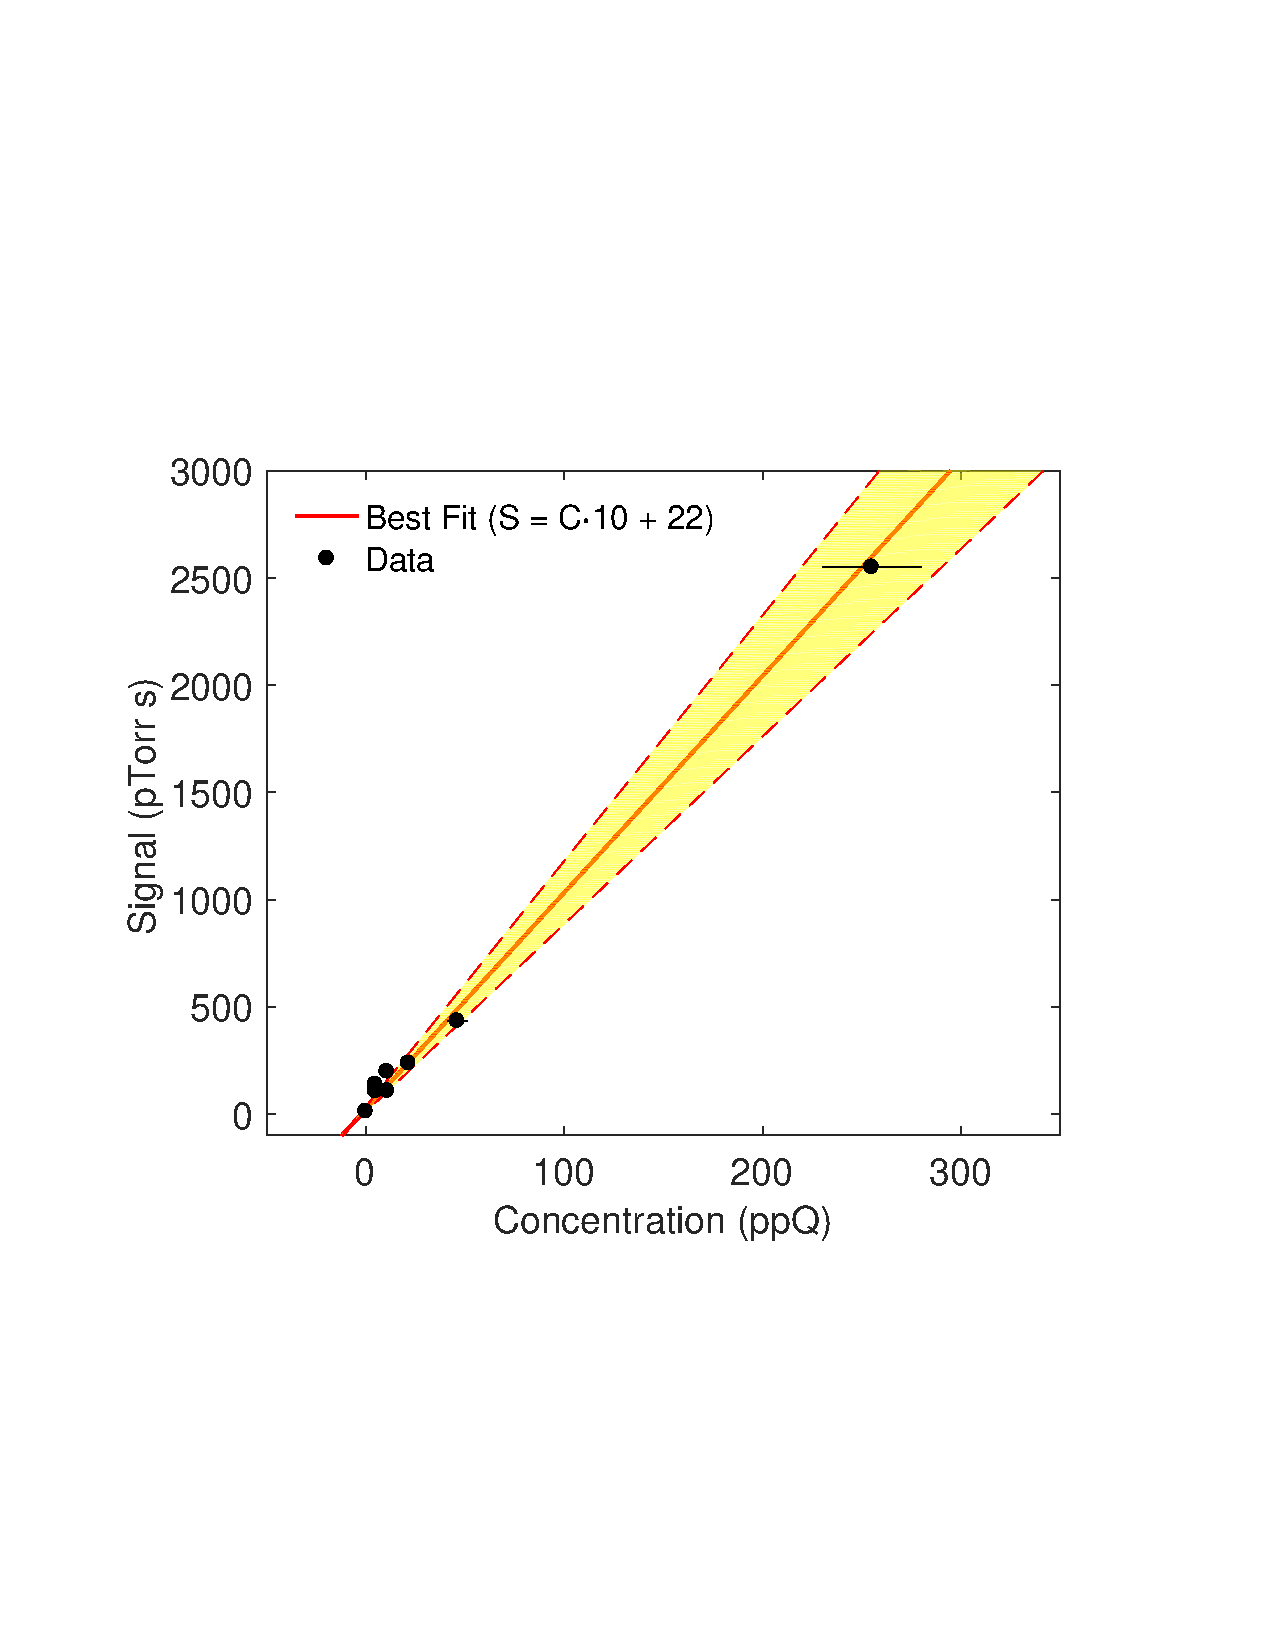
\includegraphics[width=\textwidth]{Figures/LinPlot0217.png}
  \caption{Linearity of analysis.}
  \label{fig:intlin}
\end{subfigure}
\caption{Linearity of the integration-style analysis described in equation \ref{eq:int_analysis}. The krypton signals used in these measurements never reached an equilibrium value. The xenon flow profile for theses measurements was a square pulse. The height of this pulse was set using an MFC, and the time-width of the pulse was defined by the size of the xenon sample used. $t_1$ was defined as the start of the xenon flow, plus 20 seconds, and $t_2$ was defined as the stop of the xenon flow, plus 20 seconds.}
\label{fig:linplot}
\end{figure}

The random uncertainty of purity results calculated using equation \ref{eq:int_analysis} are harder to estimate than those calculated using equation \ref{eq:average_analysis}. The fluctuations around each datapoint cannot be measured directly, so they are estimated using the baseline data collected in region I. The fluctuations of the RGA tend to increase at higher partial pressure, as shown in figure \ref{fig:RGAnoise}. We take the baseline fluctuations, $\sigma_0$, to be equal to the standard deviation of the region I data points. The random uncertainty of each data point, $PP_{Kr,i}$, is then taken to be:
{\color{red}
\begin{equation}
\label{eq:preserr}
\sigma_i=\sigma_{0}*(1+0.009*PP_{Kr,i}).
\end{equation}}
The propagation of this error to $\Phi$ is then:
\begin{equation}
\sigma_{\Phi}^2=\frac{1}{F_{Q,t_1,t_2}^2C^2}\sum_{i=1}^{N}(\sigma_i^2+\sigma_0^2/N_B)\Delta t_i^2,
\end{equation}
where $N_B$ is the number of data points used in the calculation of $\overline{PP}_{Kr,0}$ and $\sigma_0$.
\begin{figure}[h!]
  \includegraphics[width=\linewidth]{Figures/RGA_Noise_v_PP.png}
  \caption{The trend in RGA fluctuations as a function of partial pressure. The noise ratio is defined as the fraction by which the RGA fluctuations increase when the partial pressure is increased from its baseline value ($\textrm{Noise ratio} \equiv \sigma(PP)/\sigma(baseline)$). }
  \label{fig:RGAnoise}
\end{figure}


\section{System Parameters and Optimization}
Optimizing a cold-trap sampling system is a matter of maximizing the signal to noise ratio, which comes down to minimizing the fluctuations in the RGA baseline and maximizing the system response to krypton. There are several knobs and dials to turn to achieve this, but adjusting one of the knobs might change how one of the dials affects the sensitivity. This section will attempt to catalog the affect of these adjustments in an empirical way and will describe the optimal arrangement.
 

\subsection{RGA Parameters} 
The first and simplest adjustments to be made are to the RGA electronics. These adjustments can be made quickly and easily, and are largely independent from the other knobs and dials. There is a long list of internal RGA parameters which should be understood before operating a cold trap system. These can be found in chapter 6 of the \href{http://www.thinksrs.com/downloads/PDFs/Manuals/RGAm.pdf}{RGA manual}. The two parameters that have the greatest effect on the sensitivity to krypton are the noise floor and the high-voltage setting of the continuous dynode electron multiplier (CDEM). 

The noise floor sets the scan speed of the RGA; the lower the noise floor setting, the longer the RGA will spend integrating current on a single mass point. The practical effects are threefold. The obvious first implication is that with a low noise floor, it will take much longer to to collect a single data point. At a noise floor setting of 0 the RGA will sit on a mass point for more than 5 seconds, and at a noise floor setting of 3 it will sit for less than 0.5 seconds per mass. For high-sensitivity analysis, it is better to have the noise floor set as low as possible, which will give you fewer data points which have a smaller variance. This will reduce the amount of time spent communicating with the RGA, as well as the amount of down time between communications. 

{\color{red}At higher noise floors, there tends to be an offset in the baseline. While we usually try to account for this by using baseline-subtracted pressures in purity calculations, it is possible that the shifted baseline is not additive to the pressure signal. This is indicated by the krypton signal in the LUX run04 data decreasing artificially. There is also evidence from the SLAC system that the baseline is not strictly additive to a physical pressure signal.}

Setting the voltage on the CDEM is a balancing act. Increasing the voltage increased the signal amplification. Above a certain CDEM voltage, however, the random fluctuations in the RGA baseline rise faster than the gain, and if the voltage is set too high, the xenon ice vapor pressure will begin saturate the CDEM, degrading and possibly damaging it. The CDEM voltage should be high enough that the largest xenon peaks such as 132 and 133 should be at saturation but not so high that the doubly ionized peaks such as 66 amu saturate. 
\begin{figure}[h]
  \includegraphics[width=\linewidth]{Figures/CDEM_gain_noise.png}
  \caption{RGA sensitivity as a function of CDEM voltage. }
  \label{fig:CTpid}
\end{figure}

The health of the CDEM can be tracked using one of the xenon ice peaks, assuming the MG and SP parameters are not changed. MG is the CDEM gain factor and SP is the mass sensitivity factor used to convert the RGA current to partial pressure. The physical values may change over time, but the parameter stored in the RGA memory will not change unless a head-calibration is run. In particular, as the CDEM degrades, the gain will fall. A drift in the gain will bee seen most easily as a drop in the measured xenon ice pressure. Since the vapor pressure of xenon ice at 77 Kelvin is physically constant, if this pressure reading drops, it indicates that the gain has dropped. To maintain the CDEM gain, the xenon peak at 62 amu should be monitored. Whenever this value drops, the voltage should be increased until the pressure returns to its initial value.


\subsection{Impedance and Flow Rate Settings}
Consider the idealized pressure trace shown in figure \ref{fig:RGAtrace_ideal}, which is the result of a rectangular flow rate profile into a system which has an instantaneous response. The flat top of this trace will have a height given by equation \ref{eq:krpres2}:
\begin{equation}
PP_{Kr,eq}=\frac{\alpha}{180}Z_{1}Q_{Xe,CT}\Phi_{Kr}.
\end{equation}
The width of this pulse will be given by the amount of xenon used in the analysis ($V_{SB}\Delta P_{Xe,SB}$) divided by the flow rate of the xenon into the cold trap $Q_{Xe,CT}$.  Assume $N$ is the number of data points included in the analysis. Using a constant RGA sampling rate of $r$ we find: 
\begin{equation}
N=\frac{rV_{SB}\Delta P_{Xe,SB}}{Q_{Xe,CT}}.
\end{equation}
By increasing the flow, we get something of a tradeoff. The pressure which we are trying to measure will increase proportionally to $Q_{Xe,CT}$. However the number of data-points in our analysis will also decrease proportionally to $Q_{Xe,CT}$, thereby increasing the uncertainty. Since uncertainty only has a dependence on $\sqrt{N}$, we will end up winning in signal-to-noise ratio, which will increase proportional to $\sqrt{Q_{Xe,CT}}$. 
\begin{figure}[h]
  \includegraphics[width=\linewidth]{Figures/RGAtrace_ideal.png}
  \caption{Peak krypton RGA pressure as a function of flow rate.  }
  \label{fig:flowresponse1x}
\end{figure}

The dependence of our idealized signal-to-noise on $\sqrt{Q_{Xe,CT}}$ argues for the use of as high a xenon flow rate as possible. Unfortunately, we don't live in an ideal world, and there are forces conspiring against us in the high-flow limit. In section \ref{sec:flow_real} we saw that at flow rates above about 2 SLM, the krypton throughput begins to fall. This effect will compete with, and may even overwhelm the statistical benefit we get from increasing the flow rate.

We are in a similar situation with our impedance setting. We have shown in section \ref{sec:impedance_real} that it is possible to amplify $PP_{Kr}$ by modifying the impedances of IV1 and IV2. Figure \ref{fig:ampimp} show a krypton signal which is nearly buried in electronic RGA noise can be increased more than ten-fold by adjusting the impedances. This amplification is not perfect, and comes at the cost of longer rise times and decreased krypton throughput. Even with these competing effects, the krypton equilibrium pressure remains monotonically increasing in $Z_1$ as far as we have been able to measure.
\begin{figure}[h]
  \includegraphics[width=\linewidth]{Figures/Adjusted_impedance_study.png}
  \caption{Amplification of krypton signal by increasing the impedance settings to the 50x state. Identical flow rates and xenon samples were used with the only difference being the impedance settings. $\Phi$ is the measured krypton concentration in the 1x impedance setting and corresponding calibration. $\Phi_{eff}$ is the equivalent measurement in the 50x state, using the 1x calibration number.  }
  \label{fig:ampimp}
\end{figure}

To this point we have not yet developed a fully armed and operational model as to the physical chemistry governing the freezing of the xenon and the flow of xenon. The toy models we have developed provide some useful insights as to how to optimize the system, but significant tension with the data. In order to find the optimal settings for out cold trap system we turn instead to brute-force, empirical methods. We conduct a series of analysis-style runs at varying impedances and flow rates.  The analysis procedure is standardized such that the only variables remaining are impedance and flow rate. The krypton concentration, RGA setting, and even ice-kernel formation procedure is identical for all the tests in the series. We choose an impedance setting and then scan through a series of flow rates. Once we are satisfied that we have located the optimal flow rate for that impedance, we move on to the next  impedance setting.
\begin{figure}[h]
  \includegraphics[width=\linewidth]{Figures/SLAC_flowimpedance_response_plot.png}
  \caption{Scan across impedance and flow rate setting in search of the optimal settings.}
  \label{fig:sensscan}
\end{figure}

For each setting, we conduct an integration-style analysis on the $PP_{Kr}(t)$ data to get an integrated pressure signal:
\begin{equation}
 X_{Z,Q}=\sum_{i=1}^{N}(PP_{Kr,i}-\overline{PP_{Kr,0}})\Delta t_i,
 \end{equation}
along with its corresponding uncertainty, $\sigma_{Z,Q}$. We use the $X_{Z,Q}$'s and $\sigma_{Z,Q}$'s to extrapolate a sensitivity, ($\phi_{sens}(Z,Q)$) for each setting:
\begin{equation}
\phi_{sens}(Z,Q)=\Phi_{sample}\frac{\sigma_{Z,Q}}{X_{Z,Q}},
\end{equation}
where $\Phi_{sample}$ is the known concentration of the xenon sample. 

The minimum extrapolated sensitivity we measured during this scan was 4.5 ppQ, at 130x impedance and a flow rate of 2.4 SLM. Past about 30x impedance, the we find only a small benefit in increasing the impedance. The benefit of going from 37x impedance to 130x impedance is only about a 6\% drop in extrapolated sensitivity, whereas the benefit to going from 11x to 37x is a 22\% drop. Additionally, the optimal settings are all in the high xenon flow regime, but the high-impedance optimizations are near the transition point. The optimal flow for the 130x impedance is only 2.5 SLM, putting it essentially on the transition point between high and low flow regimes.

For the purposes of our final system optimization, we want to set the impedance as high as possible but will not go to the full 130x for reasons of practicality. With higher set points, the impedance becomes increasingly difficult to set repeatably. This, combined with the marginal impedance dependance above the 30x  set-point leads us to aim for an impedance set-point of 90x. The optimal flow rate at this impedance is between 2.5 and 3 SLM, so we use 2.5 SLM as our MFC set-point.



\section{Preparation of Calibration Xenon}
\label{sec:calprep}
Once the system has been optimized using a largely arbitrary mixture of xenon and krypton, the next key step is to measure the response of the system to a series of mixtures referred to as calibration xenon which have well known concentrations of krypton. Once this response is known, the system can be used to measure concentrations of unknown mixtures. To this end, the preparation of a mixture of xenon and krypton with a well known concentration is essential.

The first ingredient in the preparation of this mixture is extremely pure xenon. This is obtained by using the cold trap system itself to clean a small amount of stock xenon. As was explained previously, the cold trap analysis works because all but a microscopic amount of xenon is retained by the cold trap, while gasses such as krypton pass through largely unaffected. This means that the xenon that remains in the cold trap after an analysis has significantly lower krypton content than before the analysis. Depending on the system parameters, the post-run xenon will contain as little as $1/15^{\textrm{th}}$ the krypton as the pre-run xenon. Using the system described by figure \ref{fig:SLACpid}, it takes about 3 hours to purify 100g of typical stock xenon with a concentration of 1 part in $10^{9}$ down to $< 1$ part in $10^{15}$, 
\begin{figure}[h!]
  \includegraphics[width=\linewidth]{Figures/Mixing_diagram.png}
  \caption{Plumbing diagram of a generalized mixing system. }
  \label{fig:mixpid}
\end{figure}

Once the xenon has been cleaned it is transferred to an appropriate mixing system, described by figure \ref{fig:mixpid}. The relative volumes of this system must be extremely well known, so they are measured using volume sharing. First the full system, including injection, expansion, and xenon spaces, is filled with roughly 2000 torr of xenon as measured by pressure transducer 1. Then the expansion space is pumped to vacuum, leaving a well known pressure in both the injection and xenon spaces. Valve 4 is opened to expose the gas within the xenon space to the expansion space. The resulting pressure on PT1 gives the volume of the expansion space relative to the xenon space. Through the ideal gas law, when temperature is constant and mass is conserved, pressure times volume will remain constant:
\begin{equation}
P_{1}V_{Xe} = P_{2}(V_{Xe}+V_{inj})
\end{equation}
Therefore, the volume of the expansion space relative to the xenon space can be calculated using:
\begin{equation}
\frac{V_{inj}}{V_{Xe}} = \frac{P_{1}-P_{2}}{P_{2}}.
\end{equation}
The relative size of the injection space is then found in the same way. The absolute volumes can be measure by expanding from the expansion space into a space with an already known volume. Typically we use Swagelok DOT-compliant sample cylinders as our xenon space. These are fabricated to have a specified volume, so we calculate the absolute volume of the expansion and injection spaces by referencing this specified volume.

To prepare the calibration xenon, the injection space is filled to some known pressure with pure krypton. The krypton is then opened to the expansion space in order to reduce the pressure, and then the expansion space is pumped out using a the turbo-pump until PT2 reads $<1\times10^{-6} \textrm{ torr}$. This expansion is repeated until the desired krypton pressure is reached. After the final expansion volume pump-out, the xenon space is opened to the injection volume, and the new xenon/krypton mixture is frozen back into the xenon volume using liquid nitrogen. The krypton concentration ($\Phi_{Kr}$) of the calibration xenon in grams krypton per grams xenon is given by:
\begin{equation}
\Phi_{Kr} = \frac{a^{N}P_{Kr,0}V_{inj}\rho_{Kr} }{P_{Xe}V_{Xe}\rho_{Xe}},
\end{equation}
where the expansion ratio, $a$, is given by $V_{inj}/(V_{inj}+V_{expansion})$, $N$ is the number of expansions, $P_{Kr,0}$ and $P_{Xe}$ are the krypton and xenon pressures initially injected into the system, and $\rho_{Kr}=3.4692$ g/liter and $\rho_{Xe}=5.4535$ g/liter are the krypton and xenon gas densities.\cite{nist} 

Except for the densities, which are assumed to be exact, the pressures and volumes usually have comparable fractional uncertainties, with the exception of $V_{inj}$, which will be slightly dominant. After a few expansions this dominance becomes more pronounced. If we keep in mind the definition of $a$ from above, we find the following expression for the uncertainty on $\Phi_{Kr}$:
\begin{equation}
\sigma_{\Phi}^{2} = \Phi_{Kr}^2\left[  \left((N+1)\frac{\sigma_{V_{inj}}}{V_{inj}}\right)^2 + \left(N\frac{\sigma_{V_{exp}}}{V_{exp}}\right)^2  + \left(\frac{\sigma_{P_{Kr}}}{P_{Kr}}\right)^2   + \left(\frac{\sigma_{P_{Xe}}}{P_{Xe}}\right)^2   + \left(\frac{\sigma_{V_{Xe}}}{V_{Xe}}\right)^2  \right].
\end{equation}
This expression is not a perfect estimation of the error on the uncertainty. Typically either $V_{inj}$ will be used to measure $V_{exp}$, or vice versa. To incorporate the effects of correlated uncertainties, we can run the calculations for volume measurements and concentrations many times, randomly varying the pressure measurements and reference volume according to their respective uncertainties.

The final injection pressure must be kept above 0.01 torr to ensure the krypton remains above the molecular flow regime. This sets a lower limit on the concentration of calibration xenon that can be produced through this method. With an injection volume of 5cc and a xenon volume of 4000cc, the lowest concentration than can be produced from pure krypton is about 5 ppB. In order to produce calibration xenon with smaller concentrations, the pure krypton is replaced with the ppB level calibration xenon, which is diluted into clean xenon through the same process outlined in the previous paragraph.



\section{Sensitivity Demonstration at SLAC}
With our system optimized to the best of our ability, we predict that we will be able to measure krypton contamination in a xenon sample of roughly 5 ppQ gram per gram. Our procedure will utilize the results from all of our optimization studies. The RGA CDEM voltage was set such that the highest xenon peaks were saturating the data collection, and the doubly ionized $^{124}$Xe peak was reading 2300 pTorr. For our setup, this was 1750 Volts. The xenon flow rate used was 2.5 SLM, and the impedance was set to 90x. We used the modified technique of forming the ice kernel, using only ~50 standard cc and forming the kernel prior to fully submerging the trap in the LN bath. This technique was described in section \ref{sec:iceform}. 

For all of the tests in this demonstration we used a single sample of xenon. To initially prepare this sample, we filled our 4073 $\pm 5$ cc sample volume (the green section in figure \ref{fig:CTpid}) with 2720 $\pm 14$ Torr of xenon. Using the method described in section \ref{sec:calprep}, we cleaned this xenon to the point where were were no longer able to detect krypton. Into this clean xenon we mixed very small amounts of xenon which was previously-prepared with 274 ppB ``cocktail xenon''. After every analysis run, we would refreeze this xenon into SB, and then do whatever combination of cleaning and mixing was necessary to prepare for the next desired test.

\subsection{Blank Runs}
We analyze the RGA data from the 84 amu peak ($PP_{Kr,i}$) according to equation \ref{eq:int_analysis}, leaving off the constant term:
\begin{equation}
\label{eq:SLACintan}
X=\sum_{flow \  start+20sec}^{flow \ stop}(PP_{Kr,i}-\overline{PP_{Kr,0}})\Delta t_i.
\end{equation}
The error propagation for this is:
\begin{equation}
\sigma_{X}^2=\sum_{flow \  start+20sec}^{flow \ stop}(\sigma_i^2+\sigma_0^2/N_B)\Delta t_i^2,
\end{equation}
where $\sigma_i$ is defined by equation \ref{eq:preserr}. As before, $\overline{PP_{Kr,0}}$ is the average of the RGA readings at 84 amu prior to starting flow, $\sigma_0$ is the standard deviation of these points, and $N_B$ is the number of these points used. We will only include the data in the closed time interval starting 20 seconds after flow was started and ending at the time the flow stopped. This $X$ will be the figure of merit we use in establishing our limit of sensitivity. We will measure $X$ for a series of prepared concentrations of xenon, $\Phi$. If our system is working as predicted, the data ($\Phi,X$) will fit to a line with a slope equal to $F_{Q,t_1,t_2}C$.

Before demonstrating that the system is capable of a positive measurement, we first show that it is capable of measuring 0 ppQ. To do this we start with our newly cleaned xenon, and run a series of ``blank'' measurements in which we do not mix krypton into the xenon. The values of $X$ in these blank runs should fluctuate around 0 $pTorr\cdot s$, although there may be some offset due to RGA baseline issues. Our measurements bear this out. We ran 15 blank runs. The average value of $X$ for these runs was 10 pTorr seconds, and the standard deviation was 31 pTorr seconds. The average uncertainty on these points is $\sigma_X=26.2\pm0.8$ pTorr seconds.

There was one significant outlier in our blank data which had a value of 118 $\pm35$ pTorr seconds. We decided not to use this datapoint because the RGA baseline was acting up and had a clear periodicity. We made sure that our other measurements were take on top of an unvarying baseline.
\begin{figure}[h!]
  \includegraphics[width=\linewidth]{Figures/BlankHist0217.png}
  \caption{Histogram of measurements of xenon which has $<1$ ppQ of  krypton.}
  \label{fig:senstrace}
\end{figure}


\subsection{Mixing of ppQ Level Samples}
The previously mention 274 ppB cocktail xenon' was prepared using a separate system at the University of Maryland. The volumes of this system were measured by volume sharing as described in section \ref{sec:calprep}. The pressure gauge used was an MKS Baratron 722b capacitance manometer The accuracy of the 722b pressure gauge is 0.5\% of the reading. We also observe a constant zero offset of the gauge to be $0.8\pm0.5$ Torr which will be subtracted from the pressure readings. The absolute reference volume was a 500cc Swagelok DOT-compliant sample cylinder. The output of this bottle was modified to accommodate a 1/4 inch VCR B-series bellows valve. We take the volume of this space to be $500 \pm10$cc. This reference volume doubled as the xenon space. 

The volume of the injection space was measured to be $16.00 \pm 0.25$cc. The expansion ratio is $a=0.0261 \pm0.0008$. The starting xenon pressure was $841\pm4$ Torr in the 500cc xenon space. We injected an initial krypton pressure of $638\pm3$ Torr in the injection space. We expanded three times before mixing it with the xenon yielding a mixture with $276\pm25$ ppB (g Kr)/(g Xe).
\begin{figure}[h!]
  \includegraphics[width=\linewidth]{Figures/SLAC_ColdTrap_diagram_wvols.pdf}
  \caption{P\&ID of the SLAC sampling system.}
  \label{fig:SLACpid}
\end{figure}

The second-order mixings to dilute the 276 ppB cocktail xenon were done in-situ in the SLAC system. The SLAC sampling system is diagramed in figure \ref{fig:SLACpid}. The blue boxes and corresponding arrows indicate the various isolated spaces in the system, the volumes for which are listed in table \ref{tab:SLACvols}. The spaces of interest for mixing are spaces 1, 3, 4, 5, 6, and 7. The cocktail xenon is stored in space 6, the clean xenon is held in spaces 1, and the injection volume is space 5. As our primary expansion volume we used space 4 and used spaces 7 and 3 to increase the volume as needed.
\begin{table}[h!]
\centering
 \label{tab:SLACvols}
 \begin{tabular}{ c | c | c }
 \hline
 \hline
 Space \# & Volume (cc) & $\pm$ (cc) \\ 
 \hline\hline
1 & 3864 & 10 \\ 
2 & 3837 & 10 \\
3 & 23.9 & 1.4 \\
4 & 186.3 &1.9 \\
5 & 4.92 & 0.09 \\
6 & 1000 & 5 \\
7 & 93.8 & 1.6 \\
8 & 221.0 & 4.9 \\
 \hline
 \hline
\end{tabular}
\caption{List of SLAC system volumes. Refer to figure \ref{fig:SLACpid} for descriptions of spaces.}
\end{table}

The cocktail xenon was initially at a pressure of $128.0\pm0.6$ Torr. Since we do not have a pressure gauge on space 6, every time we volume share with the injection volume, we calculate the new pressure contained in space 6. This calculation is simply the old pressure multiplied by the volume ratio (4.9 cc)/(4.9 cc+1000 cc)=0.0049.
 \begin{table}[h!]
 \centering
 \label{tab:concentrations}
 \begin{tabular}{ c | c | c | c | c | c}
 \hline
 \hline
 $\Phi$ (ppQ) & $\pm$ (ppQ) &  Expansion Spaces & $N_{exp}$ & $N_{inj}$ & $P_{inj}$ (Torr) \\ 
 \hline
 \hline
4.92 & 0.49 & 5+7 & 2 & 1 & 128 \\ 
4.90 & 0.49 & 5+7 & 2 & 1 & 127.4 \\ 
10.8 & 1.1 & 5 & 2 & 1 &126.8 \\
21.6 & 2.2 & 5 & 2 & 2 & 126.3,125.8 \\
46.1 & 4.9 & (5),(5+3) & 1,1 & 1* & 125.2 \\
10.7 & 1.1 & 5 & 2 & 1 & 124.6 \\
255 & 24 & 5+7+3 & 1 & 1 & 124.0 \\
 \hline
 \hline
\end{tabular}
\caption{Parameters of the sample concentrations used to demonstrate the sensitivity of the SLAC system. The indicated uncertainties do not include the 7\% systematic uncertainty from the cocktail xenon concentration.}
\end{table}

The procedure for mixing follows the same outline as in section \ref{sec:calprep}. We select a desired sample concentration ($\Phi_{Kr}$), choose the appropriate expansion space ($V_{exp}$), expand the required number of times ($N_{exp}$), and then mix the remaining cocktail xenon into the clean sample xenon. The resulting concentration will be given by:
\begin{equation}
\Phi_{Kr}=\frac{(274 \ ppB)\cdot (4.9 \ cc)\cdot P_{inj}}{(4073 \ cc)\cdot (2720 \ Torr)}\left(\frac{4.9 \ cc}{4.9 \ cc + V_{exp}}\right)^{N_{exp}}
\end{equation}
The actual values used in the preparation of our ppQ level samples are listed in table \ref{tab:concentrations}. The total expansion volume will be equal to the sum of volumes indicated in the ``Expansion Spaces'' column. There are two samples with slightly altered mixing procedures. The 21.6 ppQ sample was prepared by completing two consecutive injections using the same mixing parameters in order to approximately double the previous 10.3 ppQ concentration. The 46.1 ppQ sample was prepared in a slightly more complex way. We first filled the injection volume (space 5) and expanded once into space 4 as usual. However, after pumping out the expanded cocktail xenon in space 4, we expanded into both space 4 and space 3. We then pumped out spaces 4 and 5, and mixed our clean sample xenon with the cocktail xenon that had expanded into space 3. The calculation for this concentration is then:
\begin{equation}
\Phi_{Kr}=\frac{(274 \ ppB)\cdot ( 24.4 \ cc)\cdot (125.2 Torr)}{(4073 \ cc)\cdot (2720 \ Torr)}\frac{4.9 \ cc}{189.2 \ cc }\frac{4.9 \ cc}{213.6 \ cc }
\end{equation}


\subsection{Measurements of ppQ Level Samples}
With the measurability of 0 established, and low-concentration xenon samples in hand, we move to measure the sensitivity limit of the SLAC sampling system. To do this we first measure $X$ as described in equation \ref{eq:SLACintan} for each of the samples listed in table \ref{tab:concentrations}, and then fit a line to the set of ($\Phi_{Kr},X$). The data and best-fit line are shown in figure \ref{fig:linplot2017}. The slope of the best fit line is $10.1 \pm 1.4$ pTorr seconds/ ppQ, and the intercept is $22 \pm 12$ pTorr seconds. 
\begin{figure}[h!]
\centering
\begin{subfigure}{0.5\textwidth}
  \centering
  \includegraphics[width=\textwidth]{Figures/SensPlot0217.eps}
  \caption{Zoom in near limit of sensitivity.}
  %\label{}
\end{subfigure}%
\begin{subfigure}{0.5\textwidth}
  \centering
  \includegraphics[width=\textwidth]{Figures/LinPlot0217.eps}
  \caption{Overall linearity.}
  %\label{fig:intlin}
\end{subfigure}
\caption{}
\label{fig:linplot2017}
\end{figure}

The limit of sensitivity will be defined as the concentration at which 90\% of analyses will produce results greater than 1-$\sigma$ above a 0 ppQ measurement. Our 0 ppQ measurements have a signal of 10 $\pm$31 pTorr seconds. The lowest-concentration measurements ($<30$ ppQ) deviate off of the best fit line by 46 pTorr seconds, so the 90\% confidence limit at any concentration will be 59 pTorr below the best fit line. Putting this together, we are looking for the concentration at which the best fit line drops crosses 100 pTorr seconds. This puts our limit of sensitivity at 7.7 $\pm 2.0$ ppQ.


\begin{figure}[h!]
  \includegraphics[width=\linewidth]{Figures/SLAC_PvT_ppq_sensitivity.png}
  \caption{Krypton pressure vs time traces near the limit of sensitivity.}
  \label{fig:senstrace}
\end{figure}




























\chapter{LUX Post-Run 04 Calibration Campaign}
After the Run 04 WIMP-search was completed in June of 2016, the response of LUX detector was exercised using ER and NR calibration sources. 

\section{Mono-energetic Calibrations}
\subsection{Argon 37}
\subsection{Krypton 83}
\subsection{Xenon 131}

\section{Tritium and $^{14}$C Beta sources}
\subsection{Injection and Removal of CH$_{3}$T}
\subsection{Injection of $^{14}$CH$_4$}

\section{Efficiency Corrections from $^{37}$Ar, $^{131}$Xe$_{m}$, and $^{83}$Kr$_{m}$}
\subsection{S2 corrections from $^{37}$Ar}
\subsection{S1 corrections from $^{131}$Xe$_{m}$+$^{83}$Kr$_{m}$ Doke Plot}


\section{Model of Pathological S2 Tails derived from $^{131}$Xe$_{m}$ and Tritium}
\chapter{Detector Response to $^{14}$C Beta Decay}

\section{The Theoretical $^{14}$C Beta-Spectrum}
The shape of the theoretical spectrum of the carbon-14 beta decay has been of interest in the context neutrino mass experiments\cite{C14_Wietfeldt}, where the goal is to measure the precise endpoint, and in liquid scintillator experiments, which have $^{14}$C as a major background and so need to model the spectrum with high precision\cite{C14_Borexino, C14_Bergeron}. This  decay also is of interest in theoretical nuclear physics because it has an abnormally long half life\cite{C14_Kuzminov,C14_Genz,C14_Garcia}. This extended half life hints that there is some cancellation in the lowest order terms of the nuclear matrix element and higher order terms must be taken into consideration. This would also mean that there could be momentum-dependent deviations from the allowed spectral shape. There have been several experiments\cite{C14_Sonntag,C14_Wietfeldt,C14_Borexino,C14_Kuzminov,C14_Bergeron} which have shown deviations from the allowed shape. These results, however, are in some tension with each other, as well as with previous measurements which show a purely allowed spectral shape\cite{C14_Curran}.

\subsection{The Allowed Spectrum}
Carbon-14 decays to the ground state of nitrogen-14 by way of an allowed Gamow-Teller transition. This decay has a Q-value of 156 keV and a half life of 5730 years. In general, the theoretical spectrum for this decay takes the form\cite{C14_Kuzminov}:
\begin{equation}\label{eq:beta_spec}
\frac{dN}{dE}=\frac{1}{2\pi^3} \xi C(E) F(Z,E) p(E_0-E)^2
\end{equation}
Here, $p$ and $E$ are the momentum and total energy of the emitted beta, and $E_0$ is the endpoint energy of the spectrum. In equation \ref{eq:beta_spec} we have neglected the neutrino mass as well as a radiative correction term which is expected to have $<1\%$ effect on the shape of the spectrum\cite{C14_Wietfeldt}. The initial distribution of momentum between the electron and neutrino is proportional to $p(E_0-E)^2$. This is derived by the phase space density of free particles and will be referred to as the phase space factor. The Fermi function $F(Z,E)$ contains information about the interaction between the emitted beta and the daughter nucleus. The terms $\xi$ and  $C(E)$ represent the energy independent and energy independent parts of the nuclear matrix element.

\subsection{The Fermi Function}\label{sec:fermifunc}
As the emitted beta travels away from the daughter nucleus, the two interact and either increase or decrease the momentum of the beta, depending on its charge. In the case of $^{14}C$, the beta has a negative charge and has to climb up out of the electric potential created by the $^{14}N$ daughter nucleus. The resulting observed beta spectrum will then be pulled to lower energy than the initial phase space factor. This modification to the spectrum if known as the Fermi function, $F(Z,E)$. The traditional derivation of $F(Z,E)$ begins by assuming the daughter nucleus is a fixed point charge and then evaluates the electron wave-function given the resulting field. The wave function is only evaluated down to the nuclear radius, $R$, in order to avoid divergence\cite{wilkinson}:
\begin{equation}\label{eq:fermifunc1}
F(Z,E)=2(\gamma+1)\Gamma(2\gamma+1)^{-2}(2pR)^{2(\gamma-1)}e^{\pi \alpha Z E/p}|\Gamma(\gamma+i\alpha ZE/p)^{2}|^2
\end{equation}

There is also a much simpler closed-form solution in the low-Z, non-relativistic approximation\cite{beta_fermi}:
\begin{equation}\label{eq:fermifunc2}
F_{NR}(Z,E)=\frac{x}{1-exp(-x)},
\end{equation}
where $x=2\pi Ze^{2}/\hbar v$. Here, $Z$ is the atomic number of the daughter nucleus, $e$ is the electron charge, and $v$ is the final velocity of the beta particle. 

Electrons in the higher-momentum part of the spectrum will have velocities exceeding 0.5c, so the non-relativistic approximation may not hold. This being the case, we consider the Bethe-Bacher approximation, which estimates the relativistic correction\cite{beta_fermi,bethe}:
\begin{equation}\label{eq:fermifunc3}
F_{BB}(Z,E)=F_{NR}(Z,E)[W^2(1+4\gamma^2)-1]^S,
\end{equation}
where $W\equiv E/m_ec^2$, $\gamma \equiv \alpha Z$, and $S\equiv (1-\gamma^2)^{1/2}-1)$. The full relativistic Fermi function can be estimated by a series expansion on powers of $(\alpha Z)$\cite{wilkinson,C14_Wietfeldt}. This sum is of limited use to us here because it becomes invalid at low kinetic energy and in fact diverges at zero.

The final correction to the Fermi function we consider is the correction for screening of the Coulomb potential by the orbital electrons. This essentially amounts to a shift in the origin of $F(Z,E)$\cite{C14_Wietfeldt,beta_screening}:
\begin{equation}\label{eq:fermifunc4}
F_{S}(Z,E)=\frac{E'p'}{Ep}F(Z,E'),
\end{equation}
where $E'=E-V_0$ and $p'$ is is the associated momentum. For the $^{14}$C beta decay, $V_0=495$eV\cite{C14_Wietfeldt}.

Figure \ref{fig:C14_spec_corrs} compares the non-relativistic approximation to the various corrections described in this section. We can see that the Wilkinson expansion differs from $F_{NR}(7,E)$ by less than a percent down to a few eV, at which point it diverges. The Bethe-Bacher approximation is similarly very close to $F_{NR}(7,E)$, but it does not display the same pathological behavior at the origin. The correction for electron screening peaks at 1.5\% at a kinetic energy of $T=3.5$keV. Because of the pathology in the Wilkinson expansion, we will take our Fermi function to be the combination of equations \ref{eq:fermifunc3} and \ref{eq:fermifunc4}:
\begin{equation}\label{eq:fermifunc5}
F(Z,E)=\frac{E'p'}{Ep}F_{NR}(Z,E')[(E'/m_ec^2)^2(1+4\gamma^2)-1]^S,
\end{equation}
with $F_{NR}(Z,E)$ as defined in equation \ref{eq:fermifunc2} and $E'$ and $p'$ as defined for eqaution \ref{eq:fermifunc4}.

\begin{figure}[h!]
\centering
\includegraphics[width=\textwidth]{Figures/FermiFunc_compare.pdf}
\caption{Correction factors for the $^{14}$C beta Fermi function. We compare the non-relativistic approximation, $F_{NR}(7,E)$ to the relativistic corrections described in section \ref{sec:fermifunc}, as well as the non-relativistic function after having been adjusted to account for screening by the orbital electrons. Plotted is $|F'(7,E)-F_{NR}(7,E)|/F_{NR}(7,E)$, where $F'(7,E)$ are the adjusted Fermi functions as indicated in the legend.} 
\label{fig:C14_spec_corrs}
\end{figure}

\subsection{The Shape Factor}
For a typical allowed decay, the shape factor is dominated by interference between the Gammow-Teller axial matrix element, $\langle GT \rangle$ and the weak magnetism matrix element, $\langle WM \rangle$. Such a shape factor has the form\cite{C14_Kuzminov,C14_Garcia,C14_Wietfeldt,beta_Calaprice}:
\begin{equation}\label{eq:shapefactor1}
C(E)\approx1+\frac{4}{3M}\frac{\langle WM \rangle}{\langle GT \rangle}[E-E_0/2-m_e^2/E],
\end{equation}
where $M$ is the nucleon mass, $m_e$ is the electron mass, and $E_0$ is the endpoint energy of the beta-spectrum. Usually the energy dependence of $C(E)$ is small enough that it can be neglected, but in the $^{14}$C beta decay the suppressed decay rate means that $\langle GT \rangle$ is small enough to make its consideration necessary. Under the conserved vector current hypothesis (CVC), the weak magnetism matrix element can be analogized to that of an M1 electromagnetic transition ($\langle WM \rangle$=$\langle M1 \rangle$) for the purpose of calculating the expected shape factor.

There have been several calculations of the predicted shape factor\cite{C14_Garcia,C14_Wietfeldt,C14_Genz}. These typically use a more general form of the $C(E)$ which takes into account terms which have been neglected from equation \ref{eq:shapefactor1}:
\begin{equation}\label{eq:shapefactor2}
C(E)=1+aE+\mu_1\gamma_1b/E+cE^2,
\end{equation}
where $\gamma_1=[1+(\alpha Z)^2]^{1/2}$ and $\mu_1$ is a special Coulomb function. The coefficients $a$, $b$, and $c$ can be calculated using the appropriate matrix elements. The matrix elements are typically calculated using model wave functions for the $^{14}$C and $^{14}$N ground states.

The first measurement of the $^{14}$C shape factor was made by Sonntag et. al. in 1970\cite{C14_Sonntag}. In units of MeV, his measured shape factor was, $C(E)=1-9.14E+1.53/E+7.66E^2$. Genz et. al.\cite{C14_Genz} used this result in part to derive phenomenological wave functions which replicate the shape factor. Later experiments and theoretical calculations have rejected this shape factor.

Wietfeldt et. al. found their data to be consistent with a shape factor of $C(E)=1+aE$, with $a=-0.45 \text{ \ MeV}^{-1}$\cite{C14_Wietfeldt}. This result is very close to their own theoretical calculation of $a=-0.38 \pm 0.04 \text{ \ MeV}^{-1}$, along with theoretical calculations by Garcia and Brown\cite{C14_Garcia}, and  Calaprice and Holstein\cite{beta_Calaprice}. However, the best-fit value of $a$ was inconsistent depending on what range of energies was fit, and a second measurement of the spectrum 2 years later yielded a best fit parameter of $a=-0.63 \pm 0.05 \text{ \ MeV}^{-1}$. 

The Borexino collaboration attempted to measure the shape of the $^{14}$C beta spectrum using their counting test facility (CTF). They assumed the same functional form as the Wietfeldt paper and excluded all $a<-0.72 \text{ \ MeV}^{-1}$ with 90\% confidence\cite{C14_Borexino}. 


Most recently, V. Kuzminov and N. Osetrova measured the shape factor of then $^{14}$C beta decay using a wall-less proportional counter\cite{C14_Kuzminov}. They assumed a shape factor with the form, $C(E)=1+\beta(Q-T)$, with $Q$ being the endpoint energy and $T$ being the kinetic energy of the electron. They measured $\beta=1.24 \pm0.04 \text{ \ MeV}^{-1}$, which is in agreement with a theoretical calculation by . This result is equivalent to $a=0.68 \pm0.02 \text{ \ MeV}^{-1}$ in a Wietfeldt-style shape factor.



\section{Measurement of the Shape of the $^{14}$C Beta-Spectrum}


\section{Measurement of Light and Charge Yields}


\section{Measurement of Recombination Fluctuations from $^{14}$C}

\appendix
\chapter{Yields Results}\label{sec:results_tables}
\section{Carbon-14 $\langle E_{true} \rangle$}


\begin{table}
    \centering % Center table    
    \resizebox{1.1\linewidth}{!}{%
\begin{tabular}{ | c || c | c || c | c || c | c || c | c || c | c || c | c || c | c || c | c || c | c || c | c || c | c || c | c || c | c || }
\hline
E-field (V/cm) &  \multicolumn{2}{c||}{43.2 $\pm$ 2.5} & \multicolumn{2}{c||}{52.6 $\pm$ 2.9} & \multicolumn{2}{c||}{64.8 $\pm$ 3.7} & \multicolumn{2}{c||}{79.8 $\pm$ 4.6} & \multicolumn{2}{c||}{97.8 $\pm$ 5.6} & \multicolumn{2}{c||}{119.6 $\pm$ 6.9} & \multicolumn{2}{c||}{146.7 $\pm$ 8.3} & \multicolumn{2}{c||}{180 $\pm$ 10} & \multicolumn{2}{c||}{219 $\pm$ 13} & \multicolumn{2}{c||}{268 $\pm$ 15} & \multicolumn{2}{c||}{329 $\pm$ 19} & \multicolumn{2}{c||}{405 $\pm$ 22} & \multicolumn{2}{c||}{484 $\pm$ 28}\\
\hline
energy bin \# & $\langle E_{true} \rangle$ & $\pm$ & $\langle E_{true} \rangle$ & $\pm$ & $\langle E_{true} \rangle$ & $\pm$ & $\langle E_{true} \rangle$ & $\pm$ & $\langle E_{true} \rangle$ & $\pm$ & $\langle E_{true} \rangle$ & $\pm$ & $\langle E_{true} \rangle$ & $\pm$ & $\langle E_{true} \rangle$ & $\pm$ & $\langle E_{true} \rangle$ & $\pm$ & $\langle E_{true} \rangle$ & $\pm$ & $\langle E_{true} \rangle$ & $\pm$ & $\langle E_{true} \rangle$ & $\pm$ & $\langle E_{true} \rangle$ & $\pm$\\
\hline
1 & 1.8 & 0.1 & 1.8 & 0.1 & 1.8 & 0.1 & 1.8 & 0.1 & 1.8 & 0.1 & 1.8 & 0.1 & 1.8 & 0.1 & 1.8 & 0.1 & 1.8 & 0.2 & 1.8 & 0.1 & 1.8 & 0.2 & 1.8 & 0.1 & 1.8 & 0.1 \\
\hline
2 & 2.3 & 0.1 & 2.3 & 0.1 & 2.3 & 0.1 & 2.3 & 0.1 & 2.3 & 0.1 & 2.3 & 0.1 & 2.3 & 0.1 & 2.3 & 0.1 & 2.3 & 0.2 & 2.3 & 0.1 & 2.3 & 0.2 & 2.3 & 0.1 & 2.3 & 0.1 \\
\hline
3 & 2.8 & 0.1 & 2.8 & 0.1 & 2.8 & 0.1 & 2.8 & 0.1 & 2.8 & 0.1 & 2.8 & 0.1 & 2.8 & 0.1 & 2.8 & 0.1 & 2.8 & 0.2 & 2.8 & 0.1 & 2.8 & 0.2 & 2.8 & 0.1 & 2.8 & 0.1 \\
\hline
4 & 3.3 & 0.1 & 3.3 & 0.1 & 3.3 & 0.1 & 3.3 & 0.1 & 3.3 & 0.1 & 3.3 & 0.1 & 3.3 & 0.1 & 3.3 & 0.1 & 3.3 & 0.1 & 3.3 & 0.1 & 3.3 & 0.2 & 3.3 & 0.1 & 3.3 & 0.1 \\
\hline
5 & 3.8 & 0.1 & 3.8 & 0.1 & 3.8 & 0.1 & 3.8 & 0.1 & 3.8 & 0.1 & 3.8 & 0.1 & 3.8 & 0.1 & 3.8 & 0.1 & 3.8 & 0.1 & 3.8 & 0.1 & 3.8 & 0.2 & 3.8 & 0.1 & 3.8 & 0.1 \\
\hline
6 & 4.3 & 0.1 & 4.3 & 0.1 & 4.3 & 0.1 & 4.3 & 0.1 & 4.3 & 0.1 & 4.3 & 0.1 & 4.3 & 0.1 & 4.3 & 0.1 & 4.3 & 0.1 & 4.3 & 0.1 & 4.3 & 0.1 & 4.3 & 0.1 & 4.3 & 0.1 \\
\hline
7 & 4.7 & 0.1 & 4.8 & 0.1 & 4.8 & 0.1 & 4.8 & 0.1 & 4.8 & 0.1 & 4.8 & 0.1 & 4.8 & 0.1 & 4.8 & 0.1 & 4.8 & 0.1 & 4.8 & 0.1 & 4.8 & 0.1 & 4.8 & 0.1 & 4.8 & 0.1 \\
\hline
8 & 5.5 & 0.3 & 5.5 & 0.3 & 5.5 & 0.3 & 5.5 & 0.3 & 5.5 & 0.3 & 5.5 & 0.3 & 5.5 & 0.3 & 5.5 & 0.3 & 5.5 & 0.3 & 5.5 & 0.3 & 5.5 & 0.3 & 5.5 & 0.3 & 5.5 & 0.3 \\
\hline
9 & 6.5 & 0.3 & 6.5 & 0.3 & 6.5 & 0.3 & 6.5 & 0.3 & 6.5 & 0.3 & 6.5 & 0.3 & 6.5 & 0.3 & 6.5 & 0.3 & 6.5 & 0.3 & 6.5 & 0.3 & 6.5 & 0.3 & 6.5 & 0.3 & 6.5 & 0.3 \\
\hline
10 & 7.5 & 0.3 & 7.5 & 0.3 & 7.5 & 0.3 & 7.5 & 0.3 & 7.5 & 0.3 & 7.5 & 0.3 & 7.5 & 0.3 & 7.5 & 0.3 & 7.5 & 0.3 & 7.5 & 0.3 & 7.5 & 0.3 & 7.5 & 0.3 & 7.5 & 0.3 \\
\hline
11 & 8.5 & 0.3 & 8.5 & 0.3 & 8.5 & 0.3 & 8.5 & 0.3 & 8.5 & 0.3 & 8.5 & 0.3 & 8.5 & 0.3 & 8.5 & 0.3 & 8.5 & 0.3 & 8.5 & 0.3 & 8.5 & 0.3 & 8.5 & 0.3 & 8.5 & 0.3 \\
\hline
12 & 9.5 & 0.3 & 9.4 & 0.3 & 9.4 & 0.3 & 9.5 & 0.3 & 9.4 & 0.3 & 9.5 & 0.3 & 9.5 & 0.3 & 9.4 & 0.3 & 9.4 & 0.3 & 9.4 & 0.3 & 9.4 & 0.3 & 9.4 & 0.3 & 9.4 & 0.3 \\
\hline
13 & 10.4 & 0.3 & 10.4 & 0.3 & 10.4 & 0.3 & 10.4 & 0.3 & 10.4 & 0.3 & 10.4 & 0.3 & 10.4 & 0.3 & 10.4 & 0.3 & 10.4 & 0.3 & 10.4 & 0.3 & 10.4 & 0.3 & 10.4 & 0.3 & 10.4 & 0.3 \\
\hline
14 & 11.4 & 0.3 & 11.4 & 0.3 & 11.4 & 0.3 & 11.4 & 0.3 & 11.4 & 0.3 & 11.4 & 0.3 & 11.4 & 0.3 & 11.4 & 0.3 & 11.4 & 0.3 & 11.4 & 0.3 & 11.4 & 0.3 & 11.4 & 0.3 & 11.4 & 0.3 \\
\hline
15 & 12.4 & 0.3 & 12.4 & 0.3 & 12.4 & 0.3 & 12.4 & 0.3 & 12.4 & 0.3 & 12.4 & 0.3 & 12.4 & 0.3 & 12.4 & 0.3 & 12.4 & 0.3 & 12.4 & 0.3 & 12.4 & 0.3 & 12.4 & 0.3 & 12.4 & 0.3 \\
\hline
16 & 13.4 & 0.3 & 13.4 & 0.3 & 13.4 & 0.3 & 13.4 & 0.3 & 13.4 & 0.3 & 13.4 & 0.3 & 13.4 & 0.3 & 13.4 & 0.3 & 13.4 & 0.3 & 13.4 & 0.3 & 13.4 & 0.3 & 13.4 & 0.3 & 13.4 & 0.3 \\
\hline
17 & 14.4 & 0.3 & 14.4 & 0.3 & 14.4 & 0.3 & 14.4 & 0.3 & 14.4 & 0.3 & 14.4 & 0.3 & 14.4 & 0.3 & 14.4 & 0.3 & 14.4 & 0.3 & 14.4 & 0.3 & 14.3 & 0.3 & 14.4 & 0.3 & 14.4 & 0.3 \\
\hline
18 & 15.4 & 0.3 & 15.4 & 0.3 & 15.4 & 0.3 & 15.4 & 0.3 & 15.4 & 0.3 & 15.4 & 0.3 & 15.4 & 0.3 & 15.4 & 0.3 & 15.4 & 0.3 & 15.3 & 0.3 & 15.3 & 0.3 & 15.3 & 0.3 & 15.3 & 0.3 \\
\hline
19 & 16.4 & 0.3 & 16.4 & 0.3 & 16.4 & 0.3 & 16.4 & 0.3 & 16.4 & 0.3 & 16.4 & 0.3 & 16.4 & 0.3 & 16.3 & 0.3 & 16.3 & 0.3 & 16.3 & 0.3 & 16.3 & 0.3 & 16.3 & 0.3 & 16.3 & 0.3 \\
\hline
20 & 17.4 & 0.3 & 17.4 & 0.3 & 17.4 & 0.3 & 17.3 & 0.3 & 17.3 & 0.3 & 17.3 & 0.3 & 17.3 & 0.3 & 17.3 & 0.3 & 17.3 & 0.3 & 17.3 & 0.3 & 17.3 & 0.4 & 17.3 & 0.4 & 17.3 & 0.4 \\
\hline
21 & 18.4 & 0.3 & 18.4 & 0.3 & 18.3 & 0.3 & 18.3 & 0.3 & 18.3 & 0.3 & 18.3 & 0.3 & 18.3 & 0.3 & 18.3 & 0.3 & 18.3 & 0.4 & 18.3 & 0.4 & 18.3 & 0.4 & 18.3 & 0.4 & 18.3 & 0.4 \\
\hline
22 & 19.4 & 0.3 & 19.3 & 0.3 & 19.3 & 0.3 & 19.3 & 0.3 & 19.3 & 0.3 & 19.3 & 0.3 & 19.3 & 0.4 & 19.3 & 0.4 & 19.3 & 0.4 & 19.3 & 0.4 & 19.3 & 0.4 & 19.3 & 0.4 & 19.3 & 0.4 \\
\hline
23 & 20.3 & 0.3 & 20.3 & 0.3 & 20.3 & 0.3 & 20.3 & 0.4 & 20.3 & 0.4 & 20.3 & 0.4 & 20.3 & 0.4 & 20.3 & 0.4 & 20.3 & 0.4 & 20.3 & 0.4 & 20.3 & 0.4 & 20.3 & 0.4 & 20.3 & 0.4 \\
\hline
24 & 21.3 & 0.3 & 21.3 & 0.3 & 21.3 & 0.3 & 21.3 & 0.4 & 21.3 & 0.4 & 21.3 & 0.4 & 21.3 & 0.4 & 21.3 & 0.4 & 21.3 & 0.4 & 21.3 & 0.4 & 21.3 & 0.4 & 21.2 & 0.4 & 21.2 & 0.4 \\
\hline
25 & 22.3 & 0.3 & 22.3 & 0.4 & 22.3 & 0.4 & 22.3 & 0.4 & 22.3 & 0.4 & 22.3 & 0.4 & 22.3 & 0.4 & 22.3 & 0.4 & 22.2 & 0.4 & 22.2 & 0.4 & 22.2 & 0.4 & 22.2 & 0.4 & 22.2 & 0.4 \\
\hline
26 & 23.3 & 0.4 & 23.3 & 0.4 & 23.3 & 0.4 & 23.3 & 0.4 & 23.3 & 0.4 & 23.3 & 0.4 & 23.2 & 0.4 & 23.3 & 0.4 & 23.2 & 0.4 & 23.2 & 0.4 & 23.2 & 0.4 & 23.2 & 0.4 & 23.2 & 0.4 \\
\hline
27 & 24.3 & 0.4 & 24.3 & 0.4 & 24.3 & 0.4 & 24.3 & 0.4 & 24.3 & 0.4 & 24.2 & 0.4 & 24.2 & 0.4 & 24.2 & 0.4 & 24.2 & 0.4 & 24.2 & 0.4 & 24.2 & 0.4 & 24.2 & 0.4 & 24.2 & 0.4 \\
\hline
28 & 25.3 & 0.4 & 25.3 & 0.4 & 25.3 & 0.4 & 25.2 & 0.4 & 25.2 & 0.4 & 25.2 & 0.4 & 25.2 & 0.4 & 25.2 & 0.4 & 25.2 & 0.4 & 25.2 & 0.4 & 25.2 & 0.4 & 25.2 & 0.4 & 25.2 & 0.5 \\
\hline
29 & 26.3 & 0.4 & 26.3 & 0.4 & 26.3 & 0.4 & 26.2 & 0.4 & 26.2 & 0.4 & 26.2 & 0.4 & 26.2 & 0.4 & 26.2 & 0.4 & 26.2 & 0.4 & 26.2 & 0.4 & 26.2 & 0.4 & 26.1 & 0.5 & 26.1 & 0.5 \\
\hline
30 & 27.3 & 0.4 & 27.3 & 0.4 & 27.2 & 0.4 & 27.2 & 0.4 & 27.2 & 0.4 & 27.2 & 0.4 & 27.2 & 0.4 & 27.2 & 0.4 & 27.2 & 0.5 & 27.2 & 0.5 & 27.2 & 0.5 & 27.1 & 0.5 & 27.1 & 0.5 \\
\hline
31 & 28.3 & 0.4 & 28.2 & 0.4 & 28.2 & 0.4 & 28.2 & 0.4 & 28.2 & 0.4 & 28.2 & 0.4 & 28.2 & 0.4 & 28.2 & 0.4 & 28.1 & 0.5 & 28.1 & 0.5 & 28.1 & 0.5 & 28.1 & 0.5 & 28.1 & 0.5 \\
\hline
32 & 29.2 & 0.4 & 29.2 & 0.4 & 29.2 & 0.4 & 29.2 & 0.4 & 29.2 & 0.4 & 29.2 & 0.4 & 29.2 & 0.5 & 29.2 & 0.5 & 29.1 & 0.5 & 29.1 & 0.5 & 29.1 & 0.5 & 29.1 & 0.5 & 29.1 & 0.5 \\
\hline
33 & 30.2 & 0.4 & 30.2 & 0.4 & 30.2 & 0.4 & 30.2 & 0.4 & 30.2 & 0.4 & 30.2 & 0.5 & 30.1 & 0.5 & 30.1 & 0.5 & 30.1 & 0.5 & 30.1 & 0.5 & 30.1 & 0.5 & 30.1 & 0.5 & 30.1 & 0.5 \\
\hline
34 & 31.2 & 0.4 & 31.2 & 0.4 & 31.2 & 0.4 & 31.2 & 0.4 & 31.2 & 0.5 & 31.1 & 0.5 & 31.1 & 0.5 & 31.1 & 0.5 & 31.1 & 0.5 & 31.1 & 0.5 & 31.1 & 0.5 & 31.1 & 0.5 & 31.0 & 0.6 \\
\hline
35 & 32.2 & 0.4 & 32.2 & 0.4 & 32.2 & 0.4 & 32.2 & 0.5 & 32.1 & 0.5 & 32.1 & 0.5 & 32.1 & 0.5 & 32.1 & 0.5 & 32.1 & 0.5 & 32.1 & 0.5 & 32.0 & 0.5 & 32.0 & 0.6 & 32.0 & 0.6 \\
\hline
36 & 33.2 & 0.4 & 33.2 & 0.4 & 33.2 & 0.4 & 33.2 & 0.5 & 33.1 & 0.5 & 33.1 & 0.5 & 33.1 & 0.5 & 33.1 & 0.5 & 33.1 & 0.5 & 33.1 & 0.5 & 33.0 & 0.6 & 33.0 & 0.6 & 33.0 & 0.6 \\
\hline
37 & 34.2 & 0.4 & 34.2 & 0.5 & 34.2 & 0.5 & 34.1 & 0.5 & 34.1 & 0.5 & 34.1 & 0.5 & 34.1 & 0.5 & 34.1 & 0.5 & 34.1 & 0.5 & 34.0 & 0.6 & 34.0 & 0.6 & 34.0 & 0.6 & 34.0 & 0.6 \\
\hline
38 & 35.2 & 0.5 & 35.2 & 0.5 & 35.1 & 0.5 & 35.1 & 0.5 & 35.1 & 0.5 & 35.1 & 0.5 & 35.1 & 0.5 & 35.0 & 0.6 & 35.0 & 0.6 & 35.0 & 0.6 & 35.0 & 0.6 & 35.0 & 0.6 & 34.9 & 0.6 \\
\hline
39 & 36.1 & 0.5 & 36.1 & 0.5 & 36.1 & 0.5 & 36.1 & 0.5 & 36.1 & 0.5 & 36.1 & 0.5 & 36.1 & 0.5 & 36.0 & 0.6 & 36.0 & 0.6 & 36.0 & 0.6 & 36.0 & 0.6 & 35.9 & 0.6 & 35.9 & 0.7 \\
\hline
40 & 37.1 & 0.5 & 37.1 & 0.5 & 37.1 & 0.5 & 37.1 & 0.5 & 37.1 & 0.5 & 37.0 & 0.5 & 37.0 & 0.6 & 37.0 & 0.6 & 37.0 & 0.6 & 37.0 & 0.6 & 36.9 & 0.6 & 36.9 & 0.7 & 36.9 & 0.7 \\
\hline
41 & 38.1 & 0.5 & 38.1 & 0.5 & 38.1 & 0.5 & 38.1 & 0.5 & 38.1 & 0.5 & 38.0 & 0.6 & 38.0 & 0.6 & 38.0 & 0.6 & 38.0 & 0.6 & 38.0 & 0.6 & 37.9 & 0.7 & 37.9 & 0.7 & 37.9 & 0.7 \\
\hline
42 & 39.1 & 0.5 & 39.1 & 0.5 & 39.1 & 0.5 & 39.1 & 0.5 & 39.0 & 0.5 & 39.0 & 0.6 & 39.0 & 0.6 & 39.0 & 0.6 & 39.0 & 0.6 & 38.9 & 0.6 & 38.9 & 0.7 & 38.9 & 0.7 & 38.8 & 0.7 \\
\hline
43 & 40.1 & 0.5 & 40.1 & 0.5 & 40.1 & 0.5 & 40.1 & 0.5 & 40.0 & 0.6 & 40.0 & 0.6 & 40.0 & 0.6 & 39.9 & 0.6 & 39.9 & 0.6 & 39.9 & 0.7 & 39.9 & 0.7 & 39.9 & 0.7 & 39.8 & 0.7 \\
\hline
44 & 41.1 & 0.5 & 41.1 & 0.5 & 41.0 & 0.5 & 41.0 & 0.5 & 41.0 & 0.6 & 41.0 & 0.6 & 41.0 & 0.6 & 40.9 & 0.7 & 40.9 & 0.6 & 40.9 & 0.7 & 40.8 & 0.7 & 40.8 & 0.7 & 40.8 & 0.8 \\
\hline
45 & 42.1 & 0.5 & 42.1 & 0.5 & 42.0 & 0.6 & 42.0 & 0.6 & 42.0 & 0.6 & 42.0 & 0.6 & 42.0 & 0.6 & 41.9 & 0.7 & 41.9 & 0.7 & 41.9 & 0.7 & 41.8 & 0.7 & 41.8 & 0.8 & 41.8 & 0.8 \\
\hline
46 & 43.1 & 0.5 & 43.1 & 0.5 & 43.0 & 0.6 & 43.0 & 0.6 & 43.0 & 0.6 & 42.9 & 0.6 & 42.9 & 0.6 & 42.9 & 0.7 & 42.9 & 0.7 & 42.9 & 0.7 & 42.8 & 0.8 & 42.8 & 0.8 & 42.7 & 0.8 \\
\hline
47 & 44.0 & 0.5 & 44.0 & 0.5 & 44.0 & 0.6 & 44.0 & 0.6 & 44.0 & 0.6 & 43.9 & 0.6 & 43.9 & 0.7 & 43.9 & 0.7 & 43.9 & 0.7 & 43.8 & 0.7 & 43.8 & 0.8 & 43.8 & 0.8 & 43.7 & 0.8 \\
\hline
48 & 45.0 & 0.6 & 45.0 & 0.6 & 45.0 & 0.6 & 45.0 & 0.6 & 44.9 & 0.6 & 44.9 & 0.7 & 44.9 & 0.7 & 44.8 & 0.7 & 44.8 & 0.7 & 44.8 & 0.8 & 44.8 & 0.8 & 44.7 & 0.8 & 44.7 & 0.9 \\
\hline
49 & 46.0 & 0.6 & 46.0 & 0.6 & 46.0 & 0.6 & 46.0 & 0.6 & 45.9 & 0.6 & 45.9 & 0.7 & 45.9 & 0.7 & 45.8 & 0.7 & 45.8 & 0.7 & 45.8 & 0.8 & 45.7 & 0.8 & 45.7 & 0.9 & 45.7 & 0.9 \\
\hline
50 & 47.0 & 0.6 & 47.0 & 0.6 & 47.0 & 0.6 & 46.9 & 0.6 & 46.9 & 0.7 & 46.9 & 0.7 & 46.9 & 0.7 & 46.8 & 0.8 & 46.8 & 0.8 & 46.8 & 0.8 & 46.7 & 0.9 & 46.7 & 0.9 & 46.6 & 0.9 \\
\hline
51 & 48.0 & 0.6 & 48.0 & 0.6 & 48.0 & 0.6 & 47.9 & 0.6 & 47.9 & 0.7 & 47.9 & 0.7 & 47.8 & 0.7 & 47.8 & 0.8 & 47.8 & 0.8 & 47.7 & 0.8 & 47.7 & 0.9 & 47.6 & 0.9 & 47.6 & 0.9 \\
\hline
52 & 49.0 & 0.6 & 49.0 & 0.6 & 48.9 & 0.6 & 48.9 & 0.7 & 48.9 & 0.7 & 48.8 & 0.7 & 48.8 & 0.8 & 48.8 & 0.8 & 48.8 & 0.8 & 48.7 & 0.9 & 48.7 & 0.9 & 48.6 & 0.9 & 48.6 & 1.0 \\
\hline
53 & 50.5 & 0.8 & 50.5 & 0.8 & 50.4 & 0.8 & 50.4 & 0.9 & 50.3 & 0.9 & 50.3 & 0.9 & 50.3 & 0.9 & 50.2 & 1.0 & 50.2 & 1.0 & 50.2 & 1.0 & 50.1 & 1.1 & 50.1 & 1.1 & 50.0 & 1.1 \\
\hline
54 & 52.4 & 0.8 & 52.4 & 0.8 & 52.4 & 0.9 & 52.3 & 0.9 & 52.3 & 0.9 & 52.3 & 0.9 & 52.2 & 1.0 & 52.2 & 1.0 & 52.2 & 1.0 & 52.1 & 1.1 & 52.1 & 1.1 & 52.0 & 1.2 & 52.0 & 1.2 \\
\hline
55 & 54.4 & 0.8 & 54.4 & 0.8 & 54.4 & 0.9 & 54.3 & 0.9 & 54.3 & 1.0 & 54.2 & 1.0 & 54.2 & 1.0 & 54.1 & 1.1 & 54.1 & 1.1 & 54.1 & 1.1 & 54.0 & 1.2 & 53.9 & 1.2 & 53.9 & 1.2 \\
\hline
56 & 56.4 & 0.9 & 56.4 & 0.8 & 56.3 & 0.9 & 56.3 & 1.0 & 56.2 & 1.0 & 56.2 & 1.0 & 56.2 & 1.0 & 56.1 & 1.1 & 56.1 & 1.1 & 56.0 & 1.2 & 56.0 & 1.2 & 55.9 & 1.3 & 55.9 & 1.3 \\
\hline
57 & 58.4 & 0.9 & 58.4 & 0.9 & 58.3 & 0.9 & 58.2 & 1.0 & 58.2 & 1.0 & 58.2 & 1.0 & 58.1 & 1.1 & 58.1 & 1.1 & 58.0 & 1.2 & 57.9 & 1.2 & 57.9 & 1.2 & 57.8 & 1.3 & 57.8 & 1.4 \\
\hline
58 & 60.3 & 0.9 & 60.3 & 0.9 & 60.3 & 1.0 & 60.2 & 1.0 & 60.1 & 1.1 & 60.1 & 1.1 & 60.1 & 1.1 & 60.0 & 1.2 & 59.9 & 1.2 & 59.9 & 1.3 & 59.9 & 1.3 & 59.8 & 1.4 & 59.7 & 1.4 \\
\hline
59 & 62.3 & 0.9 & 62.3 & 0.9 & 62.2 & 1.0 & 62.1 & 1.1 & 62.1 & 1.1 & 62.1 & 1.1 & 62.0 & 1.2 & 62.0 & 1.2 & 61.9 & 1.3 & 61.8 & 1.3 & 61.8 & 1.3 & 61.7 & 1.4 & 61.7 & 1.5 \\
\hline
60 & 64.3 & 0.9 & 64.3 & 0.9 & 64.2 & 1.0 & 64.1 & 1.1 & 64.0 & 1.1 & 64.0 & 1.2 & 64.0 & 1.2 & 63.9 & 1.2 & 63.8 & 1.3 & 63.8 & 1.4 & 63.8 & 1.4 & 63.6 & 1.5 & 63.6 & 1.5 \\
\hline
61 & 66.2 & 1.0 & 66.2 & 1.0 & 66.2 & 1.0 & 66.1 & 1.1 & 66.0 & 1.2 & 66.0 & 1.2 & 65.9 & 1.3 & 65.9 & 1.3 & 65.8 & 1.4 & 65.7 & 1.4 & 65.7 & 1.5 & 65.6 & 1.6 & 65.5 & 1.6 \\
\hline
62 & 68.2 & 1.0 & 68.2 & 1.0 & 68.1 & 1.1 & 68.0 & 1.2 & 68.0 & 1.2 & 67.9 & 1.2 & 67.9 & 1.3 & 67.8 & 1.3 & 67.7 & 1.4 & 67.7 & 1.5 & 67.6 & 1.5 & 67.5 & 1.6 & 67.5 & 1.7 \\
\hline
63 & 70.2 & 1.0 & 70.1 & 1.1 & 70.1 & 1.1 & 70.0 & 1.2 & 69.9 & 1.2 & 69.9 & 1.3 & 69.8 & 1.3 & 69.8 & 1.4 & 69.7 & 1.5 & 69.6 & 1.5 & 69.5 & 1.6 & 69.4 & 1.7 & 69.4 & 1.7 \\
\hline
64 & 72.1 & 1.1 & 72.1 & 1.1 & 72.0 & 1.2 & 71.9 & 1.2 & 71.9 & 1.3 & 71.8 & 1.3 & 71.8 & 1.4 & 71.7 & 1.4 & 71.6 & 1.5 & 71.5 & 1.6 & 71.5 & 1.6 & 71.4 & 1.7 & 71.3 & 1.8 \\
\hline
65 & 74.1 & 1.1 & 74.0 & 1.1 & 74.0 & 1.2 & 73.9 & 1.3 & 73.8 & 1.3 & 73.8 & 1.4 & 73.7 & 1.4 & 73.7 & 1.5 & 73.5 & 1.6 & 73.5 & 1.7 & 73.4 & 1.7 & 73.3 & 1.8 & 73.2 & 1.9 \\
\hline
66 & 76.0 & 1.1 & 76.0 & 1.2 & 75.9 & 1.2 & 75.9 & 1.3 & 75.8 & 1.4 & 75.7 & 1.4 & 75.7 & 1.5 & 75.6 & 1.5 & 75.5 & 1.6 & 75.4 & 1.7 & 75.3 & 1.8 & 75.2 & 1.9 & 75.2 & 1.9 \\
\hline
67 & 78.0 & 1.2 & 77.9 & 1.3 & 77.9 & 1.3 & 77.8 & 1.3 & 77.7 & 1.4 & 77.7 & 1.5 & 77.6 & 1.5 & 77.5 & 1.6 & 77.4 & 1.7 & 77.3 & 1.8 & 77.2 & 1.9 & 77.2 & 1.9 & 77.1 & 2.0 \\
\hline
68 & 80.4 & 1.4 & 80.4 & 1.5 & 80.3 & 1.5 & 80.3 & 1.5 & 80.2 & 1.6 & 80.1 & 1.7 & 80.0 & 1.7 & 80.0 & 1.8 & 79.8 & 1.9 & 79.7 & 2.0 & 79.6 & 2.1 & 79.6 & 2.2 & 79.4 & 2.3 \\
\hline
69 & 83.4 & 1.5 & 83.3 & 1.6 & 83.2 & 1.6 & 83.2 & 1.6 & 83.1 & 1.7 & 83.0 & 1.8 & 82.9 & 1.8 & 82.9 & 1.9 & 82.8 & 2.0 & 82.6 & 2.1 & 82.5 & 2.3 & 82.4 & 2.3 & 82.3 & 2.4 \\
\hline
70 & 86.3 & 1.5 & 86.2 & 1.6 & 86.1 & 1.7 & 86.1 & 1.7 & 86.0 & 1.7 & 85.9 & 1.9 & 85.9 & 1.9 & 85.7 & 2.0 & 85.6 & 2.1 & 85.5 & 2.2 & 85.3 & 2.4 & 85.3 & 2.4 & 85.1 & 2.5 \\
\hline
71 & 89.2 & 1.6 & 89.1 & 1.7 & 89.1 & 1.7 & 89.0 & 1.7 & 88.9 & 1.8 & 88.8 & 1.9 & 88.7 & 2.0 & 88.6 & 2.1 & 88.5 & 2.2 & 88.4 & 2.3 & 88.2 & 2.5 & 88.2 & 2.5 & 88.0 & 2.7 \\
\hline
72 & 92.1 & 1.7 & 92.0 & 1.8 & 92.0 & 1.8 & 91.9 & 1.9 & 91.8 & 1.9 & 91.7 & 2.1 & 91.6 & 2.1 & 91.5 & 2.3 & 91.4 & 2.4 & 91.2 & 2.5 & 91.0 & 2.7 & 91.0 & 2.7 & 90.7 & 3.0 \\
\hline
73 & 96.0 & 2.1 & 95.9 & 2.2 & 95.9 & 2.2 & 95.8 & 2.4 & 95.7 & 2.4 & 95.6 & 2.5 & 95.4 & 2.6 & 95.3 & 2.8 & 95.2 & 2.8 & 95.0 & 3.0 & 94.8 & 3.2 & 94.8 & 3.2 & 94.4 & 3.5 \\
\hline
74 & 100.9 & 2.3 & 100.8 & 2.3 & 100.7 & 2.4 & 100.5 & 2.6 & 100.5 & 2.6 & 100.3 & 2.7 & 100.2 & 2.9 & 99.9 & 3.1 & 99.9 & 3.1 & 99.6 & 3.3 & 99.5 & 3.5 & 99.4 & 3.6 & 99.0 & 3.9 \\
\hline
75 & 105.7 & 2.4 & 105.6 & 2.4 & 105.5 & 2.5 & 105.2 & 2.8 & 105.1 & 2.9 & 105.0 & 3.0 & 104.8 & 3.2 & 104.5 & 3.4 & 104.5 & 3.5 & 104.2 & 3.7 & 104.1 & 3.8 & 103.9 & 4.0 & 103.6 & 4.3 \\
\hline
76 & 110.5 & 2.6 & 110.4 & 2.7 & 110.3 & 2.8 & 109.9 & 3.2 & 109.8 & 3.2 & 109.6 & 3.4 & 109.4 & 3.6 & 109.1 & 3.8 & 109.0 & 3.9 & 108.7 & 4.1 & 108.6 & 4.2 & 108.3 & 4.4 & 108.0 & 4.7 \\
\hline
77 & 115.2 & 2.9 & 115.1 & 2.9 & 114.9 & 3.1 & 114.4 & 3.6 & 114.3 & 3.6 & 114.1 & 3.8 & 113.8 & 4.0 & 113.5 & 4.3 & 113.3 & 4.4 & 113.0 & 4.7 & 113.0 & 4.7 & 112.6 & 5.0 & 112.5 & 5.1 \\
\hline
78 & 119.8 & 3.3 & 119.6 & 3.3 & 119.3 & 3.6 & 118.8 & 4.0 & 118.7 & 4.1 & 118.7 & 4.1 & 118.2 & 4.5 & 117.9 & 4.8 & 117.5 & 5.0 & 117.3 & 5.2 & 117.2 & 5.3 & 116.7 & 5.6 & 116.8 & 5.6 \\
\hline
79 & 124.2 & 3.7 & 124.0 & 3.9 & 123.6 & 4.2 & 123.1 & 4.6 & 123.0 & 4.7 & 123.3 & 4.3 & 122.3 & 5.2 & 122.1 & 5.4 & 121.5 & 5.7 & 121.3 & 5.9 & 121.1 & 6.0 & 120.6 & 6.4 & 120.8 & 6.2 \\
\hline
80 & 128.5 & 4.6 & 128.1 & 4.9 & 127.6 & 5.2 & 127.1 & 5.6 & 127.1 & 5.7 & 126.5 & 5.9 & 126.4 & 6.2 & 126.2 & 6.4 & 125.3 & 6.9 & 125.2 & 7.0 & 124.7 & 7.1 & 124.2 & 7.5 & 124.3 & 7.0 \\
\hline
81 & 134.7 & 5.2 & 133.8 & 5.5 & 133.0 & 5.8 & 133.0 & 6.2 & 132.9 & 6.2 & 131.8 & 6.4 & 132.0 & 6.7 & 132.1 & 6.9 & 130.5 & 7.3 & 130.6 & 7.5 & 129.5 & 7.5 & 129.2 & 7.9 & 128.2 & 7.5 \\
\hline\hline
\end{tabular}}
\caption{Results for $\langle E_{true} \rangle = \langle N_{\gamma} \rangle/\langle N_{e} \rangle$ using the carbon-14, ``gfdcm'' corrected data. The error column shows the combination of the uncertainty due to bin width and de-smearing. The first column shows the index of the reconstructed energy bin in which the measurement was made.}% Add 'table' caption
\end{table}


\begin{table}
    \centering % Center table
    \resizebox{1.1\linewidth}{!}{%
\begin{tabular}{ | c || c | c || c | c || c | c || c | c || c | c || c | c || c | c || c | c || c | c || c | c || c | c || c | c || c | c || }
\hline
E-field (V/cm) &  \multicolumn{2}{c||}{43.2 $\pm$ 2.5} & \multicolumn{2}{c||}{52.6 $\pm$ 2.9} & \multicolumn{2}{c||}{64.8 $\pm$ 3.7} & \multicolumn{2}{c||}{79.8 $\pm$ 4.6} & \multicolumn{2}{c||}{97.8 $\pm$ 5.6} & \multicolumn{2}{c||}{119.6 $\pm$ 6.9} & \multicolumn{2}{c||}{146.7 $\pm$ 8.3} & \multicolumn{2}{c||}{180 $\pm$ 10} & \multicolumn{2}{c||}{219 $\pm$ 13} & \multicolumn{2}{c||}{268 $\pm$ 15} & \multicolumn{2}{c||}{329 $\pm$ 19} & \multicolumn{2}{c||}{405 $\pm$ 22} & \multicolumn{2}{c||}{484 $\pm$ 28}\\
\hline
energy bin \# & $\langle E_{true} \rangle$ & $\pm$ & $\langle E_{true} \rangle$ & $\pm$ & $\langle E_{true} \rangle$ & $\pm$ & $\langle E_{true} \rangle$ & $\pm$ & $\langle E_{true} \rangle$ & $\pm$ & $\langle E_{true} \rangle$ & $\pm$ & $\langle E_{true} \rangle$ & $\pm$ & $\langle E_{true} \rangle$ & $\pm$ & $\langle E_{true} \rangle$ & $\pm$ & $\langle E_{true} \rangle$ & $\pm$ & $\langle E_{true} \rangle$ & $\pm$ & $\langle E_{true} \rangle$ & $\pm$ & $\langle E_{true} \rangle$ & $\pm$\\
\hline
1 & 1.8 & 0.1 & 1.8 & 0.1 & 1.8 & 0.1 & 1.8 & 0.1 & 1.8 & 0.2 & 1.8 & 0.2 & 1.8 & 0.2 & 1.8 & 0.2 & 1.8 & 0.2 & 1.8 & 0.2 & 1.8 & 0.2 & 1.8 & 0.2 & 1.8 & 0.2 \\
\hline
2 & 2.3 & 0.1 & 2.3 & 0.1 & 2.3 & 0.1 & 2.3 & 0.1 & 2.3 & 0.2 & 2.3 & 0.2 & 2.3 & 0.2 & 2.3 & 0.2 & 2.3 & 0.2 & 2.3 & 0.2 & 2.3 & 0.2 & 2.3 & 0.2 & 2.3 & 0.2 \\
\hline
3 & 2.8 & 0.1 & 2.8 & 0.1 & 2.8 & 0.1 & 2.8 & 0.1 & 2.8 & 0.2 & 2.8 & 0.2 & 2.8 & 0.2 & 2.8 & 0.2 & 2.8 & 0.2 & 2.8 & 0.2 & 2.8 & 0.2 & 2.8 & 0.2 & 2.8 & 0.2 \\
\hline
4 & 3.3 & 0.1 & 3.3 & 0.1 & 3.3 & 0.1 & 3.3 & 0.1 & 3.3 & 0.1 & 3.3 & 0.1 & 3.3 & 0.2 & 3.3 & 0.2 & 3.3 & 0.2 & 3.3 & 0.2 & 3.3 & 0.2 & 3.3 & 0.2 & 3.3 & 0.2 \\
\hline
5 & 3.8 & 0.1 & 3.8 & 0.1 & 3.8 & 0.1 & 3.8 & 0.1 & 3.8 & 0.1 & 3.8 & 0.1 & 3.8 & 0.1 & 3.8 & 0.1 & 3.8 & 0.2 & 3.8 & 0.2 & 3.8 & 0.2 & 3.8 & 0.2 & 3.8 & 0.2 \\
\hline
6 & 4.3 & 0.1 & 4.3 & 0.1 & 4.3 & 0.1 & 4.3 & 0.1 & 4.3 & 0.1 & 4.3 & 0.1 & 4.3 & 0.1 & 4.3 & 0.1 & 4.3 & 0.1 & 4.3 & 0.1 & 4.3 & 0.1 & 4.3 & 0.2 & 4.3 & 0.2 \\
\hline
7 & 4.8 & 0.1 & 4.8 & 0.1 & 4.8 & 0.1 & 4.8 & 0.1 & 4.8 & 0.1 & 4.8 & 0.1 & 4.8 & 0.1 & 4.8 & 0.1 & 4.8 & 0.1 & 4.8 & 0.1 & 4.8 & 0.1 & 4.8 & 0.1 & 4.8 & 0.1 \\
\hline
8 & 5.5 & 0.3 & 5.5 & 0.3 & 5.5 & 0.3 & 5.5 & 0.3 & 5.5 & 0.3 & 5.5 & 0.3 & 5.5 & 0.3 & 5.5 & 0.3 & 5.5 & 0.3 & 5.5 & 0.3 & 5.5 & 0.3 & 5.5 & 0.3 & 5.5 & 0.3 \\
\hline
9 & 6.5 & 0.3 & 6.5 & 0.3 & 6.5 & 0.3 & 6.5 & 0.3 & 6.5 & 0.3 & 6.5 & 0.3 & 6.5 & 0.3 & 6.5 & 0.3 & 6.5 & 0.3 & 6.5 & 0.3 & 6.5 & 0.3 & 6.5 & 0.3 & 6.5 & 0.3 \\
\hline
10 & 7.5 & 0.3 & 7.5 & 0.3 & 7.5 & 0.3 & 7.5 & 0.3 & 7.5 & 0.3 & 7.5 & 0.3 & 7.5 & 0.3 & 7.5 & 0.3 & 7.5 & 0.3 & 7.5 & 0.3 & 7.5 & 0.3 & 7.5 & 0.3 & 7.5 & 0.3 \\
\hline
11 & 8.5 & 0.3 & 8.5 & 0.3 & 8.5 & 0.3 & 8.5 & 0.3 & 8.5 & 0.3 & 8.5 & 0.3 & 8.5 & 0.3 & 8.5 & 0.3 & 8.5 & 0.3 & 8.5 & 0.3 & 8.5 & 0.3 & 8.5 & 0.3 & 8.5 & 0.3 \\
\hline
12 & 9.4 & 0.3 & 9.4 & 0.3 & 9.4 & 0.3 & 9.5 & 0.3 & 9.5 & 0.3 & 9.5 & 0.3 & 9.5 & 0.3 & 9.5 & 0.3 & 9.5 & 0.3 & 9.5 & 0.3 & 9.5 & 0.3 & 9.5 & 0.3 & 9.5 & 0.3 \\
\hline
13 & 10.4 & 0.3 & 10.4 & 0.3 & 10.4 & 0.3 & 10.4 & 0.3 & 10.4 & 0.3 & 10.4 & 0.3 & 10.4 & 0.3 & 10.4 & 0.3 & 10.4 & 0.3 & 10.4 & 0.3 & 10.4 & 0.3 & 10.4 & 0.3 & 10.4 & 0.3 \\
\hline
14 & 11.4 & 0.3 & 11.4 & 0.3 & 11.4 & 0.3 & 11.4 & 0.3 & 11.4 & 0.3 & 11.4 & 0.3 & 11.4 & 0.3 & 11.4 & 0.3 & 11.4 & 0.3 & 11.4 & 0.3 & 11.4 & 0.3 & 11.4 & 0.3 & 11.4 & 0.3 \\
\hline
15 & 12.4 & 0.3 & 12.4 & 0.3 & 12.4 & 0.3 & 12.4 & 0.3 & 12.4 & 0.3 & 12.4 & 0.3 & 12.4 & 0.3 & 12.4 & 0.3 & 12.4 & 0.3 & 12.4 & 0.3 & 12.4 & 0.3 & 12.4 & 0.3 & 12.4 & 0.3 \\
\hline
16 & 13.4 & 0.3 & 13.4 & 0.3 & 13.4 & 0.3 & 13.4 & 0.3 & 13.4 & 0.3 & 13.4 & 0.3 & 13.4 & 0.3 & 13.4 & 0.3 & 13.4 & 0.3 & 13.4 & 0.3 & 13.4 & 0.3 & 13.4 & 0.3 & 13.4 & 0.3 \\
\hline
17 & 14.4 & 0.3 & 14.4 & 0.3 & 14.4 & 0.3 & 14.4 & 0.3 & 14.4 & 0.3 & 14.4 & 0.3 & 14.4 & 0.3 & 14.4 & 0.3 & 14.4 & 0.3 & 14.4 & 0.3 & 14.4 & 0.3 & 14.4 & 0.3 & 14.4 & 0.3 \\
\hline
18 & 15.4 & 0.3 & 15.4 & 0.3 & 15.4 & 0.3 & 15.4 & 0.3 & 15.4 & 0.3 & 15.4 & 0.3 & 15.4 & 0.3 & 15.4 & 0.3 & 15.4 & 0.3 & 15.4 & 0.3 & 15.4 & 0.3 & 15.3 & 0.3 & 15.4 & 0.3 \\
\hline
19 & 16.4 & 0.3 & 16.4 & 0.3 & 16.4 & 0.3 & 16.4 & 0.3 & 16.4 & 0.3 & 16.4 & 0.3 & 16.4 & 0.3 & 16.4 & 0.3 & 16.3 & 0.3 & 16.3 & 0.3 & 16.3 & 0.3 & 16.3 & 0.3 & 16.3 & 0.3 \\
\hline
20 & 17.4 & 0.3 & 17.3 & 0.3 & 17.4 & 0.3 & 17.3 & 0.3 & 17.4 & 0.3 & 17.4 & 0.3 & 17.3 & 0.3 & 17.3 & 0.3 & 17.3 & 0.3 & 17.3 & 0.3 & 17.3 & 0.3 & 17.3 & 0.4 & 17.3 & 0.3 \\
\hline
21 & 18.4 & 0.3 & 18.3 & 0.3 & 18.3 & 0.3 & 18.3 & 0.3 & 18.3 & 0.3 & 18.3 & 0.3 & 18.3 & 0.3 & 18.3 & 0.3 & 18.3 & 0.3 & 18.3 & 0.4 & 18.3 & 0.4 & 18.3 & 0.4 & 18.3 & 0.4 \\
\hline
22 & 19.3 & 0.3 & 19.3 & 0.3 & 19.3 & 0.3 & 19.3 & 0.3 & 19.3 & 0.3 & 19.3 & 0.3 & 19.3 & 0.4 & 19.3 & 0.4 & 19.3 & 0.4 & 19.3 & 0.4 & 19.3 & 0.4 & 19.3 & 0.4 & 19.3 & 0.4 \\
\hline
23 & 20.3 & 0.3 & 20.3 & 0.3 & 20.3 & 0.3 & 20.3 & 0.4 & 20.3 & 0.4 & 20.3 & 0.4 & 20.3 & 0.4 & 20.3 & 0.4 & 20.3 & 0.4 & 20.3 & 0.4 & 20.3 & 0.4 & 20.3 & 0.4 & 20.3 & 0.4 \\
\hline
24 & 21.3 & 0.3 & 21.3 & 0.3 & 21.3 & 0.3 & 21.3 & 0.4 & 21.3 & 0.4 & 21.3 & 0.4 & 21.3 & 0.4 & 21.3 & 0.4 & 21.3 & 0.4 & 21.3 & 0.4 & 21.3 & 0.4 & 21.3 & 0.4 & 21.2 & 0.4 \\
\hline
25 & 22.3 & 0.4 & 22.3 & 0.4 & 22.3 & 0.4 & 22.3 & 0.4 & 22.3 & 0.4 & 22.3 & 0.4 & 22.3 & 0.4 & 22.2 & 0.4 & 22.3 & 0.4 & 22.2 & 0.4 & 22.2 & 0.4 & 22.2 & 0.4 & 22.2 & 0.4 \\
\hline
26 & 23.3 & 0.4 & 23.3 & 0.4 & 23.3 & 0.4 & 23.3 & 0.4 & 23.3 & 0.4 & 23.3 & 0.4 & 23.2 & 0.4 & 23.2 & 0.4 & 23.2 & 0.4 & 23.2 & 0.4 & 23.2 & 0.4 & 23.2 & 0.4 & 23.2 & 0.4 \\
\hline
27 & 24.3 & 0.4 & 24.3 & 0.4 & 24.3 & 0.4 & 24.3 & 0.4 & 24.2 & 0.4 & 24.2 & 0.4 & 24.2 & 0.4 & 24.2 & 0.4 & 24.2 & 0.4 & 24.2 & 0.4 & 24.2 & 0.4 & 24.2 & 0.4 & 24.2 & 0.4 \\
\hline
28 & 25.3 & 0.4 & 25.3 & 0.4 & 25.3 & 0.4 & 25.2 & 0.4 & 25.2 & 0.4 & 25.2 & 0.4 & 25.2 & 0.4 & 25.2 & 0.4 & 25.2 & 0.4 & 25.2 & 0.4 & 25.2 & 0.4 & 25.2 & 0.4 & 25.2 & 0.4 \\
\hline
29 & 26.3 & 0.4 & 26.3 & 0.4 & 26.3 & 0.4 & 26.2 & 0.4 & 26.2 & 0.4 & 26.2 & 0.4 & 26.2 & 0.4 & 26.2 & 0.4 & 26.2 & 0.4 & 26.2 & 0.4 & 26.2 & 0.5 & 26.2 & 0.5 & 26.1 & 0.5 \\
\hline
30 & 27.3 & 0.4 & 27.2 & 0.4 & 27.2 & 0.4 & 27.2 & 0.4 & 27.2 & 0.4 & 27.2 & 0.4 & 27.2 & 0.4 & 27.2 & 0.5 & 27.2 & 0.4 & 27.2 & 0.5 & 27.1 & 0.5 & 27.1 & 0.5 & 27.1 & 0.5 \\
\hline
31 & 28.3 & 0.4 & 28.2 & 0.4 & 28.2 & 0.4 & 28.2 & 0.4 & 28.2 & 0.4 & 28.2 & 0.4 & 28.2 & 0.4 & 28.1 & 0.5 & 28.2 & 0.5 & 28.1 & 0.5 & 28.1 & 0.5 & 28.1 & 0.5 & 28.1 & 0.5 \\
\hline
32 & 29.2 & 0.4 & 29.2 & 0.4 & 29.2 & 0.4 & 29.2 & 0.4 & 29.2 & 0.4 & 29.2 & 0.4 & 29.2 & 0.5 & 29.1 & 0.5 & 29.1 & 0.5 & 29.1 & 0.5 & 29.1 & 0.5 & 29.1 & 0.5 & 29.1 & 0.5 \\
\hline
33 & 30.2 & 0.4 & 30.2 & 0.4 & 30.2 & 0.4 & 30.2 & 0.4 & 30.2 & 0.5 & 30.2 & 0.5 & 30.1 & 0.5 & 30.1 & 0.5 & 30.1 & 0.5 & 30.1 & 0.5 & 30.1 & 0.5 & 30.1 & 0.5 & 30.1 & 0.5 \\
\hline
34 & 31.2 & 0.4 & 31.2 & 0.4 & 31.2 & 0.4 & 31.2 & 0.4 & 31.1 & 0.5 & 31.1 & 0.5 & 31.1 & 0.5 & 31.1 & 0.5 & 31.1 & 0.5 & 31.1 & 0.5 & 31.1 & 0.5 & 31.1 & 0.5 & 31.0 & 0.6 \\
\hline
35 & 32.2 & 0.4 & 32.2 & 0.4 & 32.2 & 0.4 & 32.2 & 0.5 & 32.1 & 0.5 & 32.1 & 0.5 & 32.1 & 0.5 & 32.1 & 0.5 & 32.1 & 0.5 & 32.1 & 0.5 & 32.0 & 0.5 & 32.0 & 0.5 & 32.0 & 0.6 \\
\hline
36 & 33.2 & 0.4 & 33.2 & 0.4 & 33.2 & 0.5 & 33.1 & 0.5 & 33.1 & 0.5 & 33.1 & 0.5 & 33.1 & 0.5 & 33.1 & 0.5 & 33.1 & 0.5 & 33.0 & 0.5 & 33.0 & 0.6 & 33.0 & 0.6 & 33.0 & 0.6 \\
\hline
37 & 34.2 & 0.4 & 34.2 & 0.4 & 34.1 & 0.5 & 34.1 & 0.5 & 34.1 & 0.5 & 34.1 & 0.5 & 34.1 & 0.5 & 34.1 & 0.5 & 34.0 & 0.6 & 34.0 & 0.6 & 34.0 & 0.6 & 34.0 & 0.6 & 34.0 & 0.6 \\
\hline
38 & 35.2 & 0.4 & 35.2 & 0.5 & 35.1 & 0.5 & 35.1 & 0.5 & 35.1 & 0.5 & 35.1 & 0.5 & 35.1 & 0.5 & 35.0 & 0.6 & 35.0 & 0.6 & 35.0 & 0.6 & 35.0 & 0.6 & 35.0 & 0.6 & 34.9 & 0.6 \\
\hline
39 & 36.2 & 0.4 & 36.1 & 0.5 & 36.1 & 0.5 & 36.1 & 0.5 & 36.1 & 0.5 & 36.1 & 0.5 & 36.0 & 0.5 & 36.0 & 0.6 & 36.0 & 0.6 & 36.0 & 0.6 & 36.0 & 0.6 & 36.0 & 0.6 & 35.9 & 0.7 \\
\hline
40 & 37.2 & 0.5 & 37.1 & 0.5 & 37.1 & 0.5 & 37.1 & 0.5 & 37.1 & 0.5 & 37.0 & 0.5 & 37.0 & 0.6 & 37.0 & 0.6 & 37.0 & 0.6 & 37.0 & 0.6 & 36.9 & 0.6 & 36.9 & 0.6 & 36.9 & 0.7 \\
\hline
41 & 38.1 & 0.5 & 38.1 & 0.5 & 38.1 & 0.5 & 38.1 & 0.5 & 38.0 & 0.5 & 38.0 & 0.6 & 38.0 & 0.6 & 38.0 & 0.6 & 38.0 & 0.6 & 37.9 & 0.6 & 37.9 & 0.7 & 37.9 & 0.7 & 37.9 & 0.7 \\
\hline
42 & 39.1 & 0.5 & 39.1 & 0.5 & 39.1 & 0.5 & 39.1 & 0.5 & 39.0 & 0.6 & 39.0 & 0.6 & 39.0 & 0.6 & 39.0 & 0.6 & 38.9 & 0.6 & 38.9 & 0.6 & 38.9 & 0.7 & 38.9 & 0.7 & 38.9 & 0.7 \\
\hline
43 & 40.1 & 0.5 & 40.1 & 0.5 & 40.1 & 0.5 & 40.0 & 0.5 & 40.0 & 0.6 & 40.0 & 0.6 & 40.0 & 0.6 & 40.0 & 0.6 & 39.9 & 0.7 & 39.9 & 0.7 & 39.9 & 0.7 & 39.9 & 0.7 & 39.8 & 0.7 \\
\hline
44 & 41.1 & 0.5 & 41.1 & 0.5 & 41.0 & 0.5 & 41.0 & 0.6 & 41.0 & 0.6 & 41.0 & 0.6 & 41.0 & 0.6 & 40.9 & 0.6 & 40.9 & 0.7 & 40.9 & 0.7 & 40.9 & 0.7 & 40.8 & 0.7 & 40.8 & 0.8 \\
\hline
45 & 42.1 & 0.5 & 42.1 & 0.5 & 42.0 & 0.6 & 42.0 & 0.6 & 42.0 & 0.6 & 42.0 & 0.6 & 41.9 & 0.6 & 41.9 & 0.7 & 41.9 & 0.7 & 41.9 & 0.7 & 41.8 & 0.7 & 41.8 & 0.8 & 41.8 & 0.8 \\
\hline
46 & 43.1 & 0.5 & 43.1 & 0.5 & 43.0 & 0.6 & 43.0 & 0.6 & 43.0 & 0.6 & 42.9 & 0.6 & 42.9 & 0.7 & 42.9 & 0.7 & 42.9 & 0.7 & 42.8 & 0.7 & 42.8 & 0.8 & 42.8 & 0.8 & 42.8 & 0.8 \\
\hline
47 & 44.1 & 0.5 & 44.0 & 0.6 & 44.0 & 0.6 & 44.0 & 0.6 & 44.0 & 0.6 & 43.9 & 0.6 & 43.9 & 0.7 & 43.9 & 0.7 & 43.8 & 0.7 & 43.8 & 0.7 & 43.8 & 0.8 & 43.8 & 0.8 & 43.7 & 0.8 \\
\hline
48 & 45.1 & 0.5 & 45.0 & 0.6 & 45.0 & 0.6 & 45.0 & 0.6 & 44.9 & 0.6 & 44.9 & 0.7 & 44.9 & 0.7 & 44.9 & 0.7 & 44.8 & 0.8 & 44.8 & 0.8 & 44.8 & 0.8 & 44.7 & 0.8 & 44.7 & 0.9 \\
\hline
49 & 46.0 & 0.6 & 46.0 & 0.6 & 46.0 & 0.6 & 45.9 & 0.6 & 45.9 & 0.6 & 45.9 & 0.7 & 45.9 & 0.7 & 45.8 & 0.7 & 45.8 & 0.8 & 45.8 & 0.8 & 45.7 & 0.8 & 45.7 & 0.9 & 45.7 & 0.9 \\
\hline
50 & 47.0 & 0.6 & 47.0 & 0.6 & 47.0 & 0.6 & 46.9 & 0.6 & 46.9 & 0.7 & 46.9 & 0.7 & 46.8 & 0.7 & 46.8 & 0.8 & 46.8 & 0.8 & 46.8 & 0.8 & 46.7 & 0.8 & 46.7 & 0.9 & 46.6 & 0.9 \\
\hline
51 & 48.0 & 0.6 & 48.0 & 0.6 & 47.9 & 0.6 & 47.9 & 0.7 & 47.9 & 0.7 & 47.9 & 0.7 & 47.8 & 0.8 & 47.8 & 0.8 & 47.7 & 0.8 & 47.7 & 0.8 & 47.7 & 0.9 & 47.6 & 0.9 & 47.6 & 0.9 \\
\hline
52 & 49.0 & 0.6 & 49.0 & 0.6 & 48.9 & 0.7 & 48.9 & 0.7 & 48.9 & 0.7 & 48.8 & 0.7 & 48.8 & 0.8 & 48.8 & 0.8 & 48.7 & 0.8 & 48.7 & 0.9 & 48.7 & 0.9 & 48.6 & 1.0 & 48.6 & 1.0 \\
\hline
53 & 50.5 & 0.8 & 50.4 & 0.8 & 50.4 & 0.8 & 50.4 & 0.9 & 50.4 & 0.9 & 50.3 & 0.9 & 50.3 & 1.0 & 50.2 & 1.0 & 50.2 & 1.0 & 50.2 & 1.0 & 50.1 & 1.1 & 50.1 & 1.1 & 50.1 & 1.1 \\
\hline
54 & 52.4 & 0.8 & 52.4 & 0.8 & 52.4 & 0.9 & 52.3 & 0.9 & 52.3 & 0.9 & 52.3 & 1.0 & 52.2 & 1.0 & 52.2 & 1.0 & 52.2 & 1.0 & 52.1 & 1.1 & 52.1 & 1.1 & 52.0 & 1.2 & 52.0 & 1.2 \\
\hline
55 & 54.4 & 0.8 & 54.4 & 0.9 & 54.3 & 0.9 & 54.3 & 0.9 & 54.3 & 0.9 & 54.2 & 1.0 & 54.2 & 1.0 & 54.1 & 1.1 & 54.1 & 1.1 & 54.1 & 1.1 & 54.0 & 1.2 & 53.9 & 1.2 & 53.9 & 1.2 \\
\hline
56 & 56.4 & 0.9 & 56.3 & 0.9 & 56.3 & 0.9 & 56.2 & 1.0 & 56.2 & 1.0 & 56.2 & 1.0 & 56.1 & 1.1 & 56.1 & 1.1 & 56.1 & 1.1 & 56.0 & 1.2 & 56.0 & 1.2 & 55.9 & 1.3 & 55.9 & 1.3 \\
\hline
57 & 58.4 & 0.9 & 58.3 & 0.9 & 58.3 & 0.9 & 58.2 & 1.0 & 58.2 & 1.0 & 58.1 & 1.1 & 58.1 & 1.1 & 58.0 & 1.2 & 58.0 & 1.2 & 58.0 & 1.2 & 57.9 & 1.3 & 57.8 & 1.3 & 57.8 & 1.3 \\
\hline
58 & 60.3 & 0.9 & 60.3 & 0.9 & 60.3 & 1.0 & 60.2 & 1.0 & 60.2 & 1.0 & 60.1 & 1.1 & 60.0 & 1.2 & 60.0 & 1.2 & 60.0 & 1.2 & 59.9 & 1.3 & 59.9 & 1.3 & 59.7 & 1.4 & 59.8 & 1.4 \\
\hline
59 & 62.3 & 0.9 & 62.3 & 1.0 & 62.2 & 1.0 & 62.1 & 1.1 & 62.1 & 1.1 & 62.1 & 1.1 & 62.0 & 1.2 & 61.9 & 1.3 & 61.9 & 1.2 & 61.8 & 1.3 & 61.8 & 1.4 & 61.7 & 1.5 & 61.7 & 1.5 \\
\hline
60 & 64.3 & 1.0 & 64.2 & 1.0 & 64.2 & 1.0 & 64.1 & 1.1 & 64.1 & 1.1 & 64.0 & 1.2 & 63.9 & 1.3 & 63.9 & 1.3 & 63.9 & 1.3 & 63.8 & 1.4 & 63.7 & 1.4 & 63.6 & 1.5 & 63.6 & 1.5 \\
\hline
61 & 66.2 & 1.0 & 66.2 & 1.0 & 66.2 & 1.0 & 66.0 & 1.1 & 66.0 & 1.1 & 66.0 & 1.2 & 65.9 & 1.3 & 65.8 & 1.3 & 65.8 & 1.3 & 65.7 & 1.4 & 65.7 & 1.5 & 65.6 & 1.6 & 65.5 & 1.6 \\
\hline
62 & 68.2 & 1.0 & 68.2 & 1.0 & 68.1 & 1.1 & 68.0 & 1.2 & 68.0 & 1.2 & 67.9 & 1.2 & 67.8 & 1.3 & 67.7 & 1.4 & 67.8 & 1.4 & 67.6 & 1.5 & 67.6 & 1.6 & 67.5 & 1.6 & 67.5 & 1.7 \\
\hline
63 & 70.2 & 1.0 & 70.1 & 1.1 & 70.1 & 1.1 & 70.0 & 1.2 & 69.9 & 1.2 & 69.9 & 1.3 & 69.8 & 1.4 & 69.7 & 1.4 & 69.7 & 1.5 & 69.6 & 1.6 & 69.5 & 1.6 & 69.4 & 1.7 & 69.4 & 1.7 \\
\hline
64 & 72.1 & 1.1 & 72.1 & 1.1 & 72.0 & 1.1 & 71.9 & 1.2 & 71.9 & 1.3 & 71.8 & 1.3 & 71.7 & 1.4 & 71.6 & 1.5 & 71.6 & 1.5 & 71.5 & 1.6 & 71.4 & 1.7 & 71.4 & 1.7 & 71.3 & 1.8 \\
\hline
65 & 74.1 & 1.1 & 74.0 & 1.1 & 74.0 & 1.2 & 73.9 & 1.3 & 73.8 & 1.3 & 73.8 & 1.4 & 73.7 & 1.5 & 73.6 & 1.5 & 73.5 & 1.6 & 73.4 & 1.7 & 73.3 & 1.8 & 73.3 & 1.8 & 73.2 & 1.9 \\
\hline
66 & 76.0 & 1.1 & 76.0 & 1.2 & 76.0 & 1.2 & 75.8 & 1.3 & 75.8 & 1.4 & 75.7 & 1.4 & 75.6 & 1.5 & 75.5 & 1.6 & 75.5 & 1.6 & 75.3 & 1.8 & 75.2 & 1.9 & 75.2 & 1.9 & 75.1 & 2.0 \\
\hline
67 & 78.0 & 1.2 & 78.0 & 1.2 & 77.9 & 1.3 & 77.8 & 1.4 & 77.7 & 1.5 & 77.7 & 1.5 & 77.6 & 1.6 & 77.5 & 1.7 & 77.4 & 1.7 & 77.3 & 1.9 & 77.1 & 2.0 & 77.2 & 2.0 & 77.0 & 2.1 \\
\hline
68 & 80.5 & 1.4 & 80.4 & 1.4 & 80.4 & 1.5 & 80.2 & 1.6 & 80.1 & 1.7 & 80.1 & 1.7 & 80.0 & 1.8 & 79.9 & 1.9 & 79.8 & 2.0 & 79.7 & 2.1 & 79.5 & 2.2 & 79.6 & 2.2 & 79.4 & 2.3 \\
\hline
69 & 83.4 & 1.4 & 83.3 & 1.5 & 83.3 & 1.5 & 83.2 & 1.6 & 83.0 & 1.8 & 83.0 & 1.8 & 82.9 & 1.9 & 82.8 & 2.0 & 82.7 & 2.1 & 82.5 & 2.2 & 82.4 & 2.3 & 82.4 & 2.3 & 82.2 & 2.5 \\
\hline
70 & 86.3 & 1.5 & 86.3 & 1.6 & 86.2 & 1.6 & 86.1 & 1.7 & 85.9 & 1.8 & 85.9 & 1.9 & 85.8 & 1.9 & 85.7 & 2.0 & 85.5 & 2.2 & 85.4 & 2.3 & 85.2 & 2.5 & 85.3 & 2.4 & 85.1 & 2.6 \\
\hline
71 & 89.2 & 1.6 & 89.2 & 1.7 & 89.1 & 1.7 & 89.0 & 1.8 & 88.8 & 1.9 & 88.7 & 2.0 & 88.7 & 2.0 & 88.6 & 2.2 & 88.4 & 2.3 & 88.3 & 2.4 & 88.1 & 2.6 & 88.2 & 2.5 & 87.9 & 2.7 \\
\hline
72 & 92.1 & 1.7 & 92.0 & 1.8 & 92.0 & 1.8 & 91.9 & 1.9 & 91.7 & 2.1 & 91.6 & 2.2 & 91.6 & 2.2 & 91.4 & 2.3 & 91.2 & 2.5 & 91.1 & 2.6 & 90.9 & 2.8 & 91.0 & 2.7 & 90.7 & 2.9 \\
\hline
73 & 96.0 & 2.2 & 95.9 & 2.3 & 95.8 & 2.3 & 95.7 & 2.4 & 95.6 & 2.5 & 95.4 & 2.7 & 95.4 & 2.7 & 95.2 & 2.8 & 95.0 & 3.0 & 94.9 & 3.1 & 94.7 & 3.3 & 94.8 & 3.2 & 94.5 & 3.4 \\
\hline
74 & 100.8 & 2.3 & 100.6 & 2.5 & 100.6 & 2.5 & 100.5 & 2.6 & 100.3 & 2.7 & 100.1 & 2.9 & 100.1 & 2.9 & 99.9 & 3.1 & 99.8 & 3.2 & 99.6 & 3.4 & 99.4 & 3.5 & 99.4 & 3.5 & 99.2 & 3.7 \\
\hline
75 & 105.6 & 2.5 & 105.4 & 2.7 & 105.3 & 2.8 & 105.2 & 2.8 & 105.1 & 2.9 & 104.8 & 3.2 & 104.8 & 3.2 & 104.6 & 3.4 & 104.4 & 3.5 & 104.2 & 3.7 & 104.0 & 3.8 & 103.9 & 4.0 & 103.8 & 4.1 \\
\hline
76 & 110.3 & 2.8 & 110.1 & 2.9 & 109.9 & 3.1 & 109.9 & 3.1 & 109.8 & 3.2 & 109.4 & 3.5 & 109.3 & 3.6 & 109.1 & 3.8 & 109.0 & 3.9 & 108.7 & 4.1 & 108.6 & 4.2 & 108.3 & 4.4 & 108.2 & 4.5 \\
\hline
77 & 114.9 & 3.1 & 114.9 & 3.1 & 114.5 & 3.5 & 114.4 & 3.5 & 114.3 & 3.6 & 114.1 & 3.7 & 113.8 & 4.1 & 113.5 & 4.3 & 113.4 & 4.4 & 113.1 & 4.6 & 113.0 & 4.7 & 112.6 & 5.0 & 112.5 & 5.1 \\
\hline
78 & 119.5 & 3.4 & 119.6 & 3.3 & 119.0 & 3.9 & 118.9 & 4.0 & 118.8 & 4.0 & 118.7 & 4.1 & 118.1 & 4.6 & 117.8 & 4.8 & 117.7 & 4.9 & 117.3 & 5.2 & 117.2 & 5.3 & 116.6 & 5.7 & 116.5 & 5.7 \\
\hline
79 & 124.0 & 3.8 & 124.1 & 3.8 & 123.4 & 4.4 & 123.2 & 4.5 & 123.1 & 4.6 & 123.1 & 4.6 & 122.3 & 5.2 & 122.0 & 5.4 & 121.7 & 5.6 & 121.4 & 5.8 & 121.2 & 5.9 & 120.5 & 6.4 & 120.2 & 6.4 \\
\hline
80 & 128.5 & 4.6 & 128.3 & 4.7 & 127.7 & 5.2 & 127.4 & 5.5 & 127.2 & 5.6 & 127.0 & 5.5 & 126.3 & 6.2 & 125.9 & 6.5 & 125.6 & 6.7 & 125.2 & 6.9 & 124.9 & 7.0 & 124.1 & 7.5 & 123.6 & 7.5 \\
\hline
81 & 135.0 & 5.2 & 133.6 & 5.3 & 134.0 & 5.8 & 133.4 & 6.0 & 133.0 & 6.1 & 131.9 & 6.1 & 132.0 & 6.7 & 131.5 & 7.0 & 130.8 & 7.1 & 130.4 & 7.4 & 129.9 & 7.5 & 129.1 & 8.0 & 127.7 & 7.9 \\
\hline\hline
\end{tabular}}
\caption{Results for $\langle E_{true} \rangle = \langle N_{\gamma} \rangle/\langle N_{e} \rangle$ using the carbon-14, ``dcm'' corrected data. The error column shows the combination of the uncertainty due to bin width and de-smearing. The first column shows the index of the reconstructed energy bin in which the measurement was made.}% Add 'table' caption
\end{table}


\begin{table}
    \centering % Center table
    \resizebox{1.1\linewidth}{!}{%
\begin{tabular}{ | c || c | c || c | c || c | c || c | c || c | c || c | c || c | c || c | c || c | c || c | c || c | c || c | c || c | c || }
\hline
E-field (V/cm) &  \multicolumn{2}{c||}{43.2 $\pm$ 2.5} & \multicolumn{2}{c||}{52.6 $\pm$ 2.9} & \multicolumn{2}{c||}{64.8 $\pm$ 3.7} & \multicolumn{2}{c||}{79.8 $\pm$ 4.6} & \multicolumn{2}{c||}{97.8 $\pm$ 5.6} & \multicolumn{2}{c||}{119.6 $\pm$ 6.9} & \multicolumn{2}{c||}{146.7 $\pm$ 8.3} & \multicolumn{2}{c||}{180 $\pm$ 10} & \multicolumn{2}{c||}{219 $\pm$ 13} & \multicolumn{2}{c||}{268 $\pm$ 15} & \multicolumn{2}{c||}{329 $\pm$ 19} & \multicolumn{2}{c||}{405 $\pm$ 22} & \multicolumn{2}{c||}{484 $\pm$ 28}\\
\hline
energy bin \# & $\langle E_{true} \rangle$ & $\pm$ & $\langle E_{true} \rangle$ & $\pm$ & $\langle E_{true} \rangle$ & $\pm$ & $\langle E_{true} \rangle$ & $\pm$ & $\langle E_{true} \rangle$ & $\pm$ & $\langle E_{true} \rangle$ & $\pm$ & $\langle E_{true} \rangle$ & $\pm$ & $\langle E_{true} \rangle$ & $\pm$ & $\langle E_{true} \rangle$ & $\pm$ & $\langle E_{true} \rangle$ & $\pm$ & $\langle E_{true} \rangle$ & $\pm$ & $\langle E_{true} \rangle$ & $\pm$ & $\langle E_{true} \rangle$ & $\pm$\\
\hline
1 & 1.8 & 0.1 & 1.8 & 0.1 & 1.8 & 0.1 & 1.8 & 0.1 & 1.8 & 0.2 & 1.8 & 0.1 & 1.8 & 0.2 & 1.8 & 0.2 & 1.8 & 0.2 & 1.8 & 0.2 & 1.8 & 0.2 & 1.8 & 0.2 & 1.8 & 0.2 \\
\hline
2 & 2.3 & 0.1 & 2.3 & 0.1 & 2.3 & 0.1 & 2.3 & 0.1 & 2.3 & 0.2 & 2.3 & 0.1 & 2.3 & 0.2 & 2.3 & 0.2 & 2.3 & 0.2 & 2.3 & 0.2 & 2.3 & 0.2 & 2.3 & 0.2 & 2.3 & 0.2 \\
\hline
3 & 2.8 & 0.1 & 2.8 & 0.1 & 2.8 & 0.1 & 2.8 & 0.1 & 2.8 & 0.1 & 2.8 & 0.1 & 2.8 & 0.2 & 2.8 & 0.2 & 2.8 & 0.2 & 2.8 & 0.2 & 2.8 & 0.2 & 2.8 & 0.2 & 2.8 & 0.2 \\
\hline
4 & 3.3 & 0.1 & 3.3 & 0.1 & 3.3 & 0.1 & 3.3 & 0.1 & 3.3 & 0.1 & 3.3 & 0.1 & 3.3 & 0.2 & 3.3 & 0.2 & 3.3 & 0.2 & 3.3 & 0.2 & 3.3 & 0.2 & 3.3 & 0.2 & 3.3 & 0.2 \\
\hline
5 & 3.8 & 0.1 & 3.8 & 0.1 & 3.8 & 0.1 & 3.8 & 0.1 & 3.8 & 0.1 & 3.8 & 0.1 & 3.8 & 0.1 & 3.8 & 0.1 & 3.8 & 0.2 & 3.8 & 0.2 & 3.8 & 0.2 & 3.8 & 0.2 & 3.8 & 0.2 \\
\hline
6 & 4.3 & 0.1 & 4.3 & 0.1 & 4.3 & 0.1 & 4.3 & 0.1 & 4.3 & 0.1 & 4.3 & 0.1 & 4.3 & 0.1 & 4.3 & 0.1 & 4.3 & 0.1 & 4.3 & 0.1 & 4.3 & 0.1 & 4.3 & 0.2 & 4.3 & 0.2 \\
\hline
7 & 4.7 & 0.1 & 4.7 & 0.1 & 4.8 & 0.1 & 4.8 & 0.1 & 4.8 & 0.1 & 4.8 & 0.1 & 4.8 & 0.1 & 4.8 & 0.1 & 4.8 & 0.1 & 4.8 & 0.1 & 4.8 & 0.1 & 4.8 & 0.2 & 4.8 & 0.2 \\
\hline
8 & 5.5 & 0.3 & 5.5 & 0.3 & 5.5 & 0.3 & 5.5 & 0.3 & 5.5 & 0.3 & 5.5 & 0.3 & 5.5 & 0.3 & 5.5 & 0.3 & 5.5 & 0.3 & 5.5 & 0.3 & 5.5 & 0.3 & 5.5 & 0.3 & 5.5 & 0.3 \\
\hline
9 & 6.5 & 0.3 & 6.5 & 0.3 & 6.5 & 0.3 & 6.5 & 0.3 & 6.5 & 0.3 & 6.5 & 0.3 & 6.5 & 0.3 & 6.5 & 0.3 & 6.5 & 0.3 & 6.5 & 0.3 & 6.5 & 0.3 & 6.5 & 0.3 & 6.5 & 0.3 \\
\hline
10 & 7.5 & 0.3 & 7.5 & 0.3 & 7.5 & 0.3 & 7.5 & 0.3 & 7.5 & 0.3 & 7.5 & 0.3 & 7.5 & 0.3 & 7.5 & 0.3 & 7.5 & 0.3 & 7.5 & 0.3 & 7.5 & 0.3 & 7.5 & 0.3 & 7.5 & 0.3 \\
\hline
11 & 8.5 & 0.3 & 8.4 & 0.3 & 8.5 & 0.3 & 8.5 & 0.3 & 8.5 & 0.3 & 8.5 & 0.3 & 8.5 & 0.3 & 8.5 & 0.3 & 8.5 & 0.3 & 8.5 & 0.3 & 8.5 & 0.3 & 8.5 & 0.3 & 8.5 & 0.3 \\
\hline
12 & 9.4 & 0.3 & 9.4 & 0.3 & 9.4 & 0.3 & 9.5 & 0.3 & 9.4 & 0.3 & 9.5 & 0.3 & 9.5 & 0.3 & 9.4 & 0.3 & 9.4 & 0.3 & 9.4 & 0.3 & 9.4 & 0.3 & 9.5 & 0.3 & 9.5 & 0.3 \\
\hline
13 & 10.4 & 0.3 & 10.4 & 0.3 & 10.4 & 0.3 & 10.4 & 0.3 & 10.4 & 0.3 & 10.4 & 0.3 & 10.4 & 0.3 & 10.4 & 0.3 & 10.4 & 0.3 & 10.4 & 0.3 & 10.4 & 0.3 & 10.4 & 0.3 & 10.4 & 0.3 \\
\hline
14 & 11.4 & 0.3 & 11.4 & 0.3 & 11.4 & 0.3 & 11.4 & 0.3 & 11.4 & 0.3 & 11.4 & 0.3 & 11.4 & 0.3 & 11.4 & 0.3 & 11.4 & 0.3 & 11.4 & 0.3 & 11.4 & 0.3 & 11.4 & 0.3 & 11.4 & 0.3 \\
\hline
15 & 12.4 & 0.3 & 12.4 & 0.3 & 12.4 & 0.3 & 12.4 & 0.3 & 12.4 & 0.3 & 12.4 & 0.3 & 12.4 & 0.3 & 12.4 & 0.3 & 12.4 & 0.3 & 12.4 & 0.3 & 12.4 & 0.3 & 12.4 & 0.3 & 12.4 & 0.3 \\
\hline
16 & 13.4 & 0.3 & 13.4 & 0.3 & 13.4 & 0.3 & 13.4 & 0.3 & 13.4 & 0.3 & 13.4 & 0.3 & 13.4 & 0.3 & 13.4 & 0.3 & 13.4 & 0.3 & 13.4 & 0.3 & 13.4 & 0.3 & 13.4 & 0.3 & 13.4 & 0.3 \\
\hline
17 & 14.4 & 0.3 & 14.4 & 0.3 & 14.4 & 0.3 & 14.4 & 0.3 & 14.4 & 0.3 & 14.4 & 0.3 & 14.4 & 0.3 & 14.4 & 0.3 & 14.4 & 0.3 & 14.4 & 0.3 & 14.4 & 0.3 & 14.4 & 0.3 & 14.4 & 0.3 \\
\hline
18 & 15.4 & 0.3 & 15.4 & 0.3 & 15.4 & 0.3 & 15.4 & 0.3 & 15.4 & 0.3 & 15.4 & 0.3 & 15.4 & 0.3 & 15.4 & 0.3 & 15.3 & 0.3 & 15.3 & 0.3 & 15.3 & 0.3 & 15.4 & 0.3 & 15.4 & 0.3 \\
\hline
19 & 16.4 & 0.3 & 16.4 & 0.3 & 16.4 & 0.3 & 16.4 & 0.3 & 16.4 & 0.3 & 16.4 & 0.3 & 16.3 & 0.3 & 16.3 & 0.3 & 16.3 & 0.3 & 16.3 & 0.3 & 16.3 & 0.3 & 16.3 & 0.3 & 16.3 & 0.3 \\
\hline
20 & 17.4 & 0.3 & 17.3 & 0.3 & 17.3 & 0.3 & 17.3 & 0.3 & 17.3 & 0.3 & 17.3 & 0.3 & 17.3 & 0.3 & 17.3 & 0.3 & 17.3 & 0.3 & 17.3 & 0.4 & 17.3 & 0.4 & 17.3 & 0.3 & 17.3 & 0.3 \\
\hline
21 & 18.3 & 0.3 & 18.3 & 0.3 & 18.3 & 0.3 & 18.3 & 0.3 & 18.3 & 0.3 & 18.3 & 0.3 & 18.3 & 0.3 & 18.3 & 0.3 & 18.3 & 0.4 & 18.3 & 0.4 & 18.3 & 0.4 & 18.3 & 0.4 & 18.3 & 0.3 \\
\hline
22 & 19.3 & 0.3 & 19.3 & 0.3 & 19.3 & 0.3 & 19.3 & 0.3 & 19.3 & 0.3 & 19.3 & 0.4 & 19.3 & 0.4 & 19.3 & 0.4 & 19.3 & 0.4 & 19.3 & 0.4 & 19.3 & 0.4 & 19.3 & 0.4 & 19.3 & 0.4 \\
\hline
23 & 20.3 & 0.3 & 20.3 & 0.4 & 20.3 & 0.4 & 20.3 & 0.4 & 20.3 & 0.4 & 20.3 & 0.4 & 20.3 & 0.4 & 20.3 & 0.4 & 20.3 & 0.4 & 20.3 & 0.4 & 20.3 & 0.4 & 20.3 & 0.4 & 20.3 & 0.4 \\
\hline
24 & 21.3 & 0.4 & 21.3 & 0.4 & 21.3 & 0.4 & 21.3 & 0.4 & 21.3 & 0.4 & 21.3 & 0.4 & 21.3 & 0.4 & 21.3 & 0.4 & 21.3 & 0.4 & 21.3 & 0.4 & 21.2 & 0.4 & 21.3 & 0.4 & 21.3 & 0.4 \\
\hline
25 & 22.3 & 0.4 & 22.3 & 0.4 & 22.3 & 0.4 & 22.3 & 0.4 & 22.3 & 0.4 & 22.3 & 0.4 & 22.3 & 0.4 & 22.3 & 0.4 & 22.2 & 0.4 & 22.2 & 0.4 & 22.2 & 0.4 & 22.2 & 0.4 & 22.3 & 0.4 \\
\hline
26 & 23.3 & 0.4 & 23.3 & 0.4 & 23.3 & 0.4 & 23.3 & 0.4 & 23.3 & 0.4 & 23.2 & 0.4 & 23.2 & 0.4 & 23.2 & 0.4 & 23.2 & 0.4 & 23.2 & 0.4 & 23.2 & 0.4 & 23.2 & 0.4 & 23.2 & 0.4 \\
\hline
27 & 24.3 & 0.4 & 24.3 & 0.4 & 24.2 & 0.4 & 24.2 & 0.4 & 24.2 & 0.4 & 24.2 & 0.4 & 24.2 & 0.4 & 24.2 & 0.4 & 24.2 & 0.4 & 24.2 & 0.4 & 24.2 & 0.4 & 24.2 & 0.4 & 24.2 & 0.4 \\
\hline
28 & 25.3 & 0.4 & 25.2 & 0.4 & 25.2 & 0.4 & 25.2 & 0.4 & 25.2 & 0.4 & 25.2 & 0.4 & 25.2 & 0.4 & 25.2 & 0.4 & 25.2 & 0.4 & 25.2 & 0.4 & 25.2 & 0.4 & 25.2 & 0.4 & 25.2 & 0.4 \\
\hline
29 & 26.3 & 0.4 & 26.2 & 0.4 & 26.2 & 0.4 & 26.2 & 0.4 & 26.2 & 0.4 & 26.2 & 0.4 & 26.2 & 0.4 & 26.2 & 0.4 & 26.2 & 0.4 & 26.2 & 0.4 & 26.1 & 0.5 & 26.2 & 0.4 & 26.2 & 0.4 \\
\hline
30 & 27.2 & 0.4 & 27.2 & 0.4 & 27.2 & 0.4 & 27.2 & 0.4 & 27.2 & 0.4 & 27.2 & 0.4 & 27.2 & 0.4 & 27.2 & 0.4 & 27.2 & 0.5 & 27.2 & 0.5 & 27.1 & 0.5 & 27.2 & 0.5 & 27.2 & 0.5 \\
\hline
31 & 28.2 & 0.4 & 28.2 & 0.4 & 28.2 & 0.4 & 28.2 & 0.4 & 28.2 & 0.4 & 28.2 & 0.4 & 28.2 & 0.4 & 28.2 & 0.5 & 28.1 & 0.5 & 28.1 & 0.5 & 28.1 & 0.5 & 28.1 & 0.5 & 28.1 & 0.5 \\
\hline
32 & 29.2 & 0.4 & 29.2 & 0.4 & 29.2 & 0.4 & 29.2 & 0.4 & 29.2 & 0.4 & 29.2 & 0.5 & 29.1 & 0.5 & 29.1 & 0.5 & 29.1 & 0.5 & 29.1 & 0.5 & 29.1 & 0.5 & 29.1 & 0.5 & 29.1 & 0.5 \\
\hline
33 & 30.2 & 0.4 & 30.2 & 0.4 & 30.2 & 0.4 & 30.2 & 0.5 & 30.2 & 0.5 & 30.1 & 0.5 & 30.1 & 0.5 & 30.1 & 0.5 & 30.1 & 0.5 & 30.1 & 0.5 & 30.1 & 0.5 & 30.1 & 0.5 & 30.1 & 0.5 \\
\hline
34 & 31.2 & 0.4 & 31.2 & 0.4 & 31.2 & 0.5 & 31.1 & 0.5 & 31.1 & 0.5 & 31.1 & 0.5 & 31.1 & 0.5 & 31.1 & 0.5 & 31.1 & 0.5 & 31.1 & 0.5 & 31.1 & 0.5 & 31.1 & 0.5 & 31.1 & 0.5 \\
\hline
35 & 32.2 & 0.4 & 32.2 & 0.5 & 32.1 & 0.5 & 32.1 & 0.5 & 32.1 & 0.5 & 32.1 & 0.5 & 32.1 & 0.5 & 32.1 & 0.5 & 32.1 & 0.5 & 32.1 & 0.5 & 32.0 & 0.6 & 32.1 & 0.5 & 32.1 & 0.5 \\
\hline
36 & 33.2 & 0.5 & 33.1 & 0.5 & 33.1 & 0.5 & 33.1 & 0.5 & 33.1 & 0.5 & 33.1 & 0.5 & 33.1 & 0.5 & 33.1 & 0.5 & 33.0 & 0.5 & 33.0 & 0.6 & 33.0 & 0.6 & 33.0 & 0.6 & 33.0 & 0.6 \\
\hline
37 & 34.1 & 0.5 & 34.1 & 0.5 & 34.1 & 0.5 & 34.1 & 0.5 & 34.1 & 0.5 & 34.1 & 0.5 & 34.1 & 0.5 & 34.0 & 0.6 & 34.0 & 0.6 & 34.0 & 0.6 & 34.0 & 0.6 & 34.0 & 0.6 & 34.0 & 0.6 \\
\hline
38 & 35.1 & 0.5 & 35.1 & 0.5 & 35.1 & 0.5 & 35.1 & 0.5 & 35.1 & 0.5 & 35.1 & 0.5 & 35.0 & 0.5 & 35.0 & 0.6 & 35.0 & 0.6 & 35.0 & 0.6 & 35.0 & 0.6 & 35.0 & 0.6 & 35.0 & 0.6 \\
\hline
39 & 36.1 & 0.5 & 36.1 & 0.5 & 36.1 & 0.5 & 36.1 & 0.5 & 36.1 & 0.5 & 36.1 & 0.5 & 36.0 & 0.6 & 36.0 & 0.6 & 36.0 & 0.6 & 36.0 & 0.6 & 36.0 & 0.6 & 36.0 & 0.6 & 36.0 & 0.6 \\
\hline
40 & 37.1 & 0.5 & 37.1 & 0.5 & 37.1 & 0.5 & 37.1 & 0.5 & 37.1 & 0.5 & 37.0 & 0.6 & 37.0 & 0.6 & 37.0 & 0.6 & 37.0 & 0.6 & 37.0 & 0.6 & 36.9 & 0.6 & 37.0 & 0.6 & 36.9 & 0.6 \\
\hline
41 & 38.1 & 0.5 & 38.1 & 0.5 & 38.1 & 0.5 & 38.1 & 0.5 & 38.0 & 0.6 & 38.0 & 0.6 & 38.0 & 0.6 & 38.0 & 0.6 & 37.9 & 0.6 & 37.9 & 0.6 & 37.9 & 0.7 & 37.9 & 0.6 & 37.9 & 0.7 \\
\hline
42 & 39.1 & 0.5 & 39.1 & 0.5 & 39.1 & 0.5 & 39.0 & 0.6 & 39.0 & 0.6 & 39.0 & 0.6 & 39.0 & 0.6 & 38.9 & 0.6 & 38.9 & 0.7 & 38.9 & 0.7 & 38.9 & 0.7 & 38.9 & 0.7 & 38.9 & 0.7 \\
\hline
43 & 40.1 & 0.5 & 40.1 & 0.5 & 40.1 & 0.5 & 40.0 & 0.6 & 40.0 & 0.6 & 40.0 & 0.6 & 40.0 & 0.6 & 39.9 & 0.7 & 39.9 & 0.7 & 39.9 & 0.7 & 39.9 & 0.7 & 39.9 & 0.7 & 39.9 & 0.7 \\
\hline
44 & 41.1 & 0.5 & 41.0 & 0.5 & 41.0 & 0.6 & 41.0 & 0.6 & 41.0 & 0.6 & 41.0 & 0.6 & 40.9 & 0.6 & 40.9 & 0.7 & 40.9 & 0.7 & 40.9 & 0.7 & 40.9 & 0.7 & 40.9 & 0.7 & 40.8 & 0.7 \\
\hline
45 & 42.0 & 0.6 & 42.0 & 0.6 & 42.0 & 0.6 & 42.0 & 0.6 & 42.0 & 0.6 & 42.0 & 0.6 & 41.9 & 0.7 & 41.9 & 0.7 & 41.9 & 0.7 & 41.8 & 0.7 & 41.8 & 0.7 & 41.8 & 0.7 & 41.8 & 0.7 \\
\hline
46 & 43.0 & 0.6 & 43.0 & 0.6 & 43.0 & 0.6 & 43.0 & 0.6 & 43.0 & 0.6 & 42.9 & 0.6 & 42.9 & 0.7 & 42.9 & 0.7 & 42.8 & 0.7 & 42.8 & 0.7 & 42.8 & 0.8 & 42.8 & 0.8 & 42.8 & 0.8 \\
\hline
47 & 44.0 & 0.6 & 44.0 & 0.6 & 44.0 & 0.6 & 44.0 & 0.6 & 43.9 & 0.6 & 43.9 & 0.7 & 43.9 & 0.7 & 43.8 & 0.7 & 43.8 & 0.7 & 43.8 & 0.8 & 43.8 & 0.8 & 43.8 & 0.8 & 43.8 & 0.8 \\
\hline
48 & 45.0 & 0.6 & 45.0 & 0.6 & 45.0 & 0.6 & 45.0 & 0.6 & 44.9 & 0.6 & 44.9 & 0.7 & 44.9 & 0.7 & 44.8 & 0.7 & 44.8 & 0.8 & 44.8 & 0.8 & 44.8 & 0.8 & 44.8 & 0.8 & 44.7 & 0.8 \\
\hline
49 & 46.0 & 0.6 & 46.0 & 0.6 & 46.0 & 0.6 & 45.9 & 0.6 & 45.9 & 0.7 & 45.9 & 0.7 & 45.8 & 0.7 & 45.8 & 0.8 & 45.8 & 0.8 & 45.7 & 0.8 & 45.7 & 0.8 & 45.7 & 0.8 & 45.7 & 0.8 \\
\hline
50 & 47.0 & 0.6 & 47.0 & 0.6 & 46.9 & 0.6 & 46.9 & 0.6 & 46.9 & 0.7 & 46.9 & 0.7 & 46.8 & 0.7 & 46.8 & 0.8 & 46.8 & 0.8 & 46.7 & 0.8 & 46.7 & 0.8 & 46.7 & 0.9 & 46.7 & 0.9 \\
\hline
51 & 48.0 & 0.6 & 47.9 & 0.6 & 47.9 & 0.6 & 47.9 & 0.7 & 47.9 & 0.7 & 47.9 & 0.7 & 47.8 & 0.8 & 47.8 & 0.8 & 47.7 & 0.8 & 47.7 & 0.9 & 47.7 & 0.9 & 47.7 & 0.9 & 47.7 & 0.9 \\
\hline
52 & 48.9 & 0.6 & 48.9 & 0.7 & 48.9 & 0.7 & 48.9 & 0.7 & 48.9 & 0.7 & 48.8 & 0.7 & 48.8 & 0.8 & 48.7 & 0.8 & 48.7 & 0.9 & 48.7 & 0.9 & 48.7 & 0.9 & 48.6 & 0.9 & 48.6 & 0.9 \\
\hline
53 & 50.4 & 0.8 & 50.4 & 0.9 & 50.4 & 0.9 & 50.4 & 0.9 & 50.3 & 0.9 & 50.3 & 0.9 & 50.3 & 1.0 & 50.2 & 1.0 & 50.2 & 1.0 & 50.1 & 1.1 & 50.1 & 1.1 & 50.1 & 1.1 & 50.1 & 1.1 \\
\hline
54 & 52.4 & 0.8 & 52.4 & 0.9 & 52.3 & 0.9 & 52.3 & 0.9 & 52.3 & 0.9 & 52.3 & 1.0 & 52.2 & 1.0 & 52.2 & 1.0 & 52.1 & 1.1 & 52.1 & 1.1 & 52.1 & 1.1 & 52.0 & 1.1 & 52.0 & 1.1 \\
\hline
55 & 54.4 & 0.9 & 54.3 & 0.9 & 54.3 & 0.9 & 54.3 & 0.9 & 54.3 & 0.9 & 54.2 & 1.0 & 54.2 & 1.0 & 54.1 & 1.1 & 54.1 & 1.1 & 54.0 & 1.2 & 54.0 & 1.1 & 54.0 & 1.2 & 54.0 & 1.2 \\
\hline
56 & 56.3 & 0.9 & 56.3 & 0.9 & 56.3 & 1.0 & 56.3 & 0.9 & 56.2 & 1.0 & 56.2 & 1.0 & 56.1 & 1.0 & 56.1 & 1.1 & 56.0 & 1.1 & 56.0 & 1.2 & 56.0 & 1.2 & 55.9 & 1.2 & 55.9 & 1.2 \\
\hline
57 & 58.3 & 0.9 & 58.3 & 1.0 & 58.2 & 1.0 & 58.2 & 1.0 & 58.2 & 1.0 & 58.1 & 1.1 & 58.1 & 1.1 & 58.0 & 1.2 & 58.0 & 1.2 & 57.9 & 1.3 & 57.9 & 1.2 & 57.9 & 1.3 & 57.9 & 1.3 \\
\hline
58 & 60.3 & 0.9 & 60.2 & 1.0 & 60.2 & 1.0 & 60.2 & 1.0 & 60.2 & 1.0 & 60.1 & 1.1 & 60.1 & 1.1 & 60.0 & 1.2 & 59.9 & 1.2 & 59.9 & 1.3 & 59.9 & 1.3 & 59.8 & 1.4 & 59.8 & 1.3 \\
\hline
59 & 62.3 & 1.0 & 62.2 & 1.0 & 62.1 & 1.1 & 62.2 & 1.0 & 62.1 & 1.1 & 62.0 & 1.1 & 62.0 & 1.2 & 61.9 & 1.2 & 61.9 & 1.3 & 61.8 & 1.4 & 61.8 & 1.4 & 61.7 & 1.4 & 61.8 & 1.4 \\
\hline
60 & 64.2 & 1.0 & 64.1 & 1.1 & 64.1 & 1.1 & 64.1 & 1.1 & 64.1 & 1.1 & 64.0 & 1.2 & 64.0 & 1.2 & 63.9 & 1.3 & 63.8 & 1.3 & 63.7 & 1.4 & 63.7 & 1.4 & 63.7 & 1.5 & 63.7 & 1.4 \\
\hline
61 & 66.2 & 1.0 & 66.1 & 1.1 & 66.1 & 1.1 & 66.1 & 1.1 & 66.0 & 1.1 & 65.9 & 1.2 & 65.9 & 1.2 & 65.8 & 1.3 & 65.8 & 1.4 & 65.7 & 1.5 & 65.7 & 1.5 & 65.6 & 1.5 & 65.6 & 1.5 \\
\hline
62 & 68.2 & 1.0 & 68.1 & 1.1 & 68.0 & 1.2 & 68.0 & 1.2 & 68.0 & 1.2 & 67.9 & 1.3 & 67.9 & 1.3 & 67.8 & 1.4 & 67.7 & 1.5 & 67.6 & 1.5 & 67.6 & 1.6 & 67.5 & 1.6 & 67.6 & 1.6 \\
\hline
63 & 70.1 & 1.1 & 70.0 & 1.1 & 70.0 & 1.2 & 70.0 & 1.2 & 69.9 & 1.2 & 69.8 & 1.3 & 69.8 & 1.3 & 69.7 & 1.4 & 69.6 & 1.5 & 69.6 & 1.6 & 69.5 & 1.6 & 69.5 & 1.7 & 69.5 & 1.6 \\
\hline
64 & 72.1 & 1.1 & 72.0 & 1.2 & 71.9 & 1.2 & 71.9 & 1.2 & 71.9 & 1.3 & 71.8 & 1.4 & 71.7 & 1.4 & 71.7 & 1.5 & 71.5 & 1.6 & 71.5 & 1.6 & 71.4 & 1.7 & 71.4 & 1.7 & 71.4 & 1.7 \\
\hline
65 & 74.0 & 1.2 & 74.0 & 1.2 & 73.9 & 1.3 & 73.9 & 1.3 & 73.8 & 1.3 & 73.7 & 1.4 & 73.7 & 1.5 & 73.6 & 1.5 & 73.5 & 1.7 & 73.4 & 1.7 & 73.3 & 1.8 & 73.3 & 1.8 & 73.3 & 1.8 \\
\hline
66 & 76.0 & 1.2 & 75.9 & 1.2 & 75.9 & 1.3 & 75.8 & 1.3 & 75.8 & 1.4 & 75.7 & 1.5 & 75.6 & 1.5 & 75.5 & 1.6 & 75.4 & 1.7 & 75.4 & 1.7 & 75.2 & 1.9 & 75.3 & 1.8 & 75.3 & 1.8 \\
\hline
67 & 77.9 & 1.3 & 77.9 & 1.3 & 77.8 & 1.3 & 77.7 & 1.4 & 77.7 & 1.5 & 77.6 & 1.5 & 77.5 & 1.6 & 77.5 & 1.7 & 77.3 & 1.8 & 77.3 & 1.8 & 77.1 & 2.0 & 77.2 & 1.9 & 77.2 & 1.9 \\
\hline
68 & 80.3 & 1.5 & 80.3 & 1.5 & 80.3 & 1.5 & 80.2 & 1.6 & 80.1 & 1.7 & 80.0 & 1.7 & 79.9 & 1.8 & 79.9 & 1.9 & 79.7 & 2.0 & 79.7 & 2.0 & 79.5 & 2.2 & 79.6 & 2.1 & 79.6 & 2.2 \\
\hline
69 & 83.3 & 1.5 & 83.3 & 1.5 & 83.2 & 1.6 & 83.1 & 1.7 & 83.0 & 1.8 & 82.9 & 1.8 & 82.8 & 1.9 & 82.8 & 2.0 & 82.6 & 2.2 & 82.6 & 2.2 & 82.4 & 2.3 & 82.5 & 2.2 & 82.4 & 2.3 \\
\hline
70 & 86.2 & 1.6 & 86.2 & 1.6 & 86.1 & 1.7 & 86.0 & 1.8 & 85.9 & 1.9 & 85.8 & 1.9 & 85.7 & 2.0 & 85.6 & 2.1 & 85.4 & 2.3 & 85.4 & 2.3 & 85.2 & 2.5 & 85.3 & 2.4 & 85.2 & 2.5 \\
\hline
71 & 89.1 & 1.7 & 89.1 & 1.7 & 89.0 & 1.7 & 88.9 & 1.9 & 88.8 & 2.0 & 88.7 & 2.0 & 88.6 & 2.1 & 88.5 & 2.3 & 88.3 & 2.4 & 88.3 & 2.4 & 88.1 & 2.6 & 88.2 & 2.5 & 88.1 & 2.6 \\
\hline
72 & 92.0 & 1.8 & 92.0 & 1.8 & 92.0 & 1.8 & 91.8 & 2.0 & 91.7 & 2.1 & 91.6 & 2.2 & 91.5 & 2.3 & 91.3 & 2.5 & 91.2 & 2.5 & 91.1 & 2.7 & 90.9 & 2.8 & 91.0 & 2.7 & 90.8 & 2.9 \\
\hline
73 & 95.9 & 2.2 & 95.9 & 2.2 & 95.8 & 2.3 & 95.6 & 2.4 & 95.5 & 2.5 & 95.4 & 2.7 & 95.3 & 2.7 & 95.0 & 3.0 & 95.0 & 3.0 & 94.8 & 3.2 & 94.7 & 3.2 & 94.7 & 3.2 & 94.5 & 3.4 \\
\hline
74 & 100.8 & 2.4 & 100.7 & 2.4 & 100.6 & 2.5 & 100.5 & 2.6 & 100.3 & 2.7 & 100.1 & 2.9 & 100.0 & 3.0 & 99.7 & 3.3 & 99.7 & 3.2 & 99.4 & 3.5 & 99.4 & 3.5 & 99.4 & 3.6 & 99.1 & 3.8 \\
\hline
75 & 105.5 & 2.6 & 105.5 & 2.6 & 105.4 & 2.7 & 105.2 & 2.8 & 105.1 & 2.9 & 104.8 & 3.1 & 104.7 & 3.2 & 104.3 & 3.6 & 104.4 & 3.5 & 103.9 & 3.9 & 104.0 & 3.8 & 103.9 & 4.0 & 103.6 & 4.2 \\
\hline
76 & 110.2 & 2.8 & 110.1 & 2.9 & 110.0 & 3.0 & 109.9 & 3.1 & 109.7 & 3.2 & 109.5 & 3.4 & 109.3 & 3.6 & 108.9 & 4.0 & 109.0 & 3.9 & 108.5 & 4.3 & 108.6 & 4.2 & 108.2 & 4.5 & 108.0 & 4.7 \\
\hline
77 & 114.8 & 3.2 & 114.7 & 3.3 & 114.6 & 3.4 & 114.5 & 3.4 & 114.3 & 3.6 & 114.2 & 3.7 & 113.8 & 4.0 & 113.4 & 4.4 & 113.4 & 4.4 & 113.0 & 4.7 & 112.9 & 4.8 & 112.5 & 5.1 & 112.5 & 5.1 \\
\hline
78 & 119.4 & 3.6 & 119.2 & 3.7 & 119.1 & 3.8 & 119.0 & 3.9 & 118.8 & 4.1 & 118.7 & 4.1 & 118.2 & 4.5 & 117.9 & 4.8 & 117.6 & 4.9 & 117.3 & 5.2 & 117.0 & 5.4 & 116.5 & 5.7 & 116.7 & 5.7 \\
\hline
79 & 124.0 & 3.9 & 123.5 & 4.2 & 123.5 & 4.3 & 123.3 & 4.4 & 123.0 & 4.6 & 122.9 & 4.6 & 122.3 & 5.2 & 122.2 & 5.3 & 121.6 & 5.6 & 121.4 & 5.8 & 120.8 & 6.1 & 120.4 & 6.4 & 120.7 & 6.2 \\
\hline
80 & 128.6 & 4.3 & 127.8 & 5.2 & 127.7 & 5.2 & 127.4 & 5.5 & 127.1 & 5.7 & 126.7 & 5.6 & 126.2 & 6.2 & 126.1 & 6.2 & 125.3 & 6.7 & 125.1 & 6.7 & 124.3 & 7.2 & 124.0 & 7.6 & 124.1 & 7.1 \\
\hline
81 & 133.7 & 5.0 & 133.8 & 5.8 & 133.7 & 5.8 & 133.0 & 6.0 & 132.7 & 6.2 & 131.1 & 6.1 & 131.5 & 6.7 & 131.1 & 6.7 & 130.2 & 7.2 & 129.4 & 7.2 & 128.6 & 7.6 & 129.0 & 8.0 & 127.8 & 7.5 \\
\hline\hline
\end{tabular}}
\caption{Results for $\langle E_{true} \rangle = \langle N_{\gamma} \rangle/\langle N_{e} \rangle$ using the carbon-14, ``z'' corrected data. The error column shows the combination of the uncertainty due to bin width and de-smearing. The first column shows the index of the reconstructed energy bin in which the measurement was made.}% Add 'table' caption
\end{table}




\clearpage
\section{Carbon-14 $\langle \rho \rangle$}



\begin{landscape}% Landscape page
    \centering % Center table
    \resizebox{1.1\linewidth}{!}{%
\begin{tabular}{ | c || c | c | c || c | c | c || c | c | c || c | c | c || c | c | c || c | c | c || c | c | c || c | c | c || c | c | c || c | c | c || c | c | c || c | c | c || c | c | c || }
\hline
E-field (V/cm) &  \multicolumn{3}{c||}{43.2 $\pm$ 2.5} & \multicolumn{3}{c||}{52.6 $\pm$ 2.9} & \multicolumn{3}{c||}{64.8 $\pm$ 3.7} & \multicolumn{3}{c||}{79.8 $\pm$ 4.6} & \multicolumn{3}{c||}{97.8 $\pm$ 5.6} & \multicolumn{3}{c||}{119.6 $\pm$ 6.9} & \multicolumn{3}{c||}{146.7 $\pm$ 8.3} & \multicolumn{3}{c||}{180 $\pm$ 10} & \multicolumn{3}{c||}{219 $\pm$ 13} & \multicolumn{3}{c||}{268 $\pm$ 15} & \multicolumn{3}{c||}{329 $\pm$ 19} & \multicolumn{3}{c||}{405 $\pm$ 22} & \multicolumn{3}{c||}{484 $\pm$ 28}\\
\hline
energy bin \# & $\langle \rho \rangle$ & stat. & syst. & $\langle \rho \rangle$ & stat. & syst. & $\langle \rho \rangle$ & stat. & syst. & $\langle \rho \rangle$ & stat. & syst. & $\langle \rho \rangle$ & stat. & syst. & $\langle \rho \rangle$ & stat. & syst. & $\langle \rho \rangle$ & stat. & syst. & $\langle \rho \rangle$ & stat. & syst. & $\langle \rho \rangle$ & stat. & syst. & $\langle \rho \rangle$ & stat. & syst. & $\langle \rho \rangle$ & stat. & syst. & $\langle \rho \rangle$ & stat. & syst. & $\langle \rho \rangle$ & stat. & syst.\\
\hline
1 & 0.48 & 0.06 & 0.06 & 0.43 & 0.02 & 0.05 & 0.44 & 0.02 & 0.06 & 0.3 & 0.1 & 0.0 & 0.45 & 0.01 & 0.07 & 0.38 & 0.04 & 0.06 & 0.43 & 0.02 & 0.07 & 0.39 & 0.02 & 0.05 & 0.38 & 0.04 & 0.06 & 0.40 & 0.03 & 0.06 & 0.40 & 0.02 & 0.05 & 0.35 & 0.03 & 0.05 & 0.35 & 0.04 & 0.05 \\
\hline
2 & 0.61 & 0.02 & 0.08 & 0.61 & 0.02 & 0.08 & 0.62 & 0.03 & 0.08 & 0.61 & 0.02 & 0.08 & 0.60 & 0.02 & 0.10 & 0.61 & 0.01 & 0.09 & 0.56 & 0.02 & 0.09 & 0.52 & 0.01 & 0.06 & 0.54 & 0.02 & 0.09 & 0.56 & 0.01 & 0.08 & 0.50 & 0.02 & 0.07 & 0.52 & 0.02 & 0.07 & 0.51 & 0.02 & 0.07 \\
\hline
3 & 0.81 & 0.02 & 0.08 & 0.78 & 0.02 & 0.07 & 0.75 & 0.02 & 0.07 & 0.76 & 0.02 & 0.07 & 0.72 & 0.02 & 0.07 & 0.73 & 0.01 & 0.08 & 0.69 & 0.02 & 0.06 & 0.67 & 0.02 & 0.07 & 0.72 & 0.02 & 0.07 & 0.70 & 0.01 & 0.09 & 0.65 & 0.03 & 0.07 & 0.64 & 0.01 & 0.06 & 0.67 & 0.02 & 0.07 \\
\hline
4 & 0.92 & 0.02 & 0.07 & 0.87 & 0.03 & 0.07 & 0.91 & 0.02 & 0.06 & 0.84 & 0.01 & 0.06 & 0.85 & 0.02 & 0.06 & 0.79 & 0.02 & 0.06 & 0.83 & 0.02 & 0.06 & 0.82 & 0.02 & 0.06 & 0.79 & 0.02 & 0.06 & 0.78 & 0.02 & 0.07 & 0.78 & 0.01 & 0.06 & 0.77 & 0.01 & 0.06 & 0.75 & 0.02 & 0.06 \\
\hline
5 & 1.10 & 0.03 & 0.07 & 1.04 & 0.02 & 0.07 & 0.99 & 0.03 & 0.06 & 0.93 & 0.02 & 0.06 & 0.96 & 0.01 & 0.06 & 0.97 & 0.02 & 0.06 & 0.91 & 0.02 & 0.06 & 0.87 & 0.02 & 0.06 & 0.87 & 0.02 & 0.06 & 0.86 & 0.02 & 0.06 & 0.88 & 0.01 & 0.06 & 0.88 & 0.01 & 0.06 & 0.82 & 0.02 & 0.06 \\
\hline
6 & 1.23 & 0.02 & 0.07 & 1.13 & 0.02 & 0.07 & 1.09 & 0.02 & 0.06 & 1.09 & 0.02 & 0.06 & 1.05 & 0.03 & 0.06 & 1.09 & 0.02 & 0.06 & 0.95 & 0.03 & 0.06 & 0.96 & 0.02 & 0.06 & 1.02 & 0.02 & 0.06 & 0.96 & 0.02 & 0.06 & 0.95 & 0.03 & 0.06 & 0.92 & 0.01 & 0.06 & 0.90 & 0.02 & 0.06 \\
\hline
7 & 1.32 & 0.02 & 0.07 & 1.26 & 0.02 & 0.07 & 1.22 & 0.02 & 0.07 & 1.23 & 0.02 & 0.07 & 1.14 & 0.02 & 0.06 & 1.11 & 0.02 & 0.06 & 1.06 & 0.03 & 0.06 & 1.09 & 0.02 & 0.06 & 1.06 & 0.01 & 0.06 & 1.05 & 0.02 & 0.06 & 1.00 & 0.02 & 0.06 & 0.99 & 0.02 & 0.06 & 0.98 & 0.02 & 0.06 \\
\hline
8 & 1.42 & 0.02 & 0.07 & 1.39 & 0.02 & 0.07 & 1.32 & 0.02 & 0.07 & 1.32 & 0.02 & 0.07 & 1.30 & 0.01 & 0.07 & 1.23 & 0.02 & 0.07 & 1.22 & 0.01 & 0.07 & 1.17 & 0.02 & 0.07 & 1.13 & 0.02 & 0.06 & 1.14 & 0.01 & 0.06 & 1.10 & 0.01 & 0.07 & 1.055 & 0.010 & 0.060 & 1.03 & 0.01 & 0.06 \\
\hline
9 & 1.55 & 0.02 & 0.08 & 1.54 & 0.02 & 0.08 & 1.47 & 0.02 & 0.08 & 1.40 & 0.02 & 0.07 & 1.42 & 0.01 & 0.07 & 1.39 & 0.02 & 0.07 & 1.33 & 0.02 & 0.07 & 1.32 & 0.02 & 0.07 & 1.27 & 0.02 & 0.07 & 1.22 & 0.02 & 0.07 & 1.18 & 0.02 & 0.07 & 1.16 & 0.01 & 0.06 & 1.12 & 0.01 & 0.06 \\
\hline
10 & 1.75 & 0.03 & 0.09 & 1.69 & 0.02 & 0.08 & 1.57 & 0.02 & 0.08 & 1.57 & 0.02 & 0.08 & 1.48 & 0.01 & 0.08 & 1.47 & 0.02 & 0.08 & 1.41 & 0.01 & 0.07 & 1.40 & 0.02 & 0.07 & 1.31 & 0.02 & 0.07 & 1.30 & 0.01 & 0.07 & 1.27 & 0.02 & 0.07 & 1.21 & 0.01 & 0.06 & 1.20 & 0.01 & 0.06 \\
\hline
11 & 1.86 & 0.02 & 0.09 & 1.83 & 0.02 & 0.09 & 1.72 & 0.02 & 0.09 & 1.67 & 0.02 & 0.08 & 1.60 & 0.02 & 0.08 & 1.55 & 0.02 & 0.08 & 1.48 & 0.02 & 0.07 & 1.44 & 0.02 & 0.07 & 1.37 & 0.02 & 0.07 & 1.36 & 0.02 & 0.07 & 1.31 & 0.02 & 0.07 & 1.25 & 0.02 & 0.06 & 1.28 & 0.01 & 0.07 \\
\hline
12 & 2.02 & 0.02 & 0.10 & 1.96 & 0.02 & 0.10 & 1.84 & 0.02 & 0.09 & 1.78 & 0.02 & 0.09 & 1.69 & 0.02 & 0.08 & 1.62 & 0.02 & 0.08 & 1.57 & 0.02 & 0.08 & 1.53 & 0.02 & 0.08 & 1.48 & 0.02 & 0.07 & 1.42 & 0.02 & 0.07 & 1.37 & 0.02 & 0.07 & 1.31 & 0.01 & 0.07 & 1.31 & 0.02 & 0.07 \\
\hline
13 & 2.14 & 0.02 & 0.11 & 2.04 & 0.02 & 0.10 & 1.91 & 0.02 & 0.09 & 1.84 & 0.02 & 0.09 & 1.79 & 0.02 & 0.09 & 1.75 & 0.01 & 0.09 & 1.63 & 0.02 & 0.08 & 1.60 & 0.01 & 0.08 & 1.48 & 0.03 & 0.07 & 1.44 & 0.02 & 0.07 & 1.44 & 0.02 & 0.08 & 1.36 & 0.01 & 0.07 & 1.31 & 0.01 & 0.07 \\
\hline
14 & 2.28 & 0.02 & 0.11 & 2.15 & 0.02 & 0.11 & 2.05 & 0.02 & 0.10 & 1.94 & 0.01 & 0.10 & 1.87 & 0.01 & 0.09 & 1.80 & 0.02 & 0.09 & 1.71 & 0.02 & 0.09 & 1.63 & 0.02 & 0.08 & 1.58 & 0.02 & 0.08 & 1.50 & 0.01 & 0.08 & 1.48 & 0.02 & 0.08 & 1.42 & 0.01 & 0.07 & 1.36 & 0.01 & 0.07 \\
\hline
15 & 2.33 & 0.03 & 0.12 & 2.26 & 0.02 & 0.11 & 2.14 & 0.02 & 0.10 & 2.07 & 0.02 & 0.10 & 1.95 & 0.02 & 0.10 & 1.85 & 0.02 & 0.09 & 1.73 & 0.02 & 0.09 & 1.70 & 0.02 & 0.08 & 1.63 & 0.01 & 0.08 & 1.54 & 0.01 & 0.08 & 1.52 & 0.02 & 0.08 & 1.43 & 0.01 & 0.07 & 1.37 & 0.01 & 0.07 \\
\hline
16 & 2.45 & 0.03 & 0.12 & 2.37 & 0.02 & 0.12 & 2.25 & 0.02 & 0.11 & 2.10 & 0.02 & 0.10 & 1.99 & 0.02 & 0.10 & 1.90 & 0.02 & 0.10 & 1.80 & 0.01 & 0.09 & 1.70 & 0.02 & 0.08 & 1.67 & 0.02 & 0.08 & 1.60 & 0.01 & 0.08 & 1.55 & 0.02 & 0.08 & 1.45 & 0.01 & 0.07 & 1.38 & 0.02 & 0.07 \\
\hline
17 & 2.60 & 0.04 & 0.13 & 2.46 & 0.02 & 0.12 & 2.30 & 0.02 & 0.11 & 2.19 & 0.01 & 0.11 & 2.05 & 0.02 & 0.10 & 2.00 & 0.02 & 0.10 & 1.89 & 0.02 & 0.09 & 1.79 & 0.02 & 0.09 & 1.69 & 0.02 & 0.08 & 1.63 & 0.02 & 0.08 & 1.55 & 0.01 & 0.08 & 1.48 & 0.01 & 0.07 & 1.42 & 0.01 & 0.07 \\
\hline
18 & 2.72 & 0.03 & 0.13 & 2.56 & 0.01 & 0.12 & 2.36 & 0.02 & 0.12 & 2.26 & 0.02 & 0.11 & 2.10 & 0.02 & 0.10 & 2.01 & 0.01 & 0.10 & 1.93 & 0.02 & 0.10 & 1.85 & 0.02 & 0.09 & 1.76 & 0.02 & 0.09 & 1.63 & 0.02 & 0.08 & 1.59 & 0.02 & 0.08 & 1.49 & 0.01 & 0.08 & 1.44 & 0.01 & 0.07 \\
\hline
19 & 2.74 & 0.02 & 0.13 & 2.61 & 0.02 & 0.13 & 2.40 & 0.02 & 0.12 & 2.34 & 0.02 & 0.11 & 2.18 & 0.01 & 0.11 & 2.05 & 0.02 & 0.10 & 1.96 & 0.01 & 0.10 & 1.86 & 0.01 & 0.09 & 1.77 & 0.02 & 0.09 & 1.64 & 0.02 & 0.08 & 1.57 & 0.02 & 0.08 & 1.53 & 0.01 & 0.08 & 1.45 & 0.01 & 0.07 \\
\hline
20 & 2.83 & 0.02 & 0.14 & 2.66 & 0.02 & 0.13 & 2.57 & 0.01 & 0.13 & 2.38 & 0.02 & 0.12 & 2.24 & 0.01 & 0.11 & 2.11 & 0.02 & 0.11 & 1.98 & 0.02 & 0.10 & 1.94 & 0.02 & 0.10 & 1.80 & 0.02 & 0.09 & 1.71 & 0.02 & 0.09 & 1.64 & 0.02 & 0.08 & 1.51 & 0.01 & 0.08 & 1.44 & 0.02 & 0.07 \\
\hline
21 & 2.92 & 0.03 & 0.14 & 2.80 & 0.02 & 0.14 & 2.61 & 0.02 & 0.13 & 2.41 & 0.02 & 0.12 & 2.26 & 0.02 & 0.11 & 2.17 & 0.02 & 0.11 & 2.06 & 0.02 & 0.10 & 1.94 & 0.02 & 0.10 & 1.85 & 0.02 & 0.09 & 1.73 & 0.02 & 0.09 & 1.69 & 0.02 & 0.09 & 1.552 & 0.010 & 0.080 & 1.46 & 0.01 & 0.08 \\
\hline
22 & 2.97 & 0.02 & 0.14 & 2.82 & 0.02 & 0.14 & 2.63 & 0.02 & 0.13 & 2.49 & 0.02 & 0.12 & 2.33 & 0.02 & 0.11 & 2.23 & 0.02 & 0.11 & 2.09 & 0.01 & 0.10 & 1.98 & 0.02 & 0.10 & 1.87 & 0.01 & 0.09 & 1.78 & 0.01 & 0.09 & 1.67 & 0.02 & 0.09 & 1.55 & 0.01 & 0.08 & 1.47 & 0.01 & 0.08 \\
\hline
23 & 3.03 & 0.03 & 0.15 & 2.94 & 0.02 & 0.14 & 2.71 & 0.02 & 0.13 & 2.52 & 0.03 & 0.12 & 2.42 & 0.02 & 0.12 & 2.24 & 0.02 & 0.11 & 2.12 & 0.02 & 0.11 & 1.99 & 0.02 & 0.10 & 1.87 & 0.02 & 0.09 & 1.78 & 0.02 & 0.09 & 1.68 & 0.01 & 0.09 & 1.58 & 0.01 & 0.08 & 1.44 & 0.02 & 0.07 \\
\hline
24 & 3.15 & 0.03 & 0.15 & 2.98 & 0.02 & 0.15 & 2.79 & 0.02 & 0.14 & 2.63 & 0.02 & 0.13 & 2.44 & 0.02 & 0.12 & 2.27 & 0.02 & 0.11 & 2.17 & 0.02 & 0.11 & 2.04 & 0.02 & 0.10 & 1.85 & 0.02 & 0.09 & 1.81 & 0.01 & 0.09 & 1.72 & 0.02 & 0.09 & 1.56 & 0.01 & 0.08 & 1.49 & 0.01 & 0.08 \\
\hline
25 & 3.25 & 0.03 & 0.16 & 3.02 & 0.03 & 0.15 & 2.83 & 0.02 & 0.14 & 2.59 & 0.02 & 0.13 & 2.48 & 0.02 & 0.12 & 2.31 & 0.03 & 0.11 & 2.19 & 0.02 & 0.11 & 2.06 & 0.02 & 0.10 & 1.95 & 0.02 & 0.10 & 1.80 & 0.02 & 0.09 & 1.73 & 0.02 & 0.09 & 1.59 & 0.01 & 0.08 & 1.46 & 0.01 & 0.08 \\
\hline
26 & 3.25 & 0.03 & 0.16 & 3.11 & 0.02 & 0.15 & 2.88 & 0.02 & 0.14 & 2.68 & 0.02 & 0.13 & 2.52 & 0.02 & 0.12 & 2.33 & 0.02 & 0.12 & 2.17 & 0.01 & 0.11 & 2.05 & 0.02 & 0.10 & 1.90 & 0.02 & 0.10 & 1.82 & 0.02 & 0.09 & 1.73 & 0.02 & 0.09 & 1.60 & 0.01 & 0.08 & 1.48 & 0.01 & 0.08 \\
\hline
27 & 3.40 & 0.02 & 0.17 & 3.11 & 0.02 & 0.15 & 2.93 & 0.02 & 0.14 & 2.72 & 0.02 & 0.13 & 2.53 & 0.02 & 0.12 & 2.39 & 0.02 & 0.12 & 2.21 & 0.02 & 0.11 & 2.07 & 0.02 & 0.10 & 1.97 & 0.02 & 0.10 & 1.85 & 0.02 & 0.09 & 1.74 & 0.01 & 0.09 & 1.60 & 0.01 & 0.08 & 1.48 & 0.02 & 0.08 \\
\hline
28 & 3.42 & 0.04 & 0.17 & 3.20 & 0.03 & 0.16 & 2.97 & 0.02 & 0.15 & 2.73 & 0.02 & 0.14 & 2.50 & 0.02 & 0.12 & 2.39 & 0.02 & 0.12 & 2.28 & 0.02 & 0.11 & 2.12 & 0.02 & 0.11 & 1.97 & 0.02 & 0.10 & 1.85 & 0.02 & 0.09 & 1.77 & 0.02 & 0.09 & 1.59 & 0.01 & 0.08 & 1.44 & 0.02 & 0.08 \\
\hline
29 & 3.44 & 0.03 & 0.17 & 3.28 & 0.02 & 0.16 & 3.05 & 0.02 & 0.15 & 2.78 & 0.02 & 0.14 & 2.59 & 0.02 & 0.13 & 2.43 & 0.03 & 0.12 & 2.26 & 0.02 & 0.11 & 2.14 & 0.02 & 0.11 & 1.94 & 0.02 & 0.10 & 1.87 & 0.01 & 0.10 & 1.73 & 0.02 & 0.09 & 1.61 & 0.01 & 0.08 & 1.47 & 0.02 & 0.08 \\
\hline
30 & 3.53 & 0.03 & 0.17 & 3.38 & 0.02 & 0.17 & 3.10 & 0.03 & 0.15 & 2.85 & 0.02 & 0.14 & 2.62 & 0.02 & 0.13 & 2.45 & 0.02 & 0.12 & 2.24 & 0.02 & 0.11 & 2.13 & 0.03 & 0.11 & 1.99 & 0.01 & 0.10 & 1.86 & 0.02 & 0.10 & 1.71 & 0.02 & 0.09 & 1.57 & 0.01 & 0.08 & 1.46 & 0.02 & 0.08 \\
\hline\hline
\end{tabular}}
\captionof{table}{Results for $\langle \rho \rangle = \langle N_{\gamma} \rangle/\langle N_{e} \rangle$ using the carbon-14, ``gfdcm'' corrected data. The ``stat.'' and ``syst.'' columns are the statistical and systematic errors. The first column shows the index of the reconstructed energy bin in which the measurement was made.}% Add 'table' caption
\end{landscape}


\begin{landscape}% Landscape page
    \centering % Center table
    \resizebox{1.1\linewidth}{!}{%
\begin{tabular}{ | c || c | c | c || c | c | c || c | c | c || c | c | c || c | c | c || c | c | c || c | c | c || c | c | c || c | c | c || c | c | c || c | c | c || c | c | c || c | c | c || }
\hline
E-field (V/cm) &  \multicolumn{3}{c||}{43.2 $\pm$ 2.5} & \multicolumn{3}{c||}{52.6 $\pm$ 2.9} & \multicolumn{3}{c||}{64.8 $\pm$ 3.7} & \multicolumn{3}{c||}{79.8 $\pm$ 4.6} & \multicolumn{3}{c||}{97.8 $\pm$ 5.6} & \multicolumn{3}{c||}{119.6 $\pm$ 6.9} & \multicolumn{3}{c||}{146.7 $\pm$ 8.3} & \multicolumn{3}{c||}{180 $\pm$ 10} & \multicolumn{3}{c||}{219 $\pm$ 13} & \multicolumn{3}{c||}{268 $\pm$ 15} & \multicolumn{3}{c||}{329 $\pm$ 19} & \multicolumn{3}{c||}{405 $\pm$ 22} & \multicolumn{3}{c||}{484 $\pm$ 28}\\
\hline
energy bin \# & $\langle \rho \rangle$ & stat. & syst. & $\langle \rho \rangle$ & stat. & syst. & $\langle \rho \rangle$ & stat. & syst. & $\langle \rho \rangle$ & stat. & syst. & $\langle \rho \rangle$ & stat. & syst. & $\langle \rho \rangle$ & stat. & syst. & $\langle \rho \rangle$ & stat. & syst. & $\langle \rho \rangle$ & stat. & syst. & $\langle \rho \rangle$ & stat. & syst. & $\langle \rho \rangle$ & stat. & syst. & $\langle \rho \rangle$ & stat. & syst. & $\langle \rho \rangle$ & stat. & syst. & $\langle \rho \rangle$ & stat. & syst.\\
\hline
31 & 3.62 & 0.03 & 0.18 & 3.28 & 0.02 & 0.16 & 3.08 & 0.03 & 0.15 & 2.86 & 0.02 & 0.14 & 2.67 & 0.02 & 0.13 & 2.43 & 0.02 & 0.12 & 2.36 & 0.02 & 0.12 & 2.13 & 0.02 & 0.11 & 1.99 & 0.02 & 0.10 & 1.89 & 0.02 & 0.10 & 1.77 & 0.02 & 0.09 & 1.59 & 0.01 & 0.08 & 1.47 & 0.01 & 0.08 \\
\hline
32 & 3.70 & 0.05 & 0.18 & 3.38 & 0.02 & 0.17 & 3.16 & 0.02 & 0.16 & 2.91 & 0.02 & 0.14 & 2.66 & 0.03 & 0.13 & 2.47 & 0.02 & 0.13 & 2.34 & 0.02 & 0.12 & 2.17 & 0.02 & 0.11 & 2.03 & 0.02 & 0.10 & 1.85 & 0.03 & 0.10 & 1.72 & 0.02 & 0.09 & 1.60 & 0.01 & 0.09 & 1.42 & 0.02 & 0.08 \\
\hline
33 & 3.67 & 0.04 & 0.18 & 3.42 & 0.02 & 0.17 & 3.19 & 0.03 & 0.16 & 2.91 & 0.02 & 0.14 & 2.72 & 0.02 & 0.14 & 2.61 & 0.01 & 0.13 & 2.28 & 0.02 & 0.12 & 2.09 & 0.02 & 0.11 & 2.04 & 0.02 & 0.11 & 1.83 & 0.02 & 0.10 & 1.72 & 0.02 & 0.09 & 1.59 & 0.01 & 0.08 & 1.42 & 0.02 & 0.08 \\
\hline
34 & 3.68 & 0.03 & 0.18 & 3.47 & 0.02 & 0.17 & 3.19 & 0.03 & 0.16 & 2.93 & 0.02 & 0.15 & 2.68 & 0.03 & 0.13 & 2.52 & 0.02 & 0.13 & 2.34 & 0.02 & 0.12 & 2.15 & 0.02 & 0.11 & 1.99 & 0.02 & 0.10 & 1.83 & 0.02 & 0.10 & 1.76 & 0.02 & 0.09 & 1.55 & 0.02 & 0.08 & 1.42 & 0.01 & 0.08 \\
\hline
35 & 3.74 & 0.03 & 0.18 & 3.47 & 0.04 & 0.17 & 3.25 & 0.02 & 0.16 & 2.99 & 0.02 & 0.15 & 2.75 & 0.02 & 0.14 & 2.47 & 0.03 & 0.13 & 2.37 & 0.02 & 0.12 & 2.18 & 0.02 & 0.11 & 2.03 & 0.02 & 0.10 & 1.85 & 0.02 & 0.10 & 1.76 & 0.02 & 0.09 & 1.57 & 0.02 & 0.08 & 1.44 & 0.02 & 0.08 \\
\hline
36 & 3.74 & 0.05 & 0.18 & 3.53 & 0.03 & 0.17 & 3.28 & 0.04 & 0.16 & 2.95 & 0.03 & 0.15 & 2.74 & 0.02 & 0.14 & 2.57 & 0.03 & 0.13 & 2.36 & 0.02 & 0.12 & 2.21 & 0.01 & 0.11 & 2.03 & 0.02 & 0.10 & 1.86 & 0.02 & 0.10 & 1.72 & 0.02 & 0.09 & 1.55 & 0.01 & 0.08 & 1.44 & 0.01 & 0.08 \\
\hline
37 & 3.82 & 0.03 & 0.18 & 3.52 & 0.03 & 0.17 & 3.26 & 0.02 & 0.16 & 2.99 & 0.02 & 0.15 & 2.78 & 0.02 & 0.14 & 2.57 & 0.03 & 0.13 & 2.35 & 0.02 & 0.12 & 2.20 & 0.03 & 0.11 & 1.97 & 0.02 & 0.10 & 1.84 & 0.02 & 0.10 & 1.73 & 0.02 & 0.09 & 1.59 & 0.01 & 0.09 & 1.40 & 0.02 & 0.08 \\
\hline
38 & 3.76 & 0.05 & 0.18 & 3.60 & 0.02 & 0.18 & 3.28 & 0.03 & 0.16 & 3.02 & 0.03 & 0.15 & 2.83 & 0.02 & 0.14 & 2.61 & 0.02 & 0.13 & 2.34 & 0.02 & 0.12 & 2.19 & 0.02 & 0.11 & 2.04 & 0.02 & 0.11 & 1.82 & 0.02 & 0.10 & 1.69 & 0.02 & 0.09 & 1.53 & 0.01 & 0.08 & 1.35 & 0.02 & 0.07 \\
\hline
39 & 3.98 & 0.03 & 0.19 & 3.60 & 0.03 & 0.18 & 3.30 & 0.03 & 0.16 & 3.04 & 0.02 & 0.15 & 2.78 & 0.02 & 0.14 & 2.59 & 0.03 & 0.13 & 2.44 & 0.02 & 0.13 & 2.18 & 0.03 & 0.11 & 2.03 & 0.02 & 0.11 & 1.88 & 0.02 & 0.10 & 1.75 & 0.02 & 0.09 & 1.52 & 0.02 & 0.08 & 1.38 & 0.01 & 0.08 \\
\hline
40 & 3.88 & 0.04 & 0.19 & 3.69 & 0.03 & 0.18 & 3.36 & 0.03 & 0.17 & 3.07 & 0.02 & 0.15 & 2.80 & 0.02 & 0.14 & 2.61 & 0.03 & 0.13 & 2.40 & 0.03 & 0.12 & 2.23 & 0.02 & 0.12 & 2.03 & 0.02 & 0.11 & 1.89 & 0.02 & 0.10 & 1.74 & 0.02 & 0.09 & 1.53 & 0.01 & 0.08 & 1.39 & 0.02 & 0.08 \\
\hline
41 & 3.95 & 0.05 & 0.19 & 3.74 & 0.03 & 0.19 & 3.35 & 0.03 & 0.16 & 3.05 & 0.02 & 0.15 & 2.82 & 0.02 & 0.14 & 2.63 & 0.03 & 0.14 & 2.38 & 0.02 & 0.12 & 2.17 & 0.02 & 0.11 & 2.03 & 0.02 & 0.11 & 1.90 & 0.02 & 0.10 & 1.70 & 0.02 & 0.09 & 1.510 & 0.010 & 0.083 & 1.42 & 0.02 & 0.08 \\
\hline
42 & 3.96 & 0.05 & 0.19 & 3.73 & 0.03 & 0.19 & 3.43 & 0.02 & 0.17 & 3.05 & 0.02 & 0.15 & 2.81 & 0.02 & 0.14 & 2.55 & 0.02 & 0.13 & 2.43 & 0.02 & 0.13 & 2.19 & 0.02 & 0.12 & 1.99 & 0.02 & 0.11 & 1.85 & 0.02 & 0.10 & 1.67 & 0.02 & 0.09 & 1.54 & 0.02 & 0.08 & 1.36 & 0.02 & 0.08 \\
\hline
43 & 4.01 & 0.04 & 0.20 & 3.69 & 0.03 & 0.18 & 3.42 & 0.03 & 0.17 & 3.13 & 0.02 & 0.16 & 2.75 & 0.03 & 0.14 & 2.58 & 0.02 & 0.13 & 2.41 & 0.03 & 0.12 & 2.15 & 0.02 & 0.11 & 2.01 & 0.02 & 0.11 & 1.81 & 0.02 & 0.10 & 1.62 & 0.04 & 0.09 & 1.51 & 0.01 & 0.08 & 1.36 & 0.02 & 0.08 \\
\hline
44 & 4.13 & 0.03 & 0.20 & 3.83 & 0.03 & 0.19 & 3.43 & 0.03 & 0.17 & 3.18 & 0.02 & 0.16 & 2.88 & 0.02 & 0.15 & 2.61 & 0.03 & 0.13 & 2.32 & 0.02 & 0.12 & 2.24 & 0.02 & 0.12 & 2.00 & 0.02 & 0.11 & 1.88 & 0.02 & 0.10 & 1.65 & 0.02 & 0.09 & 1.47 & 0.01 & 0.08 & 1.36 & 0.02 & 0.08 \\
\hline
45 & 4.13 & 0.03 & 0.20 & 3.74 & 0.03 & 0.19 & 3.40 & 0.03 & 0.17 & 3.08 & 0.03 & 0.16 & 2.81 & 0.03 & 0.14 & 2.67 & 0.03 & 0.14 & 2.42 & 0.02 & 0.13 & 2.17 & 0.03 & 0.11 & 2.00 & 0.02 & 0.11 & 1.90 & 0.02 & 0.10 & 1.60 & 0.02 & 0.09 & 1.50 & 0.01 & 0.08 & 1.33 & 0.02 & 0.07 \\
\hline
46 & 4.13 & 0.05 & 0.21 & 3.83 & 0.03 & 0.19 & 3.45 & 0.03 & 0.17 & 3.14 & 0.03 & 0.16 & 2.90 & 0.02 & 0.15 & 2.60 & 0.02 & 0.13 & 2.36 & 0.02 & 0.12 & 2.17 & 0.03 & 0.11 & 2.03 & 0.02 & 0.11 & 1.86 & 0.02 & 0.10 & 1.66 & 0.02 & 0.09 & 1.49 & 0.01 & 0.08 & 1.34 & 0.01 & 0.08 \\
\hline
47 & 4.17 & 0.04 & 0.21 & 3.85 & 0.05 & 0.19 & 3.45 & 0.04 & 0.17 & 3.23 & 0.02 & 0.16 & 2.87 & 0.02 & 0.15 & 2.64 & 0.03 & 0.14 & 2.32 & 0.03 & 0.12 & 2.14 & 0.03 & 0.11 & 2.03 & 0.02 & 0.11 & 1.78 & 0.02 & 0.10 & 1.66 & 0.02 & 0.09 & 1.46 & 0.02 & 0.08 & 1.32 & 0.01 & 0.08 \\
\hline
48 & 4.20 & 0.04 & 0.21 & 3.75 & 0.05 & 0.19 & 3.48 & 0.04 & 0.18 & 3.17 & 0.04 & 0.16 & 2.87 & 0.02 & 0.15 & 2.61 & 0.02 & 0.13 & 2.40 & 0.03 & 0.12 & 2.18 & 0.02 & 0.12 & 2.00 & 0.03 & 0.11 & 1.71 & 0.02 & 0.09 & 1.63 & 0.02 & 0.09 & 1.42 & 0.02 & 0.08 & 1.29 & 0.02 & 0.07 \\
\hline
49 & 4.14 & 0.06 & 0.21 & 3.83 & 0.04 & 0.19 & 3.45 & 0.03 & 0.18 & 3.18 & 0.03 & 0.16 & 2.88 & 0.03 & 0.15 & 2.59 & 0.02 & 0.13 & 2.37 & 0.02 & 0.12 & 2.11 & 0.03 & 0.11 & 1.97 & 0.02 & 0.11 & 1.80 & 0.02 & 0.10 & 1.62 & 0.02 & 0.09 & 1.38 & 0.02 & 0.08 & 1.29 & 0.01 & 0.07 \\
\hline
50 & 4.09 & 0.04 & 0.20 & 3.94 & 0.03 & 0.20 & 3.47 & 0.03 & 0.18 & 3.15 & 0.03 & 0.16 & 2.90 & 0.02 & 0.15 & 2.60 & 0.03 & 0.13 & 2.36 & 0.03 & 0.12 & 2.19 & 0.03 & 0.12 & 1.95 & 0.02 & 0.11 & 1.77 & 0.02 & 0.10 & 1.55 & 0.03 & 0.09 & 1.40 & 0.02 & 0.08 & 1.25 & 0.02 & 0.07 \\
\hline
51 & 4.20 & 0.07 & 0.21 & 3.87 & 0.04 & 0.19 & 3.49 & 0.04 & 0.18 & 3.16 & 0.04 & 0.16 & 2.84 & 0.02 & 0.15 & 2.54 & 0.03 & 0.13 & 2.38 & 0.02 & 0.12 & 2.10 & 0.03 & 0.11 & 1.95 & 0.02 & 0.11 & 1.78 & 0.02 & 0.10 & 1.61 & 0.02 & 0.09 & 1.43 & 0.01 & 0.08 & 1.23 & 0.02 & 0.07 \\
\hline
52 & 4.13 & 0.06 & 0.21 & 3.85 & 0.04 & 0.19 & 3.52 & 0.04 & 0.18 & 3.18 & 0.03 & 0.16 & 2.95 & 0.03 & 0.15 & 2.61 & 0.02 & 0.14 & 2.34 & 0.02 & 0.12 & 2.13 & 0.04 & 0.11 & 1.97 & 0.02 & 0.11 & 1.74 & 0.02 & 0.10 & 1.61 & 0.03 & 0.09 & 1.39 & 0.02 & 0.08 & 1.21 & 0.02 & 0.07 \\
\hline
53 & 4.15 & 0.04 & 0.21 & 3.86 & 0.03 & 0.19 & 3.51 & 0.03 & 0.18 & 3.18 & 0.03 & 0.16 & 2.85 & 0.02 & 0.15 & 2.57 & 0.02 & 0.13 & 2.31 & 0.02 & 0.12 & 2.16 & 0.01 & 0.12 & 1.92 & 0.02 & 0.11 & 1.77 & 0.02 & 0.10 & 1.58 & 0.01 & 0.09 & 1.37 & 0.01 & 0.08 & 1.22 & 0.01 & 0.07 \\
\hline
54 & 4.20 & 0.03 & 0.21 & 3.81 & 0.03 & 0.19 & 3.56 & 0.03 & 0.18 & 3.16 & 0.02 & 0.16 & 2.80 & 0.02 & 0.15 & 2.62 & 0.02 & 0.14 & 2.32 & 0.02 & 0.13 & 2.12 & 0.02 & 0.11 & 1.90 & 0.02 & 0.10 & 1.68 & 0.02 & 0.09 & 1.54 & 0.02 & 0.09 & 1.32 & 0.01 & 0.08 & 1.203 & 0.010 & 0.070 \\
\hline
55 & 4.29 & 0.05 & 0.22 & 3.83 & 0.03 & 0.19 & 3.44 & 0.02 & 0.17 & 3.17 & 0.02 & 0.16 & 2.84 & 0.02 & 0.15 & 2.55 & 0.02 & 0.14 & 2.31 & 0.02 & 0.13 & 2.09 & 0.01 & 0.11 & 1.89 & 0.02 & 0.10 & 1.70 & 0.01 & 0.10 & 1.51 & 0.02 & 0.09 & 1.30 & 0.01 & 0.08 & 1.19 & 0.01 & 0.07 \\
\hline
56 & 4.26 & 0.04 & 0.21 & 3.93 & 0.03 & 0.20 & 3.51 & 0.02 & 0.18 & 3.16 & 0.02 & 0.16 & 2.79 & 0.03 & 0.15 & 2.55 & 0.02 & 0.14 & 2.27 & 0.02 & 0.12 & 2.05 & 0.01 & 0.11 & 1.84 & 0.01 & 0.10 & 1.65 & 0.02 & 0.09 & 1.48 & 0.02 & 0.09 & 1.29 & 0.01 & 0.07 & 1.13 & 0.01 & 0.07 \\
\hline
57 & 4.22 & 0.04 & 0.21 & 3.88 & 0.03 & 0.20 & 3.47 & 0.02 & 0.18 & 3.14 & 0.03 & 0.16 & 2.79 & 0.02 & 0.15 & 2.54 & 0.02 & 0.14 & 2.28 & 0.02 & 0.13 & 2.04 & 0.02 & 0.11 & 1.83 & 0.01 & 0.10 & 1.56 & 0.03 & 0.09 & 1.46 & 0.01 & 0.08 & 1.30 & 0.01 & 0.08 & 1.13 & 0.01 & 0.07 \\
\hline
58 & 4.26 & 0.03 & 0.22 & 3.85 & 0.03 & 0.19 & 3.45 & 0.03 & 0.18 & 3.10 & 0.03 & 0.16 & 2.75 & 0.03 & 0.15 & 2.49 & 0.02 & 0.14 & 2.30 & 0.02 & 0.13 & 2.02 & 0.02 & 0.11 & 1.81 & 0.02 & 0.10 & 1.63 & 0.02 & 0.09 & 1.47 & 0.01 & 0.09 & 1.278 & 0.009 & 0.075 & 1.164 & 0.009 & 0.069 \\
\hline
59 & 4.23 & 0.05 & 0.22 & 3.76 & 0.03 & 0.19 & 3.56 & 0.04 & 0.19 & 3.09 & 0.02 & 0.16 & 2.75 & 0.03 & 0.15 & 2.51 & 0.02 & 0.14 & 2.26 & 0.02 & 0.12 & 2.04 & 0.02 & 0.11 & 1.77 & 0.02 & 0.10 & 1.62 & 0.02 & 0.09 & 1.42 & 0.02 & 0.08 & 1.255 & 0.009 & 0.074 & 1.11 & 0.01 & 0.07 \\
\hline
60 & 4.12 & 0.04 & 0.21 & 3.79 & 0.03 & 0.19 & 3.47 & 0.03 & 0.18 & 3.07 & 0.03 & 0.16 & 2.74 & 0.02 & 0.15 & 2.43 & 0.03 & 0.13 & 2.17 & 0.02 & 0.12 & 2.01 & 0.01 & 0.11 & 1.75 & 0.02 & 0.10 & 1.60 & 0.02 & 0.09 & 1.38 & 0.02 & 0.08 & 1.22 & 0.01 & 0.07 & 1.09 & 0.01 & 0.07 \\
\hline\hline
\end{tabular}}
\captionof{table}{Continued results for $\langle \rho \rangle = \langle N_{\gamma} \rangle/\langle N_{e} \rangle$ using the carbon-14, ``gfdcm'' corrected data. The ``stat.'' and ``syst.'' columns are the statistical and systematic errors. The first column shows the index of the reconstructed energy bin in which the measurement was made.}% Add 'table' caption
\end{landscape}


\begin{landscape}% Landscape page
    \centering % Center table
    \resizebox{1.1\linewidth}{!}{%
\begin{tabular}{ | c || c | c | c || c | c | c || c | c | c || c | c | c || c | c | c || c | c | c || c | c | c || c | c | c || c | c | c || c | c | c || c | c | c || c | c | c || c | c | c || }
\hline
E-field (V/cm) &  \multicolumn{3}{c||}{43.2 $\pm$ 2.5} & \multicolumn{3}{c||}{52.6 $\pm$ 2.9} & \multicolumn{3}{c||}{64.8 $\pm$ 3.7} & \multicolumn{3}{c||}{79.8 $\pm$ 4.6} & \multicolumn{3}{c||}{97.8 $\pm$ 5.6} & \multicolumn{3}{c||}{119.6 $\pm$ 6.9} & \multicolumn{3}{c||}{146.7 $\pm$ 8.3} & \multicolumn{3}{c||}{180 $\pm$ 10} & \multicolumn{3}{c||}{219 $\pm$ 13} & \multicolumn{3}{c||}{268 $\pm$ 15} & \multicolumn{3}{c||}{329 $\pm$ 19} & \multicolumn{3}{c||}{405 $\pm$ 22} & \multicolumn{3}{c||}{484 $\pm$ 28}\\
\hline
energy bin \# & $\langle \rho \rangle$ & stat. & syst. & $\langle \rho \rangle$ & stat. & syst. & $\langle \rho \rangle$ & stat. & syst. & $\langle \rho \rangle$ & stat. & syst. & $\langle \rho \rangle$ & stat. & syst. & $\langle \rho \rangle$ & stat. & syst. & $\langle \rho \rangle$ & stat. & syst. & $\langle \rho \rangle$ & stat. & syst. & $\langle \rho \rangle$ & stat. & syst. & $\langle \rho \rangle$ & stat. & syst. & $\langle \rho \rangle$ & stat. & syst. & $\langle \rho \rangle$ & stat. & syst. & $\langle \rho \rangle$ & stat. & syst.\\
\hline
61 & 4.19 & 0.05 & 0.22 & 3.69 & 0.03 & 0.19 & 3.48 & 0.03 & 0.18 & 3.03 & 0.02 & 0.16 & 2.69 & 0.02 & 0.15 & 2.39 & 0.02 & 0.13 & 2.15 & 0.02 & 0.12 & 1.96 & 0.02 & 0.11 & 1.76 & 0.02 & 0.10 & 1.58 & 0.02 & 0.09 & 1.33 & 0.03 & 0.08 & 1.21 & 0.02 & 0.07 & 1.08 & 0.01 & 0.07 \\
\hline
62 & 4.23 & 0.05 & 0.22 & 3.73 & 0.04 & 0.19 & 3.39 & 0.03 & 0.18 & 3.01 & 0.02 & 0.16 & 2.71 & 0.02 & 0.15 & 2.43 & 0.02 & 0.14 & 2.16 & 0.02 & 0.12 & 1.93 & 0.02 & 0.11 & 1.73 & 0.02 & 0.10 & 1.55 & 0.02 & 0.09 & 1.36 & 0.02 & 0.08 & 1.17 & 0.01 & 0.07 & 1.04 & 0.01 & 0.06 \\
\hline
63 & 4.10 & 0.04 & 0.22 & 3.74 & 0.03 & 0.20 & 3.38 & 0.03 & 0.18 & 2.98 & 0.03 & 0.16 & 2.70 & 0.03 & 0.15 & 2.44 & 0.03 & 0.14 & 2.12 & 0.02 & 0.12 & 1.87 & 0.02 & 0.11 & 1.64 & 0.02 & 0.10 & 1.46 & 0.02 & 0.09 & 1.31 & 0.02 & 0.08 & 1.16 & 0.01 & 0.07 & 1.05 & 0.02 & 0.06 \\
\hline
64 & 4.07 & 0.04 & 0.22 & 3.73 & 0.03 & 0.20 & 3.37 & 0.04 & 0.18 & 3.00 & 0.02 & 0.16 & 2.63 & 0.02 & 0.15 & 2.37 & 0.03 & 0.13 & 2.08 & 0.02 & 0.12 & 1.83 & 0.03 & 0.11 & 1.72 & 0.01 & 0.10 & 1.42 & 0.02 & 0.09 & 1.28 & 0.02 & 0.08 & 1.15 & 0.01 & 0.07 & 1.00 & 0.02 & 0.06 \\
\hline
65 & 4.11 & 0.05 & 0.22 & 3.74 & 0.04 & 0.20 & 3.35 & 0.02 & 0.18 & 2.94 & 0.02 & 0.16 & 2.59 & 0.03 & 0.15 & 2.30 & 0.03 & 0.13 & 2.06 & 0.02 & 0.12 & 1.83 & 0.02 & 0.11 & 1.67 & 0.02 & 0.10 & 1.50 & 0.02 & 0.09 & 1.29 & 0.02 & 0.08 & 1.13 & 0.01 & 0.07 & 0.96 & 0.02 & 0.06 \\
\hline
66 & 4.02 & 0.06 & 0.21 & 3.73 & 0.02 & 0.20 & 3.27 & 0.03 & 0.18 & 2.90 & 0.03 & 0.16 & 2.50 & 0.03 & 0.14 & 2.27 & 0.03 & 0.13 & 2.04 & 0.02 & 0.12 & 1.81 & 0.02 & 0.11 & 1.63 & 0.02 & 0.10 & 1.42 & 0.02 & 0.09 & 1.29 & 0.02 & 0.08 & 1.10 & 0.01 & 0.07 & 1.00 & 0.01 & 0.06 \\
\hline
67 & 4.11 & 0.06 & 0.22 & 3.71 & 0.04 & 0.20 & 3.27 & 0.03 & 0.18 & 2.95 & 0.02 & 0.16 & 2.55 & 0.03 & 0.15 & 2.27 & 0.02 & 0.13 & 2.02 & 0.02 & 0.12 & 1.82 & 0.02 & 0.11 & 1.58 & 0.03 & 0.10 & 1.43 & 0.03 & 0.09 & 1.33 & 0.01 & 0.08 & 1.11 & 0.01 & 0.07 & 0.91 & 0.02 & 0.06 \\
\hline
68 & 4.13 & 0.04 & 0.22 & 3.62 & 0.03 & 0.20 & 3.17 & 0.03 & 0.17 & 2.81 & 0.02 & 0.16 & 2.53 & 0.02 & 0.15 & 2.21 & 0.02 & 0.13 & 2.02 & 0.02 & 0.12 & 1.78 & 0.02 & 0.11 & 1.60 & 0.01 & 0.10 & 1.38 & 0.01 & 0.09 & 1.24 & 0.02 & 0.08 & 1.06 & 0.01 & 0.07 & 0.98 & 0.01 & 0.06 \\
\hline
69 & 4.00 & 0.03 & 0.22 & 3.55 & 0.03 & 0.20 & 3.11 & 0.03 & 0.17 & 2.83 & 0.02 & 0.16 & 2.43 & 0.03 & 0.14 & 2.21 & 0.02 & 0.13 & 1.90 & 0.02 & 0.11 & 1.71 & 0.02 & 0.11 & 1.54 & 0.02 & 0.10 & 1.39 & 0.02 & 0.09 & 1.22 & 0.01 & 0.08 & 1.061 & 0.009 & 0.069 & 0.93 & 0.01 & 0.06 \\
\hline
70 & 3.90 & 0.05 & 0.21 & 3.44 & 0.03 & 0.20 & 3.13 & 0.03 & 0.18 & 2.78 & 0.03 & 0.16 & 2.40 & 0.03 & 0.14 & 2.14 & 0.03 & 0.13 & 1.87 & 0.02 & 0.11 & 1.69 & 0.02 & 0.11 & 1.51 & 0.02 & 0.10 & 1.32 & 0.02 & 0.08 & 1.19 & 0.01 & 0.08 & 1.02 & 0.01 & 0.07 & 0.91 & 0.01 & 0.06 \\
\hline
71 & 3.90 & 0.05 & 0.21 & 3.46 & 0.03 & 0.20 & 3.04 & 0.03 & 0.17 & 2.75 & 0.03 & 0.16 & 2.37 & 0.03 & 0.14 & 2.12 & 0.02 & 0.13 & 1.83 & 0.03 & 0.11 & 1.64 & 0.03 & 0.10 & 1.44 & 0.02 & 0.09 & 1.28 & 0.02 & 0.08 & 1.15 & 0.02 & 0.08 & 1.02 & 0.01 & 0.07 & 0.90 & 0.01 & 0.06 \\
\hline
72 & 3.81 & 0.06 & 0.21 & 3.36 & 0.03 & 0.19 & 2.99 & 0.04 & 0.18 & 2.68 & 0.02 & 0.16 & 2.31 & 0.03 & 0.14 & 2.08 & 0.03 & 0.13 & 1.84 & 0.02 & 0.12 & 1.69 & 0.02 & 0.11 & 1.46 & 0.02 & 0.10 & 1.27 & 0.01 & 0.08 & 1.13 & 0.01 & 0.08 & 0.96 & 0.01 & 0.06 & 0.81 & 0.02 & 0.06 \\
\hline
73 & 3.68 & 0.07 & 0.21 & 3.34 & 0.02 & 0.20 & 3.00 & 0.03 & 0.18 & 2.52 & 0.02 & 0.15 & 2.35 & 0.01 & 0.14 & 2.01 & 0.01 & 0.13 & 1.79 & 0.02 & 0.12 & 1.64 & 0.01 & 0.11 & 1.44 & 0.01 & 0.10 & 1.27 & 0.01 & 0.09 & 1.12 & 0.01 & 0.08 & 0.992 & 0.008 & 0.067 & 0.880 & 0.008 & 0.063 \\
\hline
74 & 3.59 & 0.04 & 0.21 & 3.20 & 0.04 & 0.19 & 2.90 & 0.02 & 0.18 & 2.54 & 0.04 & 0.16 & 2.20 & 0.02 & 0.14 & 1.97 & 0.02 & 0.13 & 1.75 & 0.02 & 0.12 & 1.57 & 0.02 & 0.11 & 1.37 & 0.01 & 0.10 & 1.14 & 0.03 & 0.08 & 1.11 & 0.01 & 0.08 & 0.958 & 0.009 & 0.067 & 0.84 & 0.01 & 0.06 \\
\hline
75 & 3.56 & 0.05 & 0.22 & 3.13 & 0.03 & 0.19 & 2.81 & 0.03 & 0.18 & 2.49 & 0.02 & 0.17 & 2.15 & 0.02 & 0.14 & 1.93 & 0.02 & 0.13 & 1.69 & 0.02 & 0.12 & 1.50 & 0.02 & 0.11 & 1.36 & 0.02 & 0.10 & 1.17 & 0.02 & 0.09 & 1.02 & 0.01 & 0.08 & 0.94 & 0.01 & 0.07 & 0.863 & 0.007 & 0.067 \\
\hline
76 & 3.52 & 0.04 & 0.23 & 3.08 & 0.04 & 0.20 & 2.77 & 0.03 & 0.18 & 2.39 & 0.04 & 0.17 & 2.17 & 0.02 & 0.15 & 1.91 & 0.02 & 0.13 & 1.68 & 0.02 & 0.13 & 1.44 & 0.02 & 0.11 & 1.30 & 0.02 & 0.10 & 1.16 & 0.01 & 0.09 & 1.07 & 0.01 & 0.09 & 0.91 & 0.01 & 0.07 & 0.81 & 0.01 & 0.07 \\
\hline
77 & 3.32 & 0.05 & 0.22 & 2.99 & 0.04 & 0.21 & 2.63 & 0.05 & 0.18 & 2.36 & 0.03 & 0.18 & 2.05 & 0.02 & 0.16 & 1.86 & 0.02 & 0.16 & 1.60 & 0.03 & 0.13 & 1.40 & 0.02 & 0.11 & 1.22 & 0.02 & 0.10 & 1.15 & 0.02 & 0.10 & 1.00 & 0.03 & 0.09 & 0.90 & 0.01 & 0.08 & 0.75 & 0.02 & 0.06 \\
\hline
78 & 3.29 & 0.07 & 0.23 & 2.91 & 0.05 & 0.22 & 2.63 & 0.04 & 0.20 & 2.28 & 0.04 & 0.19 & 2.02 & 0.02 & 0.17 & 1.77 & 0.04 & 0.15 & 1.60 & 0.02 & 0.14 & 1.39 & 0.02 & 0.13 & 1.25 & 0.02 & 0.12 & 1.08 & 0.02 & 0.10 & 1.02 & 0.01 & 0.10 & 0.89 & 0.01 & 0.09 & 0.78 & 0.02 & 0.07 \\
\hline
79 & 3.14 & 0.09 & 0.24 & 3.01 & 0.05 & 0.26 & 2.63 & 0.04 & 0.24 & 2.29 & 0.05 & 0.20 & 2.10 & 0.03 & 0.20 & 1.76 & 0.03 & 0.18 & 1.54 & 0.02 & 0.15 & 1.43 & 0.03 & 0.14 & 1.19 & 0.03 & 0.13 & 1.09 & 0.04 & 0.12 & 1.00 & 0.02 & 0.11 & 0.86 & 0.01 & 0.09 & 0.81 & 0.01 & 0.09 \\
\hline
80 & 3.0 & 0.1 & 0.3 & 2.85 & 0.08 & 0.29 & 2.57 & 0.05 & 0.31 & 2.26 & 0.05 & 0.26 & 2.05 & 0.03 & 0.24 & 1.78 & 0.04 & 0.22 & 1.43 & 0.05 & 0.17 & 1.36 & 0.03 & 0.17 & 1.18 & 0.04 & 0.16 & 1.09 & 0.02 & 0.14 & 1.00 & 0.02 & 0.13 & 0.83 & 0.02 & 0.11 & 0.78 & 0.01 & 0.10 \\
\hline
81 & 3.07 & 0.08 & 0.27 & 2.78 & 0.08 & 0.29 & 2.50 & 0.07 & 0.30 & 2.26 & 0.04 & 0.26 & 1.87 & 0.07 & 0.22 & 1.62 & 0.05 & 0.20 & 1.55 & 0.06 & 0.19 & 1.29 & 0.06 & 0.16 & 1.27 & 0.03 & 0.17 & 1.05 & 0.04 & 0.13 & 0.93 & 0.03 & 0.12 & 0.84 & 0.02 & 0.11 & 0.77 & 0.03 & 0.10 \\
\hline\hline
\end{tabular}}
\captionof{table}{Continued results for $\langle \rho \rangle = \langle N_{\gamma} \rangle/\langle N_{e} \rangle$ using the carbon-14, ``gfdcm'' corrected data. The ``stat.'' and ``syst.'' columns are the statistical and systematic errors. The first column shows the index of the reconstructed energy bin in which the measurement was made.}% Add 'table' caption
\end{landscape}



\begin{landscape}% Landscape page
    \centering % Center table
    \resizebox{1.1\linewidth}{!}{%
\begin{tabular}{ | c || c | c | c || c | c | c || c | c | c || c | c | c || c | c | c || c | c | c || c | c | c || c | c | c || c | c | c || c | c | c || c | c | c || c | c | c || c | c | c || }
\hline
E-field (V/cm) &  \multicolumn{3}{c||}{43.2 $\pm$ 2.5} & \multicolumn{3}{c||}{52.6 $\pm$ 2.9} & \multicolumn{3}{c||}{64.8 $\pm$ 3.7} & \multicolumn{3}{c||}{79.8 $\pm$ 4.6} & \multicolumn{3}{c||}{97.8 $\pm$ 5.6} & \multicolumn{3}{c||}{119.6 $\pm$ 6.9} & \multicolumn{3}{c||}{146.7 $\pm$ 8.3} & \multicolumn{3}{c||}{180 $\pm$ 10} & \multicolumn{3}{c||}{219 $\pm$ 13} & \multicolumn{3}{c||}{268 $\pm$ 15} & \multicolumn{3}{c||}{329 $\pm$ 19} & \multicolumn{3}{c||}{405 $\pm$ 22} & \multicolumn{3}{c||}{484 $\pm$ 28}\\
\hline
energy bin \# & $\langle \rho \rangle$ & stat. & syst. & $\langle \rho \rangle$ & stat. & syst. & $\langle \rho \rangle$ & stat. & syst. & $\langle \rho \rangle$ & stat. & syst. & $\langle \rho \rangle$ & stat. & syst. & $\langle \rho \rangle$ & stat. & syst. & $\langle \rho \rangle$ & stat. & syst. & $\langle \rho \rangle$ & stat. & syst. & $\langle \rho \rangle$ & stat. & syst. & $\langle \rho \rangle$ & stat. & syst. & $\langle \rho \rangle$ & stat. & syst. & $\langle \rho \rangle$ & stat. & syst. & $\langle \rho \rangle$ & stat. & syst.\\
\hline
1 & 0.47 & 0.02 & 0.07 & 0.47 & 0.02 & 0.07 & 0.47 & 0.02 & 0.07 & 0.47 & 0.02 & 0.07 & 0.47 & 0.02 & 0.07 & 0.47 & 0.02 & 0.07 & 0.47 & 0.02 & 0.07 & 0.47 & 0.02 & 0.07 & 0.47 & 0.02 & 0.07 & 0.47 & 0.02 & 0.07 & 0.47 & 0.02 & 0.07 & 0.47 & 0.02 & 0.07 & 0.47 & 0.02 & 0.07 \\
\hline
2 & 0.66 & 0.02 & 0.10 & 0.66 & 0.02 & 0.10 & 0.66 & 0.02 & 0.10 & 0.66 & 0.02 & 0.10 & 0.66 & 0.02 & 0.10 & 0.66 & 0.02 & 0.10 & 0.66 & 0.02 & 0.10 & 0.66 & 0.02 & 0.10 & 0.66 & 0.02 & 0.10 & 0.66 & 0.02 & 0.10 & 0.66 & 0.02 & 0.10 & 0.66 & 0.02 & 0.10 & 0.66 & 0.02 & 0.10 \\
\hline
3 & 0.79 & 0.02 & 0.09 & 0.79 & 0.02 & 0.09 & 0.79 & 0.02 & 0.09 & 0.79 & 0.02 & 0.09 & 0.79 & 0.02 & 0.09 & 0.79 & 0.02 & 0.09 & 0.79 & 0.02 & 0.09 & 0.79 & 0.02 & 0.09 & 0.79 & 0.02 & 0.09 & 0.79 & 0.02 & 0.09 & 0.79 & 0.02 & 0.09 & 0.79 & 0.02 & 0.09 & 0.79 & 0.02 & 0.09 \\
\hline
4 & 0.88 & 0.02 & 0.08 & 0.88 & 0.02 & 0.08 & 0.88 & 0.02 & 0.08 & 0.88 & 0.02 & 0.08 & 0.88 & 0.02 & 0.08 & 0.88 & 0.02 & 0.08 & 0.88 & 0.02 & 0.08 & 0.88 & 0.02 & 0.08 & 0.88 & 0.02 & 0.08 & 0.88 & 0.02 & 0.08 & 0.88 & 0.02 & 0.08 & 0.88 & 0.02 & 0.08 & 0.88 & 0.02 & 0.08 \\
\hline
5 & 0.96 & 0.01 & 0.07 & 0.96 & 0.01 & 0.07 & 0.96 & 0.01 & 0.07 & 0.96 & 0.01 & 0.07 & 0.96 & 0.01 & 0.07 & 0.96 & 0.01 & 0.07 & 0.96 & 0.01 & 0.07 & 0.96 & 0.01 & 0.07 & 0.96 & 0.01 & 0.07 & 0.96 & 0.01 & 0.07 & 0.96 & 0.01 & 0.07 & 0.96 & 0.01 & 0.07 & 0.96 & 0.01 & 0.07 \\
\hline
6 & 1.02 & 0.03 & 0.07 & 1.02 & 0.03 & 0.07 & 1.02 & 0.03 & 0.07 & 1.02 & 0.03 & 0.07 & 1.02 & 0.03 & 0.07 & 1.02 & 0.03 & 0.07 & 1.02 & 0.03 & 0.07 & 1.02 & 0.03 & 0.07 & 1.02 & 0.03 & 0.07 & 1.02 & 0.03 & 0.07 & 1.02 & 0.03 & 0.07 & 1.02 & 0.03 & 0.07 & 1.02 & 0.03 & 0.07 \\
\hline
7 & 1.10 & 0.02 & 0.07 & 1.10 & 0.02 & 0.07 & 1.10 & 0.02 & 0.07 & 1.10 & 0.02 & 0.07 & 1.10 & 0.02 & 0.07 & 1.10 & 0.02 & 0.07 & 1.10 & 0.02 & 0.07 & 1.10 & 0.02 & 0.07 & 1.10 & 0.02 & 0.07 & 1.10 & 0.02 & 0.07 & 1.10 & 0.02 & 0.07 & 1.10 & 0.02 & 0.07 & 1.10 & 0.02 & 0.07 \\
\hline
8 & 1.17 & 0.02 & 0.07 & 1.17 & 0.02 & 0.07 & 1.17 & 0.02 & 0.07 & 1.17 & 0.02 & 0.07 & 1.17 & 0.02 & 0.07 & 1.17 & 0.02 & 0.07 & 1.17 & 0.02 & 0.07 & 1.17 & 0.02 & 0.07 & 1.17 & 0.02 & 0.07 & 1.17 & 0.02 & 0.07 & 1.17 & 0.02 & 0.07 & 1.17 & 0.02 & 0.07 & 1.17 & 0.02 & 0.07 \\
\hline
9 & 1.27 & 0.02 & 0.07 & 1.27 & 0.02 & 0.07 & 1.27 & 0.02 & 0.07 & 1.27 & 0.02 & 0.07 & 1.27 & 0.02 & 0.07 & 1.27 & 0.02 & 0.07 & 1.27 & 0.02 & 0.07 & 1.27 & 0.02 & 0.07 & 1.27 & 0.02 & 0.07 & 1.27 & 0.02 & 0.07 & 1.27 & 0.02 & 0.07 & 1.27 & 0.02 & 0.07 & 1.27 & 0.02 & 0.07 \\
\hline
10 & 1.35 & 0.02 & 0.07 & 1.35 & 0.02 & 0.07 & 1.35 & 0.02 & 0.07 & 1.35 & 0.02 & 0.07 & 1.35 & 0.02 & 0.07 & 1.35 & 0.02 & 0.07 & 1.35 & 0.02 & 0.07 & 1.35 & 0.02 & 0.07 & 1.35 & 0.02 & 0.07 & 1.35 & 0.02 & 0.07 & 1.35 & 0.02 & 0.07 & 1.35 & 0.02 & 0.07 & 1.35 & 0.02 & 0.07 \\
\hline
11 & 1.44 & 0.02 & 0.07 & 1.44 & 0.02 & 0.07 & 1.44 & 0.02 & 0.07 & 1.44 & 0.02 & 0.07 & 1.44 & 0.02 & 0.07 & 1.44 & 0.02 & 0.07 & 1.44 & 0.02 & 0.07 & 1.44 & 0.02 & 0.07 & 1.44 & 0.02 & 0.07 & 1.44 & 0.02 & 0.07 & 1.44 & 0.02 & 0.07 & 1.44 & 0.02 & 0.07 & 1.44 & 0.02 & 0.07 \\
\hline
12 & 1.47 & 0.01 & 0.07 & 1.47 & 0.01 & 0.07 & 1.47 & 0.01 & 0.07 & 1.47 & 0.01 & 0.07 & 1.47 & 0.01 & 0.07 & 1.47 & 0.01 & 0.07 & 1.47 & 0.01 & 0.07 & 1.47 & 0.01 & 0.07 & 1.47 & 0.01 & 0.07 & 1.47 & 0.01 & 0.07 & 1.47 & 0.01 & 0.07 & 1.47 & 0.01 & 0.07 & 1.47 & 0.01 & 0.07 \\
\hline
13 & 1.45 & 0.01 & 0.07 & 1.45 & 0.01 & 0.07 & 1.45 & 0.01 & 0.07 & 1.45 & 0.01 & 0.07 & 1.45 & 0.01 & 0.07 & 1.45 & 0.01 & 0.07 & 1.45 & 0.01 & 0.07 & 1.45 & 0.01 & 0.07 & 1.45 & 0.01 & 0.07 & 1.45 & 0.01 & 0.07 & 1.45 & 0.01 & 0.07 & 1.45 & 0.01 & 0.07 & 1.45 & 0.01 & 0.07 \\
\hline
14 & 1.54 & 0.01 & 0.08 & 1.54 & 0.01 & 0.08 & 1.54 & 0.01 & 0.08 & 1.54 & 0.01 & 0.08 & 1.54 & 0.01 & 0.08 & 1.54 & 0.01 & 0.08 & 1.54 & 0.01 & 0.08 & 1.54 & 0.01 & 0.08 & 1.54 & 0.01 & 0.08 & 1.54 & 0.01 & 0.08 & 1.54 & 0.01 & 0.08 & 1.54 & 0.01 & 0.08 & 1.54 & 0.01 & 0.08 \\
\hline
15 & 1.52 & 0.01 & 0.08 & 1.52 & 0.01 & 0.08 & 1.52 & 0.01 & 0.08 & 1.52 & 0.01 & 0.08 & 1.52 & 0.01 & 0.08 & 1.52 & 0.01 & 0.08 & 1.52 & 0.01 & 0.08 & 1.52 & 0.01 & 0.08 & 1.52 & 0.01 & 0.08 & 1.52 & 0.01 & 0.08 & 1.52 & 0.01 & 0.08 & 1.52 & 0.01 & 0.08 & 1.52 & 0.01 & 0.08 \\
\hline
16 & 1.55 & 0.02 & 0.08 & 1.55 & 0.02 & 0.08 & 1.55 & 0.02 & 0.08 & 1.55 & 0.02 & 0.08 & 1.55 & 0.02 & 0.08 & 1.55 & 0.02 & 0.08 & 1.55 & 0.02 & 0.08 & 1.55 & 0.02 & 0.08 & 1.55 & 0.02 & 0.08 & 1.55 & 0.02 & 0.08 & 1.55 & 0.02 & 0.08 & 1.55 & 0.02 & 0.08 & 1.55 & 0.02 & 0.08 \\
\hline
17 & 1.59 & 0.02 & 0.08 & 1.59 & 0.02 & 0.08 & 1.59 & 0.02 & 0.08 & 1.59 & 0.02 & 0.08 & 1.59 & 0.02 & 0.08 & 1.59 & 0.02 & 0.08 & 1.59 & 0.02 & 0.08 & 1.59 & 0.02 & 0.08 & 1.59 & 0.02 & 0.08 & 1.59 & 0.02 & 0.08 & 1.59 & 0.02 & 0.08 & 1.59 & 0.02 & 0.08 & 1.59 & 0.02 & 0.08 \\
\hline
18 & 1.60 & 0.02 & 0.08 & 1.60 & 0.02 & 0.08 & 1.60 & 0.02 & 0.08 & 1.60 & 0.02 & 0.08 & 1.60 & 0.02 & 0.08 & 1.60 & 0.02 & 0.08 & 1.60 & 0.02 & 0.08 & 1.60 & 0.02 & 0.08 & 1.60 & 0.02 & 0.08 & 1.60 & 0.02 & 0.08 & 1.60 & 0.02 & 0.08 & 1.60 & 0.02 & 0.08 & 1.60 & 0.02 & 0.08 \\
\hline
19 & 1.59 & 0.02 & 0.08 & 1.59 & 0.02 & 0.08 & 1.59 & 0.02 & 0.08 & 1.59 & 0.02 & 0.08 & 1.59 & 0.02 & 0.08 & 1.59 & 0.02 & 0.08 & 1.59 & 0.02 & 0.08 & 1.59 & 0.02 & 0.08 & 1.59 & 0.02 & 0.08 & 1.59 & 0.02 & 0.08 & 1.59 & 0.02 & 0.08 & 1.59 & 0.02 & 0.08 & 1.59 & 0.02 & 0.08 \\
\hline
20 & 1.57 & 0.02 & 0.08 & 1.57 & 0.02 & 0.08 & 1.57 & 0.02 & 0.08 & 1.57 & 0.02 & 0.08 & 1.57 & 0.02 & 0.08 & 1.57 & 0.02 & 0.08 & 1.57 & 0.02 & 0.08 & 1.57 & 0.02 & 0.08 & 1.57 & 0.02 & 0.08 & 1.57 & 0.02 & 0.08 & 1.57 & 0.02 & 0.08 & 1.57 & 0.02 & 0.08 & 1.57 & 0.02 & 0.08 \\
\hline
21 & 1.63 & 0.02 & 0.08 & 1.63 & 0.02 & 0.08 & 1.63 & 0.02 & 0.08 & 1.63 & 0.02 & 0.08 & 1.63 & 0.02 & 0.08 & 1.63 & 0.02 & 0.08 & 1.63 & 0.02 & 0.08 & 1.63 & 0.02 & 0.08 & 1.63 & 0.02 & 0.08 & 1.63 & 0.02 & 0.08 & 1.63 & 0.02 & 0.08 & 1.632 & 0.021 & 0.084 & 1.63 & 0.02 & 0.08 \\
\hline
22 & 1.68 & 0.01 & 0.09 & 1.68 & 0.01 & 0.09 & 1.68 & 0.01 & 0.09 & 1.68 & 0.01 & 0.09 & 1.68 & 0.01 & 0.09 & 1.68 & 0.01 & 0.09 & 1.68 & 0.01 & 0.09 & 1.68 & 0.01 & 0.09 & 1.68 & 0.01 & 0.09 & 1.68 & 0.01 & 0.09 & 1.68 & 0.01 & 0.09 & 1.68 & 0.01 & 0.09 & 1.68 & 0.01 & 0.09 \\
\hline
23 & 1.61 & 0.02 & 0.08 & 1.61 & 0.02 & 0.08 & 1.61 & 0.02 & 0.08 & 1.61 & 0.02 & 0.08 & 1.61 & 0.02 & 0.08 & 1.61 & 0.02 & 0.08 & 1.61 & 0.02 & 0.08 & 1.61 & 0.02 & 0.08 & 1.61 & 0.02 & 0.08 & 1.61 & 0.02 & 0.08 & 1.61 & 0.02 & 0.08 & 1.61 & 0.02 & 0.08 & 1.61 & 0.02 & 0.08 \\
\hline
24 & 1.66 & 0.01 & 0.09 & 1.66 & 0.01 & 0.09 & 1.66 & 0.01 & 0.09 & 1.66 & 0.01 & 0.09 & 1.66 & 0.01 & 0.09 & 1.66 & 0.01 & 0.09 & 1.66 & 0.01 & 0.09 & 1.66 & 0.01 & 0.09 & 1.66 & 0.01 & 0.09 & 1.66 & 0.01 & 0.09 & 1.66 & 0.01 & 0.09 & 1.66 & 0.01 & 0.09 & 1.66 & 0.01 & 0.09 \\
\hline
25 & 1.60 & 0.02 & 0.08 & 1.60 & 0.02 & 0.08 & 1.60 & 0.02 & 0.08 & 1.60 & 0.02 & 0.08 & 1.60 & 0.02 & 0.08 & 1.60 & 0.02 & 0.08 & 1.60 & 0.02 & 0.08 & 1.60 & 0.02 & 0.08 & 1.60 & 0.02 & 0.08 & 1.60 & 0.02 & 0.08 & 1.60 & 0.02 & 0.08 & 1.60 & 0.02 & 0.08 & 1.60 & 0.02 & 0.08 \\
\hline
26 & 1.63 & 0.01 & 0.09 & 1.63 & 0.01 & 0.09 & 1.63 & 0.01 & 0.09 & 1.63 & 0.01 & 0.09 & 1.63 & 0.01 & 0.09 & 1.63 & 0.01 & 0.09 & 1.63 & 0.01 & 0.09 & 1.63 & 0.01 & 0.09 & 1.63 & 0.01 & 0.09 & 1.63 & 0.01 & 0.09 & 1.63 & 0.01 & 0.09 & 1.63 & 0.01 & 0.09 & 1.63 & 0.01 & 0.09 \\
\hline
27 & 1.61 & 0.02 & 0.09 & 1.61 & 0.02 & 0.09 & 1.61 & 0.02 & 0.09 & 1.61 & 0.02 & 0.09 & 1.61 & 0.02 & 0.09 & 1.61 & 0.02 & 0.09 & 1.61 & 0.02 & 0.09 & 1.61 & 0.02 & 0.09 & 1.61 & 0.02 & 0.09 & 1.61 & 0.02 & 0.09 & 1.61 & 0.02 & 0.09 & 1.61 & 0.02 & 0.09 & 1.61 & 0.02 & 0.09 \\
\hline
28 & 1.57 & 0.02 & 0.08 & 1.57 & 0.02 & 0.08 & 1.57 & 0.02 & 0.08 & 1.57 & 0.02 & 0.08 & 1.57 & 0.02 & 0.08 & 1.57 & 0.02 & 0.08 & 1.57 & 0.02 & 0.08 & 1.57 & 0.02 & 0.08 & 1.57 & 0.02 & 0.08 & 1.57 & 0.02 & 0.08 & 1.57 & 0.02 & 0.08 & 1.57 & 0.02 & 0.08 & 1.57 & 0.02 & 0.08 \\
\hline
29 & 1.65 & 0.02 & 0.09 & 1.65 & 0.02 & 0.09 & 1.65 & 0.02 & 0.09 & 1.65 & 0.02 & 0.09 & 1.65 & 0.02 & 0.09 & 1.65 & 0.02 & 0.09 & 1.65 & 0.02 & 0.09 & 1.65 & 0.02 & 0.09 & 1.65 & 0.02 & 0.09 & 1.65 & 0.02 & 0.09 & 1.65 & 0.02 & 0.09 & 1.65 & 0.02 & 0.09 & 1.65 & 0.02 & 0.09 \\
\hline
30 & 1.60 & 0.02 & 0.09 & 1.60 & 0.02 & 0.09 & 1.60 & 0.02 & 0.09 & 1.60 & 0.02 & 0.09 & 1.60 & 0.02 & 0.09 & 1.60 & 0.02 & 0.09 & 1.60 & 0.02 & 0.09 & 1.60 & 0.02 & 0.09 & 1.60 & 0.02 & 0.09 & 1.60 & 0.02 & 0.09 & 1.60 & 0.02 & 0.09 & 1.600 & 0.018 & 0.086 & 1.60 & 0.02 & 0.09 \\
\hline\hline
\end{tabular}}
\captionof{table}{Results for $\langle \rho \rangle = \langle N_{\gamma} \rangle/\langle N_{e} \rangle$ using the carbon-14, ``dcm'' corrected data. The ``stat.'' and ``syst.'' columns are the statistical and systematic errors. The first column shows the index of the reconstructed energy bin in which the measurement was made.}% Add 'table' caption
\end{landscape}



\begin{landscape}% Landscape page
    \centering % Center table
    \resizebox{1.1\linewidth}{!}{%
\begin{tabular}{ | c || c | c | c || c | c | c || c | c | c || c | c | c || c | c | c || c | c | c || c | c | c || c | c | c || c | c | c || c | c | c || c | c | c || c | c | c || c | c | c || }
\hline
E-field (V/cm) &  \multicolumn{3}{c||}{43.2 $\pm$ 2.5} & \multicolumn{3}{c||}{52.6 $\pm$ 2.9} & \multicolumn{3}{c||}{64.8 $\pm$ 3.7} & \multicolumn{3}{c||}{79.8 $\pm$ 4.6} & \multicolumn{3}{c||}{97.8 $\pm$ 5.6} & \multicolumn{3}{c||}{119.6 $\pm$ 6.9} & \multicolumn{3}{c||}{146.7 $\pm$ 8.3} & \multicolumn{3}{c||}{180 $\pm$ 10} & \multicolumn{3}{c||}{219 $\pm$ 13} & \multicolumn{3}{c||}{268 $\pm$ 15} & \multicolumn{3}{c||}{329 $\pm$ 19} & \multicolumn{3}{c||}{405 $\pm$ 22} & \multicolumn{3}{c||}{484 $\pm$ 28}\\
\hline
energy bin \# & $\langle \rho \rangle$ & stat. & syst. & $\langle \rho \rangle$ & stat. & syst. & $\langle \rho \rangle$ & stat. & syst. & $\langle \rho \rangle$ & stat. & syst. & $\langle \rho \rangle$ & stat. & syst. & $\langle \rho \rangle$ & stat. & syst. & $\langle \rho \rangle$ & stat. & syst. & $\langle \rho \rangle$ & stat. & syst. & $\langle \rho \rangle$ & stat. & syst. & $\langle \rho \rangle$ & stat. & syst. & $\langle \rho \rangle$ & stat. & syst. & $\langle \rho \rangle$ & stat. & syst. & $\langle \rho \rangle$ & stat. & syst.\\
\hline
31 & 3.99 & 0.03 & 0.20 & 3.57 & 0.03 & 0.18 & 3.37 & 0.03 & 0.17 & 3.13 & 0.03 & 0.16 & 2.92 & 0.02 & 0.15 & 2.69 & 0.02 & 0.14 & 2.58 & 0.02 & 0.13 & 2.38 & 0.02 & 0.12 & 2.19 & 0.03 & 0.11 & 2.05 & 0.02 & 0.11 & 1.94 & 0.01 & 0.10 & 1.77 & 0.01 & 0.10 & 1.64 & 0.02 & 0.09 \\
\hline
32 & 4.03 & 0.04 & 0.20 & 3.71 & 0.04 & 0.18 & 3.47 & 0.03 & 0.18 & 3.18 & 0.03 & 0.16 & 2.94 & 0.03 & 0.15 & 2.73 & 0.02 & 0.14 & 2.57 & 0.03 & 0.13 & 2.33 & 0.02 & 0.12 & 2.22 & 0.02 & 0.12 & 2.04 & 0.03 & 0.11 & 1.91 & 0.02 & 0.10 & 1.79 & 0.01 & 0.10 & 1.57 & 0.03 & 0.09 \\
\hline
33 & 3.98 & 0.05 & 0.19 & 3.74 & 0.03 & 0.18 & 3.48 & 0.02 & 0.18 & 3.18 & 0.03 & 0.16 & 2.99 & 0.02 & 0.15 & 2.87 & 0.02 & 0.15 & 2.55 & 0.02 & 0.13 & 2.33 & 0.02 & 0.12 & 2.24 & 0.03 & 0.12 & 2.03 & 0.03 & 0.11 & 1.89 & 0.02 & 0.10 & 1.77 & 0.01 & 0.10 & 1.54 & 0.02 & 0.08 \\
\hline
34 & 4.04 & 0.03 & 0.20 & 3.76 & 0.02 & 0.19 & 3.50 & 0.04 & 0.18 & 3.23 & 0.03 & 0.16 & 2.93 & 0.03 & 0.15 & 2.76 & 0.02 & 0.14 & 2.56 & 0.03 & 0.13 & 2.37 & 0.02 & 0.12 & 2.21 & 0.03 & 0.12 & 2.04 & 0.02 & 0.11 & 1.97 & 0.02 & 0.11 & 1.74 & 0.02 & 0.09 & 1.60 & 0.01 & 0.09 \\
\hline
35 & 4.07 & 0.05 & 0.20 & 3.84 & 0.03 & 0.19 & 3.56 & 0.03 & 0.18 & 3.28 & 0.02 & 0.17 & 3.00 & 0.02 & 0.15 & 2.71 & 0.03 & 0.14 & 2.61 & 0.02 & 0.14 & 2.37 & 0.02 & 0.12 & 2.23 & 0.02 & 0.12 & 2.04 & 0.02 & 0.11 & 1.95 & 0.02 & 0.11 & 1.73 & 0.02 & 0.10 & 1.57 & 0.02 & 0.09 \\
\hline
36 & 4.08 & 0.04 & 0.20 & 3.83 & 0.03 & 0.19 & 3.55 & 0.04 & 0.18 & 3.22 & 0.03 & 0.16 & 3.01 & 0.02 & 0.15 & 2.85 & 0.03 & 0.15 & 2.60 & 0.03 & 0.14 & 2.45 & 0.02 & 0.13 & 2.22 & 0.03 & 0.12 & 2.01 & 0.03 & 0.11 & 1.88 & 0.01 & 0.10 & 1.77 & 0.01 & 0.10 & 1.60 & 0.01 & 0.09 \\
\hline
37 & 4.15 & 0.03 & 0.21 & 3.87 & 0.02 & 0.19 & 3.54 & 0.03 & 0.18 & 3.29 & 0.03 & 0.17 & 3.02 & 0.02 & 0.15 & 2.83 & 0.03 & 0.15 & 2.59 & 0.02 & 0.14 & 2.39 & 0.02 & 0.13 & 2.21 & 0.02 & 0.12 & 2.05 & 0.02 & 0.11 & 1.90 & 0.03 & 0.10 & 1.74 & 0.02 & 0.10 & 1.52 & 0.02 & 0.08 \\
\hline
38 & 4.19 & 0.04 & 0.21 & 3.96 & 0.02 & 0.20 & 3.60 & 0.02 & 0.18 & 3.34 & 0.03 & 0.17 & 3.10 & 0.02 & 0.16 & 2.83 & 0.03 & 0.15 & 2.58 & 0.02 & 0.14 & 2.42 & 0.02 & 0.13 & 2.22 & 0.02 & 0.12 & 2.02 & 0.02 & 0.11 & 1.88 & 0.02 & 0.10 & 1.68 & 0.02 & 0.09 & 1.49 & 0.02 & 0.08 \\
\hline
39 & 4.31 & 0.05 & 0.21 & 3.94 & 0.04 & 0.20 & 3.62 & 0.03 & 0.18 & 3.29 & 0.02 & 0.17 & 3.05 & 0.02 & 0.16 & 2.79 & 0.04 & 0.14 & 2.68 & 0.02 & 0.14 & 2.42 & 0.02 & 0.13 & 2.24 & 0.02 & 0.12 & 2.03 & 0.02 & 0.11 & 1.89 & 0.02 & 0.10 & 1.72 & 0.01 & 0.10 & 1.56 & 0.02 & 0.09 \\
\hline
40 & 4.27 & 0.04 & 0.21 & 4.00 & 0.04 & 0.20 & 3.66 & 0.03 & 0.18 & 3.32 & 0.03 & 0.17 & 3.07 & 0.02 & 0.16 & 2.88 & 0.02 & 0.15 & 2.65 & 0.02 & 0.14 & 2.44 & 0.02 & 0.13 & 2.24 & 0.02 & 0.12 & 2.10 & 0.02 & 0.11 & 1.92 & 0.02 & 0.10 & 1.69 & 0.02 & 0.09 & 1.53 & 0.02 & 0.09 \\
\hline
41 & 4.33 & 0.04 & 0.22 & 4.07 & 0.04 & 0.20 & 3.69 & 0.04 & 0.19 & 3.39 & 0.03 & 0.17 & 3.07 & 0.03 & 0.16 & 2.85 & 0.03 & 0.15 & 2.63 & 0.02 & 0.14 & 2.36 & 0.02 & 0.13 & 2.24 & 0.02 & 0.12 & 2.05 & 0.03 & 0.11 & 1.84 & 0.02 & 0.10 & 1.67 & 0.01 & 0.09 & 1.55 & 0.02 & 0.09 \\
\hline
42 & 4.34 & 0.04 & 0.22 & 4.07 & 0.03 & 0.20 & 3.79 & 0.03 & 0.19 & 3.35 & 0.05 & 0.17 & 3.09 & 0.03 & 0.16 & 2.84 & 0.02 & 0.15 & 2.62 & 0.02 & 0.14 & 2.43 & 0.03 & 0.13 & 2.20 & 0.02 & 0.12 & 2.05 & 0.03 & 0.11 & 1.85 & 0.03 & 0.10 & 1.70 & 0.02 & 0.10 & 1.53 & 0.02 & 0.09 \\
\hline
43 & 4.42 & 0.05 & 0.22 & 4.07 & 0.03 & 0.20 & 3.70 & 0.03 & 0.19 & 3.38 & 0.03 & 0.17 & 3.05 & 0.03 & 0.16 & 2.83 & 0.03 & 0.15 & 2.66 & 0.03 & 0.14 & 2.35 & 0.03 & 0.12 & 2.23 & 0.02 & 0.12 & 1.97 & 0.03 & 0.11 & 1.81 & 0.03 & 0.10 & 1.66 & 0.02 & 0.09 & 1.47 & 0.02 & 0.08 \\
\hline
44 & 4.45 & 0.06 & 0.22 & 4.13 & 0.04 & 0.21 & 3.75 & 0.03 & 0.19 & 3.48 & 0.04 & 0.18 & 3.14 & 0.02 & 0.16 & 2.87 & 0.03 & 0.15 & 2.56 & 0.02 & 0.14 & 2.46 & 0.03 & 0.13 & 2.22 & 0.02 & 0.12 & 2.07 & 0.02 & 0.11 & 1.83 & 0.02 & 0.10 & 1.64 & 0.02 & 0.09 & 1.52 & 0.02 & 0.09 \\
\hline
45 & 4.54 & 0.05 & 0.23 & 4.11 & 0.03 & 0.21 & 3.72 & 0.02 & 0.19 & 3.40 & 0.03 & 0.17 & 3.05 & 0.04 & 0.16 & 2.93 & 0.02 & 0.15 & 2.63 & 0.02 & 0.14 & 2.40 & 0.03 & 0.13 & 2.20 & 0.02 & 0.12 & 2.06 & 0.02 & 0.11 & 1.78 & 0.02 & 0.10 & 1.65 & 0.01 & 0.09 & 1.46 & 0.02 & 0.08 \\
\hline
46 & 4.51 & 0.06 & 0.22 & 4.21 & 0.04 & 0.21 & 3.78 & 0.04 & 0.19 & 3.44 & 0.03 & 0.18 & 3.16 & 0.04 & 0.16 & 2.85 & 0.02 & 0.15 & 2.57 & 0.02 & 0.14 & 2.36 & 0.02 & 0.13 & 2.24 & 0.02 & 0.12 & 2.04 & 0.02 & 0.11 & 1.80 & 0.02 & 0.10 & 1.63 & 0.01 & 0.09 & 1.47 & 0.02 & 0.08 \\
\hline
47 & 4.51 & 0.04 & 0.23 & 4.18 & 0.05 & 0.21 & 3.73 & 0.03 & 0.19 & 3.51 & 0.02 & 0.18 & 3.18 & 0.03 & 0.16 & 2.91 & 0.03 & 0.15 & 2.54 & 0.04 & 0.14 & 2.39 & 0.02 & 0.13 & 2.18 & 0.02 & 0.12 & 1.96 & 0.02 & 0.11 & 1.86 & 0.02 & 0.11 & 1.605 & 0.009 & 0.091 & 1.43 & 0.02 & 0.08 \\
\hline
48 & 4.58 & 0.04 & 0.23 & 4.11 & 0.05 & 0.21 & 3.80 & 0.05 & 0.19 & 3.46 & 0.05 & 0.18 & 3.10 & 0.02 & 0.16 & 2.84 & 0.02 & 0.15 & 2.66 & 0.03 & 0.14 & 2.37 & 0.03 & 0.13 & 2.17 & 0.03 & 0.12 & 1.90 & 0.03 & 0.11 & 1.79 & 0.02 & 0.10 & 1.57 & 0.02 & 0.09 & 1.41 & 0.02 & 0.08 \\
\hline
49 & 4.47 & 0.08 & 0.23 & 4.15 & 0.04 & 0.21 & 3.77 & 0.03 & 0.19 & 3.46 & 0.04 & 0.18 & 3.13 & 0.03 & 0.16 & 2.83 & 0.02 & 0.15 & 2.62 & 0.02 & 0.14 & 2.34 & 0.02 & 0.13 & 2.18 & 0.02 & 0.12 & 1.98 & 0.03 & 0.11 & 1.79 & 0.02 & 0.10 & 1.56 & 0.02 & 0.09 & 1.40 & 0.02 & 0.08 \\
\hline
50 & 4.48 & 0.07 & 0.23 & 4.30 & 0.04 & 0.22 & 3.80 & 0.03 & 0.19 & 3.51 & 0.03 & 0.18 & 3.19 & 0.04 & 0.17 & 2.84 & 0.02 & 0.15 & 2.58 & 0.03 & 0.14 & 2.38 & 0.02 & 0.13 & 2.14 & 0.02 & 0.12 & 1.98 & 0.03 & 0.11 & 1.75 & 0.02 & 0.10 & 1.56 & 0.02 & 0.09 & 1.39 & 0.02 & 0.08 \\
\hline
51 & 4.44 & 0.09 & 0.22 & 4.20 & 0.04 & 0.21 & 3.80 & 0.03 & 0.19 & 3.37 & 0.03 & 0.17 & 3.10 & 0.02 & 0.16 & 2.80 & 0.03 & 0.15 & 2.58 & 0.03 & 0.14 & 2.34 & 0.02 & 0.13 & 2.15 & 0.03 & 0.12 & 1.91 & 0.03 & 0.11 & 1.76 & 0.02 & 0.10 & 1.56 & 0.02 & 0.09 & 1.33 & 0.03 & 0.08 \\
\hline
52 & 4.63 & 0.08 & 0.24 & 4.21 & 0.04 & 0.21 & 3.77 & 0.04 & 0.19 & 3.48 & 0.03 & 0.18 & 3.24 & 0.03 & 0.17 & 2.82 & 0.03 & 0.15 & 2.58 & 0.02 & 0.14 & 2.36 & 0.04 & 0.13 & 2.15 & 0.03 & 0.12 & 1.88 & 0.03 & 0.11 & 1.77 & 0.02 & 0.10 & 1.51 & 0.02 & 0.09 & 1.35 & 0.02 & 0.08 \\
\hline
53 & 4.50 & 0.05 & 0.23 & 4.20 & 0.02 & 0.21 & 3.86 & 0.03 & 0.20 & 3.46 & 0.02 & 0.18 & 3.13 & 0.02 & 0.16 & 2.80 & 0.02 & 0.15 & 2.52 & 0.03 & 0.14 & 2.36 & 0.02 & 0.13 & 2.12 & 0.02 & 0.12 & 1.95 & 0.02 & 0.11 & 1.73 & 0.02 & 0.10 & 1.51 & 0.01 & 0.09 & 1.33 & 0.01 & 0.08 \\
\hline
54 & 4.61 & 0.04 & 0.24 & 4.18 & 0.03 & 0.21 & 3.89 & 0.04 & 0.20 & 3.47 & 0.02 & 0.18 & 3.04 & 0.03 & 0.16 & 2.86 & 0.02 & 0.15 & 2.57 & 0.02 & 0.14 & 2.32 & 0.01 & 0.13 & 2.07 & 0.02 & 0.12 & 1.84 & 0.02 & 0.10 & 1.69 & 0.02 & 0.10 & 1.48 & 0.02 & 0.09 & 1.32 & 0.01 & 0.08 \\
\hline
55 & 4.65 & 0.05 & 0.24 & 4.17 & 0.03 & 0.21 & 3.75 & 0.03 & 0.20 & 3.44 & 0.03 & 0.18 & 3.07 & 0.03 & 0.16 & 2.78 & 0.02 & 0.15 & 2.50 & 0.02 & 0.14 & 2.31 & 0.01 & 0.13 & 2.07 & 0.02 & 0.12 & 1.87 & 0.02 & 0.11 & 1.65 & 0.02 & 0.09 & 1.42 & 0.01 & 0.08 & 1.30 & 0.01 & 0.08 \\
\hline
56 & 4.63 & 0.04 & 0.24 & 4.27 & 0.04 & 0.22 & 3.84 & 0.03 & 0.20 & 3.46 & 0.03 & 0.18 & 3.03 & 0.02 & 0.16 & 2.81 & 0.02 & 0.15 & 2.50 & 0.02 & 0.14 & 2.25 & 0.02 & 0.13 & 2.01 & 0.02 & 0.11 & 1.78 & 0.02 & 0.10 & 1.63 & 0.02 & 0.09 & 1.39 & 0.02 & 0.08 & 1.26 & 0.02 & 0.08 \\
\hline
57 & 4.61 & 0.05 & 0.24 & 4.19 & 0.03 & 0.22 & 3.79 & 0.03 & 0.20 & 3.39 & 0.04 & 0.18 & 3.06 & 0.03 & 0.16 & 2.75 & 0.02 & 0.15 & 2.48 & 0.02 & 0.14 & 2.21 & 0.02 & 0.12 & 2.02 & 0.02 & 0.11 & 1.76 & 0.02 & 0.10 & 1.61 & 0.01 & 0.09 & 1.42 & 0.01 & 0.08 & 1.25 & 0.02 & 0.07 \\
\hline
58 & 4.66 & 0.04 & 0.24 & 4.24 & 0.04 & 0.22 & 3.76 & 0.03 & 0.20 & 3.39 & 0.03 & 0.18 & 2.97 & 0.03 & 0.16 & 2.74 & 0.02 & 0.15 & 2.50 & 0.02 & 0.14 & 2.21 & 0.02 & 0.12 & 1.97 & 0.02 & 0.11 & 1.77 & 0.03 & 0.10 & 1.60 & 0.02 & 0.09 & 1.41 & 0.01 & 0.08 & 1.23 & 0.02 & 0.07 \\
\hline
59 & 4.61 & 0.06 & 0.24 & 4.08 & 0.04 & 0.21 & 3.82 & 0.04 & 0.20 & 3.37 & 0.02 & 0.18 & 3.01 & 0.03 & 0.16 & 2.73 & 0.02 & 0.15 & 2.43 & 0.02 & 0.14 & 2.22 & 0.02 & 0.13 & 1.92 & 0.02 & 0.11 & 1.77 & 0.02 & 0.10 & 1.55 & 0.02 & 0.09 & 1.37 & 0.02 & 0.08 & 1.20 & 0.01 & 0.07 \\
\hline
60 & 4.51 & 0.06 & 0.23 & 4.17 & 0.03 & 0.22 & 3.79 & 0.04 & 0.20 & 3.32 & 0.04 & 0.18 & 2.98 & 0.03 & 0.16 & 2.64 & 0.03 & 0.15 & 2.39 & 0.02 & 0.14 & 2.22 & 0.02 & 0.13 & 1.91 & 0.02 & 0.11 & 1.72 & 0.02 & 0.10 & 1.49 & 0.02 & 0.09 & 1.31 & 0.01 & 0.08 & 1.17 & 0.02 & 0.07 \\
\hline\hline
\end{tabular}}
\captionof{table}{Continued results for $\langle \rho \rangle = \langle N_{\gamma} \rangle/\langle N_{e} \rangle$ using the carbon-14, ``dcm'' corrected data. The ``stat.'' and ``syst.'' columns are the statistical and systematic errors. The first column shows the index of the reconstructed energy bin in which the measurement was made.}% Add 'table' caption
\end{landscape}



\begin{landscape}% Landscape page
    \centering % Center table
    \resizebox{1.1\linewidth}{!}{%
\begin{tabular}{ | c || c | c | c || c | c | c || c | c | c || c | c | c || c | c | c || c | c | c || c | c | c || c | c | c || c | c | c || c | c | c || c | c | c || c | c | c || c | c | c || }
\hline
E-field (V/cm) &  \multicolumn{3}{c||}{43.2 $\pm$ 2.5} & \multicolumn{3}{c||}{52.6 $\pm$ 2.9} & \multicolumn{3}{c||}{64.8 $\pm$ 3.7} & \multicolumn{3}{c||}{79.8 $\pm$ 4.6} & \multicolumn{3}{c||}{97.8 $\pm$ 5.6} & \multicolumn{3}{c||}{119.6 $\pm$ 6.9} & \multicolumn{3}{c||}{146.7 $\pm$ 8.3} & \multicolumn{3}{c||}{180 $\pm$ 10} & \multicolumn{3}{c||}{219 $\pm$ 13} & \multicolumn{3}{c||}{268 $\pm$ 15} & \multicolumn{3}{c||}{329 $\pm$ 19} & \multicolumn{3}{c||}{405 $\pm$ 22} & \multicolumn{3}{c||}{484 $\pm$ 28}\\
\hline
energy bin \# & $\langle \rho \rangle$ & stat. & syst. & $\langle \rho \rangle$ & stat. & syst. & $\langle \rho \rangle$ & stat. & syst. & $\langle \rho \rangle$ & stat. & syst. & $\langle \rho \rangle$ & stat. & syst. & $\langle \rho \rangle$ & stat. & syst. & $\langle \rho \rangle$ & stat. & syst. & $\langle \rho \rangle$ & stat. & syst. & $\langle \rho \rangle$ & stat. & syst. & $\langle \rho \rangle$ & stat. & syst. & $\langle \rho \rangle$ & stat. & syst. & $\langle \rho \rangle$ & stat. & syst. & $\langle \rho \rangle$ & stat. & syst.\\
\hline
61 & 4.52 & 0.05 & 0.24 & 4.02 & 0.03 & 0.21 & 3.81 & 0.04 & 0.21 & 3.32 & 0.02 & 0.18 & 2.91 & 0.02 & 0.16 & 2.61 & 0.03 & 0.15 & 2.33 & 0.02 & 0.14 & 2.14 & 0.02 & 0.12 & 1.93 & 0.02 & 0.11 & 1.75 & 0.02 & 0.11 & 1.50 & 0.02 & 0.09 & 1.35 & 0.01 & 0.08 & 1.17 & 0.02 & 0.07 \\
\hline
62 & 4.59 & 0.05 & 0.24 & 4.06 & 0.04 & 0.22 & 3.64 & 0.04 & 0.20 & 3.27 & 0.02 & 0.18 & 2.97 & 0.02 & 0.16 & 2.65 & 0.02 & 0.15 & 2.35 & 0.02 & 0.14 & 2.09 & 0.03 & 0.12 & 1.89 & 0.02 & 0.11 & 1.64 & 0.02 & 0.10 & 1.50 & 0.02 & 0.09 & 1.29 & 0.02 & 0.08 & 1.14 & 0.01 & 0.07 \\
\hline
63 & 4.49 & 0.04 & 0.24 & 4.12 & 0.03 & 0.22 & 3.68 & 0.03 & 0.20 & 3.27 & 0.03 & 0.18 & 2.92 & 0.03 & 0.16 & 2.65 & 0.03 & 0.15 & 2.27 & 0.02 & 0.13 & 2.06 & 0.02 & 0.12 & 1.80 & 0.02 & 0.11 & 1.62 & 0.02 & 0.10 & 1.43 & 0.02 & 0.09 & 1.26 & 0.01 & 0.08 & 1.14 & 0.02 & 0.07 \\
\hline
64 & 4.41 & 0.04 & 0.24 & 4.04 & 0.03 & 0.22 & 3.73 & 0.03 & 0.20 & 3.23 & 0.02 & 0.18 & 2.80 & 0.03 & 0.16 & 2.58 & 0.03 & 0.15 & 2.26 & 0.03 & 0.13 & 1.96 & 0.03 & 0.12 & 1.89 & 0.02 & 0.11 & 1.57 & 0.02 & 0.10 & 1.42 & 0.02 & 0.09 & 1.25 & 0.01 & 0.08 & 1.10 & 0.02 & 0.07 \\
\hline
65 & 4.42 & 0.06 & 0.24 & 4.10 & 0.04 & 0.22 & 3.65 & 0.03 & 0.20 & 3.21 & 0.03 & 0.18 & 2.83 & 0.02 & 0.16 & 2.53 & 0.03 & 0.15 & 2.26 & 0.03 & 0.13 & 2.03 & 0.02 & 0.12 & 1.83 & 0.02 & 0.11 & 1.60 & 0.03 & 0.10 & 1.40 & 0.02 & 0.09 & 1.22 & 0.01 & 0.08 & 1.03 & 0.02 & 0.06 \\
\hline
66 & 4.39 & 0.05 & 0.24 & 3.97 & 0.04 & 0.22 & 3.53 & 0.02 & 0.20 & 3.19 & 0.03 & 0.18 & 2.74 & 0.03 & 0.16 & 2.45 & 0.03 & 0.14 & 2.25 & 0.01 & 0.14 & 1.96 & 0.02 & 0.12 & 1.74 & 0.02 & 0.11 & 1.57 & 0.02 & 0.10 & 1.44 & 0.02 & 0.09 & 1.23 & 0.01 & 0.08 & 1.08 & 0.02 & 0.07 \\
\hline
67 & 4.50 & 0.05 & 0.25 & 4.05 & 0.03 & 0.22 & 3.59 & 0.03 & 0.20 & 3.23 & 0.03 & 0.19 & 2.72 & 0.03 & 0.16 & 2.44 & 0.03 & 0.14 & 2.17 & 0.03 & 0.13 & 2.01 & 0.02 & 0.12 & 1.75 & 0.02 & 0.11 & 1.53 & 0.03 & 0.10 & 1.41 & 0.01 & 0.09 & 1.19 & 0.01 & 0.08 & 1.03 & 0.01 & 0.07 \\
\hline
68 & 4.44 & 0.05 & 0.25 & 3.96 & 0.03 & 0.22 & 3.44 & 0.03 & 0.19 & 3.02 & 0.03 & 0.18 & 2.71 & 0.02 & 0.16 & 2.42 & 0.02 & 0.15 & 2.18 & 0.02 & 0.13 & 1.94 & 0.02 & 0.12 & 1.74 & 0.02 & 0.11 & 1.51 & 0.02 & 0.10 & 1.37 & 0.01 & 0.09 & 1.17 & 0.01 & 0.08 & 1.05 & 0.01 & 0.07 \\
\hline
69 & 4.38 & 0.04 & 0.25 & 3.83 & 0.04 & 0.22 & 3.38 & 0.04 & 0.19 & 3.09 & 0.02 & 0.18 & 2.66 & 0.03 & 0.16 & 2.40 & 0.02 & 0.15 & 2.08 & 0.02 & 0.13 & 1.86 & 0.02 & 0.12 & 1.64 & 0.01 & 0.10 & 1.49 & 0.02 & 0.10 & 1.32 & 0.02 & 0.09 & 1.13 & 0.02 & 0.07 & 1.01 & 0.01 & 0.07 \\
\hline
70 & 4.26 & 0.05 & 0.24 & 3.77 & 0.03 & 0.22 & 3.33 & 0.05 & 0.19 & 3.02 & 0.02 & 0.18 & 2.57 & 0.03 & 0.16 & 2.39 & 0.03 & 0.15 & 2.05 & 0.02 & 0.13 & 1.83 & 0.02 & 0.12 & 1.62 & 0.02 & 0.10 & 1.43 & 0.02 & 0.09 & 1.29 & 0.01 & 0.09 & 1.14 & 0.01 & 0.08 & 0.98 & 0.02 & 0.07 \\
\hline
71 & 4.30 & 0.04 & 0.25 & 3.73 & 0.04 & 0.22 & 3.32 & 0.03 & 0.19 & 2.96 & 0.04 & 0.18 & 2.58 & 0.03 & 0.16 & 2.28 & 0.03 & 0.15 & 2.03 & 0.03 & 0.13 & 1.81 & 0.02 & 0.12 & 1.57 & 0.03 & 0.10 & 1.34 & 0.02 & 0.09 & 1.24 & 0.02 & 0.08 & 1.07 & 0.01 & 0.07 & 0.97 & 0.01 & 0.07 \\
\hline
72 & 4.08 & 0.06 & 0.24 & 3.69 & 0.03 & 0.22 & 3.28 & 0.04 & 0.20 & 2.89 & 0.04 & 0.18 & 2.53 & 0.03 & 0.16 & 2.27 & 0.02 & 0.15 & 1.97 & 0.02 & 0.13 & 1.83 & 0.02 & 0.12 & 1.60 & 0.02 & 0.11 & 1.35 & 0.03 & 0.09 & 1.23 & 0.02 & 0.09 & 1.09 & 0.01 & 0.07 & 0.93 & 0.02 & 0.06 \\
\hline
73 & 4.00 & 0.06 & 0.24 & 3.62 & 0.03 & 0.22 & 3.26 & 0.04 & 0.20 & 2.76 & 0.03 & 0.18 & 2.56 & 0.02 & 0.17 & 2.18 & 0.01 & 0.15 & 1.94 & 0.01 & 0.13 & 1.77 & 0.01 & 0.12 & 1.58 & 0.01 & 0.11 & 1.40 & 0.01 & 0.10 & 1.20 & 0.02 & 0.09 & 1.078 & 0.008 & 0.075 & 0.92 & 0.01 & 0.07 \\
\hline
74 & 3.88 & 0.05 & 0.24 & 3.47 & 0.04 & 0.22 & 3.16 & 0.03 & 0.20 & 2.78 & 0.04 & 0.18 & 2.37 & 0.03 & 0.16 & 2.15 & 0.03 & 0.15 & 1.88 & 0.02 & 0.14 & 1.71 & 0.02 & 0.12 & 1.51 & 0.02 & 0.11 & 1.28 & 0.03 & 0.09 & 1.21 & 0.02 & 0.09 & 1.050 & 0.009 & 0.076 & 0.92 & 0.01 & 0.07 \\
\hline
75 & 3.88 & 0.04 & 0.25 & 3.40 & 0.03 & 0.22 & 3.01 & 0.03 & 0.20 & 2.66 & 0.03 & 0.18 & 2.34 & 0.03 & 0.16 & 2.14 & 0.02 & 0.15 & 1.84 & 0.02 & 0.13 & 1.63 & 0.02 & 0.12 & 1.46 & 0.02 & 0.11 & 1.24 & 0.03 & 0.09 & 1.14 & 0.02 & 0.09 & 1.00 & 0.02 & 0.08 & 0.92 & 0.01 & 0.07 \\
\hline
76 & 3.84 & 0.05 & 0.27 & 3.39 & 0.04 & 0.23 & 2.97 & 0.04 & 0.21 & 2.61 & 0.03 & 0.19 & 2.33 & 0.03 & 0.17 & 2.05 & 0.03 & 0.16 & 1.81 & 0.03 & 0.14 & 1.55 & 0.03 & 0.12 & 1.37 & 0.02 & 0.11 & 1.28 & 0.02 & 0.10 & 1.12 & 0.02 & 0.09 & 0.99 & 0.01 & 0.08 & 0.84 & 0.02 & 0.07 \\
\hline
77 & 3.60 & 0.08 & 0.27 & 3.26 & 0.04 & 0.23 & 2.87 & 0.05 & 0.21 & 2.55 & 0.03 & 0.20 & 2.21 & 0.02 & 0.18 & 2.04 & 0.02 & 0.17 & 1.81 & 0.03 & 0.15 & 1.52 & 0.02 & 0.13 & 1.37 & 0.03 & 0.12 & 1.24 & 0.03 & 0.11 & 1.04 & 0.04 & 0.09 & 0.97 & 0.02 & 0.09 & 0.83 & 0.02 & 0.07 \\
\hline
78 & 3.55 & 0.06 & 0.28 & 3.15 & 0.06 & 0.24 & 2.88 & 0.04 & 0.24 & 2.42 & 0.07 & 0.21 & 2.15 & 0.03 & 0.19 & 1.89 & 0.05 & 0.17 & 1.71 & 0.02 & 0.16 & 1.51 & 0.02 & 0.15 & 1.36 & 0.02 & 0.13 & 1.19 & 0.02 & 0.12 & 1.13 & 0.01 & 0.11 & 0.97 & 0.01 & 0.10 & 0.87 & 0.01 & 0.09 \\
\hline
79 & 3.4 & 0.1 & 0.3 & 3.19 & 0.06 & 0.27 & 2.92 & 0.05 & 0.28 & 2.50 & 0.05 & 0.23 & 2.28 & 0.03 & 0.22 & 1.90 & 0.03 & 0.18 & 1.67 & 0.03 & 0.17 & 1.53 & 0.04 & 0.17 & 1.26 & 0.04 & 0.13 & 1.18 & 0.03 & 0.12 & 1.10 & 0.02 & 0.13 & 0.94 & 0.02 & 0.11 & 0.83 & 0.02 & 0.10 \\
\hline
80 & 3.3 & 0.2 & 0.3 & 3.07 & 0.08 & 0.32 & 2.80 & 0.05 & 0.29 & 2.42 & 0.08 & 0.26 & 2.21 & 0.04 & 0.25 & 1.81 & 0.09 & 0.23 & 1.66 & 0.05 & 0.21 & 1.46 & 0.05 & 0.19 & 1.31 & 0.03 & 0.18 & 1.18 & 0.02 & 0.16 & 1.09 & 0.02 & 0.14 & 0.89 & 0.03 & 0.12 & 0.81 & 0.02 & 0.12 \\
\hline
81 & 3.2 & 0.1 & 0.3 & 3.07 & 0.05 & 0.32 & 2.60 & 0.09 & 0.27 & 2.42 & 0.04 & 0.26 & 2.09 & 0.06 & 0.24 & 1.76 & 0.07 & 0.23 & 1.6 & 0.1 & 0.2 & 1.42 & 0.06 & 0.18 & 1.26 & 0.09 & 0.17 & 1.13 & 0.04 & 0.15 & 1.01 & 0.03 & 0.13 & 0.92 & 0.02 & 0.13 & 0.83 & 0.02 & 0.12 \\
\hline\hline
\end{tabular}}
\captionof{table}{Continued results for $\langle \rho \rangle = \langle N_{\gamma} \rangle/\langle N_{e} \rangle$ using the carbon-14, ``dcm'' corrected data. The ``stat.'' and ``syst.'' columns are the statistical and systematic errors. The first column shows the index of the reconstructed energy bin in which the measurement was made.}% Add 'table' caption
\end{landscape}


\begin{landscape}% Landscape page
    \centering % Center table
    \resizebox{1.1\linewidth}{!}{%
\begin{tabular}{ | c || c | c | c || c | c | c || c | c | c || c | c | c || c | c | c || c | c | c || c | c | c || c | c | c || c | c | c || c | c | c || c | c | c || c | c | c || c | c | c || }
\hline
E-field (V/cm) &  \multicolumn{3}{c||}{43.2 $\pm$ 2.5} & \multicolumn{3}{c||}{52.6 $\pm$ 2.9} & \multicolumn{3}{c||}{64.8 $\pm$ 3.7} & \multicolumn{3}{c||}{79.8 $\pm$ 4.6} & \multicolumn{3}{c||}{97.8 $\pm$ 5.6} & \multicolumn{3}{c||}{119.6 $\pm$ 6.9} & \multicolumn{3}{c||}{146.7 $\pm$ 8.3} & \multicolumn{3}{c||}{180 $\pm$ 10} & \multicolumn{3}{c||}{219 $\pm$ 13} & \multicolumn{3}{c||}{268 $\pm$ 15} & \multicolumn{3}{c||}{329 $\pm$ 19} & \multicolumn{3}{c||}{405 $\pm$ 22} & \multicolumn{3}{c||}{484 $\pm$ 28}\\
\hline
energy bin \# & $\langle \rho \rangle$ & stat. & syst. & $\langle \rho \rangle$ & stat. & syst. & $\langle \rho \rangle$ & stat. & syst. & $\langle \rho \rangle$ & stat. & syst. & $\langle \rho \rangle$ & stat. & syst. & $\langle \rho \rangle$ & stat. & syst. & $\langle \rho \rangle$ & stat. & syst. & $\langle \rho \rangle$ & stat. & syst. & $\langle \rho \rangle$ & stat. & syst. & $\langle \rho \rangle$ & stat. & syst. & $\langle \rho \rangle$ & stat. & syst. & $\langle \rho \rangle$ & stat. & syst. & $\langle \rho \rangle$ & stat. & syst.\\
\hline
1 & 0.55 & 0.03 & 0.07 & 0.50 & 0.02 & 0.06 & 0.48 & 0.03 & 0.06 & 0.46 & 0.04 & 0.06 & 0.50 & 0.01 & 0.07 & 0.45 & 0.02 & 0.06 & 0.47 & 0.02 & 0.06 & 0.43 & 0.02 & 0.07 & 0.40 & 0.05 & 0.06 & 0.48 & 0.02 & 0.07 & 0.44 & 0.03 & 0.08 & 0.44 & 0.03 & 0.06 & 0.48 & 0.02 & 0.08 \\
\hline
2 & 0.68 & 0.02 & 0.08 & 0.67 & 0.02 & 0.09 & 0.68 & 0.02 & 0.08 & 0.69 & 0.02 & 0.08 & 0.68 & 0.02 & 0.09 & 0.69 & 0.01 & 0.09 & 0.61 & 0.03 & 0.08 & 0.56 & 0.02 & 0.09 & 0.63 & 0.02 & 0.09 & 0.61 & 0.02 & 0.09 & 0.58 & 0.02 & 0.11 & 0.63 & 0.02 & 0.09 & 0.67 & 0.02 & 0.11 \\
\hline
3 & 0.86 & 0.02 & 0.07 & 0.80 & 0.02 & 0.06 & 0.84 & 0.02 & 0.08 & 0.82 & 0.02 & 0.08 & 0.80 & 0.02 & 0.08 & 0.78 & 0.02 & 0.08 & 0.78 & 0.02 & 0.08 & 0.76 & 0.02 & 0.09 & 0.79 & 0.02 & 0.08 & 0.74 & 0.02 & 0.07 & 0.73 & 0.02 & 0.09 & 0.75 & 0.01 & 0.10 & 0.80 & 0.02 & 0.10 \\
\hline
4 & 0.94 & 0.03 & 0.06 & 0.94 & 0.03 & 0.07 & 1.00 & 0.02 & 0.08 & 0.93 & 0.02 & 0.07 & 0.89 & 0.03 & 0.07 & 0.88 & 0.02 & 0.07 & 0.92 & 0.02 & 0.08 & 0.92 & 0.02 & 0.08 & 0.88 & 0.02 & 0.07 & 0.85 & 0.02 & 0.07 & 0.86 & 0.02 & 0.07 & 0.89 & 0.02 & 0.08 & 0.87 & 0.02 & 0.08 \\
\hline
5 & 1.16 & 0.03 & 0.07 & 1.10 & 0.02 & 0.07 & 1.04 & 0.03 & 0.07 & 1.04 & 0.03 & 0.07 & 1.04 & 0.02 & 0.06 & 1.08 & 0.02 & 0.07 & 0.98 & 0.02 & 0.07 & 0.97 & 0.02 & 0.07 & 0.97 & 0.02 & 0.07 & 0.91 & 0.02 & 0.06 & 0.98 & 0.01 & 0.07 & 0.96 & 0.02 & 0.07 & 0.99 & 0.02 & 0.07 \\
\hline
6 & 1.25 & 0.02 & 0.07 & 1.19 & 0.03 & 0.07 & 1.20 & 0.02 & 0.07 & 1.20 & 0.02 & 0.07 & 1.10 & 0.05 & 0.06 & 1.15 & 0.02 & 0.07 & 1.08 & 0.02 & 0.07 & 1.06 & 0.02 & 0.07 & 1.09 & 0.02 & 0.07 & 1.06 & 0.02 & 0.07 & 1.03 & 0.03 & 0.07 & 1.04 & 0.01 & 0.07 & 1.01 & 0.02 & 0.07 \\
\hline
7 & 1.35 & 0.03 & 0.07 & 1.33 & 0.02 & 0.08 & 1.29 & 0.03 & 0.07 & 1.30 & 0.02 & 0.07 & 1.25 & 0.02 & 0.07 & 1.19 & 0.02 & 0.07 & 1.19 & 0.03 & 0.07 & 1.16 & 0.03 & 0.07 & 1.13 & 0.02 & 0.07 & 1.13 & 0.02 & 0.07 & 1.10 & 0.02 & 0.06 & 1.11 & 0.02 & 0.07 & 1.13 & 0.02 & 0.07 \\
\hline
8 & 1.49 & 0.03 & 0.08 & 1.47 & 0.01 & 0.08 & 1.39 & 0.02 & 0.07 & 1.42 & 0.02 & 0.08 & 1.40 & 0.01 & 0.08 & 1.29 & 0.02 & 0.07 & 1.31 & 0.02 & 0.08 & 1.28 & 0.02 & 0.07 & 1.23 & 0.02 & 0.07 & 1.23 & 0.01 & 0.07 & 1.19 & 0.02 & 0.07 & 1.17 & 0.01 & 0.07 & 1.18 & 0.02 & 0.07 \\
\hline
9 & 1.64 & 0.02 & 0.09 & 1.60 & 0.02 & 0.08 & 1.56 & 0.02 & 0.08 & 1.51 & 0.02 & 0.08 & 1.55 & 0.02 & 0.08 & 1.49 & 0.01 & 0.08 & 1.42 & 0.02 & 0.08 & 1.41 & 0.02 & 0.08 & 1.35 & 0.02 & 0.07 & 1.31 & 0.02 & 0.07 & 1.28 & 0.02 & 0.07 & 1.29 & 0.01 & 0.07 & 1.27 & 0.02 & 0.07 \\
\hline
10 & 1.81 & 0.03 & 0.09 & 1.79 & 0.02 & 0.09 & 1.68 & 0.02 & 0.09 & 1.68 & 0.02 & 0.09 & 1.60 & 0.02 & 0.08 & 1.56 & 0.02 & 0.08 & 1.50 & 0.02 & 0.08 & 1.49 & 0.02 & 0.08 & 1.42 & 0.02 & 0.07 & 1.36 & 0.02 & 0.07 & 1.37 & 0.02 & 0.07 & 1.35 & 0.01 & 0.07 & 1.37 & 0.02 & 0.07 \\
\hline
11 & 1.92 & 0.03 & 0.10 & 1.93 & 0.02 & 0.10 & 1.84 & 0.02 & 0.09 & 1.81 & 0.02 & 0.09 & 1.71 & 0.02 & 0.09 & 1.68 & 0.02 & 0.09 & 1.58 & 0.01 & 0.08 & 1.53 & 0.02 & 0.08 & 1.49 & 0.02 & 0.08 & 1.44 & 0.02 & 0.07 & 1.45 & 0.02 & 0.08 & 1.40 & 0.02 & 0.07 & 1.46 & 0.01 & 0.08 \\
\hline
12 & 2.09 & 0.03 & 0.10 & 2.06 & 0.02 & 0.10 & 1.94 & 0.02 & 0.10 & 1.90 & 0.02 & 0.09 & 1.81 & 0.02 & 0.09 & 1.74 & 0.02 & 0.09 & 1.67 & 0.02 & 0.08 & 1.64 & 0.02 & 0.09 & 1.60 & 0.02 & 0.08 & 1.52 & 0.02 & 0.08 & 1.49 & 0.01 & 0.08 & 1.45 & 0.01 & 0.07 & 1.47 & 0.01 & 0.07 \\
\hline
13 & 2.24 & 0.02 & 0.11 & 2.12 & 0.02 & 0.11 & 2.04 & 0.02 & 0.10 & 1.95 & 0.01 & 0.10 & 1.91 & 0.02 & 0.10 & 1.87 & 0.02 & 0.09 & 1.73 & 0.02 & 0.09 & 1.72 & 0.02 & 0.09 & 1.57 & 0.02 & 0.08 & 1.54 & 0.02 & 0.08 & 1.58 & 0.01 & 0.08 & 1.51 & 0.02 & 0.08 & 1.47 & 0.01 & 0.07 \\
\hline
14 & 2.36 & 0.02 & 0.12 & 2.26 & 0.02 & 0.11 & 2.16 & 0.02 & 0.11 & 2.07 & 0.02 & 0.10 & 2.01 & 0.01 & 0.10 & 1.94 & 0.02 & 0.10 & 1.81 & 0.02 & 0.09 & 1.71 & 0.02 & 0.09 & 1.69 & 0.02 & 0.09 & 1.60 & 0.02 & 0.08 & 1.59 & 0.01 & 0.08 & 1.568 & 0.010 & 0.079 & 1.56 & 0.01 & 0.08 \\
\hline
15 & 2.44 & 0.03 & 0.12 & 2.36 & 0.02 & 0.12 & 2.30 & 0.02 & 0.12 & 2.21 & 0.02 & 0.11 & 2.07 & 0.02 & 0.10 & 1.98 & 0.02 & 0.10 & 1.82 & 0.02 & 0.09 & 1.82 & 0.02 & 0.09 & 1.71 & 0.02 & 0.09 & 1.64 & 0.02 & 0.08 & 1.66 & 0.03 & 0.09 & 1.58 & 0.01 & 0.08 & 1.54 & 0.02 & 0.08 \\
\hline
16 & 2.57 & 0.03 & 0.13 & 2.48 & 0.02 & 0.12 & 2.37 & 0.02 & 0.12 & 2.24 & 0.02 & 0.11 & 2.12 & 0.02 & 0.10 & 2.04 & 0.01 & 0.10 & 1.91 & 0.02 & 0.10 & 1.84 & 0.02 & 0.10 & 1.79 & 0.01 & 0.09 & 1.71 & 0.02 & 0.09 & 1.67 & 0.02 & 0.09 & 1.61 & 0.01 & 0.08 & 1.58 & 0.01 & 0.08 \\
\hline
17 & 2.72 & 0.03 & 0.14 & 2.56 & 0.03 & 0.13 & 2.46 & 0.02 & 0.12 & 2.33 & 0.02 & 0.12 & 2.19 & 0.02 & 0.11 & 2.12 & 0.02 & 0.11 & 2.01 & 0.01 & 0.10 & 1.90 & 0.02 & 0.10 & 1.81 & 0.02 & 0.09 & 1.74 & 0.02 & 0.09 & 1.68 & 0.02 & 0.09 & 1.64 & 0.01 & 0.08 & 1.61 & 0.02 & 0.08 \\
\hline
18 & 2.81 & 0.02 & 0.14 & 2.67 & 0.02 & 0.14 & 2.50 & 0.02 & 0.12 & 2.44 & 0.03 & 0.12 & 2.27 & 0.02 & 0.11 & 2.12 & 0.01 & 0.11 & 2.04 & 0.03 & 0.10 & 1.97 & 0.02 & 0.10 & 1.87 & 0.01 & 0.09 & 1.75 & 0.03 & 0.09 & 1.72 & 0.01 & 0.09 & 1.66 & 0.01 & 0.08 & 1.59 & 0.02 & 0.08 \\
\hline
19 & 2.84 & 0.03 & 0.14 & 2.74 & 0.02 & 0.14 & 2.56 & 0.02 & 0.13 & 2.45 & 0.02 & 0.12 & 2.31 & 0.01 & 0.11 & 2.19 & 0.02 & 0.11 & 2.07 & 0.02 & 0.10 & 1.99 & 0.02 & 0.10 & 1.85 & 0.02 & 0.09 & 1.75 & 0.02 & 0.09 & 1.73 & 0.02 & 0.09 & 1.68 & 0.01 & 0.08 & 1.61 & 0.02 & 0.08 \\
\hline
20 & 2.96 & 0.02 & 0.15 & 2.84 & 0.02 & 0.14 & 2.69 & 0.02 & 0.13 & 2.53 & 0.02 & 0.13 & 2.36 & 0.02 & 0.12 & 2.27 & 0.02 & 0.12 & 2.11 & 0.02 & 0.11 & 2.05 & 0.02 & 0.10 & 1.91 & 0.02 & 0.10 & 1.81 & 0.02 & 0.09 & 1.77 & 0.02 & 0.09 & 1.69 & 0.01 & 0.09 & 1.59 & 0.02 & 0.08 \\
\hline
21 & 3.06 & 0.03 & 0.16 & 2.88 & 0.02 & 0.15 & 2.79 & 0.01 & 0.14 & 2.58 & 0.02 & 0.13 & 2.41 & 0.02 & 0.12 & 2.35 & 0.02 & 0.12 & 2.19 & 0.02 & 0.11 & 2.07 & 0.02 & 0.11 & 1.95 & 0.02 & 0.10 & 1.84 & 0.02 & 0.09 & 1.83 & 0.02 & 0.09 & 1.68 & 0.01 & 0.08 & 1.64 & 0.02 & 0.08 \\
\hline
22 & 3.07 & 0.03 & 0.16 & 2.99 & 0.02 & 0.15 & 2.79 & 0.02 & 0.14 & 2.66 & 0.02 & 0.13 & 2.51 & 0.02 & 0.12 & 2.38 & 0.02 & 0.12 & 2.19 & 0.02 & 0.11 & 2.10 & 0.02 & 0.11 & 2.00 & 0.02 & 0.10 & 1.88 & 0.02 & 0.10 & 1.79 & 0.02 & 0.09 & 1.71 & 0.01 & 0.09 & 1.67 & 0.01 & 0.08 \\
\hline
23 & 3.16 & 0.03 & 0.16 & 3.06 & 0.03 & 0.16 & 2.89 & 0.03 & 0.15 & 2.74 & 0.02 & 0.14 & 2.55 & 0.02 & 0.13 & 2.38 & 0.02 & 0.12 & 2.26 & 0.02 & 0.11 & 2.09 & 0.02 & 0.11 & 1.97 & 0.01 & 0.10 & 1.89 & 0.02 & 0.10 & 1.82 & 0.02 & 0.09 & 1.74 & 0.02 & 0.09 & 1.66 & 0.01 & 0.08 \\
\hline
24 & 3.30 & 0.02 & 0.17 & 3.09 & 0.03 & 0.16 & 2.93 & 0.03 & 0.15 & 2.81 & 0.02 & 0.14 & 2.59 & 0.02 & 0.13 & 2.43 & 0.02 & 0.13 & 2.31 & 0.02 & 0.12 & 2.16 & 0.01 & 0.11 & 2.00 & 0.02 & 0.10 & 1.92 & 0.02 & 0.10 & 1.84 & 0.02 & 0.10 & 1.71 & 0.02 & 0.09 & 1.65 & 0.02 & 0.08 \\
\hline
25 & 3.36 & 0.02 & 0.17 & 3.20 & 0.02 & 0.16 & 2.96 & 0.02 & 0.15 & 2.74 & 0.02 & 0.14 & 2.65 & 0.02 & 0.13 & 2.48 & 0.03 & 0.13 & 2.31 & 0.02 & 0.12 & 2.18 & 0.01 & 0.11 & 2.04 & 0.02 & 0.11 & 1.90 & 0.02 & 0.10 & 1.86 & 0.01 & 0.10 & 1.76 & 0.01 & 0.09 & 1.59 & 0.02 & 0.08 \\
\hline
26 & 3.35 & 0.03 & 0.17 & 3.26 & 0.03 & 0.17 & 3.08 & 0.03 & 0.16 & 2.88 & 0.02 & 0.15 & 2.70 & 0.02 & 0.14 & 2.46 & 0.02 & 0.13 & 2.26 & 0.02 & 0.12 & 2.18 & 0.02 & 0.11 & 2.01 & 0.02 & 0.10 & 1.95 & 0.02 & 0.10 & 1.85 & 0.02 & 0.10 & 1.71 & 0.02 & 0.09 & 1.62 & 0.01 & 0.08 \\
\hline
27 & 3.49 & 0.03 & 0.18 & 3.28 & 0.02 & 0.17 & 3.06 & 0.03 & 0.15 & 2.86 & 0.02 & 0.15 & 2.69 & 0.02 & 0.14 & 2.56 & 0.02 & 0.13 & 2.34 & 0.02 & 0.12 & 2.17 & 0.02 & 0.11 & 2.07 & 0.02 & 0.11 & 1.98 & 0.02 & 0.10 & 1.87 & 0.01 & 0.10 & 1.75 & 0.02 & 0.09 & 1.64 & 0.02 & 0.08 \\
\hline
28 & 3.60 & 0.04 & 0.18 & 3.35 & 0.02 & 0.17 & 3.17 & 0.02 & 0.16 & 2.91 & 0.02 & 0.15 & 2.70 & 0.02 & 0.14 & 2.51 & 0.03 & 0.13 & 2.42 & 0.01 & 0.12 & 2.28 & 0.02 & 0.12 & 2.05 & 0.02 & 0.11 & 1.95 & 0.02 & 0.10 & 1.88 & 0.02 & 0.10 & 1.73 & 0.01 & 0.09 & 1.59 & 0.02 & 0.08 \\
\hline
29 & 3.57 & 0.03 & 0.18 & 3.40 & 0.03 & 0.17 & 3.21 & 0.03 & 0.16 & 2.99 & 0.03 & 0.15 & 2.73 & 0.02 & 0.14 & 2.56 & 0.04 & 0.13 & 2.36 & 0.02 & 0.12 & 2.23 & 0.01 & 0.12 & 2.06 & 0.02 & 0.11 & 1.98 & 0.02 & 0.10 & 1.87 & 0.02 & 0.10 & 1.75 & 0.01 & 0.09 & 1.63 & 0.02 & 0.08 \\
\hline
30 & 3.68 & 0.04 & 0.19 & 3.52 & 0.03 & 0.18 & 3.22 & 0.03 & 0.16 & 3.01 & 0.03 & 0.15 & 2.79 & 0.02 & 0.14 & 2.58 & 0.02 & 0.13 & 2.41 & 0.02 & 0.12 & 2.30 & 0.02 & 0.12 & 2.12 & 0.02 & 0.11 & 1.94 & 0.02 & 0.10 & 1.86 & 0.02 & 0.10 & 1.73 & 0.01 & 0.09 & 1.60 & 0.02 & 0.08 \\
\hline\hline
\end{tabular}}
\captionof{table}{Results for $\langle \rho \rangle = \langle N_{\gamma} \rangle/\langle N_{e} \rangle$ using the carbon-14, ``z'' corrected data. The ``stat.'' and ``syst.'' columns are the statistical and systematic errors. The first column shows the index of the reconstructed energy bin in which the measurement was made.}% Add 'table' caption
\end{landscape}

\begin{landscape}% Landscape page
    \centering % Center table
    \resizebox{1.1\linewidth}{!}{%
\begin{tabular}{ | c || c | c | c || c | c | c || c | c | c || c | c | c || c | c | c || c | c | c || c | c | c || c | c | c || c | c | c || c | c | c || c | c | c || c | c | c || c | c | c || }
\hline
E-field (V/cm) &  \multicolumn{3}{c||}{43.2 $\pm$ 2.5} & \multicolumn{3}{c||}{52.6 $\pm$ 2.9} & \multicolumn{3}{c||}{64.8 $\pm$ 3.7} & \multicolumn{3}{c||}{79.8 $\pm$ 4.6} & \multicolumn{3}{c||}{97.8 $\pm$ 5.6} & \multicolumn{3}{c||}{119.6 $\pm$ 6.9} & \multicolumn{3}{c||}{146.7 $\pm$ 8.3} & \multicolumn{3}{c||}{180 $\pm$ 10} & \multicolumn{3}{c||}{219 $\pm$ 13} & \multicolumn{3}{c||}{268 $\pm$ 15} & \multicolumn{3}{c||}{329 $\pm$ 19} & \multicolumn{3}{c||}{405 $\pm$ 22} & \multicolumn{3}{c||}{484 $\pm$ 28}\\
\hline
energy bin \# & $\langle \rho \rangle$ & stat. & syst. & $\langle \rho \rangle$ & stat. & syst. & $\langle \rho \rangle$ & stat. & syst. & $\langle \rho \rangle$ & stat. & syst. & $\langle \rho \rangle$ & stat. & syst. & $\langle \rho \rangle$ & stat. & syst. & $\langle \rho \rangle$ & stat. & syst. & $\langle \rho \rangle$ & stat. & syst. & $\langle \rho \rangle$ & stat. & syst. & $\langle \rho \rangle$ & stat. & syst. & $\langle \rho \rangle$ & stat. & syst. & $\langle \rho \rangle$ & stat. & syst. & $\langle \rho \rangle$ & stat. & syst.\\
\hline
31 & 3.76 & 0.03 & 0.19 & 3.44 & 0.03 & 0.17 & 3.29 & 0.03 & 0.17 & 3.02 & 0.02 & 0.15 & 2.84 & 0.02 & 0.15 & 2.59 & 0.02 & 0.13 & 2.45 & 0.02 & 0.13 & 2.23 & 0.02 & 0.12 & 2.07 & 0.02 & 0.11 & 1.99 & 0.02 & 0.11 & 1.87 & 0.02 & 0.10 & 1.75 & 0.01 & 0.09 & 1.61 & 0.02 & 0.08 \\
\hline
32 & 3.77 & 0.03 & 0.19 & 3.52 & 0.04 & 0.18 & 3.31 & 0.03 & 0.17 & 3.08 & 0.02 & 0.16 & 2.84 & 0.02 & 0.15 & 2.65 & 0.02 & 0.14 & 2.44 & 0.03 & 0.13 & 2.26 & 0.02 & 0.12 & 2.18 & 0.02 & 0.11 & 1.97 & 0.02 & 0.11 & 1.87 & 0.02 & 0.10 & 1.74 & 0.02 & 0.09 & 1.58 & 0.02 & 0.08 \\
\hline
33 & 3.81 & 0.04 & 0.20 & 3.59 & 0.03 & 0.18 & 3.31 & 0.04 & 0.17 & 3.10 & 0.03 & 0.16 & 2.91 & 0.02 & 0.15 & 2.75 & 0.02 & 0.14 & 2.42 & 0.02 & 0.13 & 2.24 & 0.02 & 0.12 & 2.15 & 0.02 & 0.11 & 1.96 & 0.02 & 0.10 & 1.81 & 0.02 & 0.10 & 1.75 & 0.01 & 0.09 & 1.59 & 0.02 & 0.08 \\
\hline
34 & 3.85 & 0.03 & 0.20 & 3.61 & 0.02 & 0.18 & 3.38 & 0.02 & 0.17 & 3.11 & 0.02 & 0.16 & 2.85 & 0.02 & 0.15 & 2.64 & 0.02 & 0.14 & 2.44 & 0.02 & 0.13 & 2.29 & 0.03 & 0.12 & 2.05 & 0.03 & 0.11 & 1.95 & 0.02 & 0.10 & 1.93 & 0.02 & 0.10 & 1.70 & 0.01 & 0.09 & 1.56 & 0.02 & 0.08 \\
\hline
35 & 3.82 & 0.04 & 0.20 & 3.61 & 0.03 & 0.18 & 3.42 & 0.03 & 0.17 & 3.16 & 0.02 & 0.16 & 2.93 & 0.01 & 0.15 & 2.65 & 0.03 & 0.14 & 2.49 & 0.02 & 0.13 & 2.23 & 0.02 & 0.12 & 2.16 & 0.02 & 0.11 & 1.93 & 0.02 & 0.10 & 1.83 & 0.02 & 0.10 & 1.71 & 0.02 & 0.09 & 1.59 & 0.02 & 0.09 \\
\hline
36 & 3.83 & 0.05 & 0.20 & 3.69 & 0.03 & 0.19 & 3.42 & 0.03 & 0.17 & 3.16 & 0.03 & 0.16 & 2.90 & 0.02 & 0.15 & 2.71 & 0.02 & 0.14 & 2.52 & 0.02 & 0.13 & 2.35 & 0.02 & 0.13 & 2.11 & 0.03 & 0.11 & 2.00 & 0.02 & 0.11 & 1.85 & 0.02 & 0.10 & 1.73 & 0.01 & 0.09 & 1.60 & 0.01 & 0.09 \\
\hline
37 & 4.01 & 0.03 & 0.20 & 3.67 & 0.03 & 0.18 & 3.43 & 0.02 & 0.17 & 3.15 & 0.03 & 0.16 & 2.91 & 0.03 & 0.15 & 2.71 & 0.02 & 0.14 & 2.48 & 0.02 & 0.13 & 2.27 & 0.03 & 0.12 & 2.11 & 0.02 & 0.11 & 1.93 & 0.02 & 0.10 & 1.84 & 0.02 & 0.10 & 1.73 & 0.01 & 0.09 & 1.53 & 0.02 & 0.08 \\
\hline
38 & 3.90 & 0.05 & 0.20 & 3.70 & 0.03 & 0.19 & 3.44 & 0.04 & 0.17 & 3.24 & 0.02 & 0.17 & 2.97 & 0.02 & 0.15 & 2.73 & 0.03 & 0.14 & 2.49 & 0.02 & 0.13 & 2.29 & 0.02 & 0.12 & 2.14 & 0.02 & 0.11 & 1.92 & 0.03 & 0.10 & 1.83 & 0.02 & 0.10 & 1.65 & 0.02 & 0.09 & 1.49 & 0.02 & 0.08 \\
\hline
39 & 4.09 & 0.04 & 0.21 & 3.74 & 0.03 & 0.19 & 3.52 & 0.03 & 0.18 & 3.20 & 0.02 & 0.16 & 2.94 & 0.02 & 0.15 & 2.69 & 0.04 & 0.14 & 2.54 & 0.03 & 0.13 & 2.33 & 0.02 & 0.13 & 2.14 & 0.02 & 0.12 & 1.98 & 0.01 & 0.11 & 1.83 & 0.02 & 0.10 & 1.70 & 0.01 & 0.09 & 1.54 & 0.02 & 0.08 \\
\hline
40 & 4.07 & 0.04 & 0.20 & 3.86 & 0.03 & 0.19 & 3.47 & 0.03 & 0.18 & 3.22 & 0.02 & 0.17 & 2.98 & 0.03 & 0.15 & 2.78 & 0.02 & 0.15 & 2.54 & 0.03 & 0.13 & 2.33 & 0.02 & 0.13 & 2.14 & 0.02 & 0.12 & 2.00 & 0.02 & 0.11 & 1.83 & 0.02 & 0.10 & 1.65 & 0.02 & 0.09 & 1.54 & 0.02 & 0.08 \\
\hline
41 & 4.03 & 0.03 & 0.20 & 3.87 & 0.03 & 0.19 & 3.56 & 0.03 & 0.18 & 3.27 & 0.02 & 0.17 & 2.96 & 0.03 & 0.15 & 2.76 & 0.02 & 0.15 & 2.55 & 0.02 & 0.13 & 2.25 & 0.02 & 0.12 & 2.14 & 0.02 & 0.12 & 1.96 & 0.02 & 0.11 & 1.80 & 0.02 & 0.10 & 1.65 & 0.01 & 0.09 & 1.56 & 0.02 & 0.09 \\
\hline
42 & 4.12 & 0.04 & 0.21 & 3.89 & 0.02 & 0.20 & 3.59 & 0.02 & 0.18 & 3.27 & 0.03 & 0.17 & 2.99 & 0.02 & 0.15 & 2.70 & 0.02 & 0.14 & 2.51 & 0.03 & 0.13 & 2.31 & 0.02 & 0.13 & 2.09 & 0.02 & 0.11 & 1.98 & 0.02 & 0.11 & 1.77 & 0.02 & 0.10 & 1.67 & 0.02 & 0.09 & 1.53 & 0.02 & 0.08 \\
\hline
43 & 4.18 & 0.03 & 0.21 & 3.91 & 0.03 & 0.20 & 3.62 & 0.03 & 0.18 & 3.30 & 0.03 & 0.17 & 2.96 & 0.02 & 0.15 & 2.74 & 0.02 & 0.15 & 2.53 & 0.02 & 0.13 & 2.27 & 0.02 & 0.12 & 2.14 & 0.03 & 0.12 & 1.90 & 0.03 & 0.11 & 1.79 & 0.02 & 0.10 & 1.64 & 0.02 & 0.09 & 1.49 & 0.02 & 0.08 \\
\hline
44 & 4.23 & 0.04 & 0.22 & 3.88 & 0.04 & 0.20 & 3.61 & 0.03 & 0.18 & 3.32 & 0.02 & 0.17 & 2.95 & 0.03 & 0.15 & 2.83 & 0.02 & 0.15 & 2.46 & 0.02 & 0.13 & 2.35 & 0.02 & 0.13 & 2.11 & 0.02 & 0.12 & 1.95 & 0.02 & 0.11 & 1.76 & 0.02 & 0.10 & 1.63 & 0.01 & 0.09 & 1.53 & 0.02 & 0.09 \\
\hline
45 & 4.26 & 0.05 & 0.22 & 4.04 & 0.02 & 0.21 & 3.60 & 0.03 & 0.18 & 3.30 & 0.05 & 0.17 & 2.99 & 0.04 & 0.15 & 2.77 & 0.02 & 0.15 & 2.52 & 0.02 & 0.13 & 2.29 & 0.03 & 0.12 & 2.09 & 0.02 & 0.11 & 1.99 & 0.02 & 0.11 & 1.72 & 0.02 & 0.10 & 1.61 & 0.01 & 0.09 & 1.48 & 0.02 & 0.08 \\
\hline
46 & 4.33 & 0.05 & 0.23 & 3.93 & 0.03 & 0.20 & 3.60 & 0.03 & 0.19 & 3.36 & 0.02 & 0.17 & 3.02 & 0.04 & 0.16 & 2.79 & 0.02 & 0.15 & 2.49 & 0.03 & 0.13 & 2.30 & 0.02 & 0.12 & 2.15 & 0.02 & 0.12 & 1.95 & 0.02 & 0.11 & 1.75 & 0.02 & 0.10 & 1.61 & 0.01 & 0.09 & 1.49 & 0.02 & 0.08 \\
\hline
47 & 4.29 & 0.05 & 0.22 & 4.01 & 0.03 & 0.21 & 3.62 & 0.03 & 0.19 & 3.37 & 0.03 & 0.17 & 3.07 & 0.02 & 0.16 & 2.75 & 0.03 & 0.15 & 2.43 & 0.02 & 0.13 & 2.26 & 0.03 & 0.12 & 2.08 & 0.03 & 0.12 & 1.82 & 0.02 & 0.10 & 1.78 & 0.01 & 0.10 & 1.58 & 0.01 & 0.09 & 1.43 & 0.02 & 0.08 \\
\hline
48 & 4.32 & 0.04 & 0.23 & 4.00 & 0.04 & 0.21 & 3.61 & 0.04 & 0.19 & 3.43 & 0.03 & 0.18 & 3.03 & 0.02 & 0.16 & 2.78 & 0.03 & 0.15 & 2.55 & 0.03 & 0.14 & 2.24 & 0.03 & 0.12 & 2.11 & 0.03 & 0.12 & 1.87 & 0.02 & 0.11 & 1.74 & 0.02 & 0.10 & 1.49 & 0.02 & 0.08 & 1.42 & 0.01 & 0.08 \\
\hline
49 & 4.11 & 0.08 & 0.21 & 4.00 & 0.03 & 0.21 & 3.67 & 0.03 & 0.19 & 3.29 & 0.04 & 0.17 & 2.99 & 0.04 & 0.16 & 2.74 & 0.02 & 0.14 & 2.47 & 0.02 & 0.13 & 2.28 & 0.03 & 0.12 & 2.07 & 0.02 & 0.11 & 1.89 & 0.03 & 0.11 & 1.71 & 0.02 & 0.10 & 1.55 & 0.02 & 0.09 & 1.40 & 0.02 & 0.08 \\
\hline
50 & 4.32 & 0.05 & 0.22 & 4.09 & 0.05 & 0.21 & 3.68 & 0.02 & 0.19 & 3.34 & 0.03 & 0.17 & 3.06 & 0.03 & 0.16 & 2.72 & 0.03 & 0.14 & 2.46 & 0.03 & 0.13 & 2.24 & 0.03 & 0.12 & 2.06 & 0.02 & 0.11 & 1.86 & 0.02 & 0.10 & 1.68 & 0.02 & 0.10 & 1.56 & 0.02 & 0.09 & 1.40 & 0.02 & 0.08 \\
\hline
51 & 4.26 & 0.06 & 0.22 & 4.07 & 0.04 & 0.21 & 3.67 & 0.04 & 0.19 & 3.36 & 0.03 & 0.17 & 3.06 & 0.03 & 0.16 & 2.68 & 0.03 & 0.14 & 2.47 & 0.02 & 0.13 & 2.25 & 0.03 & 0.13 & 2.05 & 0.02 & 0.11 & 1.87 & 0.02 & 0.10 & 1.76 & 0.01 & 0.10 & 1.51 & 0.02 & 0.08 & 1.36 & 0.03 & 0.08 \\
\hline
52 & 4.30 & 0.05 & 0.22 & 4.01 & 0.03 & 0.21 & 3.64 & 0.04 & 0.19 & 3.32 & 0.03 & 0.17 & 3.06 & 0.03 & 0.16 & 2.75 & 0.03 & 0.15 & 2.47 & 0.02 & 0.13 & 2.23 & 0.03 & 0.13 & 2.07 & 0.03 & 0.12 & 1.80 & 0.03 & 0.10 & 1.71 & 0.02 & 0.10 & 1.51 & 0.03 & 0.09 & 1.32 & 0.02 & 0.07 \\
\hline
53 & 4.28 & 0.04 & 0.22 & 4.01 & 0.02 & 0.21 & 3.69 & 0.03 & 0.20 & 3.34 & 0.02 & 0.17 & 3.00 & 0.03 & 0.16 & 2.71 & 0.02 & 0.15 & 2.44 & 0.02 & 0.13 & 2.26 & 0.01 & 0.13 & 2.00 & 0.01 & 0.11 & 1.85 & 0.03 & 0.11 & 1.68 & 0.01 & 0.10 & 1.50 & 0.01 & 0.08 & 1.35 & 0.01 & 0.08 \\
\hline
54 & 4.29 & 0.05 & 0.23 & 3.96 & 0.03 & 0.21 & 3.73 & 0.03 & 0.20 & 3.37 & 0.02 & 0.18 & 2.96 & 0.02 & 0.16 & 2.73 & 0.02 & 0.15 & 2.43 & 0.02 & 0.13 & 2.22 & 0.01 & 0.12 & 1.99 & 0.02 & 0.11 & 1.81 & 0.01 & 0.10 & 1.61 & 0.01 & 0.09 & 1.45 & 0.01 & 0.08 & 1.30 & 0.02 & 0.07 \\
\hline
55 & 4.40 & 0.04 & 0.23 & 4.07 & 0.03 & 0.22 & 3.67 & 0.03 & 0.20 & 3.33 & 0.02 & 0.18 & 2.98 & 0.02 & 0.16 & 2.73 & 0.03 & 0.15 & 2.40 & 0.02 & 0.13 & 2.20 & 0.01 & 0.12 & 2.00 & 0.01 & 0.11 & 1.77 & 0.02 & 0.10 & 1.59 & 0.02 & 0.09 & 1.38 & 0.01 & 0.08 & 1.30 & 0.02 & 0.08 \\
\hline
56 & 4.44 & 0.04 & 0.24 & 4.03 & 0.04 & 0.21 & 3.66 & 0.03 & 0.20 & 3.35 & 0.03 & 0.18 & 2.94 & 0.03 & 0.16 & 2.69 & 0.02 & 0.15 & 2.40 & 0.02 & 0.13 & 2.15 & 0.02 & 0.12 & 1.92 & 0.02 & 0.11 & 1.72 & 0.01 & 0.10 & 1.56 & 0.02 & 0.09 & 1.39 & 0.02 & 0.08 & 1.25 & 0.02 & 0.07 \\
\hline
57 & 4.35 & 0.04 & 0.23 & 4.06 & 0.03 & 0.22 & 3.66 & 0.03 & 0.20 & 3.32 & 0.02 & 0.18 & 2.93 & 0.03 & 0.16 & 2.65 & 0.02 & 0.15 & 2.39 & 0.02 & 0.13 & 2.10 & 0.02 & 0.12 & 1.91 & 0.02 & 0.11 & 1.69 & 0.02 & 0.10 & 1.57 & 0.01 & 0.09 & 1.40 & 0.01 & 0.08 & 1.26 & 0.01 & 0.07 \\
\hline
58 & 4.38 & 0.04 & 0.24 & 4.05 & 0.03 & 0.22 & 3.66 & 0.03 & 0.20 & 3.28 & 0.03 & 0.18 & 2.92 & 0.03 & 0.16 & 2.65 & 0.02 & 0.15 & 2.36 & 0.02 & 0.13 & 2.15 & 0.02 & 0.12 & 1.87 & 0.02 & 0.11 & 1.71 & 0.02 & 0.10 & 1.56 & 0.02 & 0.09 & 1.39 & 0.01 & 0.08 & 1.25 & 0.01 & 0.07 \\
\hline
59 & 4.37 & 0.04 & 0.23 & 4.00 & 0.02 & 0.22 & 3.67 & 0.04 & 0.20 & 3.26 & 0.02 & 0.18 & 2.92 & 0.02 & 0.16 & 2.57 & 0.02 & 0.14 & 2.34 & 0.02 & 0.13 & 2.13 & 0.02 & 0.12 & 1.83 & 0.02 & 0.11 & 1.70 & 0.02 & 0.10 & 1.50 & 0.01 & 0.09 & 1.36 & 0.01 & 0.08 & 1.22 & 0.01 & 0.07 \\
\hline
60 & 4.30 & 0.04 & 0.23 & 3.98 & 0.03 & 0.22 & 3.68 & 0.04 & 0.20 & 3.26 & 0.03 & 0.18 & 2.90 & 0.03 & 0.16 & 2.57 & 0.03 & 0.14 & 2.26 & 0.02 & 0.13 & 2.10 & 0.02 & 0.12 & 1.85 & 0.02 & 0.11 & 1.66 & 0.02 & 0.10 & 1.46 & 0.02 & 0.09 & 1.30 & 0.01 & 0.08 & 1.21 & 0.02 & 0.07 \\
\hline\hline
\end{tabular}}
\captionof{table}{Continued results for $\langle \rho \rangle = \langle N_{\gamma} \rangle/\langle N_{e} \rangle$ using the carbon-14, ``z'' corrected data. The ``stat.'' and ``syst.'' columns are the statistical and systematic errors. The first column shows the index of the reconstructed energy bin in which the measurement was made.}% Add 'table' caption
\end{landscape}

\begin{landscape}% Landscape page
    \centering % Center table
    \resizebox{1.1\linewidth}{!}{%
\begin{tabular}{ | c || c | c | c || c | c | c || c | c | c || c | c | c || c | c | c || c | c | c || c | c | c || c | c | c || c | c | c || c | c | c || c | c | c || c | c | c || c | c | c || }
\hline
E-field (V/cm) &  \multicolumn{3}{c||}{43.2 $\pm$ 2.5} & \multicolumn{3}{c||}{52.6 $\pm$ 2.9} & \multicolumn{3}{c||}{64.8 $\pm$ 3.7} & \multicolumn{3}{c||}{79.8 $\pm$ 4.6} & \multicolumn{3}{c||}{97.8 $\pm$ 5.6} & \multicolumn{3}{c||}{119.6 $\pm$ 6.9} & \multicolumn{3}{c||}{146.7 $\pm$ 8.3} & \multicolumn{3}{c||}{180 $\pm$ 10} & \multicolumn{3}{c||}{219 $\pm$ 13} & \multicolumn{3}{c||}{268 $\pm$ 15} & \multicolumn{3}{c||}{329 $\pm$ 19} & \multicolumn{3}{c||}{405 $\pm$ 22} & \multicolumn{3}{c||}{484 $\pm$ 28}\\
\hline
energy bin \# & $\langle \rho \rangle$ & stat. & syst. & $\langle \rho \rangle$ & stat. & syst. & $\langle \rho \rangle$ & stat. & syst. & $\langle \rho \rangle$ & stat. & syst. & $\langle \rho \rangle$ & stat. & syst. & $\langle \rho \rangle$ & stat. & syst. & $\langle \rho \rangle$ & stat. & syst. & $\langle \rho \rangle$ & stat. & syst. & $\langle \rho \rangle$ & stat. & syst. & $\langle \rho \rangle$ & stat. & syst. & $\langle \rho \rangle$ & stat. & syst. & $\langle \rho \rangle$ & stat. & syst. & $\langle \rho \rangle$ & stat. & syst.\\
\hline
61 & 4.32 & 0.04 & 0.23 & 3.92 & 0.04 & 0.21 & 3.70 & 0.03 & 0.20 & 3.16 & 0.04 & 0.18 & 2.82 & 0.03 & 0.16 & 2.51 & 0.03 & 0.14 & 2.26 & 0.02 & 0.13 & 2.05 & 0.02 & 0.12 & 1.84 & 0.02 & 0.11 & 1.68 & 0.02 & 0.10 & 1.41 & 0.02 & 0.08 & 1.32 & 0.01 & 0.08 & 1.19 & 0.01 & 0.07 \\
\hline
62 & 4.32 & 0.05 & 0.23 & 3.92 & 0.04 & 0.21 & 3.56 & 0.02 & 0.20 & 3.17 & 0.03 & 0.18 & 2.83 & 0.03 & 0.16 & 2.53 & 0.02 & 0.16 & 2.21 & 0.02 & 0.13 & 2.01 & 0.03 & 0.12 & 1.81 & 0.01 & 0.11 & 1.58 & 0.02 & 0.10 & 1.44 & 0.02 & 0.09 & 1.26 & 0.01 & 0.08 & 1.16 & 0.02 & 0.07 \\
\hline
63 & 4.23 & 0.04 & 0.23 & 3.87 & 0.04 & 0.21 & 3.55 & 0.04 & 0.20 & 3.21 & 0.02 & 0.18 & 2.82 & 0.03 & 0.16 & 2.55 & 0.03 & 0.16 & 2.21 & 0.02 & 0.13 & 1.98 & 0.02 & 0.12 & 1.71 & 0.02 & 0.10 & 1.53 & 0.02 & 0.10 & 1.40 & 0.02 & 0.09 & 1.27 & 0.01 & 0.08 & 1.13 & 0.02 & 0.07 \\
\hline
64 & 4.18 & 0.04 & 0.23 & 3.96 & 0.03 & 0.22 & 3.60 & 0.03 & 0.20 & 3.15 & 0.03 & 0.18 & 2.74 & 0.03 & 0.16 & 2.48 & 0.03 & 0.15 & 2.13 & 0.02 & 0.13 & 1.88 & 0.03 & 0.11 & 1.79 & 0.02 & 0.11 & 1.52 & 0.02 & 0.09 & 1.37 & 0.03 & 0.09 & 1.21 & 0.02 & 0.07 & 1.09 & 0.02 & 0.07 \\
\hline
65 & 4.25 & 0.04 & 0.24 & 3.87 & 0.04 & 0.22 & 3.50 & 0.03 & 0.20 & 3.04 & 0.03 & 0.17 & 2.71 & 0.04 & 0.16 & 2.43 & 0.02 & 0.14 & 2.17 & 0.02 & 0.13 & 1.93 & 0.02 & 0.12 & 1.74 & 0.02 & 0.11 & 1.54 & 0.02 & 0.10 & 1.38 & 0.02 & 0.09 & 1.21 & 0.01 & 0.08 & 1.06 & 0.01 & 0.06 \\
\hline
66 & 4.18 & 0.04 & 0.24 & 3.83 & 0.05 & 0.22 & 3.38 & 0.03 & 0.19 & 3.11 & 0.02 & 0.18 & 2.62 & 0.03 & 0.15 & 2.36 & 0.04 & 0.14 & 2.10 & 0.02 & 0.13 & 1.89 & 0.02 & 0.12 & 1.67 & 0.02 & 0.10 & 1.49 & 0.02 & 0.09 & 1.38 & 0.02 & 0.09 & 1.21 & 0.01 & 0.08 & 1.03 & 0.02 & 0.06 \\
\hline
67 & 4.24 & 0.06 & 0.24 & 3.86 & 0.05 & 0.22 & 3.47 & 0.04 & 0.20 & 3.12 & 0.04 & 0.18 & 2.64 & 0.03 & 0.16 & 2.34 & 0.02 & 0.14 & 2.15 & 0.03 & 0.13 & 1.90 & 0.03 & 0.12 & 1.68 & 0.02 & 0.11 & 1.45 & 0.03 & 0.09 & 1.37 & 0.02 & 0.09 & 1.167 & 0.010 & 0.075 & 1.05 & 0.02 & 0.07 \\
\hline
68 & 4.24 & 0.04 & 0.24 & 3.81 & 0.04 & 0.22 & 3.37 & 0.04 & 0.20 & 2.97 & 0.03 & 0.18 & 2.61 & 0.03 & 0.16 & 2.33 & 0.02 & 0.14 & 2.10 & 0.02 & 0.13 & 1.81 & 0.02 & 0.11 & 1.65 & 0.02 & 0.10 & 1.44 & 0.02 & 0.09 & 1.33 & 0.01 & 0.09 & 1.14 & 0.01 & 0.07 & 1.044 & 0.010 & 0.066 \\
\hline
69 & 4.09 & 0.04 & 0.24 & 3.77 & 0.04 & 0.22 & 3.31 & 0.03 & 0.20 & 2.98 & 0.03 & 0.18 & 2.60 & 0.02 & 0.16 & 2.32 & 0.02 & 0.14 & 1.99 & 0.03 & 0.13 & 1.79 & 0.02 & 0.11 & 1.59 & 0.02 & 0.10 & 1.45 & 0.02 & 0.09 & 1.29 & 0.01 & 0.08 & 1.140 & 0.010 & 0.075 & 1.01 & 0.01 & 0.07 \\
\hline
70 & 4.00 & 0.06 & 0.24 & 3.64 & 0.03 & 0.22 & 3.27 & 0.04 & 0.20 & 2.94 & 0.03 & 0.18 & 2.50 & 0.03 & 0.16 & 2.28 & 0.02 & 0.14 & 1.96 & 0.02 & 0.13 & 1.74 & 0.02 & 0.11 & 1.56 & 0.02 & 0.10 & 1.35 & 0.02 & 0.09 & 1.23 & 0.01 & 0.08 & 1.09 & 0.01 & 0.07 & 0.97 & 0.02 & 0.06 \\
\hline
71 & 4.06 & 0.04 & 0.24 & 3.62 & 0.03 & 0.22 & 3.20 & 0.03 & 0.20 & 2.89 & 0.03 & 0.18 & 2.51 & 0.02 & 0.16 & 2.19 & 0.03 & 0.14 & 1.92 & 0.03 & 0.12 & 1.73 & 0.02 & 0.11 & 1.49 & 0.02 & 0.10 & 1.29 & 0.02 & 0.09 & 1.23 & 0.01 & 0.08 & 1.09 & 0.01 & 0.07 & 1.00 & 0.01 & 0.07 \\
\hline
72 & 3.90 & 0.06 & 0.24 & 3.51 & 0.05 & 0.22 & 3.20 & 0.05 & 0.20 & 2.85 & 0.03 & 0.18 & 2.44 & 0.03 & 0.16 & 2.21 & 0.02 & 0.14 & 1.88 & 0.03 & 0.12 & 1.74 & 0.02 & 0.12 & 1.52 & 0.02 & 0.10 & 1.33 & 0.02 & 0.09 & 1.19 & 0.01 & 0.08 & 1.06 & 0.01 & 0.07 & 0.92 & 0.02 & 0.06 \\
\hline
73 & 3.83 & 0.04 & 0.24 & 3.52 & 0.02 & 0.22 & 3.15 & 0.03 & 0.20 & 2.69 & 0.02 & 0.17 & 2.44 & 0.02 & 0.16 & 2.10 & 0.02 & 0.14 & 1.85 & 0.02 & 0.12 & 1.70 & 0.01 & 0.12 & 1.50 & 0.02 & 0.10 & 1.33 & 0.02 & 0.10 & 1.16 & 0.02 & 0.08 & 1.063 & 0.009 & 0.074 & 0.93 & 0.01 & 0.07 \\
\hline
74 & 3.70 & 0.06 & 0.24 & 3.39 & 0.03 & 0.22 & 3.05 & 0.03 & 0.20 & 2.67 & 0.03 & 0.18 & 2.33 & 0.03 & 0.16 & 2.06 & 0.02 & 0.14 & 1.80 & 0.02 & 0.12 & 1.63 & 0.02 & 0.12 & 1.44 & 0.02 & 0.11 & 1.20 & 0.03 & 0.09 & 1.16 & 0.02 & 0.09 & 1.03 & 0.01 & 0.07 & 0.93 & 0.01 & 0.07 \\
\hline
75 & 3.63 & 0.05 & 0.25 & 3.26 & 0.03 & 0.22 & 2.96 & 0.02 & 0.20 & 2.60 & 0.02 & 0.19 & 2.26 & 0.02 & 0.16 & 2.03 & 0.02 & 0.14 & 1.74 & 0.03 & 0.13 & 1.55 & 0.02 & 0.12 & 1.39 & 0.02 & 0.11 & 1.22 & 0.02 & 0.10 & 1.09 & 0.02 & 0.09 & 0.98 & 0.02 & 0.07 & 0.924 & 0.009 & 0.073 \\
\hline
76 & 3.63 & 0.04 & 0.25 & 3.29 & 0.03 & 0.24 & 2.90 & 0.03 & 0.21 & 2.57 & 0.02 & 0.19 & 2.25 & 0.03 & 0.17 & 1.97 & 0.02 & 0.15 & 1.71 & 0.02 & 0.13 & 1.48 & 0.03 & 0.12 & 1.33 & 0.02 & 0.11 & 1.23 & 0.02 & 0.11 & 1.11 & 0.01 & 0.09 & 0.98 & 0.01 & 0.08 & 0.83 & 0.03 & 0.07 \\
\hline
77 & 3.51 & 0.05 & 0.25 & 3.19 & 0.03 & 0.25 & 2.83 & 0.06 & 0.22 & 2.51 & 0.03 & 0.19 & 2.13 & 0.04 & 0.17 & 1.95 & 0.03 & 0.16 & 1.72 & 0.03 & 0.15 & 1.48 & 0.02 & 0.14 & 1.26 & 0.03 & 0.11 & 1.19 & 0.02 & 0.11 & 1.04 & 0.03 & 0.10 & 0.97 & 0.01 & 0.09 & 0.84 & 0.02 & 0.07 \\
\hline
78 & 3.37 & 0.06 & 0.26 & 3.09 & 0.04 & 0.27 & 2.81 & 0.04 & 0.24 & 2.26 & 0.08 & 0.20 & 2.10 & 0.04 & 0.19 & 1.90 & 0.03 & 0.17 & 1.67 & 0.02 & 0.16 & 1.42 & 0.03 & 0.14 & 1.28 & 0.02 & 0.12 & 1.15 & 0.02 & 0.11 & 1.08 & 0.02 & 0.11 & 0.95 & 0.02 & 0.10 & 0.85 & 0.01 & 0.08 \\
\hline
79 & 3.23 & 0.06 & 0.28 & 3.05 & 0.04 & 0.29 & 2.72 & 0.06 & 0.25 & 2.40 & 0.06 & 0.23 & 2.16 & 0.03 & 0.21 & 1.84 & 0.03 & 0.19 & 1.61 & 0.03 & 0.18 & 1.45 & 0.04 & 0.15 & 1.21 & 0.03 & 0.14 & 1.16 & 0.03 & 0.13 & 1.05 & 0.02 & 0.12 & 0.93 & 0.02 & 0.11 & 0.87 & 0.02 & 0.10 \\
\hline
80 & 3.1 & 0.2 & 0.3 & 3.20 & 0.06 & 0.37 & 2.74 & 0.04 & 0.30 & 2.45 & 0.06 & 0.29 & 2.19 & 0.03 & 0.26 & 1.80 & 0.04 & 0.25 & 1.54 & 0.07 & 0.21 & 1.33 & 0.07 & 0.18 & 1.26 & 0.03 & 0.18 & 1.08 & 0.03 & 0.15 & 1.07 & 0.02 & 0.16 & 0.84 & 0.04 & 0.12 & 0.80 & 0.02 & 0.11 \\
\hline
81 & 3.20 & 0.08 & 0.35 & 2.95 & 0.07 & 0.34 & 2.64 & 0.07 & 0.29 & 2.36 & 0.06 & 0.28 & 1.92 & 0.07 & 0.23 & 1.73 & 0.07 & 0.24 & 1.56 & 0.06 & 0.21 & 1.40 & 0.05 & 0.19 & 1.19 & 0.08 & 0.17 & 1.13 & 0.03 & 0.16 & 0.99 & 0.02 & 0.15 & 0.91 & 0.02 & 0.13 & 0.85 & 0.02 & 0.12 \\
\hline\hline
\end{tabular}}
\captionof{table}{Continued results for $\langle \rho \rangle = \langle N_{\gamma} \rangle/\langle N_{e} \rangle$ using the carbon-14, ``z'' corrected data. The ``stat.'' and ``syst.'' columns are the statistical and systematic errors. The first column shows the index of the reconstructed energy bin in which the measurement was made.}% Add 'table' caption
\end{landscape}



\clearpage
\section{Tritium $\langle E_{true} \rangle$}



\begin{table}
    \centering % Center table
    \resizebox{1.1\linewidth}{!}{%
\begin{tabular}{ | c || c | c || c | c || c | c || c | c || c | c || c | c || c | c || c | c || c | c || c | c || c | c || c | c || c | c || }
\hline
E-field (V/cm) &  \multicolumn{2}{c||}{43.2 $\pm$ 2.5} & \multicolumn{2}{c||}{52.6 $\pm$ 2.9} & \multicolumn{2}{c||}{64.8 $\pm$ 3.7} & \multicolumn{2}{c||}{79.8 $\pm$ 4.6} & \multicolumn{2}{c||}{97.8 $\pm$ 5.6} & \multicolumn{2}{c||}{119.6 $\pm$ 6.9} & \multicolumn{2}{c||}{146.7 $\pm$ 8.3} & \multicolumn{2}{c||}{180 $\pm$ 10} & \multicolumn{2}{c||}{219 $\pm$ 13} & \multicolumn{2}{c||}{268 $\pm$ 15} & \multicolumn{2}{c||}{329 $\pm$ 19} & \multicolumn{2}{c||}{405 $\pm$ 22} & \multicolumn{2}{c||}{484 $\pm$ 28}\\
\hline
energy bin \# & $\langle E_{true} \rangle$ & $\pm$ & $\langle E_{true} \rangle$ & $\pm$ & $\langle E_{true} \rangle$ & $\pm$ & $\langle E_{true} \rangle$ & $\pm$ & $\langle E_{true} \rangle$ & $\pm$ & $\langle E_{true} \rangle$ & $\pm$ & $\langle E_{true} \rangle$ & $\pm$ & $\langle E_{true} \rangle$ & $\pm$ & $\langle E_{true} \rangle$ & $\pm$ & $\langle E_{true} \rangle$ & $\pm$ & $\langle E_{true} \rangle$ & $\pm$ & $\langle E_{true} \rangle$ & $\pm$ & $\langle E_{true} \rangle$ & $\pm$\\
\hline
1 & 1.12 & 0.06 & 1.12 & 0.06 & 1.11 & 0.06 & 1.11 & 0.06 & 1.11 & 0.06 & 1.11 & 0.06 & 1.11 & 0.06 & 1.11 & 0.06 & - & - & 1.12 & 0.06 & 1.10 & 0.06 & 1.11 & 0.06 & 1.10 & 0.06 \\
\hline
2 & 1.33 & 0.07 & 1.32 & 0.06 & 1.32 & 0.07 & 1.32 & 0.06 & 1.32 & 0.06 & 1.32 & 0.06 & 1.32 & 0.06 & 1.32 & 0.06 & 1.32 & 0.06 & 1.32 & 0.06 & 1.31 & 0.06 & 1.31 & 0.06 & 1.31 & 0.06 \\
\hline
3 & 1.53 & 0.07 & 1.53 & 0.06 & 1.53 & 0.07 & 1.53 & 0.07 & 1.53 & 0.07 & 1.53 & 0.07 & 1.53 & 0.07 & 1.53 & 0.07 & 1.53 & 0.07 & 1.52 & 0.07 & 1.52 & 0.07 & 1.52 & 0.06 & 1.52 & 0.06 \\
\hline
4 & 1.74 & 0.07 & 1.73 & 0.07 & 1.74 & 0.07 & 1.73 & 0.07 & 1.73 & 0.07 & 1.74 & 0.07 & 1.73 & 0.07 & 1.73 & 0.07 & 1.73 & 0.07 & 1.74 & 0.07 & 1.73 & 0.07 & 1.73 & 0.07 & 1.73 & 0.07 \\
\hline
5 & 1.93 & 0.07 & 1.93 & 0.07 & 1.93 & 0.07 & 1.94 & 0.07 & 1.93 & 0.07 & 1.94 & 0.07 & 1.94 & 0.07 & 1.94 & 0.07 & 1.94 & 0.07 & 1.94 & 0.07 & 1.94 & 0.07 & 1.93 & 0.07 & 1.93 & 0.07 \\
\hline
6 & 2.13 & 0.07 & 2.13 & 0.07 & 2.13 & 0.07 & 2.13 & 0.07 & 2.13 & 0.07 & 2.14 & 0.07 & 2.14 & 0.07 & 2.14 & 0.07 & 2.14 & 0.07 & 2.14 & 0.07 & 2.14 & 0.07 & 2.14 & 0.07 & 2.14 & 0.07 \\
\hline
7 & 2.33 & 0.07 & 2.33 & 0.06 & 2.33 & 0.07 & 2.33 & 0.07 & 2.33 & 0.07 & 2.34 & 0.07 & 2.34 & 0.07 & 2.34 & 0.07 & 2.34 & 0.07 & 2.34 & 0.07 & 2.34 & 0.07 & 2.34 & 0.07 & 2.34 & 0.07 \\
\hline
8 & 2.52 & 0.06 & 2.52 & 0.06 & 2.52 & 0.06 & 2.53 & 0.07 & 2.53 & 0.07 & 2.53 & 0.07 & 2.54 & 0.07 & 2.54 & 0.07 & 2.54 & 0.07 & 2.53 & 0.07 & 2.54 & 0.07 & 2.54 & 0.07 & 2.54 & 0.07 \\
\hline
9 & 2.72 & 0.06 & 2.72 & 0.06 & 2.72 & 0.06 & 2.72 & 0.06 & 2.73 & 0.06 & 2.73 & 0.07 & 2.73 & 0.07 & 2.73 & 0.07 & 2.74 & 0.07 & 2.73 & 0.07 & 2.74 & 0.07 & 2.74 & 0.07 & 2.74 & 0.07 \\
\hline
10 & 2.91 & 0.06 & 2.92 & 0.06 & 2.91 & 0.06 & 2.92 & 0.06 & 2.92 & 0.06 & 2.92 & 0.06 & 2.93 & 0.07 & 2.93 & 0.07 & 2.93 & 0.07 & 2.93 & 0.07 & 2.93 & 0.07 & 2.93 & 0.07 & 2.93 & 0.07 \\
\hline
11 & 3.10 & 0.06 & 3.11 & 0.06 & 3.11 & 0.06 & 3.12 & 0.06 & 3.12 & 0.06 & 3.12 & 0.06 & 3.12 & 0.06 & 3.12 & 0.06 & 3.13 & 0.07 & 3.12 & 0.06 & 3.13 & 0.07 & 3.13 & 0.07 & 3.13 & 0.07 \\
\hline
12 & 3.30 & 0.06 & 3.30 & 0.06 & 3.30 & 0.06 & 3.31 & 0.06 & 3.31 & 0.06 & 3.31 & 0.06 & 3.32 & 0.06 & 3.32 & 0.06 & 3.32 & 0.06 & 3.32 & 0.06 & 3.32 & 0.06 & 3.32 & 0.06 & 3.32 & 0.06 \\
\hline
13 & 3.51 & 0.06 & 3.50 & 0.06 & 3.50 & 0.06 & 3.50 & 0.06 & 3.51 & 0.06 & 3.51 & 0.06 & 3.51 & 0.06 & 3.51 & 0.06 & 3.52 & 0.06 & 3.51 & 0.06 & 3.52 & 0.06 & 3.52 & 0.06 & 3.51 & 0.06 \\
\hline
14 & 3.70 & 0.06 & 3.69 & 0.06 & 3.70 & 0.06 & 3.70 & 0.06 & 3.70 & 0.06 & 3.70 & 0.06 & 3.70 & 0.06 & 3.70 & 0.06 & 3.71 & 0.06 & 3.70 & 0.06 & 3.71 & 0.06 & 3.71 & 0.06 & 3.71 & 0.06 \\
\hline
15 & 3.89 & 0.06 & 3.89 & 0.06 & 3.89 & 0.06 & 3.89 & 0.06 & 3.90 & 0.06 & 3.90 & 0.06 & 3.90 & 0.06 & 3.90 & 0.06 & 3.90 & 0.06 & 3.90 & 0.06 & 3.90 & 0.06 & 3.90 & 0.06 & 3.90 & 0.06 \\
\hline
16 & 4.08 & 0.06 & 4.08 & 0.06 & 4.09 & 0.06 & 4.09 & 0.06 & 4.09 & 0.06 & 4.09 & 0.06 & 4.09 & 0.06 & 4.09 & 0.06 & 4.10 & 0.06 & 4.09 & 0.06 & 4.10 & 0.06 & 4.10 & 0.06 & 4.09 & 0.06 \\
\hline
17 & 4.28 & 0.06 & 4.28 & 0.06 & 4.28 & 0.06 & 4.28 & 0.06 & 4.28 & 0.06 & 4.29 & 0.06 & 4.29 & 0.06 & 4.29 & 0.06 & 4.29 & 0.06 & 4.29 & 0.06 & 4.29 & 0.06 & 4.29 & 0.06 & 4.29 & 0.06 \\
\hline
18 & 4.48 & 0.06 & 4.47 & 0.07 & 4.48 & 0.06 & 4.48 & 0.06 & 4.47 & 0.07 & 4.48 & 0.06 & 4.48 & 0.06 & 4.48 & 0.06 & 4.48 & 0.06 & 4.48 & 0.06 & 4.48 & 0.06 & 4.48 & 0.06 & 4.48 & 0.06 \\
\hline
19 & 4.67 & 0.07 & 4.67 & 0.07 & 4.67 & 0.07 & 4.67 & 0.07 & 4.66 & 0.07 & 4.67 & 0.07 & 4.67 & 0.07 & 4.67 & 0.07 & 4.68 & 0.06 & 4.68 & 0.06 & 4.68 & 0.07 & 4.68 & 0.07 & 4.67 & 0.07 \\
\hline
20 & 4.86 & 0.07 & 4.86 & 0.07 & 4.86 & 0.07 & 4.86 & 0.07 & 4.86 & 0.08 & 4.87 & 0.07 & 4.86 & 0.07 & 4.87 & 0.07 & 4.87 & 0.07 & 4.87 & 0.07 & 4.87 & 0.07 & 4.87 & 0.07 & 4.87 & 0.07 \\
\hline
21 & 5.05 & 0.08 & 5.05 & 0.08 & 5.06 & 0.08 & 5.05 & 0.08 & 5.05 & 0.08 & 5.06 & 0.07 & 5.06 & 0.08 & 5.06 & 0.07 & 5.06 & 0.07 & 5.06 & 0.07 & 5.06 & 0.07 & 5.06 & 0.07 & 5.06 & 0.07 \\
\hline
22 & 5.24 & 0.09 & 5.25 & 0.08 & 5.25 & 0.08 & 5.24 & 0.08 & 5.24 & 0.08 & 5.25 & 0.08 & 5.25 & 0.08 & 5.25 & 0.08 & 5.25 & 0.08 & 5.26 & 0.07 & 5.25 & 0.08 & 5.25 & 0.08 & 5.25 & 0.08 \\
\hline
23 & 5.43 & 0.09 & 5.44 & 0.09 & 5.44 & 0.09 & 5.44 & 0.08 & 5.44 & 0.09 & 5.44 & 0.08 & 5.44 & 0.09 & 5.44 & 0.09 & 5.45 & 0.08 & 5.45 & 0.08 & 5.44 & 0.09 & 5.44 & 0.09 & 5.44 & 0.09 \\
\hline
24 & 5.6 & 0.1 & 5.63 & 0.09 & 5.63 & 0.09 & 5.64 & 0.09 & 5.64 & 0.09 & 5.64 & 0.09 & 5.63 & 0.09 & 5.63 & 0.09 & 5.64 & 0.09 & 5.64 & 0.09 & 5.63 & 0.09 & 5.63 & 0.09 & 5.63 & 0.09 \\
\hline
25 & 5.8 & 0.1 & 5.8 & 0.1 & 5.8 & 0.1 & 5.8 & 0.1 & 5.83 & 0.10 & 5.8 & 0.1 & 5.8 & 0.1 & 5.8 & 0.1 & 5.8 & 0.1 & 5.83 & 0.10 & 5.8 & 0.1 & 5.8 & 0.1 & 5.8 & 0.1 \\
\hline
26 & 6.1 & 0.2 & 6.2 & 0.2 & 6.2 & 0.2 & 6.2 & 0.2 & 6.2 & 0.2 & 6.2 & 0.2 & 6.2 & 0.2 & 6.2 & 0.2 & 6.2 & 0.2 & 6.2 & 0.2 & 6.2 & 0.2 & 6.2 & 0.2 & 6.2 & 0.2 \\
\hline
27 & 6.6 & 0.2 & 6.6 & 0.2 & 6.6 & 0.2 & 6.6 & 0.2 & 6.7 & 0.2 & 6.6 & 0.2 & 6.6 & 0.2 & 6.6 & 0.2 & 6.6 & 0.2 & 6.6 & 0.2 & 6.6 & 0.2 & 6.6 & 0.2 & 6.6 & 0.2 \\
\hline
28 & 7.1 & 0.2 & 7.1 & 0.2 & 7.1 & 0.2 & 7.1 & 0.2 & 7.1 & 0.2 & 7.1 & 0.2 & 7.1 & 0.2 & 7.1 & 0.2 & 7.1 & 0.2 & 7.1 & 0.2 & 7.1 & 0.2 & 7.1 & 0.2 & 7.1 & 0.2 \\
\hline
29 & 7.6 & 0.2 & 7.6 & 0.2 & 7.6 & 0.2 & 7.6 & 0.2 & 7.6 & 0.2 & 7.6 & 0.2 & 7.6 & 0.2 & 7.6 & 0.2 & 7.6 & 0.2 & 7.6 & 0.2 & 7.6 & 0.2 & 7.6 & 0.2 & 7.6 & 0.2 \\
\hline
30 & 8.1 & 0.2 & 8.1 & 0.2 & 8.1 & 0.2 & 8.1 & 0.3 & 8.1 & 0.2 & 8.1 & 0.2 & 8.1 & 0.3 & 8.1 & 0.3 & 8.1 & 0.2 & 8.1 & 0.3 & 8.1 & 0.3 & 8.1 & 0.3 & 8.1 & 0.3 \\
\hline
31 & 8.5 & 0.3 & 8.5 & 0.3 & 8.5 & 0.3 & 8.5 & 0.3 & 8.5 & 0.3 & 8.5 & 0.3 & 8.5 & 0.3 & 8.5 & 0.3 & 8.5 & 0.3 & 8.5 & 0.3 & 8.5 & 0.3 & 8.5 & 0.3 & 8.5 & 0.3 \\
\hline
32 & 9.0 & 0.3 & 9.0 & 0.3 & 9.0 & 0.3 & 9.0 & 0.3 & 9.0 & 0.3 & 9.0 & 0.3 & 9.0 & 0.3 & 9.0 & 0.3 & 9.0 & 0.3 & 9.0 & 0.3 & 9.0 & 0.3 & 9.0 & 0.3 & 9.0 & 0.3 \\
\hline
33 & 9.5 & 0.3 & 9.5 & 0.3 & 9.5 & 0.3 & 9.5 & 0.3 & 9.5 & 0.3 & 9.5 & 0.3 & 9.5 & 0.3 & 9.5 & 0.4 & 9.5 & 0.3 & 9.5 & 0.3 & 9.5 & 0.4 & 9.5 & 0.4 & 9.4 & 0.4 \\
\hline
34 & 10.2 & 0.5 & 10.2 & 0.5 & 10.2 & 0.5 & 10.2 & 0.5 & 10.2 & 0.5 & 10.2 & 0.5 & 10.2 & 0.5 & 10.1 & 0.5 & 10.2 & 0.5 & 10.2 & 0.5 & 10.1 & 0.5 & 10.1 & 0.5 & 10.1 & 0.5 \\
\hline
35 & 11.1 & 0.5 & 11.1 & 0.5 & 11.1 & 0.5 & 11.1 & 0.6 & 11.1 & 0.5 & 11.1 & 0.6 & 11.1 & 0.6 & 11.0 & 0.6 & 11.1 & 0.6 & 11.0 & 0.6 & 11.0 & 0.6 & 11.1 & 0.6 & 11.0 & 0.6 \\
\hline
36 & 12.0 & 0.6 & 12.0 & 0.6 & 12.0 & 0.6 & 12.0 & 0.6 & 12.0 & 0.6 & 11.9 & 0.7 & 11.9 & 0.7 & 11.9 & 0.7 & 11.9 & 0.7 & 11.9 & 0.7 & 11.9 & 0.7 & 11.9 & 0.7 & 11.9 & 0.7 \\
\hline
37 & 12.8 & 0.8 & 12.9 & 0.8 & 12.8 & 0.8 & 12.8 & 0.8 & 12.8 & 0.8 & 12.8 & 0.8 & 12.8 & 0.9 & 12.8 & 0.8 & 12.8 & 0.9 & 12.8 & 0.8 & 12.8 & 0.9 & 12.8 & 0.9 & 12.7 & 0.9 \\
\hline
38 & 14.0 & 1.2 & 14.1 & 1.2 & 14.0 & 1.2 & 14.0 & 1.2 & 14.0 & 1.2 & 14.0 & 1.3 & 13.9 & 1.3 & 14.0 & 1.2 & 14.0 & 1.3 & 14.0 & 1.2 & 13.9 & 1.3 & 13.9 & 1.3 & 13.9 & 1.3 \\
\hline
39 & 15.5 & 1.2 & 15.3 & 1.2 & 15.2 & 1.2 & 15.3 & 1.2 & 15.2 & 1.2 & 15.3 & 1.3 & 15.3 & 1.3 & 15.1 & 1.2 & 15.3 & 1.3 & 15.2 & 1.2 & 15.1 & 1.3 & 15.1 & 1.3 & 15.1 & 1.3 \\
\hline\hline
\end{tabular}}
\caption{Results for $\langle E_{true} \rangle$ using the tritium, ``gfdcm'' corrected data. The error column shows the combination of the uncertainty due to bin width and de-smearing. The first column shows the index of the reconstructed energy bin in which the measurement was made. The dashed out values show where $\langle \rho \rangle$ was reconstructed to be $<$0.}% Add 'table' caption
\end{table}


\begin{table}
    \centering % Center table
    \resizebox{1.1\linewidth}{!}{%
\begin{tabular}{ | c || c | c || c | c || c | c || c | c || c | c || c | c || c | c || c | c || c | c || c | c || c | c || c | c || c | c || }
\hline
E-field (V/cm) &  \multicolumn{2}{c||}{43.2 $\pm$ 2.5} & \multicolumn{2}{c||}{52.6 $\pm$ 2.9} & \multicolumn{2}{c||}{64.8 $\pm$ 3.7} & \multicolumn{2}{c||}{79.8 $\pm$ 4.6} & \multicolumn{2}{c||}{97.8 $\pm$ 5.6} & \multicolumn{2}{c||}{119.6 $\pm$ 6.9} & \multicolumn{2}{c||}{146.7 $\pm$ 8.3} & \multicolumn{2}{c||}{180 $\pm$ 10} & \multicolumn{2}{c||}{219 $\pm$ 13} & \multicolumn{2}{c||}{268 $\pm$ 15} & \multicolumn{2}{c||}{329 $\pm$ 19} & \multicolumn{2}{c||}{405 $\pm$ 22} & \multicolumn{2}{c||}{484 $\pm$ 28}\\
\hline
energy bin \# & $\langle E_{true} \rangle$ & $\pm$ & $\langle E_{true} \rangle$ & $\pm$ & $\langle E_{true} \rangle$ & $\pm$ & $\langle E_{true} \rangle$ & $\pm$ & $\langle E_{true} \rangle$ & $\pm$ & $\langle E_{true} \rangle$ & $\pm$ & $\langle E_{true} \rangle$ & $\pm$ & $\langle E_{true} \rangle$ & $\pm$ & $\langle E_{true} \rangle$ & $\pm$ & $\langle E_{true} \rangle$ & $\pm$ & $\langle E_{true} \rangle$ & $\pm$ & $\langle E_{true} \rangle$ & $\pm$ & $\langle E_{true} \rangle$ & $\pm$\\
\hline
1 & 1.12 & 0.06 & 1.12 & 0.06 & 1.11 & 0.06 & 1.11 & 0.06 & 1.11 & 0.06 & 1.12 & 0.07 & 1.11 & 0.06 & 1.13 & 0.07 & 1.11 & 0.07 & 1.12 & 0.07 & 1.13 & 0.07 & 1.12 & 0.07 & 1.11 & 0.06 \\
\hline
2 & 1.33 & 0.07 & 1.33 & 0.07 & 1.33 & 0.07 & 1.32 & 0.07 & 1.32 & 0.07 & 1.33 & 0.07 & 1.33 & 0.07 & 1.33 & 0.07 & 1.33 & 0.07 & 1.33 & 0.07 & 1.33 & 0.07 & 1.33 & 0.07 & 1.33 & 0.07 \\
\hline
3 & 1.53 & 0.07 & 1.53 & 0.07 & 1.54 & 0.07 & 1.53 & 0.07 & 1.53 & 0.07 & 1.54 & 0.07 & 1.54 & 0.07 & 1.54 & 0.07 & 1.54 & 0.08 & 1.54 & 0.07 & 1.54 & 0.07 & 1.54 & 0.07 & 1.53 & 0.07 \\
\hline
4 & 1.74 & 0.07 & 1.73 & 0.07 & 1.74 & 0.07 & 1.74 & 0.07 & 1.74 & 0.07 & 1.74 & 0.07 & 1.75 & 0.08 & 1.74 & 0.07 & 1.75 & 0.08 & 1.74 & 0.07 & 1.74 & 0.07 & 1.74 & 0.07 & 1.74 & 0.08 \\
\hline
5 & 1.94 & 0.07 & 1.93 & 0.07 & 1.94 & 0.07 & 1.94 & 0.07 & 1.94 & 0.07 & 1.94 & 0.07 & 1.95 & 0.08 & 1.94 & 0.07 & 1.95 & 0.08 & 1.94 & 0.08 & 1.95 & 0.07 & 1.94 & 0.07 & 1.95 & 0.08 \\
\hline
6 & 2.14 & 0.07 & 2.13 & 0.07 & 2.14 & 0.07 & 2.14 & 0.07 & 2.14 & 0.07 & 2.14 & 0.07 & 2.15 & 0.08 & 2.15 & 0.07 & 2.15 & 0.08 & 2.15 & 0.08 & 2.15 & 0.07 & 2.15 & 0.07 & 2.15 & 0.08 \\
\hline
7 & 2.33 & 0.07 & 2.33 & 0.07 & 2.33 & 0.07 & 2.33 & 0.07 & 2.34 & 0.07 & 2.34 & 0.07 & 2.34 & 0.07 & 2.34 & 0.07 & 2.35 & 0.08 & 2.36 & 0.08 & 2.35 & 0.07 & 2.35 & 0.07 & 2.35 & 0.08 \\
\hline
8 & 2.53 & 0.07 & 2.53 & 0.07 & 2.53 & 0.07 & 2.53 & 0.07 & 2.53 & 0.07 & 2.53 & 0.07 & 2.54 & 0.07 & 2.54 & 0.07 & 2.54 & 0.07 & 2.55 & 0.08 & 2.54 & 0.07 & 2.55 & 0.07 & 2.55 & 0.08 \\
\hline
9 & 2.72 & 0.06 & 2.72 & 0.06 & 2.72 & 0.06 & 2.73 & 0.06 & 2.73 & 0.07 & 2.73 & 0.07 & 2.73 & 0.07 & 2.74 & 0.07 & 2.74 & 0.07 & 2.75 & 0.07 & 2.74 & 0.07 & 2.74 & 0.07 & 2.75 & 0.08 \\
\hline
10 & 2.92 & 0.06 & 2.91 & 0.06 & 2.92 & 0.06 & 2.92 & 0.06 & 2.92 & 0.06 & 2.92 & 0.06 & 2.93 & 0.07 & 2.93 & 0.07 & 2.93 & 0.07 & 2.94 & 0.07 & 2.94 & 0.07 & 2.94 & 0.07 & 2.94 & 0.07 \\
\hline
11 & 3.11 & 0.06 & 3.11 & 0.06 & 3.11 & 0.06 & 3.11 & 0.06 & 3.12 & 0.06 & 3.12 & 0.06 & 3.12 & 0.06 & 3.13 & 0.07 & 3.13 & 0.07 & 3.13 & 0.07 & 3.13 & 0.07 & 3.13 & 0.07 & 3.14 & 0.07 \\
\hline
12 & 3.31 & 0.06 & 3.30 & 0.06 & 3.31 & 0.06 & 3.30 & 0.06 & 3.31 & 0.06 & 3.31 & 0.06 & 3.32 & 0.06 & 3.32 & 0.06 & 3.32 & 0.06 & 3.33 & 0.06 & 3.33 & 0.07 & 3.33 & 0.07 & 3.33 & 0.07 \\
\hline
13 & 3.51 & 0.06 & 3.50 & 0.06 & 3.50 & 0.06 & 3.50 & 0.06 & 3.51 & 0.06 & 3.51 & 0.06 & 3.52 & 0.06 & 3.52 & 0.06 & 3.51 & 0.06 & 3.52 & 0.06 & 3.52 & 0.06 & 3.52 & 0.06 & 3.52 & 0.07 \\
\hline
14 & 3.70 & 0.06 & 3.69 & 0.06 & 3.70 & 0.06 & 3.69 & 0.06 & 3.70 & 0.06 & 3.71 & 0.06 & 3.71 & 0.06 & 3.71 & 0.06 & 3.71 & 0.06 & 3.70 & 0.06 & 3.71 & 0.06 & 3.72 & 0.06 & 3.72 & 0.06 \\
\hline
15 & 3.89 & 0.06 & 3.89 & 0.06 & 3.89 & 0.06 & 3.89 & 0.06 & 3.90 & 0.06 & 3.90 & 0.06 & 3.91 & 0.06 & 3.90 & 0.06 & 3.90 & 0.06 & 3.91 & 0.06 & 3.91 & 0.06 & 3.91 & 0.06 & 3.91 & 0.06 \\
\hline
16 & 4.09 & 0.06 & 4.08 & 0.06 & 4.08 & 0.06 & 4.09 & 0.06 & 4.09 & 0.06 & 4.10 & 0.06 & 4.10 & 0.06 & 4.10 & 0.06 & 4.09 & 0.06 & 4.10 & 0.06 & 4.10 & 0.06 & 4.10 & 0.06 & 4.10 & 0.06 \\
\hline
17 & 4.28 & 0.06 & 4.28 & 0.06 & 4.28 & 0.06 & 4.28 & 0.06 & 4.28 & 0.06 & 4.29 & 0.06 & 4.29 & 0.06 & 4.29 & 0.06 & 4.29 & 0.06 & 4.29 & 0.06 & 4.29 & 0.06 & 4.30 & 0.06 & 4.30 & 0.06 \\
\hline
18 & 4.47 & 0.07 & 4.47 & 0.07 & 4.47 & 0.07 & 4.48 & 0.06 & 4.48 & 0.07 & 4.48 & 0.06 & 4.48 & 0.07 & 4.48 & 0.06 & 4.48 & 0.06 & 4.48 & 0.06 & 4.48 & 0.06 & 4.49 & 0.06 & 4.49 & 0.06 \\
\hline
19 & 4.66 & 0.07 & 4.66 & 0.07 & 4.66 & 0.07 & 4.67 & 0.07 & 4.67 & 0.07 & 4.67 & 0.07 & 4.67 & 0.07 & 4.67 & 0.07 & 4.67 & 0.07 & 4.67 & 0.07 & 4.68 & 0.07 & 4.68 & 0.06 & 4.68 & 0.06 \\
\hline
20 & 4.85 & 0.08 & 4.86 & 0.07 & 4.86 & 0.07 & 4.86 & 0.07 & 4.86 & 0.07 & 4.87 & 0.07 & 4.86 & 0.07 & 4.87 & 0.07 & 4.87 & 0.07 & 4.87 & 0.07 & 4.87 & 0.07 & 4.87 & 0.07 & 4.87 & 0.07 \\
\hline
21 & 5.05 & 0.08 & 5.05 & 0.08 & 5.05 & 0.08 & 5.06 & 0.08 & 5.06 & 0.08 & 5.06 & 0.07 & 5.06 & 0.07 & 5.06 & 0.07 & 5.06 & 0.07 & 5.06 & 0.07 & 5.06 & 0.07 & 5.06 & 0.07 & 5.06 & 0.07 \\
\hline
22 & 5.24 & 0.09 & 5.25 & 0.08 & 5.25 & 0.08 & 5.25 & 0.08 & 5.25 & 0.08 & 5.25 & 0.08 & 5.25 & 0.08 & 5.25 & 0.08 & 5.25 & 0.08 & 5.25 & 0.08 & 5.25 & 0.08 & 5.25 & 0.08 & 5.25 & 0.08 \\
\hline
23 & 5.43 & 0.09 & 5.44 & 0.09 & 5.44 & 0.08 & 5.44 & 0.09 & 5.44 & 0.08 & 5.44 & 0.09 & 5.45 & 0.08 & 5.44 & 0.09 & 5.44 & 0.08 & 5.45 & 0.08 & 5.44 & 0.09 & 5.45 & 0.08 & 5.45 & 0.08 \\
\hline
24 & 5.63 & 0.10 & 5.63 & 0.09 & 5.64 & 0.09 & 5.63 & 0.09 & 5.64 & 0.09 & 5.63 & 0.09 & 5.64 & 0.09 & 5.63 & 0.09 & 5.64 & 0.09 & 5.64 & 0.09 & 5.63 & 0.09 & 5.64 & 0.09 & 5.64 & 0.09 \\
\hline
25 & 5.8 & 0.1 & 5.8 & 0.1 & 5.83 & 0.10 & 5.8 & 0.1 & 5.8 & 0.1 & 5.8 & 0.1 & 5.83 & 0.10 & 5.8 & 0.1 & 5.8 & 0.1 & 5.8 & 0.1 & 5.8 & 0.1 & 5.8 & 0.1 & 5.8 & 0.1 \\
\hline
26 & 6.2 & 0.2 & 6.2 & 0.2 & 6.2 & 0.2 & 6.2 & 0.2 & 6.2 & 0.2 & 6.2 & 0.2 & 6.2 & 0.2 & 6.2 & 0.2 & 6.2 & 0.2 & 6.2 & 0.2 & 6.2 & 0.2 & 6.2 & 0.2 & 6.2 & 0.2 \\
\hline
27 & 6.6 & 0.2 & 6.6 & 0.2 & 6.6 & 0.2 & 6.6 & 0.2 & 6.6 & 0.2 & 6.6 & 0.2 & 6.6 & 0.2 & 6.6 & 0.2 & 6.6 & 0.2 & 6.6 & 0.2 & 6.6 & 0.2 & 6.6 & 0.2 & 6.6 & 0.2 \\
\hline
28 & 7.1 & 0.2 & 7.1 & 0.2 & 7.1 & 0.2 & 7.1 & 0.2 & 7.1 & 0.2 & 7.1 & 0.2 & 7.1 & 0.2 & 7.1 & 0.2 & 7.1 & 0.2 & 7.1 & 0.2 & 7.1 & 0.2 & 7.1 & 0.2 & 7.1 & 0.2 \\
\hline
29 & 7.6 & 0.2 & 7.6 & 0.2 & 7.6 & 0.2 & 7.6 & 0.2 & 7.6 & 0.2 & 7.6 & 0.2 & 7.6 & 0.2 & 7.6 & 0.2 & 7.6 & 0.2 & 7.6 & 0.2 & 7.6 & 0.2 & 7.6 & 0.2 & 7.6 & 0.2 \\
\hline
30 & 8.1 & 0.2 & 8.1 & 0.2 & 8.1 & 0.3 & 8.1 & 0.2 & 8.1 & 0.3 & 8.1 & 0.3 & 8.1 & 0.3 & 8.1 & 0.3 & 8.1 & 0.2 & 8.0 & 0.3 & 8.1 & 0.3 & 8.0 & 0.3 & 8.0 & 0.3 \\
\hline
31 & 8.6 & 0.3 & 8.5 & 0.3 & 8.5 & 0.3 & 8.5 & 0.3 & 8.5 & 0.3 & 8.5 & 0.3 & 8.5 & 0.3 & 8.5 & 0.3 & 8.5 & 0.3 & 8.5 & 0.3 & 8.5 & 0.3 & 8.5 & 0.3 & 8.5 & 0.3 \\
\hline
32 & 9.0 & 0.3 & 9.0 & 0.3 & 9.0 & 0.3 & 9.0 & 0.3 & 9.0 & 0.3 & 9.0 & 0.3 & 9.0 & 0.3 & 9.0 & 0.3 & 9.0 & 0.3 & 9.0 & 0.3 & 9.0 & 0.3 & 9.0 & 0.3 & 9.0 & 0.3 \\
\hline
33 & 9.5 & 0.3 & 9.5 & 0.3 & 9.5 & 0.3 & 9.5 & 0.3 & 9.5 & 0.3 & 9.5 & 0.3 & 9.5 & 0.4 & 9.5 & 0.4 & 9.5 & 0.3 & 9.4 & 0.4 & 9.5 & 0.4 & 9.4 & 0.4 & 9.4 & 0.4 \\
\hline
34 & 10.2 & 0.5 & 10.2 & 0.5 & 10.2 & 0.5 & 10.2 & 0.5 & 10.2 & 0.5 & 10.2 & 0.5 & 10.2 & 0.5 & 10.1 & 0.5 & 10.2 & 0.5 & 10.1 & 0.5 & 10.1 & 0.5 & 10.1 & 0.5 & 10.1 & 0.5 \\
\hline
35 & 11.1 & 0.6 & 11.1 & 0.6 & 11.1 & 0.5 & 11.1 & 0.6 & 11.1 & 0.6 & 11.1 & 0.6 & 11.1 & 0.6 & 11.0 & 0.6 & 11.1 & 0.6 & 11.0 & 0.6 & 11.0 & 0.6 & 11.0 & 0.6 & 11.0 & 0.6 \\
\hline
36 & 12.0 & 0.6 & 12.0 & 0.6 & 12.0 & 0.6 & 11.9 & 0.7 & 11.9 & 0.7 & 11.9 & 0.7 & 11.9 & 0.7 & 11.9 & 0.7 & 11.9 & 0.7 & 11.9 & 0.7 & 11.9 & 0.7 & 11.9 & 0.7 & 11.9 & 0.7 \\
\hline
37 & 12.8 & 0.8 & 12.8 & 0.8 & 12.9 & 0.8 & 12.8 & 0.8 & 12.8 & 0.9 & 12.8 & 0.9 & 12.8 & 0.8 & 12.8 & 0.9 & 12.8 & 0.9 & 12.7 & 0.9 & 12.7 & 0.9 & 12.7 & 0.9 & 12.7 & 0.9 \\
\hline
38 & 14.0 & 1.2 & 14.0 & 1.2 & 14.1 & 1.2 & 14.0 & 1.2 & 13.9 & 1.3 & 13.9 & 1.3 & 13.9 & 1.2 & 14.0 & 1.2 & 13.9 & 1.3 & 13.9 & 1.3 & 13.9 & 1.3 & 13.9 & 1.3 & 13.8 & 1.3 \\
\hline
39 & 15.4 & 1.2 & 15.5 & 1.2 & 15.4 & 1.2 & 15.3 & 1.2 & 15.3 & 1.3 & 15.3 & 1.3 & 15.2 & 1.2 & 15.2 & 1.2 & 15.3 & 1.3 & 15.2 & 1.3 & 15.1 & 1.3 & 15.2 & 1.3 & 15.1 & 1.3 \\
\hline\hline
\end{tabular}}
\caption{Results for $\langle E_{true} \rangle$ using the tritium, ``dcm'' corrected data. The error column shows the combination of the uncertainty due to bin width and de-smearing. The first column shows the index of the reconstructed energy bin in which the measurement was made.}% Add 'table' caption
\end{table}

\begin{table}
    \centering % Center table
    \resizebox{1.1\linewidth}{!}{%
\begin{tabular}{ | c || c | c || c | c || c | c || c | c || c | c || c | c || c | c || c | c || c | c || c | c || c | c || c | c || c | c || }
\hline
E-field (V/cm) &  \multicolumn{2}{c||}{43.2 $\pm$ 2.5} & \multicolumn{2}{c||}{52.6 $\pm$ 2.9} & \multicolumn{2}{c||}{64.8 $\pm$ 3.7} & \multicolumn{2}{c||}{79.8 $\pm$ 4.6} & \multicolumn{2}{c||}{97.8 $\pm$ 5.6} & \multicolumn{2}{c||}{119.6 $\pm$ 6.9} & \multicolumn{2}{c||}{146.7 $\pm$ 8.3} & \multicolumn{2}{c||}{180 $\pm$ 10} & \multicolumn{2}{c||}{219 $\pm$ 13} & \multicolumn{2}{c||}{268 $\pm$ 15} & \multicolumn{2}{c||}{329 $\pm$ 19} & \multicolumn{2}{c||}{405 $\pm$ 22} & \multicolumn{2}{c||}{484 $\pm$ 28}\\
\hline
energy bin \# & $\langle E_{true} \rangle$ & $\pm$ & $\langle E_{true} \rangle$ & $\pm$ & $\langle E_{true} \rangle$ & $\pm$ & $\langle E_{true} \rangle$ & $\pm$ & $\langle E_{true} \rangle$ & $\pm$ & $\langle E_{true} \rangle$ & $\pm$ & $\langle E_{true} \rangle$ & $\pm$ & $\langle E_{true} \rangle$ & $\pm$ & $\langle E_{true} \rangle$ & $\pm$ & $\langle E_{true} \rangle$ & $\pm$ & $\langle E_{true} \rangle$ & $\pm$ & $\langle E_{true} \rangle$ & $\pm$ & $\langle E_{true} \rangle$ & $\pm$\\
\hline
1 & 1.12 & 0.06 & 1.12 & 0.07 & 1.12 & 0.07 & 1.12 & 0.06 & 1.12 & 0.06 & 1.12 & 0.06 & 1.12 & 0.07 & 1.13 & 0.07 & 1.14 & 0.07 & 1.13 & 0.07 & 1.14 & 0.07 & 1.13 & 0.07 & 1.12 & 0.07 \\
\hline
2 & 1.33 & 0.07 & 1.33 & 0.07 & 1.33 & 0.07 & 1.33 & 0.07 & 1.32 & 0.07 & 1.33 & 0.07 & 1.33 & 0.07 & 1.34 & 0.07 & 1.34 & 0.07 & 1.33 & 0.07 & 1.34 & 0.07 & 1.34 & 0.07 & 1.33 & 0.07 \\
\hline
3 & 1.53 & 0.07 & 1.53 & 0.07 & 1.53 & 0.07 & 1.53 & 0.07 & 1.54 & 0.07 & 1.53 & 0.07 & 1.54 & 0.07 & 1.54 & 0.07 & 1.54 & 0.07 & 1.54 & 0.07 & 1.54 & 0.07 & 1.54 & 0.07 & 1.54 & 0.07 \\
\hline
4 & 1.74 & 0.07 & 1.73 & 0.07 & 1.74 & 0.07 & 1.73 & 0.07 & 1.74 & 0.07 & 1.73 & 0.07 & 1.74 & 0.07 & 1.74 & 0.07 & 1.75 & 0.08 & 1.75 & 0.08 & 1.75 & 0.08 & 1.75 & 0.08 & 1.75 & 0.08 \\
\hline
5 & 1.93 & 0.07 & 1.93 & 0.07 & 1.93 & 0.07 & 1.94 & 0.07 & 1.94 & 0.07 & 1.94 & 0.07 & 1.94 & 0.07 & 1.95 & 0.07 & 1.95 & 0.08 & 1.95 & 0.08 & 1.95 & 0.08 & 1.95 & 0.08 & 1.95 & 0.08 \\
\hline
6 & 2.13 & 0.07 & 2.13 & 0.07 & 2.13 & 0.07 & 2.14 & 0.07 & 2.14 & 0.07 & 2.14 & 0.07 & 2.14 & 0.07 & 2.14 & 0.07 & 2.15 & 0.08 & 2.15 & 0.08 & 2.15 & 0.08 & 2.15 & 0.08 & 2.15 & 0.08 \\
\hline
7 & 2.33 & 0.07 & 2.32 & 0.06 & 2.32 & 0.06 & 2.33 & 0.07 & 2.33 & 0.07 & 2.34 & 0.07 & 2.34 & 0.07 & 2.34 & 0.07 & 2.35 & 0.08 & 2.35 & 0.08 & 2.35 & 0.08 & 2.35 & 0.08 & 2.35 & 0.08 \\
\hline
8 & 2.52 & 0.06 & 2.52 & 0.06 & 2.52 & 0.06 & 2.53 & 0.07 & 2.53 & 0.07 & 2.53 & 0.07 & 2.53 & 0.07 & 2.54 & 0.07 & 2.54 & 0.07 & 2.54 & 0.07 & 2.55 & 0.08 & 2.55 & 0.08 & 2.55 & 0.08 \\
\hline
9 & 2.72 & 0.06 & 2.71 & 0.06 & 2.72 & 0.06 & 2.73 & 0.07 & 2.73 & 0.06 & 2.73 & 0.07 & 2.73 & 0.07 & 2.73 & 0.07 & 2.74 & 0.07 & 2.73 & 0.07 & 2.74 & 0.07 & 2.74 & 0.07 & 2.75 & 0.08 \\
\hline
10 & 2.90 & 0.06 & 2.91 & 0.06 & 2.91 & 0.06 & 2.92 & 0.06 & 2.92 & 0.06 & 2.93 & 0.07 & 2.93 & 0.07 & 2.93 & 0.07 & 2.93 & 0.07 & 2.93 & 0.07 & 2.94 & 0.07 & 2.94 & 0.07 & 2.94 & 0.08 \\
\hline
11 & 3.11 & 0.06 & 3.11 & 0.06 & 3.11 & 0.06 & 3.11 & 0.06 & 3.12 & 0.06 & 3.12 & 0.06 & 3.13 & 0.07 & 3.12 & 0.06 & 3.12 & 0.06 & 3.13 & 0.07 & 3.13 & 0.07 & 3.13 & 0.07 & 3.14 & 0.07 \\
\hline
12 & 3.30 & 0.06 & 3.30 & 0.06 & 3.31 & 0.06 & 3.31 & 0.06 & 3.31 & 0.06 & 3.32 & 0.06 & 3.32 & 0.06 & 3.32 & 0.06 & 3.32 & 0.06 & 3.32 & 0.06 & 3.32 & 0.06 & 3.33 & 0.07 & 3.33 & 0.07 \\
\hline
13 & 3.49 & 0.06 & 3.49 & 0.06 & 3.50 & 0.06 & 3.50 & 0.06 & 3.51 & 0.06 & 3.51 & 0.06 & 3.52 & 0.06 & 3.51 & 0.06 & 3.51 & 0.06 & 3.51 & 0.06 & 3.51 & 0.06 & 3.52 & 0.06 & 3.53 & 0.07 \\
\hline
14 & 3.69 & 0.06 & 3.69 & 0.06 & 3.70 & 0.06 & 3.70 & 0.06 & 3.70 & 0.06 & 3.71 & 0.06 & 3.71 & 0.06 & 3.71 & 0.06 & 3.71 & 0.06 & 3.71 & 0.06 & 3.71 & 0.06 & 3.72 & 0.06 & 3.72 & 0.06 \\
\hline
15 & 3.87 & 0.07 & 3.88 & 0.06 & 3.89 & 0.06 & 3.89 & 0.06 & 3.89 & 0.06 & 3.90 & 0.06 & 3.90 & 0.06 & 3.90 & 0.06 & 3.90 & 0.06 & 3.91 & 0.06 & 3.90 & 0.06 & 3.91 & 0.06 & 3.91 & 0.06 \\
\hline
16 & 4.07 & 0.07 & 4.08 & 0.06 & 4.08 & 0.06 & 4.08 & 0.06 & 4.09 & 0.06 & 4.09 & 0.06 & 4.09 & 0.06 & 4.09 & 0.06 & 4.10 & 0.06 & 4.11 & 0.06 & 4.10 & 0.06 & 4.10 & 0.06 & 4.11 & 0.06 \\
\hline
17 & 4.29 & 0.07 & 4.27 & 0.07 & 4.27 & 0.07 & 4.28 & 0.06 & 4.28 & 0.06 & 4.29 & 0.06 & 4.28 & 0.06 & 4.29 & 0.06 & 4.29 & 0.06 & 4.29 & 0.06 & 4.29 & 0.06 & 4.29 & 0.06 & 4.30 & 0.06 \\
\hline
18 & 4.46 & 0.08 & 4.47 & 0.07 & 4.47 & 0.07 & 4.47 & 0.07 & 4.48 & 0.06 & 4.48 & 0.06 & 4.47 & 0.07 & 4.48 & 0.06 & 4.48 & 0.06 & 4.48 & 0.06 & 4.48 & 0.06 & 4.49 & 0.06 & 4.49 & 0.06 \\
\hline
19 & 4.64 & 0.08 & 4.66 & 0.07 & 4.66 & 0.07 & 4.66 & 0.07 & 4.67 & 0.07 & 4.67 & 0.07 & 4.67 & 0.07 & 4.67 & 0.07 & 4.68 & 0.07 & 4.68 & 0.06 & 4.67 & 0.07 & 4.68 & 0.06 & 4.68 & 0.06 \\
\hline
20 & 4.84 & 0.08 & 4.85 & 0.08 & 4.85 & 0.08 & 4.86 & 0.08 & 4.86 & 0.07 & 4.86 & 0.07 & 4.86 & 0.07 & 4.87 & 0.07 & 4.87 & 0.07 & 4.88 & 0.06 & 4.86 & 0.07 & 4.87 & 0.07 & 4.88 & 0.07 \\
\hline
21 & 5.04 & 0.09 & 5.05 & 0.08 & 5.04 & 0.09 & 5.05 & 0.08 & 5.06 & 0.08 & 5.06 & 0.08 & 5.06 & 0.08 & 5.06 & 0.08 & 5.06 & 0.08 & 5.07 & 0.07 & 5.05 & 0.08 & 5.06 & 0.07 & 5.07 & 0.07 \\
\hline
22 & 5.23 & 0.10 & 5.24 & 0.09 & 5.23 & 0.09 & 5.24 & 0.09 & 5.25 & 0.08 & 5.25 & 0.08 & 5.25 & 0.08 & 5.25 & 0.08 & 5.25 & 0.08 & 5.25 & 0.08 & 5.25 & 0.08 & 5.25 & 0.08 & 5.26 & 0.07 \\
\hline
23 & 5.4 & 0.1 & 5.43 & 0.09 & 5.43 & 0.10 & 5.43 & 0.09 & 5.44 & 0.09 & 5.44 & 0.09 & 5.44 & 0.09 & 5.44 & 0.09 & 5.44 & 0.09 & 5.44 & 0.09 & 5.44 & 0.08 & 5.45 & 0.08 & 5.45 & 0.08 \\
\hline
24 & 5.6 & 0.1 & 5.62 & 0.10 & 5.6 & 0.1 & 5.63 & 0.10 & 5.63 & 0.09 & 5.63 & 0.09 & 5.63 & 0.10 & 5.63 & 0.09 & 5.63 & 0.09 & 5.63 & 0.10 & 5.64 & 0.09 & 5.64 & 0.09 & 5.64 & 0.09 \\
\hline
25 & 5.8 & 0.1 & 5.8 & 0.1 & 5.8 & 0.1 & 5.8 & 0.1 & 5.8 & 0.1 & 5.8 & 0.1 & 5.8 & 0.1 & 5.8 & 0.1 & 5.8 & 0.1 & 5.8 & 0.1 & 5.8 & 0.1 & 5.8 & 0.1 & 5.83 & 0.10 \\
\hline
26 & 6.2 & 0.2 & 6.2 & 0.2 & 6.1 & 0.2 & 6.2 & 0.2 & 6.2 & 0.2 & 6.2 & 0.2 & 6.2 & 0.2 & 6.2 & 0.2 & 6.2 & 0.2 & 6.2 & 0.2 & 6.2 & 0.2 & 6.2 & 0.2 & 6.2 & 0.2 \\
\hline
27 & 6.6 & 0.2 & 6.6 & 0.2 & 6.6 & 0.2 & 6.6 & 0.2 & 6.6 & 0.2 & 6.6 & 0.2 & 6.6 & 0.2 & 6.6 & 0.2 & 6.6 & 0.2 & 6.6 & 0.2 & 6.6 & 0.2 & 6.6 & 0.2 & 6.6 & 0.2 \\
\hline
28 & 7.1 & 0.2 & 7.1 & 0.2 & 7.1 & 0.2 & 7.1 & 0.2 & 7.1 & 0.2 & 7.1 & 0.2 & 7.1 & 0.2 & 7.1 & 0.2 & 7.1 & 0.2 & 7.1 & 0.2 & 7.1 & 0.2 & 7.1 & 0.2 & 7.1 & 0.2 \\
\hline
29 & 7.6 & 0.2 & 7.6 & 0.2 & 7.6 & 0.2 & 7.6 & 0.2 & 7.6 & 0.2 & 7.6 & 0.2 & 7.6 & 0.2 & 7.6 & 0.2 & 7.6 & 0.2 & 7.6 & 0.2 & 7.6 & 0.2 & 7.6 & 0.2 & 7.6 & 0.2 \\
\hline
30 & 8.1 & 0.3 & 8.1 & 0.3 & 8.1 & 0.3 & 8.1 & 0.3 & 8.1 & 0.3 & 8.1 & 0.3 & 8.1 & 0.3 & 8.1 & 0.3 & 8.0 & 0.3 & 8.0 & 0.3 & 8.1 & 0.3 & 8.1 & 0.3 & 8.1 & 0.3 \\
\hline
31 & 8.5 & 0.3 & 8.5 & 0.3 & 8.5 & 0.3 & 8.5 & 0.3 & 8.5 & 0.3 & 8.5 & 0.3 & 8.5 & 0.3 & 8.5 & 0.3 & 8.5 & 0.3 & 8.5 & 0.3 & 8.5 & 0.3 & 8.5 & 0.3 & 8.5 & 0.3 \\
\hline
32 & 9.0 & 0.3 & 9.0 & 0.3 & 9.0 & 0.3 & 9.0 & 0.3 & 9.0 & 0.3 & 9.0 & 0.3 & 9.0 & 0.3 & 9.0 & 0.3 & 9.0 & 0.3 & 9.0 & 0.3 & 9.0 & 0.3 & 9.0 & 0.3 & 9.0 & 0.3 \\
\hline
33 & 9.5 & 0.3 & 9.5 & 0.3 & 9.5 & 0.3 & 9.5 & 0.3 & 9.5 & 0.4 & 9.5 & 0.4 & 9.5 & 0.3 & 9.5 & 0.4 & 9.5 & 0.3 & 9.5 & 0.4 & 9.4 & 0.4 & 9.4 & 0.4 & 9.4 & 0.4 \\
\hline
34 & 10.2 & 0.4 & 10.2 & 0.5 & 10.2 & 0.5 & 10.2 & 0.5 & 10.1 & 0.5 & 10.1 & 0.5 & 10.2 & 0.5 & 10.1 & 0.5 & 10.2 & 0.5 & 10.1 & 0.5 & 10.1 & 0.5 & 10.1 & 0.5 & 10.1 & 0.5 \\
\hline
35 & 11.1 & 0.5 & 11.1 & 0.6 & 11.1 & 0.6 & 11.1 & 0.6 & 11.1 & 0.6 & 11.0 & 0.6 & 11.1 & 0.6 & 11.0 & 0.6 & 11.0 & 0.6 & 11.0 & 0.6 & 11.0 & 0.6 & 11.0 & 0.6 & 11.0 & 0.6 \\
\hline
36 & 12.0 & 0.6 & 12.0 & 0.7 & 12.0 & 0.7 & 12.0 & 0.6 & 11.9 & 0.7 & 11.9 & 0.7 & 11.9 & 0.7 & 11.9 & 0.7 & 11.9 & 0.7 & 11.9 & 0.7 & 11.9 & 0.7 & 11.9 & 0.7 & 11.9 & 0.7 \\
\hline
37 & 12.8 & 0.8 & 12.8 & 0.8 & 12.8 & 0.8 & 12.8 & 0.8 & 12.8 & 0.9 & 12.8 & 0.9 & 12.8 & 0.9 & 12.7 & 0.9 & 12.7 & 0.9 & 12.7 & 0.9 & 12.7 & 0.9 & 12.7 & 0.9 & 12.7 & 0.9 \\
\hline
38 & 14.1 & 1.1 & 14.0 & 1.2 & 14.0 & 1.2 & 14.0 & 1.2 & 14.0 & 1.3 & 13.9 & 1.3 & 13.9 & 1.3 & 13.9 & 1.3 & 13.9 & 1.3 & 13.9 & 1.2 & 13.9 & 1.3 & 13.9 & 1.3 & 13.9 & 1.3 \\
\hline
39 & 15.3 & 1.1 & 15.4 & 1.2 & 15.3 & 1.2 & 15.2 & 1.2 & 15.3 & 1.3 & 15.2 & 1.3 & 15.2 & 1.3 & 15.2 & 1.3 & 15.2 & 1.3 & 15.1 & 1.2 & 15.1 & 1.3 & 15.1 & 1.3 & 15.1 & 1.3 \\
\hline\hline
\end{tabular}}
\caption{Results for $\langle E_{true} \rangle$ using the tritium, ``z'' corrected data. The error column shows the combination of the uncertainty due to bin width and de-smearing. The first column shows the index of the reconstructed energy bin in which the measurement was made.}% Add 'table' caption
\end{table}


\clearpage
\section{Tritium $\langle \rho \rangle$}

\begin{landscape}% Landscape page
    \centering % Center table
    \resizebox{1.02\linewidth}{!}{%
\begin{tabular}{ | c || c | c | c || c | c | c || c | c | c || c | c | c || c | c | c || c | c | c || c | c | c || c | c | c || c | c | c || c | c | c || c | c | c || c | c | c || c | c | c || }
\hline
E-field (V/cm) &  \multicolumn{3}{c||}{43.2 $\pm$ 2.5} & \multicolumn{3}{c||}{52.6 $\pm$ 2.9} & \multicolumn{3}{c||}{64.8 $\pm$ 3.7} & \multicolumn{3}{c||}{79.8 $\pm$ 4.6} & \multicolumn{3}{c||}{97.8 $\pm$ 5.6} & \multicolumn{3}{c||}{119.6 $\pm$ 6.9} & \multicolumn{3}{c||}{146.7 $\pm$ 8.3} & \multicolumn{3}{c||}{180 $\pm$ 10} & \multicolumn{3}{c||}{219 $\pm$ 13} & \multicolumn{3}{c||}{268 $\pm$ 15} & \multicolumn{3}{c||}{329 $\pm$ 19} & \multicolumn{3}{c||}{405 $\pm$ 22} & \multicolumn{3}{c||}{484 $\pm$ 28}\\
\hline
energy bin \# & $\langle \rho \rangle$ & stat. & syst. & $\langle \rho \rangle$ & stat. & syst. & $\langle \rho \rangle$ & stat. & syst. & $\langle \rho \rangle$ & stat. & syst. & $\langle \rho \rangle$ & stat. & syst. & $\langle \rho \rangle$ & stat. & syst. & $\langle \rho \rangle$ & stat. & syst. & $\langle \rho \rangle$ & stat. & syst. & $\langle \rho \rangle$ & stat. & syst. & $\langle \rho \rangle$ & stat. & syst. & $\langle \rho \rangle$ & stat. & syst. & $\langle \rho \rangle$ & stat. & syst. & $\langle \rho \rangle$ & stat. & syst.\\
\hline
1 & 0.269 & 0.009 & 0.034 & 0.21 & 0.02 & 0.03 & 0.22 & 0.02 & 0.04 & 0.21 & 0.03 & 0.03 & 0.23 & 0.03 & 0.05 & 0.205 & 0.008 & 0.048 & 0.23 & 0.01 & 0.06 & 0.219 & 0.007 & 0.069 & - & - & - & 0.13 & 0.07 & 0.04 & 0.18 & 0.03 & 0.06 & 0.196 & 0.007 & 0.072 & 0.16 & 0.04 & 0.07 \\
\hline
2 & 0.26 & 0.06 & 0.03 & 0.29 & 0.02 & 0.04 & 0.29 & 0.02 & 0.05 & 0.27 & 0.01 & 0.04 & 0.25 & 0.05 & 0.05 & 0.25 & 0.02 & 0.06 & 0.25 & 0.03 & 0.07 & 0.27 & 0.01 & 0.08 & 0.29 & 0.02 & 0.08 & 0.25 & 0.02 & 0.08 & 0.27 & 0.01 & 0.09 & 0.27 & 0.01 & 0.10 & 0.277 & 0.009 & 0.114 \\
\hline
3 & 0.38 & 0.02 & 0.04 & 0.35 & 0.02 & 0.04 & 0.35 & 0.01 & 0.04 & 0.35 & 0.02 & 0.04 & 0.32 & 0.03 & 0.03 & 0.32 & 0.02 & 0.04 & 0.27 & 0.05 & 0.03 & 0.31 & 0.02 & 0.03 & 0.31 & 0.02 & 0.03 & 0.34 & 0.02 & 0.04 & 0.33 & 0.01 & 0.03 & 0.29 & 0.02 & 0.03 & 0.32 & 0.01 & 0.04 \\
\hline
4 & 0.45 & 0.02 & 0.04 & 0.440 & 0.009 & 0.045 & 0.44 & 0.01 & 0.05 & 0.432 & 0.009 & 0.044 & 0.40 & 0.01 & 0.04 & 0.42 & 0.01 & 0.05 & 0.40 & 0.01 & 0.04 & 0.40 & 0.02 & 0.04 & 0.40 & 0.01 & 0.04 & 0.38 & 0.01 & 0.05 & 0.38 & 0.01 & 0.04 & 0.387 & 0.009 & 0.041 & 0.35 & 0.02 & 0.04 \\
\hline
5 & 0.49 & 0.03 & 0.05 & 0.52 & 0.01 & 0.05 & 0.527 & 0.010 & 0.062 & 0.50 & 0.01 & 0.05 & 0.487 & 0.008 & 0.050 & 0.48 & 0.01 & 0.06 & 0.46 & 0.01 & 0.05 & 0.48 & 0.01 & 0.05 & 0.45 & 0.01 & 0.05 & 0.44 & 0.01 & 0.05 & 0.44 & 0.01 & 0.05 & 0.425 & 0.007 & 0.044 & 0.40 & 0.02 & 0.04 \\
\hline
6 & 0.54 & 0.02 & 0.05 & 0.60 & 0.01 & 0.06 & 0.54 & 0.02 & 0.05 & 0.56 & 0.01 & 0.06 & 0.55 & 0.01 & 0.05 & 0.53 & 0.01 & 0.05 & 0.54 & 0.02 & 0.05 & 0.53 & 0.01 & 0.06 & 0.52 & 0.01 & 0.05 & 0.50 & 0.01 & 0.05 & 0.48 & 0.01 & 0.05 & 0.492 & 0.007 & 0.051 & 0.49 & 0.01 & 0.05 \\
\hline
7 & 0.63 & 0.02 & 0.05 & 0.64 & 0.01 & 0.05 & 0.63 & 0.01 & 0.06 & 0.671 & 0.009 & 0.054 & 0.60 & 0.01 & 0.05 & 0.60 & 0.01 & 0.05 & 0.59 & 0.01 & 0.06 & 0.577 & 0.010 & 0.060 & 0.584 & 0.008 & 0.052 & 0.57 & 0.01 & 0.05 & 0.564 & 0.009 & 0.052 & 0.54 & 0.01 & 0.05 & 0.55 & 0.01 & 0.05 \\
\hline
8 & 0.75 & 0.01 & 0.05 & 0.71 & 0.02 & 0.05 & 0.709 & 0.009 & 0.051 & 0.71 & 0.01 & 0.06 & 0.68 & 0.02 & 0.05 & 0.64 & 0.01 & 0.05 & 0.628 & 0.009 & 0.055 & 0.630 & 0.007 & 0.053 & 0.63 & 0.02 & 0.06 & 0.64 & 0.02 & 0.05 & 0.59 & 0.01 & 0.05 & 0.594 & 0.009 & 0.050 & 0.58 & 0.01 & 0.05 \\
\hline
9 & 0.82 & 0.01 & 0.06 & 0.76 & 0.01 & 0.05 & 0.76 & 0.01 & 0.05 & 0.74 & 0.01 & 0.06 & 0.76 & 0.01 & 0.05 & 0.721 & 0.009 & 0.053 & 0.72 & 0.01 & 0.05 & 0.697 & 0.009 & 0.051 & 0.66 & 0.02 & 0.05 & 0.65 & 0.01 & 0.05 & 0.67 & 0.01 & 0.05 & 0.651 & 0.007 & 0.049 & 0.65 & 0.01 & 0.05 \\
\hline
10 & 0.84 & 0.02 & 0.06 & 0.83 & 0.01 & 0.05 & 0.80 & 0.02 & 0.05 & 0.801 & 0.009 & 0.048 & 0.80 & 0.01 & 0.05 & 0.77 & 0.01 & 0.05 & 0.77 & 0.01 & 0.05 & 0.78 & 0.01 & 0.06 & 0.75 & 0.01 & 0.05 & 0.71 & 0.01 & 0.05 & 0.71 & 0.01 & 0.05 & 0.700 & 0.008 & 0.049 & 0.678 & 0.009 & 0.050 \\
\hline
11 & 0.91 & 0.01 & 0.06 & 0.88 & 0.01 & 0.05 & 0.86 & 0.01 & 0.05 & 0.841 & 0.009 & 0.045 & 0.84 & 0.01 & 0.05 & 0.82 & 0.01 & 0.05 & 0.78 & 0.01 & 0.05 & 0.792 & 0.010 & 0.050 & 0.78 & 0.02 & 0.05 & 0.77 & 0.02 & 0.05 & 0.728 & 0.009 & 0.045 & 0.734 & 0.008 & 0.048 & 0.723 & 0.010 & 0.049 \\
\hline
12 & 0.98 & 0.01 & 0.06 & 0.997 & 0.009 & 0.053 & 0.89 & 0.01 & 0.05 & 0.909 & 0.008 & 0.049 & 0.88 & 0.01 & 0.05 & 0.86 & 0.02 & 0.05 & 0.83 & 0.01 & 0.05 & 0.84 & 0.01 & 0.05 & 0.80 & 0.01 & 0.05 & 0.79 & 0.01 & 0.05 & 0.78 & 0.01 & 0.05 & 0.752 & 0.009 & 0.047 & 0.74 & 0.01 & 0.05 \\
\hline
13 & 1.01 & 0.02 & 0.05 & 0.97 & 0.01 & 0.05 & 0.96 & 0.02 & 0.05 & 0.96 & 0.01 & 0.05 & 0.93 & 0.02 & 0.05 & 0.89 & 0.01 & 0.05 & 0.86 & 0.01 & 0.05 & 0.89 & 0.01 & 0.05 & 0.85 & 0.01 & 0.05 & 0.82 & 0.01 & 0.05 & 0.81 & 0.01 & 0.05 & 0.805 & 0.007 & 0.046 & 0.789 & 0.009 & 0.046 \\
\hline
14 & 1.03 & 0.02 & 0.05 & 1.08 & 0.01 & 0.06 & 1.03 & 0.01 & 0.05 & 0.97 & 0.02 & 0.05 & 0.96 & 0.01 & 0.05 & 0.93 & 0.02 & 0.05 & 0.94 & 0.01 & 0.05 & 0.90 & 0.01 & 0.05 & 0.89 & 0.01 & 0.05 & 0.89 & 0.01 & 0.05 & 0.88 & 0.01 & 0.05 & 0.809 & 0.009 & 0.043 & 0.79 & 0.02 & 0.04 \\
\hline
15 & 1.07 & 0.02 & 0.06 & 1.08 & 0.01 & 0.06 & 1.05 & 0.01 & 0.05 & 1.05 & 0.01 & 0.06 & 1.00 & 0.01 & 0.05 & 0.96 & 0.02 & 0.05 & 0.95 & 0.01 & 0.05 & 0.96 & 0.01 & 0.05 & 0.93 & 0.02 & 0.05 & 0.87 & 0.01 & 0.05 & 0.908 & 0.008 & 0.051 & 0.860 & 0.010 & 0.043 & 0.86 & 0.01 & 0.05 \\
\hline
16 & 1.18 & 0.02 & 0.06 & 1.13 & 0.01 & 0.06 & 1.08 & 0.02 & 0.05 & 1.07 & 0.01 & 0.06 & 1.06 & 0.02 & 0.05 & 1.02 & 0.01 & 0.06 & 1.00 & 0.01 & 0.05 & 0.97 & 0.01 & 0.05 & 0.97 & 0.01 & 0.05 & 0.91 & 0.02 & 0.05 & 0.91 & 0.02 & 0.05 & 0.91 & 0.01 & 0.05 & 0.890 & 0.007 & 0.046 \\
\hline
17 & 1.21 & 0.01 & 0.06 & 1.17 & 0.01 & 0.06 & 1.14 & 0.01 & 0.06 & 1.11 & 0.01 & 0.06 & 1.06 & 0.01 & 0.05 & 1.02 & 0.02 & 0.05 & 1.059 & 0.010 & 0.054 & 1.02 & 0.01 & 0.05 & 1.00 & 0.01 & 0.05 & 0.99 & 0.02 & 0.06 & 0.94 & 0.01 & 0.05 & 0.92 & 0.01 & 0.05 & 0.90 & 0.02 & 0.05 \\
\hline
18 & 1.21 & 0.01 & 0.06 & 1.28 & 0.01 & 0.06 & 1.16 & 0.02 & 0.06 & 1.16 & 0.01 & 0.06 & 1.14 & 0.01 & 0.06 & 1.07 & 0.02 & 0.05 & 1.08 & 0.01 & 0.05 & 1.05 & 0.01 & 0.05 & 1.00 & 0.02 & 0.05 & 1.03 & 0.01 & 0.05 & 0.99 & 0.01 & 0.05 & 0.93 & 0.01 & 0.05 & 0.96 & 0.01 & 0.05 \\
\hline
19 & 1.29 & 0.01 & 0.06 & 1.24 & 0.01 & 0.06 & 1.20 & 0.01 & 0.06 & 1.21 & 0.01 & 0.06 & 1.15 & 0.02 & 0.06 & 1.11 & 0.02 & 0.06 & 1.08 & 0.01 & 0.05 & 1.07 & 0.02 & 0.05 & 1.02 & 0.02 & 0.05 & 1.00 & 0.02 & 0.05 & 0.97 & 0.01 & 0.05 & 0.971 & 0.009 & 0.048 & 0.92 & 0.02 & 0.04 \\
\hline
20 & 1.37 & 0.02 & 0.07 & 1.35 & 0.02 & 0.07 & 1.20 & 0.02 & 0.06 & 1.26 & 0.02 & 0.06 & 1.16 & 0.01 & 0.06 & 1.16 & 0.01 & 0.06 & 1.15 & 0.01 & 0.06 & 1.12 & 0.01 & 0.06 & 1.04 & 0.02 & 0.05 & 1.07 & 0.02 & 0.05 & 1.04 & 0.01 & 0.05 & 1.00 & 0.01 & 0.05 & 0.94 & 0.02 & 0.04 \\
\hline
21 & 1.37 & 0.03 & 0.07 & 1.30 & 0.03 & 0.07 & 1.29 & 0.02 & 0.06 & 1.27 & 0.01 & 0.06 & 1.25 & 0.01 & 0.06 & 1.15 & 0.02 & 0.06 & 1.18 & 0.01 & 0.06 & 1.154 & 0.008 & 0.058 & 1.12 & 0.02 & 0.06 & 1.06 & 0.01 & 0.05 & 1.04 & 0.01 & 0.05 & 1.023 & 0.009 & 0.050 & 0.98 & 0.02 & 0.05 \\
\hline
22 & 1.37 & 0.03 & 0.07 & 1.38 & 0.02 & 0.07 & 1.29 & 0.02 & 0.06 & 1.25 & 0.02 & 0.06 & 1.25 & 0.02 & 0.06 & 1.24 & 0.02 & 0.06 & 1.16 & 0.01 & 0.06 & 1.20 & 0.02 & 0.06 & 1.09 & 0.02 & 0.05 & 1.09 & 0.01 & 0.05 & 1.06 & 0.02 & 0.05 & 1.04 & 0.01 & 0.05 & 1.03 & 0.02 & 0.05 \\
\hline
23 & 1.50 & 0.02 & 0.07 & 1.48 & 0.01 & 0.07 & 1.36 & 0.01 & 0.07 & 1.33 & 0.02 & 0.07 & 1.27 & 0.02 & 0.06 & 1.24 & 0.02 & 0.06 & 1.21 & 0.02 & 0.06 & 1.17 & 0.02 & 0.06 & 1.15 & 0.01 & 0.06 & 1.09 & 0.02 & 0.05 & 1.07 & 0.01 & 0.06 & 1.05 & 0.01 & 0.05 & 1.02 & 0.01 & 0.05 \\
\hline
24 & 1.49 & 0.02 & 0.07 & 1.44 & 0.01 & 0.07 & 1.39 & 0.02 & 0.07 & 1.33 & 0.02 & 0.07 & 1.28 & 0.02 & 0.06 & 1.25 & 0.02 & 0.06 & 1.24 & 0.01 & 0.06 & 1.12 & 0.02 & 0.06 & 1.18 & 0.02 & 0.06 & 1.13 & 0.02 & 0.05 & 1.13 & 0.02 & 0.06 & 1.10 & 0.01 & 0.05 & 1.05 & 0.02 & 0.05 \\
\hline
25 & 1.54 & 0.02 & 0.08 & 1.49 & 0.02 & 0.07 & 1.42 & 0.02 & 0.07 & 1.37 & 0.02 & 0.07 & 1.32 & 0.01 & 0.07 & 1.31 & 0.01 & 0.07 & 1.26 & 0.02 & 0.06 & 1.22 & 0.01 & 0.06 & 1.18 & 0.01 & 0.06 & 1.11 & 0.02 & 0.05 & 1.13 & 0.02 & 0.06 & 1.12 & 0.01 & 0.06 & 1.02 & 0.02 & 0.05 \\
\hline
26 & 1.54 & 0.02 & 0.08 & 1.50 & 0.01 & 0.08 & 1.48 & 0.01 & 0.08 & 1.41 & 0.01 & 0.07 & 1.360 & 0.010 & 0.067 & 1.35 & 0.01 & 0.07 & 1.27 & 0.01 & 0.07 & 1.24 & 0.01 & 0.06 & 1.212 & 0.007 & 0.062 & 1.19 & 0.02 & 0.06 & 1.155 & 0.008 & 0.059 & 1.126 & 0.008 & 0.058 & 1.08 & 0.01 & 0.05 \\
\hline
27 & 1.64 & 0.02 & 0.09 & 1.61 & 0.01 & 0.09 & 1.52 & 0.01 & 0.08 & 1.507 & 0.008 & 0.079 & 1.43 & 0.01 & 0.07 & 1.38 & 0.01 & 0.07 & 1.32 & 0.01 & 0.07 & 1.34 & 0.01 & 0.07 & 1.295 & 0.009 & 0.067 & 1.24 & 0.01 & 0.06 & 1.206 & 0.009 & 0.062 & 1.192 & 0.009 & 0.063 & 1.115 & 0.010 & 0.057 \\
\hline
28 & 1.69 & 0.02 & 0.09 & 1.656 & 0.010 & 0.089 & 1.63 & 0.02 & 0.09 & 1.54 & 0.01 & 0.08 & 1.50 & 0.01 & 0.08 & 1.45 & 0.01 & 0.08 & 1.39 & 0.01 & 0.08 & 1.37 & 0.01 & 0.07 & 1.35 & 0.01 & 0.07 & 1.32 & 0.01 & 0.07 & 1.27 & 0.01 & 0.07 & 1.209 & 0.006 & 0.065 & 1.15 & 0.01 & 0.06 \\
\hline
29 & 1.80 & 0.02 & 0.10 & 1.75 & 0.01 & 0.10 & 1.67 & 0.02 & 0.09 & 1.60 & 0.01 & 0.09 & 1.51 & 0.01 & 0.08 & 1.50 & 0.01 & 0.08 & 1.43 & 0.01 & 0.08 & 1.397 & 0.009 & 0.075 & 1.36 & 0.01 & 0.07 & 1.32 & 0.01 & 0.07 & 1.28 & 0.01 & 0.07 & 1.240 & 0.008 & 0.069 & 1.198 & 0.008 & 0.065 \\
\hline
30 & 1.80 & 0.02 & 0.10 & 1.80 & 0.02 & 0.10 & 1.71 & 0.01 & 0.09 & 1.64 & 0.01 & 0.09 & 1.57 & 0.01 & 0.09 & 1.54 & 0.01 & 0.09 & 1.51 & 0.01 & 0.08 & 1.43 & 0.01 & 0.08 & 1.36 & 0.01 & 0.08 & 1.32 & 0.01 & 0.07 & 1.32 & 0.01 & 0.07 & 1.242 & 0.009 & 0.071 & 1.22 & 0.01 & 0.07 \\
\hline
31 & 1.93 & 0.02 & 0.11 & 1.86 & 0.01 & 0.10 & 1.74 & 0.02 & 0.10 & 1.71 & 0.01 & 0.10 & 1.61 & 0.01 & 0.09 & 1.59 & 0.01 & 0.09 & 1.48 & 0.01 & 0.08 & 1.461 & 0.010 & 0.086 & 1.45 & 0.01 & 0.09 & 1.36 & 0.01 & 0.08 & 1.34 & 0.02 & 0.08 & 1.309 & 0.009 & 0.076 & 1.257 & 0.009 & 0.073 \\
\hline
32 & 2.01 & 0.02 & 0.12 & 1.89 & 0.02 & 0.11 & 1.78 & 0.02 & 0.10 & 1.73 & 0.01 & 0.10 & 1.70 & 0.01 & 0.10 & 1.65 & 0.01 & 0.10 & 1.55 & 0.01 & 0.09 & 1.50 & 0.01 & 0.09 & 1.48 & 0.01 & 0.09 & 1.42 & 0.01 & 0.09 & 1.34 & 0.01 & 0.08 & 1.33 & 0.01 & 0.08 & 1.27 & 0.01 & 0.08 \\
\hline
33 & 2.06 & 0.02 & 0.12 & 1.93 & 0.02 & 0.12 & 1.90 & 0.02 & 0.12 & 1.797 & 0.010 & 0.108 & 1.69 & 0.02 & 0.10 & 1.71 & 0.01 & 0.10 & 1.59 & 0.02 & 0.10 & 1.54 & 0.01 & 0.10 & 1.48 & 0.02 & 0.09 & 1.43 & 0.02 & 0.09 & 1.36 & 0.01 & 0.09 & 1.346 & 0.010 & 0.083 & 1.27 & 0.02 & 0.08 \\
\hline
34 & 2.12 & 0.02 & 0.13 & 2.04 & 0.01 & 0.13 & 1.94 & 0.01 & 0.12 & 1.84 & 0.01 & 0.12 & 1.79 & 0.01 & 0.11 & 1.71 & 0.01 & 0.11 & 1.66 & 0.01 & 0.11 & 1.583 & 0.010 & 0.111 & 1.52 & 0.02 & 0.10 & 1.48 & 0.01 & 0.10 & 1.41 & 0.01 & 0.09 & 1.362 & 0.009 & 0.091 & 1.32 & 0.01 & 0.10 \\
\hline
35 & 2.22 & 0.02 & 0.15 & 2.16 & 0.01 & 0.14 & 2.04 & 0.01 & 0.14 & 1.95 & 0.01 & 0.14 & 1.85 & 0.02 & 0.13 & 1.77 & 0.01 & 0.13 & 1.69 & 0.01 & 0.13 & 1.62 & 0.01 & 0.12 & 1.60 & 0.01 & 0.11 & 1.49 & 0.01 & 0.11 & 1.48 & 0.01 & 0.11 & 1.40 & 0.01 & 0.11 & 1.34 & 0.01 & 0.11 \\
\hline
36 & 2.34 & 0.02 & 0.17 & 2.22 & 0.02 & 0.15 & 2.16 & 0.02 & 0.16 & 2.00 & 0.01 & 0.16 & 1.93 & 0.01 & 0.14 & 1.84 & 0.02 & 0.15 & 1.78 & 0.01 & 0.15 & 1.70 & 0.01 & 0.13 & 1.62 & 0.02 & 0.13 & 1.57 & 0.02 & 0.12 & 1.46 & 0.02 & 0.12 & 1.41 & 0.01 & 0.12 & 1.41 & 0.01 & 0.12 \\
\hline
37 & 2.48 & 0.02 & 0.22 & 2.33 & 0.02 & 0.19 & 2.26 & 0.01 & 0.21 & 2.12 & 0.01 & 0.19 & 1.99 & 0.02 & 0.18 & 1.86 & 0.02 & 0.16 & 1.80 & 0.02 & 0.17 & 1.76 & 0.02 & 0.17 & 1.68 & 0.02 & 0.16 & 1.58 & 0.02 & 0.15 & 1.49 & 0.02 & 0.14 & 1.48 & 0.01 & 0.14 & 1.41 & 0.01 & 0.14 \\
\hline
38 & 2.55 & 0.03 & 0.26 & 2.43 & 0.02 & 0.29 & 2.31 & 0.02 & 0.29 & 2.27 & 0.01 & 0.28 & 2.05 & 0.02 & 0.27 & 1.96 & 0.01 & 0.23 & 1.90 & 0.01 & 0.24 & 1.82 & 0.02 & 0.26 & 1.71 & 0.02 & 0.21 & 1.61 & 0.02 & 0.21 & 1.57 & 0.01 & 0.22 & 1.50 & 0.01 & 0.22 & 1.39 & 0.02 & 0.20 \\
\hline
39 & 2.79 & 0.04 & 0.29 & 2.64 & 0.04 & 0.32 & 2.43 & 0.04 & 0.30 & 2.29 & 0.04 & 0.28 & 2.11 & 0.03 & 0.27 & 1.96 & 0.04 & 0.23 & 1.95 & 0.04 & 0.24 & 1.76 & 0.03 & 0.25 & 1.75 & 0.02 & 0.22 & 1.67 & 0.02 & 0.22 & 1.53 & 0.02 & 0.22 & 1.49 & 0.02 & 0.22 & 1.40 & 0.02 & 0.21 \\
\hline\hline
\end{tabular}}
\captionof{table}{Results for $\langle \rho \rangle = \langle N_{\gamma} \rangle/\langle N_{e} \rangle$ using the tritium, ``gfdcm'' corrected data. The ``stat.'' and ``syst.'' columns are the statistical and systematic errors. The first column shows the index of the reconstructed energy bin in which the measurement was made. The dashed out values show where $\langle \rho \rangle$ was reconstructed to be $<$0.}% Add 'table' caption
\end{landscape}



\begin{landscape}% Landscape page
    \centering % Center table
    \resizebox{1.05\linewidth}{!}{%
\begin{tabular}{ | c || c | c | c || c | c | c || c | c | c || c | c | c || c | c | c || c | c | c || c | c | c || c | c | c || c | c | c || c | c | c || c | c | c || c | c | c || c | c | c || }
\hline
E-field (V/cm) &  \multicolumn{3}{c||}{43.2 $\pm$ 2.5} & \multicolumn{3}{c||}{52.6 $\pm$ 2.9} & \multicolumn{3}{c||}{64.8 $\pm$ 3.7} & \multicolumn{3}{c||}{79.8 $\pm$ 4.6} & \multicolumn{3}{c||}{97.8 $\pm$ 5.6} & \multicolumn{3}{c||}{119.6 $\pm$ 6.9} & \multicolumn{3}{c||}{146.7 $\pm$ 8.3} & \multicolumn{3}{c||}{180 $\pm$ 10} & \multicolumn{3}{c||}{219 $\pm$ 13} & \multicolumn{3}{c||}{268 $\pm$ 15} & \multicolumn{3}{c||}{329 $\pm$ 19} & \multicolumn{3}{c||}{405 $\pm$ 22} & \multicolumn{3}{c||}{484 $\pm$ 28}\\
\hline
energy bin \# & $\langle \rho \rangle$ & stat. & syst. & $\langle \rho \rangle$ & stat. & syst. & $\langle \rho \rangle$ & stat. & syst. & $\langle \rho \rangle$ & stat. & syst. & $\langle \rho \rangle$ & stat. & syst. & $\langle \rho \rangle$ & stat. & syst. & $\langle \rho \rangle$ & stat. & syst. & $\langle \rho \rangle$ & stat. & syst. & $\langle \rho \rangle$ & stat. & syst. & $\langle \rho \rangle$ & stat. & syst. & $\langle \rho \rangle$ & stat. & syst. & $\langle \rho \rangle$ & stat. & syst. & $\langle \rho \rangle$ & stat. & syst.\\
\hline
1 & 0.31 & 0.01 & 0.05 & 0.30 & 0.01 & 0.03 & 0.25 & 0.05 & 0.03 & 0.25 & 0.02 & 0.03 & 0.29 & 0.01 & 0.04 & 0.27 & 0.02 & 0.04 & 0.24 & 0.03 & 0.05 & 0.27 & 0.01 & 0.06 & 0.25 & 0.01 & 0.06 & 0.21 & 0.03 & 0.05 & 0.22 & 0.02 & 0.06 & 0.23 & 0.01 & 0.08 & 0.22 & 0.02 & 0.08 \\
\hline
2 & 0.38 & 0.02 & 0.06 & 0.38 & 0.01 & 0.04 & 0.38 & 0.01 & 0.05 & 0.32 & 0.03 & 0.03 & 0.36 & 0.02 & 0.05 & 0.32 & 0.01 & 0.04 & 0.29 & 0.03 & 0.06 & 0.35 & 0.01 & 0.07 & 0.29 & 0.02 & 0.07 & 0.33 & 0.01 & 0.08 & 0.31 & 0.01 & 0.09 & 0.31 & 0.01 & 0.10 & 0.29 & 0.02 & 0.11 \\
\hline
3 & 0.48 & 0.01 & 0.07 & 0.45 & 0.01 & 0.04 & 0.42 & 0.02 & 0.05 & 0.41 & 0.01 & 0.05 & 0.39 & 0.02 & 0.04 & 0.39 & 0.02 & 0.05 & 0.40 & 0.01 & 0.05 & 0.40 & 0.01 & 0.05 & 0.37 & 0.02 & 0.05 & 0.38 & 0.02 & 0.04 & 0.40 & 0.01 & 0.05 & 0.39 & 0.01 & 0.05 & 0.37 & 0.01 & 0.05 \\
\hline
4 & 0.51 & 0.02 & 0.06 & 0.51 & 0.01 & 0.05 & 0.51 & 0.01 & 0.06 & 0.51 & 0.02 & 0.06 & 0.50 & 0.01 & 0.05 & 0.49 & 0.01 & 0.06 & 0.47 & 0.01 & 0.06 & 0.49 & 0.01 & 0.06 & 0.49 & 0.01 & 0.06 & 0.45 & 0.02 & 0.05 & 0.46 & 0.01 & 0.06 & 0.46 & 0.01 & 0.05 & 0.44 & 0.02 & 0.05 \\
\hline
5 & 0.62 & 0.01 & 0.06 & 0.60 & 0.01 & 0.06 & 0.59 & 0.01 & 0.06 & 0.58 & 0.01 & 0.07 & 0.58 & 0.01 & 0.06 & 0.557 & 0.010 & 0.056 & 0.56 & 0.01 & 0.07 & 0.55 & 0.01 & 0.05 & 0.56 & 0.01 & 0.07 & 0.51 & 0.02 & 0.05 & 0.48 & 0.02 & 0.05 & 0.522 & 0.009 & 0.059 & 0.50 & 0.02 & 0.06 \\
\hline
6 & 0.63 & 0.02 & 0.06 & 0.69 & 0.01 & 0.06 & 0.66 & 0.01 & 0.06 & 0.67 & 0.01 & 0.07 & 0.651 & 0.009 & 0.067 & 0.64 & 0.01 & 0.07 & 0.66 & 0.01 & 0.07 & 0.63 & 0.01 & 0.06 & 0.63 & 0.01 & 0.07 & 0.61 & 0.01 & 0.06 & 0.60 & 0.01 & 0.06 & 0.58 & 0.01 & 0.07 & 0.604 & 0.009 & 0.068 \\
\hline
7 & 0.78 & 0.01 & 0.06 & 0.77 & 0.01 & 0.06 & 0.75 & 0.01 & 0.06 & 0.74 & 0.01 & 0.05 & 0.70 & 0.02 & 0.06 & 0.69 & 0.01 & 0.07 & 0.68 & 0.01 & 0.07 & 0.686 & 0.009 & 0.069 & 0.67 & 0.01 & 0.07 & 0.71 & 0.01 & 0.07 & 0.659 & 0.009 & 0.069 & 0.646 & 0.009 & 0.068 & 0.65 & 0.01 & 0.06 \\
\hline
8 & 0.86 & 0.01 & 0.06 & 0.82 & 0.01 & 0.06 & 0.82 & 0.01 & 0.06 & 0.82 & 0.01 & 0.06 & 0.78 & 0.02 & 0.06 & 0.74 & 0.01 & 0.06 & 0.76 & 0.01 & 0.07 & 0.73 & 0.01 & 0.06 & 0.75 & 0.01 & 0.07 & 0.73 & 0.01 & 0.07 & 0.73 & 0.01 & 0.07 & 0.727 & 0.009 & 0.068 & 0.70 & 0.01 & 0.06 \\
\hline
9 & 0.90 & 0.02 & 0.06 & 0.86 & 0.01 & 0.06 & 0.84 & 0.01 & 0.06 & 0.86 & 0.01 & 0.06 & 0.86 & 0.01 & 0.06 & 0.84 & 0.01 & 0.06 & 0.83 & 0.01 & 0.06 & 0.82 & 0.01 & 0.06 & 0.77 & 0.01 & 0.06 & 0.77 & 0.01 & 0.06 & 0.77 & 0.01 & 0.07 & 0.771 & 0.008 & 0.065 & 0.76 & 0.01 & 0.06 \\
\hline
10 & 0.98 & 0.02 & 0.06 & 0.90 & 0.02 & 0.05 & 0.92 & 0.02 & 0.06 & 0.93 & 0.01 & 0.06 & 0.89 & 0.01 & 0.06 & 0.88 & 0.01 & 0.06 & 0.87 & 0.01 & 0.06 & 0.905 & 0.009 & 0.067 & 0.85 & 0.02 & 0.06 & 0.81 & 0.02 & 0.06 & 0.829 & 0.009 & 0.062 & 0.79 & 0.01 & 0.06 & 0.794 & 0.009 & 0.060 \\
\hline
11 & 1.04 & 0.02 & 0.06 & 1.03 & 0.01 & 0.05 & 0.98 & 0.01 & 0.06 & 0.97 & 0.01 & 0.06 & 0.974 & 0.009 & 0.060 & 0.95 & 0.02 & 0.06 & 0.91 & 0.02 & 0.06 & 0.92 & 0.01 & 0.06 & 0.86 & 0.02 & 0.06 & 0.87 & 0.01 & 0.06 & 0.87 & 0.01 & 0.06 & 0.866 & 0.009 & 0.060 & 0.84 & 0.01 & 0.06 \\
\hline
12 & 1.09 & 0.02 & 0.06 & 1.09 & 0.01 & 0.06 & 1.02 & 0.02 & 0.06 & 1.03 & 0.01 & 0.06 & 0.99 & 0.01 & 0.06 & 0.98 & 0.01 & 0.06 & 0.96 & 0.01 & 0.06 & 0.95 & 0.01 & 0.05 & 0.95 & 0.01 & 0.06 & 0.89 & 0.01 & 0.05 & 0.89 & 0.01 & 0.05 & 0.888 & 0.008 & 0.058 & 0.89 & 0.01 & 0.06 \\
\hline
13 & 1.11 & 0.02 & 0.06 & 1.146 & 0.010 & 0.059 & 1.11 & 0.01 & 0.06 & 1.07 & 0.02 & 0.06 & 1.04 & 0.02 & 0.05 & 1.01 & 0.01 & 0.06 & 1.01 & 0.01 & 0.06 & 0.99 & 0.01 & 0.06 & 0.96 & 0.02 & 0.06 & 0.96 & 0.02 & 0.05 & 0.95 & 0.02 & 0.05 & 0.926 & 0.010 & 0.056 & 0.87 & 0.01 & 0.05 \\
\hline
14 & 1.17 & 0.01 & 0.06 & 1.17 & 0.01 & 0.06 & 1.16 & 0.01 & 0.06 & 1.13 & 0.02 & 0.06 & 1.08 & 0.01 & 0.06 & 1.06 & 0.02 & 0.06 & 1.07 & 0.01 & 0.06 & 1.04 & 0.02 & 0.06 & 1.01 & 0.02 & 0.06 & 1.005 & 0.009 & 0.053 & 1.01 & 0.01 & 0.06 & 0.952 & 0.009 & 0.055 & 0.96 & 0.01 & 0.06 \\
\hline
15 & 1.28 & 0.02 & 0.07 & 1.21 & 0.02 & 0.06 & 1.19 & 0.02 & 0.06 & 1.19 & 0.02 & 0.06 & 1.16 & 0.01 & 0.06 & 1.05 & 0.03 & 0.06 & 1.11 & 0.01 & 0.06 & 1.05 & 0.02 & 0.05 & 1.08 & 0.01 & 0.06 & 0.98 & 0.02 & 0.05 & 1.01 & 0.01 & 0.05 & 0.99 & 0.01 & 0.05 & 1.01 & 0.01 & 0.06 \\
\hline
16 & 1.33 & 0.02 & 0.07 & 1.27 & 0.02 & 0.07 & 1.20 & 0.02 & 0.06 & 1.19 & 0.01 & 0.06 & 1.15 & 0.02 & 0.06 & 1.15 & 0.02 & 0.06 & 1.16 & 0.02 & 0.07 & 1.12 & 0.01 & 0.06 & 1.12 & 0.01 & 0.06 & 1.06 & 0.02 & 0.06 & 1.02 & 0.01 & 0.05 & 1.06 & 0.01 & 0.06 & 1.00 & 0.01 & 0.05 \\
\hline
17 & 1.33 & 0.02 & 0.07 & 1.36 & 0.02 & 0.07 & 1.30 & 0.02 & 0.07 & 1.24 & 0.02 & 0.07 & 1.24 & 0.01 & 0.06 & 1.17 & 0.02 & 0.06 & 1.19 & 0.01 & 0.06 & 1.13 & 0.02 & 0.06 & 1.11 & 0.03 & 0.06 & 1.14 & 0.02 & 0.06 & 1.10 & 0.02 & 0.06 & 1.02 & 0.01 & 0.05 & 1.02 & 0.01 & 0.05 \\
\hline
18 & 1.37 & 0.02 & 0.07 & 1.37 & 0.02 & 0.07 & 1.27 & 0.02 & 0.06 & 1.33 & 0.02 & 0.07 & 1.26 & 0.02 & 0.06 & 1.22 & 0.02 & 0.06 & 1.22 & 0.01 & 0.06 & 1.17 & 0.01 & 0.06 & 1.12 & 0.02 & 0.06 & 1.15 & 0.01 & 0.06 & 1.06 & 0.02 & 0.05 & 1.09 & 0.01 & 0.06 & 1.10 & 0.01 & 0.06 \\
\hline
19 & 1.47 & 0.02 & 0.08 & 1.42 & 0.02 & 0.07 & 1.33 & 0.01 & 0.07 & 1.39 & 0.01 & 0.07 & 1.30 & 0.02 & 0.07 & 1.25 & 0.02 & 0.06 & 1.22 & 0.02 & 0.06 & 1.23 & 0.02 & 0.06 & 1.15 & 0.01 & 0.06 & 1.18 & 0.02 & 0.06 & 1.15 & 0.01 & 0.06 & 1.125 & 0.010 & 0.057 & 1.05 & 0.02 & 0.05 \\
\hline
20 & 1.54 & 0.03 & 0.08 & 1.46 & 0.02 & 0.07 & 1.39 & 0.02 & 0.07 & 1.36 & 0.02 & 0.07 & 1.35 & 0.02 & 0.07 & 1.31 & 0.02 & 0.07 & 1.25 & 0.02 & 0.06 & 1.27 & 0.02 & 0.07 & 1.19 & 0.02 & 0.06 & 1.15 & 0.02 & 0.06 & 1.18 & 0.01 & 0.06 & 1.13 & 0.01 & 0.06 & 1.10 & 0.02 & 0.05 \\
\hline
21 & 1.51 & 0.03 & 0.08 & 1.47 & 0.02 & 0.08 & 1.46 & 0.02 & 0.07 & 1.38 & 0.02 & 0.07 & 1.36 & 0.02 & 0.07 & 1.35 & 0.02 & 0.07 & 1.33 & 0.01 & 0.06 & 1.30 & 0.02 & 0.07 & 1.24 & 0.01 & 0.06 & 1.23 & 0.02 & 0.06 & 1.19 & 0.02 & 0.06 & 1.19 & 0.01 & 0.06 & 1.11 & 0.03 & 0.05 \\
\hline
22 & 1.61 & 0.02 & 0.09 & 1.59 & 0.01 & 0.08 & 1.45 & 0.02 & 0.08 & 1.47 & 0.01 & 0.08 & 1.43 & 0.02 & 0.07 & 1.40 & 0.01 & 0.07 & 1.30 & 0.01 & 0.06 & 1.34 & 0.02 & 0.07 & 1.27 & 0.01 & 0.07 & 1.20 & 0.02 & 0.06 & 1.19 & 0.02 & 0.06 & 1.18 & 0.01 & 0.06 & 1.17 & 0.01 & 0.06 \\
\hline
23 & 1.67 & 0.02 & 0.09 & 1.62 & 0.02 & 0.08 & 1.54 & 0.02 & 0.08 & 1.49 & 0.03 & 0.08 & 1.42 & 0.02 & 0.07 & 1.38 & 0.02 & 0.07 & 1.38 & 0.02 & 0.07 & 1.30 & 0.02 & 0.07 & 1.32 & 0.02 & 0.07 & 1.26 & 0.01 & 0.06 & 1.20 & 0.03 & 0.06 & 1.19 & 0.02 & 0.06 & 1.15 & 0.02 & 0.06 \\
\hline
24 & 1.69 & 0.02 & 0.09 & 1.63 & 0.02 & 0.08 & 1.56 & 0.02 & 0.08 & 1.47 & 0.02 & 0.08 & 1.45 & 0.01 & 0.07 & 1.47 & 0.01 & 0.08 & 1.39 & 0.02 & 0.07 & 1.32 & 0.02 & 0.07 & 1.29 & 0.02 & 0.07 & 1.25 & 0.02 & 0.06 & 1.26 & 0.02 & 0.06 & 1.24 & 0.01 & 0.06 & 1.18 & 0.02 & 0.06 \\
\hline
25 & 1.69 & 0.02 & 0.09 & 1.65 & 0.02 & 0.08 & 1.55 & 0.02 & 0.08 & 1.52 & 0.02 & 0.08 & 1.46 & 0.02 & 0.07 & 1.43 & 0.02 & 0.08 & 1.38 & 0.02 & 0.07 & 1.39 & 0.02 & 0.07 & 1.35 & 0.01 & 0.07 & 1.30 & 0.02 & 0.06 & 1.27 & 0.02 & 0.06 & 1.26 & 0.01 & 0.06 & 1.15 & 0.02 & 0.06 \\
\hline
26 & 1.76 & 0.02 & 0.09 & 1.67 & 0.01 & 0.09 & 1.65 & 0.01 & 0.08 & 1.583 & 0.009 & 0.083 & 1.54 & 0.01 & 0.08 & 1.50 & 0.01 & 0.08 & 1.426 & 0.008 & 0.073 & 1.40 & 0.01 & 0.07 & 1.36 & 0.01 & 0.07 & 1.34 & 0.01 & 0.07 & 1.31 & 0.01 & 0.07 & 1.269 & 0.009 & 0.066 & 1.23 & 0.01 & 0.06 \\
\hline
27 & 1.85 & 0.02 & 0.10 & 1.78 & 0.01 & 0.09 & 1.70 & 0.01 & 0.09 & 1.67 & 0.01 & 0.09 & 1.62 & 0.01 & 0.09 & 1.52 & 0.01 & 0.08 & 1.48 & 0.01 & 0.08 & 1.48 & 0.01 & 0.08 & 1.453 & 0.009 & 0.077 & 1.39 & 0.01 & 0.07 & 1.35 & 0.01 & 0.07 & 1.345 & 0.010 & 0.071 & 1.26 & 0.01 & 0.07 \\
\hline
28 & 1.87 & 0.02 & 0.10 & 1.86 & 0.02 & 0.10 & 1.82 & 0.01 & 0.10 & 1.73 & 0.01 & 0.10 & 1.67 & 0.01 & 0.09 & 1.64 & 0.01 & 0.09 & 1.59 & 0.01 & 0.09 & 1.53 & 0.01 & 0.08 & 1.51 & 0.01 & 0.08 & 1.47 & 0.01 & 0.08 & 1.43 & 0.01 & 0.08 & 1.36 & 0.01 & 0.07 & 1.32 & 0.01 & 0.07 \\
\hline
29 & 1.98 & 0.02 & 0.11 & 1.96 & 0.02 & 0.11 & 1.87 & 0.02 & 0.10 & 1.79 & 0.01 & 0.10 & 1.69 & 0.01 & 0.09 & 1.66 & 0.01 & 0.09 & 1.62 & 0.01 & 0.09 & 1.54 & 0.02 & 0.09 & 1.51 & 0.01 & 0.08 & 1.47 & 0.01 & 0.08 & 1.43 & 0.01 & 0.08 & 1.400 & 0.010 & 0.079 & 1.34 & 0.01 & 0.08 \\
\hline
30 & 2.04 & 0.02 & 0.11 & 1.99 & 0.01 & 0.11 & 1.88 & 0.02 & 0.11 & 1.85 & 0.02 & 0.11 & 1.75 & 0.01 & 0.10 & 1.74 & 0.02 & 0.10 & 1.66 & 0.01 & 0.09 & 1.59 & 0.01 & 0.09 & 1.56 & 0.02 & 0.09 & 1.49 & 0.01 & 0.09 & 1.50 & 0.01 & 0.09 & 1.41 & 0.01 & 0.08 & 1.37 & 0.01 & 0.08 \\
\hline
31 & 2.14 & 0.02 & 0.12 & 2.08 & 0.01 & 0.12 & 1.97 & 0.02 & 0.12 & 1.91 & 0.01 & 0.11 & 1.82 & 0.01 & 0.11 & 1.77 & 0.02 & 0.10 & 1.68 & 0.01 & 0.10 & 1.64 & 0.02 & 0.10 & 1.63 & 0.01 & 0.10 & 1.53 & 0.02 & 0.09 & 1.46 & 0.02 & 0.09 & 1.477 & 0.008 & 0.087 & 1.40 & 0.01 & 0.09 \\
\hline
32 & 2.26 & 0.02 & 0.13 & 2.09 & 0.02 & 0.12 & 2.02 & 0.02 & 0.12 & 1.93 & 0.01 & 0.12 & 1.87 & 0.02 & 0.11 & 1.84 & 0.02 & 0.11 & 1.72 & 0.02 & 0.10 & 1.68 & 0.02 & 0.10 & 1.65 & 0.01 & 0.10 & 1.55 & 0.02 & 0.10 & 1.51 & 0.01 & 0.09 & 1.49 & 0.01 & 0.09 & 1.43 & 0.01 & 0.09 \\
\hline
33 & 2.26 & 0.02 & 0.14 & 2.15 & 0.02 & 0.13 & 2.10 & 0.02 & 0.13 & 2.01 & 0.02 & 0.12 & 1.88 & 0.01 & 0.12 & 1.87 & 0.02 & 0.12 & 1.80 & 0.02 & 0.11 & 1.72 & 0.01 & 0.11 & 1.68 & 0.02 & 0.11 & 1.61 & 0.02 & 0.10 & 1.54 & 0.02 & 0.10 & 1.52 & 0.01 & 0.10 & 1.44 & 0.02 & 0.10 \\
\hline
34 & 2.37 & 0.02 & 0.15 & 2.26 & 0.01 & 0.15 & 2.15 & 0.01 & 0.14 & 2.04 & 0.01 & 0.13 & 1.98 & 0.01 & 0.13 & 1.90 & 0.02 & 0.13 & 1.85 & 0.01 & 0.13 & 1.79 & 0.01 & 0.12 & 1.71 & 0.01 & 0.11 & 1.66 & 0.01 & 0.11 & 1.58 & 0.02 & 0.11 & 1.54 & 0.01 & 0.10 & 1.49 & 0.01 & 0.11 \\
\hline
35 & 2.44 & 0.02 & 0.17 & 2.38 & 0.02 & 0.17 & 2.25 & 0.02 & 0.15 & 2.15 & 0.01 & 0.16 & 2.08 & 0.01 & 0.15 & 1.97 & 0.01 & 0.15 & 1.88 & 0.01 & 0.14 & 1.82 & 0.01 & 0.13 & 1.78 & 0.01 & 0.13 & 1.69 & 0.02 & 0.13 & 1.63 & 0.01 & 0.12 & 1.58 & 0.01 & 0.12 & 1.52 & 0.01 & 0.12 \\
\hline
36 & 2.60 & 0.02 & 0.20 & 2.44 & 0.02 & 0.18 & 2.36 & 0.02 & 0.17 & 2.23 & 0.02 & 0.18 & 2.14 & 0.01 & 0.17 & 2.06 & 0.02 & 0.17 & 1.97 & 0.02 & 0.16 & 1.89 & 0.01 & 0.17 & 1.82 & 0.02 & 0.15 & 1.74 & 0.02 & 0.14 & 1.65 & 0.02 & 0.14 & 1.58 & 0.01 & 0.13 & 1.54 & 0.02 & 0.13 \\
\hline
37 & 2.72 & 0.03 & 0.22 & 2.56 & 0.02 & 0.22 & 2.49 & 0.01 & 0.20 & 2.37 & 0.02 & 0.20 & 2.21 & 0.02 & 0.21 & 2.10 & 0.01 & 0.20 & 2.02 & 0.02 & 0.18 & 1.96 & 0.02 & 0.18 & 1.86 & 0.02 & 0.17 & 1.75 & 0.02 & 0.18 & 1.66 & 0.02 & 0.17 & 1.65 & 0.02 & 0.17 & 1.58 & 0.01 & 0.16 \\
\hline
38 & 2.76 & 0.03 & 0.31 & 2.69 & 0.02 & 0.29 & 2.56 & 0.02 & 0.28 & 2.49 & 0.02 & 0.30 & 2.27 & 0.02 & 0.28 & 2.15 & 0.02 & 0.27 & 2.10 & 0.02 & 0.29 & 2.01 & 0.02 & 0.26 & 1.92 & 0.02 & 0.25 & 1.79 & 0.02 & 0.23 & 1.75 & 0.02 & 0.24 & 1.65 & 0.02 & 0.22 & 1.55 & 0.02 & 0.23 \\
\hline
39 & 3.07 & 0.06 & 0.34 & 2.92 & 0.05 & 0.31 & 2.58 & 0.07 & 0.29 & 2.60 & 0.04 & 0.31 & 2.34 & 0.04 & 0.29 & 2.23 & 0.04 & 0.28 & 2.21 & 0.03 & 0.30 & 1.94 & 0.04 & 0.25 & 1.98 & 0.03 & 0.25 & 1.85 & 0.03 & 0.24 & 1.71 & 0.03 & 0.24 & 1.70 & 0.02 & 0.23 & 1.55 & 0.02 & 0.23 \\
\hline\hline
\end{tabular}}
\captionof{table}{Results for $\langle \rho \rangle = \langle N_{\gamma} \rangle/\langle N_{e} \rangle$ using the tritium, ``dcm'' corrected data. The ``stat.'' and ``syst.'' columns are the statistical and systematic errors. The first column shows the index of the reconstructed energy bin in which the measurement was made.}% Add 'table' caption
\end{landscape}



\begin{landscape}% Landscape page
    \centering % Center table
    \resizebox{1\linewidth}{!}{%
\begin{tabular}{ | c || c | c | c || c | c | c || c | c | c || c | c | c || c | c | c || c | c | c || c | c | c || c | c | c || c | c | c || c | c | c || c | c | c || c | c | c || c | c | c || }
\hline
E-field (V/cm) &  \multicolumn{3}{c||}{43.2 $\pm$ 2.5} & \multicolumn{3}{c||}{52.6 $\pm$ 2.9} & \multicolumn{3}{c||}{64.8 $\pm$ 3.7} & \multicolumn{3}{c||}{79.8 $\pm$ 4.6} & \multicolumn{3}{c||}{97.8 $\pm$ 5.6} & \multicolumn{3}{c||}{119.6 $\pm$ 6.9} & \multicolumn{3}{c||}{146.7 $\pm$ 8.3} & \multicolumn{3}{c||}{180 $\pm$ 10} & \multicolumn{3}{c||}{219 $\pm$ 13} & \multicolumn{3}{c||}{268 $\pm$ 15} & \multicolumn{3}{c||}{329 $\pm$ 19} & \multicolumn{3}{c||}{405 $\pm$ 22} & \multicolumn{3}{c||}{484 $\pm$ 28}\\
\hline
energy bin \# & $\langle \rho \rangle$ & stat. & syst. & $\langle \rho \rangle$ & stat. & syst. & $\langle \rho \rangle$ & stat. & syst. & $\langle \rho \rangle$ & stat. & syst. & $\langle \rho \rangle$ & stat. & syst. & $\langle \rho \rangle$ & stat. & syst. & $\langle \rho \rangle$ & stat. & syst. & $\langle \rho \rangle$ & stat. & syst. & $\langle \rho \rangle$ & stat. & syst. & $\langle \rho \rangle$ & stat. & syst. & $\langle \rho \rangle$ & stat. & syst. & $\langle \rho \rangle$ & stat. & syst. & $\langle \rho \rangle$ & stat. & syst.\\
\hline
1 & 0.28 & 0.02 & 0.03 & 0.28 & 0.02 & 0.04 & 0.27 & 0.03 & 0.03 & 0.26 & 0.02 & 0.03 & 0.27 & 0.02 & 0.04 & 0.27 & 0.02 & 0.04 & 0.24 & 0.06 & 0.04 & 0.24 & 0.02 & 0.04 & 0.24 & 0.02 & 0.05 & 0.21 & 0.01 & 0.05 & 0.19 & 0.05 & 0.06 & 0.236 & 0.010 & 0.074 & 0.22 & 0.02 & 0.08 \\
\hline
2 & 0.33 & 0.03 & 0.04 & 0.36 & 0.01 & 0.05 & 0.36 & 0.01 & 0.05 & 0.30 & 0.03 & 0.04 & 0.34 & 0.02 & 0.04 & 0.28 & 0.01 & 0.04 & 0.32 & 0.02 & 0.05 & 0.32 & 0.02 & 0.06 & 0.28 & 0.03 & 0.06 & 0.31 & 0.01 & 0.08 & 0.32 & 0.01 & 0.09 & 0.31 & 0.01 & 0.10 & 0.31 & 0.02 & 0.11 \\
\hline
3 & 0.45 & 0.01 & 0.05 & 0.41 & 0.01 & 0.05 & 0.39 & 0.01 & 0.05 & 0.40 & 0.01 & 0.04 & 0.37 & 0.02 & 0.04 & 0.36 & 0.02 & 0.04 & 0.37 & 0.02 & 0.05 & 0.34 & 0.02 & 0.04 & 0.34 & 0.02 & 0.04 & 0.38 & 0.01 & 0.05 & 0.38 & 0.01 & 0.05 & 0.387 & 0.007 & 0.045 & 0.38 & 0.01 & 0.04 \\
\hline
4 & 0.47 & 0.01 & 0.05 & 0.49 & 0.01 & 0.05 & 0.49 & 0.01 & 0.06 & 0.46 & 0.02 & 0.05 & 0.47 & 0.01 & 0.05 & 0.468 & 0.010 & 0.052 & 0.43 & 0.02 & 0.05 & 0.46 & 0.02 & 0.05 & 0.45 & 0.01 & 0.05 & 0.43 & 0.02 & 0.06 & 0.43 & 0.01 & 0.05 & 0.456 & 0.009 & 0.052 & 0.43 & 0.02 & 0.05 \\
\hline
5 & 0.60 & 0.01 & 0.06 & 0.57 & 0.01 & 0.06 & 0.56 & 0.01 & 0.05 & 0.555 & 0.009 & 0.056 & 0.54 & 0.01 & 0.06 & 0.537 & 0.010 & 0.060 & 0.51 & 0.01 & 0.05 & 0.52 & 0.02 & 0.06 & 0.51 & 0.01 & 0.06 & 0.48 & 0.02 & 0.06 & 0.50 & 0.02 & 0.06 & 0.525 & 0.008 & 0.058 & 0.52 & 0.02 & 0.06 \\
\hline
6 & 0.60 & 0.02 & 0.06 & 0.629 & 0.009 & 0.051 & 0.59 & 0.01 & 0.05 & 0.62 & 0.01 & 0.06 & 0.602 & 0.009 & 0.053 & 0.60 & 0.01 & 0.06 & 0.60 & 0.01 & 0.06 & 0.57 & 0.01 & 0.06 & 0.599 & 0.010 & 0.068 & 0.57 & 0.02 & 0.07 & 0.58 & 0.01 & 0.07 & 0.56 & 0.01 & 0.06 & 0.620 & 0.010 & 0.071 \\
\hline
7 & 0.72 & 0.01 & 0.07 & 0.72 & 0.01 & 0.05 & 0.70 & 0.01 & 0.06 & 0.69 & 0.01 & 0.05 & 0.66 & 0.02 & 0.05 & 0.65 & 0.01 & 0.06 & 0.65 & 0.01 & 0.06 & 0.639 & 0.009 & 0.056 & 0.63 & 0.01 & 0.07 & 0.66 & 0.01 & 0.07 & 0.64 & 0.01 & 0.07 & 0.64 & 0.01 & 0.07 & 0.66 & 0.02 & 0.07 \\
\hline
8 & 0.81 & 0.01 & 0.07 & 0.77 & 0.01 & 0.06 & 0.77 & 0.01 & 0.06 & 0.77 & 0.01 & 0.06 & 0.73 & 0.01 & 0.05 & 0.69 & 0.01 & 0.06 & 0.70 & 0.01 & 0.05 & 0.698 & 0.010 & 0.055 & 0.69 & 0.01 & 0.06 & 0.70 & 0.01 & 0.06 & 0.70 & 0.01 & 0.07 & 0.709 & 0.010 & 0.068 & 0.71 & 0.01 & 0.06 \\
\hline
9 & 0.84 & 0.02 & 0.05 & 0.81 & 0.01 & 0.05 & 0.80 & 0.01 & 0.05 & 0.82 & 0.01 & 0.06 & 0.82 & 0.01 & 0.06 & 0.815 & 0.010 & 0.059 & 0.79 & 0.01 & 0.06 & 0.76 & 0.01 & 0.05 & 0.75 & 0.01 & 0.06 & 0.73 & 0.01 & 0.06 & 0.75 & 0.01 & 0.07 & 0.765 & 0.007 & 0.062 & 0.77 & 0.01 & 0.06 \\
\hline
10 & 0.90 & 0.02 & 0.06 & 0.84 & 0.02 & 0.05 & 0.85 & 0.01 & 0.05 & 0.89 & 0.01 & 0.06 & 0.861 & 0.009 & 0.058 & 0.81 & 0.01 & 0.05 & 0.82 & 0.01 & 0.06 & 0.85 & 0.01 & 0.06 & 0.80 & 0.01 & 0.05 & 0.77 & 0.01 & 0.05 & 0.80 & 0.01 & 0.06 & 0.79 & 0.01 & 0.06 & 0.811 & 0.009 & 0.068 \\
\hline
11 & 0.95 & 0.01 & 0.06 & 0.96 & 0.01 & 0.05 & 0.93 & 0.01 & 0.06 & 0.92 & 0.01 & 0.05 & 0.917 & 0.009 & 0.059 & 0.91 & 0.01 & 0.06 & 0.85 & 0.02 & 0.06 & 0.87 & 0.01 & 0.06 & 0.80 & 0.01 & 0.05 & 0.84 & 0.01 & 0.06 & 0.831 & 0.009 & 0.057 & 0.852 & 0.009 & 0.059 & 0.85 & 0.01 & 0.06 \\
\hline
12 & 1.03 & 0.02 & 0.06 & 1.04 & 0.01 & 0.06 & 0.99 & 0.01 & 0.06 & 0.99 & 0.01 & 0.05 & 0.95 & 0.02 & 0.06 & 0.93 & 0.01 & 0.06 & 0.92 & 0.01 & 0.06 & 0.92 & 0.01 & 0.06 & 0.89 & 0.01 & 0.05 & 0.86 & 0.01 & 0.06 & 0.87 & 0.01 & 0.06 & 0.866 & 0.009 & 0.055 & 0.89 & 0.01 & 0.06 \\
\hline
13 & 1.05 & 0.02 & 0.06 & 1.08 & 0.01 & 0.06 & 1.06 & 0.01 & 0.06 & 1.01 & 0.01 & 0.05 & 1.03 & 0.02 & 0.06 & 0.95 & 0.02 & 0.06 & 0.957 & 0.009 & 0.057 & 0.97 & 0.01 & 0.06 & 0.92 & 0.02 & 0.05 & 0.91 & 0.02 & 0.05 & 0.94 & 0.01 & 0.06 & 0.91 & 0.01 & 0.05 & 0.90 & 0.02 & 0.06 \\
\hline
14 & 1.10 & 0.02 & 0.06 & 1.127 & 0.009 & 0.061 & 1.10 & 0.01 & 0.06 & 1.08 & 0.01 & 0.06 & 1.01 & 0.01 & 0.06 & 1.02 & 0.02 & 0.06 & 1.03 & 0.01 & 0.06 & 0.97 & 0.02 & 0.05 & 0.95 & 0.02 & 0.05 & 0.97 & 0.01 & 0.06 & 0.971 & 0.009 & 0.057 & 0.94 & 0.01 & 0.05 & 0.99 & 0.01 & 0.06 \\
\hline
15 & 1.18 & 0.02 & 0.07 & 1.19 & 0.01 & 0.06 & 1.12 & 0.02 & 0.06 & 1.08 & 0.02 & 0.05 & 1.10 & 0.01 & 0.06 & 1.00 & 0.02 & 0.05 & 1.06 & 0.01 & 0.06 & 1.04 & 0.01 & 0.06 & 1.04 & 0.02 & 0.06 & 0.96 & 0.02 & 0.06 & 1.00 & 0.01 & 0.06 & 0.98 & 0.01 & 0.05 & 1.02 & 0.01 & 0.06 \\
\hline
16 & 1.26 & 0.02 & 0.07 & 1.19 & 0.01 & 0.06 & 1.16 & 0.02 & 0.06 & 1.14 & 0.01 & 0.06 & 1.12 & 0.02 & 0.06 & 1.12 & 0.01 & 0.06 & 1.09 & 0.02 & 0.06 & 1.08 & 0.01 & 0.06 & 1.04 & 0.01 & 0.06 & 1.02 & 0.02 & 0.06 & 1.01 & 0.01 & 0.06 & 1.02 & 0.01 & 0.05 & 1.00 & 0.01 & 0.05 \\
\hline
17 & 1.24 & 0.02 & 0.07 & 1.28 & 0.02 & 0.07 & 1.22 & 0.02 & 0.07 & 1.17 & 0.01 & 0.06 & 1.14 & 0.02 & 0.06 & 1.08 & 0.02 & 0.06 & 1.12 & 0.02 & 0.06 & 1.10 & 0.02 & 0.06 & 1.05 & 0.02 & 0.05 & 1.08 & 0.01 & 0.07 & 1.05 & 0.01 & 0.06 & 1.02 & 0.01 & 0.05 & 1.07 & 0.01 & 0.05 \\
\hline
18 & 1.31 & 0.02 & 0.07 & 1.32 & 0.02 & 0.07 & 1.24 & 0.01 & 0.07 & 1.29 & 0.01 & 0.07 & 1.21 & 0.02 & 0.06 & 1.16 & 0.02 & 0.06 & 1.17 & 0.01 & 0.06 & 1.09 & 0.02 & 0.06 & 1.05 & 0.02 & 0.05 & 1.12 & 0.01 & 0.06 & 1.06 & 0.01 & 0.05 & 1.087 & 0.009 & 0.055 & 1.06 & 0.02 & 0.05 \\
\hline
19 & 1.37 & 0.02 & 0.07 & 1.32 & 0.02 & 0.07 & 1.28 & 0.02 & 0.07 & 1.31 & 0.01 & 0.07 & 1.25 & 0.01 & 0.06 & 1.22 & 0.02 & 0.06 & 1.15 & 0.02 & 0.06 & 1.17 & 0.01 & 0.06 & 1.11 & 0.01 & 0.05 & 1.12 & 0.02 & 0.06 & 1.09 & 0.01 & 0.05 & 1.11 & 0.01 & 0.06 & 1.09 & 0.02 & 0.05 \\
\hline
20 & 1.43 & 0.03 & 0.07 & 1.40 & 0.01 & 0.07 & 1.33 & 0.02 & 0.07 & 1.33 & 0.02 & 0.07 & 1.29 & 0.01 & 0.07 & 1.23 & 0.02 & 0.06 & 1.21 & 0.02 & 0.06 & 1.20 & 0.01 & 0.06 & 1.15 & 0.02 & 0.06 & 1.13 & 0.02 & 0.06 & 1.14 & 0.01 & 0.06 & 1.14 & 0.01 & 0.06 & 1.10 & 0.01 & 0.05 \\
\hline
21 & 1.40 & 0.03 & 0.07 & 1.40 & 0.02 & 0.07 & 1.41 & 0.02 & 0.07 & 1.33 & 0.02 & 0.07 & 1.30 & 0.02 & 0.07 & 1.25 & 0.02 & 0.06 & 1.27 & 0.01 & 0.07 & 1.25 & 0.02 & 0.07 & 1.15 & 0.02 & 0.06 & 1.18 & 0.01 & 0.06 & 1.16 & 0.02 & 0.06 & 1.16 & 0.01 & 0.06 & 1.18 & 0.02 & 0.06 \\
\hline
22 & 1.50 & 0.02 & 0.08 & 1.48 & 0.02 & 0.08 & 1.38 & 0.02 & 0.07 & 1.37 & 0.02 & 0.07 & 1.36 & 0.02 & 0.07 & 1.33 & 0.02 & 0.07 & 1.25 & 0.02 & 0.06 & 1.29 & 0.02 & 0.07 & 1.21 & 0.02 & 0.06 & 1.14 & 0.02 & 0.06 & 1.14 & 0.02 & 0.06 & 1.17 & 0.01 & 0.06 & 1.18 & 0.02 & 0.06 \\
\hline
23 & 1.59 & 0.02 & 0.09 & 1.57 & 0.02 & 0.08 & 1.45 & 0.01 & 0.08 & 1.44 & 0.02 & 0.07 & 1.37 & 0.01 & 0.07 & 1.33 & 0.02 & 0.07 & 1.32 & 0.02 & 0.07 & 1.22 & 0.02 & 0.06 & 1.25 & 0.02 & 0.07 & 1.20 & 0.02 & 0.06 & 1.18 & 0.02 & 0.06 & 1.20 & 0.01 & 0.06 & 1.16 & 0.02 & 0.06 \\
\hline
24 & 1.57 & 0.03 & 0.09 & 1.52 & 0.02 & 0.08 & 1.47 & 0.02 & 0.08 & 1.40 & 0.02 & 0.07 & 1.43 & 0.02 & 0.07 & 1.34 & 0.03 & 0.07 & 1.31 & 0.02 & 0.07 & 1.27 & 0.02 & 0.06 & 1.25 & 0.02 & 0.07 & 1.22 & 0.02 & 0.06 & 1.22 & 0.01 & 0.06 & 1.24 & 0.01 & 0.06 & 1.18 & 0.02 & 0.06 \\
\hline
25 & 1.63 & 0.03 & 0.09 & 1.55 & 0.02 & 0.08 & 1.48 & 0.02 & 0.08 & 1.47 & 0.02 & 0.08 & 1.38 & 0.02 & 0.07 & 1.39 & 0.02 & 0.08 & 1.32 & 0.02 & 0.07 & 1.30 & 0.02 & 0.07 & 1.27 & 0.02 & 0.07 & 1.26 & 0.02 & 0.07 & 1.22 & 0.02 & 0.06 & 1.23 & 0.01 & 0.06 & 1.20 & 0.02 & 0.06 \\
\hline
26 & 1.65 & 0.01 & 0.09 & 1.59 & 0.01 & 0.09 & 1.57 & 0.02 & 0.09 & 1.501 & 0.009 & 0.079 & 1.46 & 0.01 & 0.08 & 1.45 & 0.01 & 0.08 & 1.36 & 0.01 & 0.07 & 1.32 & 0.01 & 0.07 & 1.30 & 0.01 & 0.07 & 1.29 & 0.01 & 0.07 & 1.28 & 0.01 & 0.07 & 1.260 & 0.010 & 0.066 & 1.23 & 0.01 & 0.06 \\
\hline
27 & 1.76 & 0.02 & 0.10 & 1.703 & 0.009 & 0.094 & 1.63 & 0.02 & 0.09 & 1.59 & 0.01 & 0.09 & 1.55 & 0.02 & 0.08 & 1.45 & 0.01 & 0.08 & 1.415 & 0.009 & 0.076 & 1.44 & 0.02 & 0.08 & 1.38 & 0.01 & 0.07 & 1.33 & 0.01 & 0.07 & 1.30 & 0.01 & 0.07 & 1.334 & 0.009 & 0.071 & 1.28 & 0.01 & 0.07 \\
\hline
28 & 1.79 & 0.02 & 0.10 & 1.76 & 0.01 & 0.10 & 1.72 & 0.01 & 0.10 & 1.65 & 0.01 & 0.09 & 1.58 & 0.01 & 0.09 & 1.55 & 0.01 & 0.08 & 1.52 & 0.01 & 0.08 & 1.45 & 0.01 & 0.08 & 1.44 & 0.01 & 0.08 & 1.42 & 0.01 & 0.08 & 1.39 & 0.01 & 0.07 & 1.370 & 0.010 & 0.075 & 1.34 & 0.01 & 0.07 \\
\hline
29 & 1.91 & 0.02 & 0.11 & 1.87 & 0.02 & 0.11 & 1.81 & 0.01 & 0.11 & 1.71 & 0.01 & 0.10 & 1.62 & 0.01 & 0.09 & 1.58 & 0.01 & 0.09 & 1.56 & 0.02 & 0.09 & 1.48 & 0.01 & 0.08 & 1.44 & 0.02 & 0.08 & 1.40 & 0.01 & 0.08 & 1.39 & 0.01 & 0.08 & 1.365 & 0.009 & 0.076 & 1.36 & 0.01 & 0.07 \\
\hline
30 & 1.93 & 0.03 & 0.11 & 1.89 & 0.02 & 0.11 & 1.82 & 0.01 & 0.11 & 1.76 & 0.01 & 0.10 & 1.68 & 0.02 & 0.10 & 1.68 & 0.02 & 0.10 & 1.58 & 0.02 & 0.09 & 1.52 & 0.01 & 0.09 & 1.48 & 0.02 & 0.09 & 1.42 & 0.01 & 0.09 & 1.44 & 0.01 & 0.08 & 1.40 & 0.01 & 0.08 & 1.37 & 0.01 & 0.08 \\
\hline
31 & 2.02 & 0.02 & 0.12 & 1.97 & 0.02 & 0.12 & 1.88 & 0.02 & 0.11 & 1.82 & 0.01 & 0.11 & 1.75 & 0.01 & 0.11 & 1.71 & 0.01 & 0.10 & 1.61 & 0.01 & 0.10 & 1.57 & 0.02 & 0.09 & 1.54 & 0.01 & 0.10 & 1.47 & 0.02 & 0.09 & 1.45 & 0.01 & 0.09 & 1.47 & 0.01 & 0.09 & 1.43 & 0.01 & 0.08 \\
\hline
32 & 2.12 & 0.02 & 0.13 & 2.01 & 0.02 & 0.12 & 1.93 & 0.02 & 0.12 & 1.83 & 0.02 & 0.11 & 1.79 & 0.02 & 0.11 & 1.75 & 0.01 & 0.11 & 1.65 & 0.02 & 0.10 & 1.59 & 0.01 & 0.10 & 1.55 & 0.01 & 0.10 & 1.51 & 0.02 & 0.10 & 1.45 & 0.02 & 0.09 & 1.48 & 0.01 & 0.09 & 1.44 & 0.01 & 0.09 \\
\hline
33 & 2.17 & 0.03 & 0.13 & 2.06 & 0.02 & 0.13 & 2.01 & 0.02 & 0.13 & 1.93 & 0.01 & 0.12 & 1.83 & 0.02 & 0.12 & 1.81 & 0.02 & 0.12 & 1.73 & 0.02 & 0.11 & 1.64 & 0.02 & 0.11 & 1.58 & 0.02 & 0.10 & 1.55 & 0.02 & 0.10 & 1.51 & 0.01 & 0.10 & 1.50 & 0.01 & 0.09 & 1.46 & 0.02 & 0.09 \\
\hline
34 & 2.24 & 0.02 & 0.14 & 2.14 & 0.01 & 0.15 & 2.06 & 0.01 & 0.14 & 1.94 & 0.01 & 0.12 & 1.91 & 0.01 & 0.13 & 1.82 & 0.02 & 0.12 & 1.76 & 0.01 & 0.12 & 1.71 & 0.01 & 0.12 & 1.62 & 0.01 & 0.12 & 1.58 & 0.01 & 0.12 & 1.52 & 0.02 & 0.11 & 1.52 & 0.01 & 0.11 & 1.50 & 0.02 & 0.10 \\
\hline
35 & 2.34 & 0.02 & 0.16 & 2.28 & 0.02 & 0.16 & 2.15 & 0.01 & 0.16 & 2.07 & 0.02 & 0.14 & 1.98 & 0.01 & 0.14 & 1.88 & 0.01 & 0.14 & 1.79 & 0.01 & 0.13 & 1.75 & 0.01 & 0.14 & 1.69 & 0.01 & 0.13 & 1.60 & 0.01 & 0.12 & 1.59 & 0.01 & 0.12 & 1.56 & 0.01 & 0.12 & 1.53 & 0.01 & 0.12 \\
\hline
36 & 2.45 & 0.02 & 0.18 & 2.35 & 0.02 & 0.18 & 2.27 & 0.02 & 0.18 & 2.13 & 0.01 & 0.16 & 2.04 & 0.01 & 0.16 & 1.97 & 0.02 & 0.16 & 1.88 & 0.02 & 0.16 & 1.80 & 0.01 & 0.15 & 1.73 & 0.02 & 0.14 & 1.66 & 0.02 & 0.13 & 1.59 & 0.02 & 0.13 & 1.57 & 0.02 & 0.14 & 1.56 & 0.01 & 0.13 \\
\hline
37 & 2.59 & 0.03 & 0.20 & 2.48 & 0.02 & 0.22 & 2.38 & 0.01 & 0.21 & 2.26 & 0.02 & 0.21 & 2.13 & 0.02 & 0.19 & 2.00 & 0.02 & 0.20 & 1.95 & 0.02 & 0.19 & 1.87 & 0.02 & 0.17 & 1.76 & 0.02 & 0.18 & 1.67 & 0.02 & 0.16 & 1.60 & 0.02 & 0.16 & 1.62 & 0.01 & 0.16 & 1.60 & 0.01 & 0.17 \\
\hline
38 & 2.71 & 0.02 & 0.35 & 2.60 & 0.02 & 0.30 & 2.48 & 0.02 & 0.30 & 2.39 & 0.01 & 0.31 & 2.19 & 0.02 & 0.26 & 2.07 & 0.02 & 0.27 & 2.01 & 0.02 & 0.27 & 1.93 & 0.02 & 0.26 & 1.81 & 0.02 & 0.24 & 1.71 & 0.03 & 0.23 & 1.69 & 0.01 & 0.24 & 1.67 & 0.01 & 0.23 & 1.55 & 0.02 & 0.21 \\
\hline
39 & 2.92 & 0.06 & 0.38 & 2.78 & 0.05 & 0.32 & 2.52 & 0.04 & 0.30 & 2.46 & 0.04 & 0.32 & 2.23 & 0.04 & 0.27 & 2.14 & 0.04 & 0.28 & 2.12 & 0.03 & 0.29 & 1.88 & 0.05 & 0.25 & 1.87 & 0.03 & 0.24 & 1.78 & 0.02 & 0.24 & 1.63 & 0.04 & 0.24 & 1.70 & 0.02 & 0.23 & 1.60 & 0.03 & 0.21 \\
\hline\hline
\end{tabular}}
\captionof{table}{Results for $\langle \rho \rangle = \langle N_{\gamma} \rangle/\langle N_{e} \rangle$ using the tritium, ``z'' corrected data. The ``stat.'' and ``syst.'' columns are the statistical and systematic errors. The first column shows the index of the reconstructed energy bin in which the measurement was made.}% Add 'table' caption
\end{landscape}


\bibliography{main.bib}

\end{document}